     \chapter{Algebraic Expressions}
         \section{Rational numbers}
    \setcounter{figure}{1}
    \setcounter{subfigure}{1}
    \label{m38348}
    \subsection{ Introduction}
            \nopagebreak
            \label{m38348*cid2} $ \hspace{-5pt}\begin{array}{cccccccccccc}   
\includegraphics[width=0.75cm]{col11306.imgs/summary_video.png} &   \end{array} $ \hspace{2 pt}\raisebox{-5 pt}{} {(subsection shortcode: MG10033 )} \par 
      \label{m38348*id62184}As described in  Review of past work (Section~), a number is a way of representing quantity. The numbers that will be used in high school are all real numbers, but there are many different ways of writing any single real number.\par 
      \label{m38348*id62191}This chapter describes \textsl{rational numbers}.\par \label{m38348*eip-195}
    \setcounter{subfigure}{0}
	\begin{figure}[H] % horizontal\label{m38348*circuits-1}
    \textnormal{Khan Academy video on Integers and Rational Numbers}\vspace{.1in} \nopagebreak
  \label{m38348*yt-media1}\label{m38348*yt-video1}
            \raisebox{-5 pt}{ 
\includegraphics[width=0.5cm]{col11306.imgs/summary_www.png}} { (Video:  MG10034 )}
      \vspace{2pt}
    \vspace{.1in}
 \end{figure}       \par 
    \subsection{ The Big Picture of Numbers}
            \nopagebreak
            \label{m38348*cid3} $ \hspace{-5pt}\begin{array}{cccccccccccc}   \end{array} $ \hspace{2 pt}\raisebox{-5 pt}{
\includegraphics[width=0.5cm]{col11306.imgs/summary_www.png}} {(subsection shortcode: MG10035 )} \par 
      \label{m38348*id62547}
    \setcounter{subfigure}{0}
	\begin{figure}[H] % horizontal\label{m38348*id62548}
    \begin{center}
    \label{m38348*id62548!!!underscore!!!media}\label{m38348*id62548!!!underscore!!!printimage}
%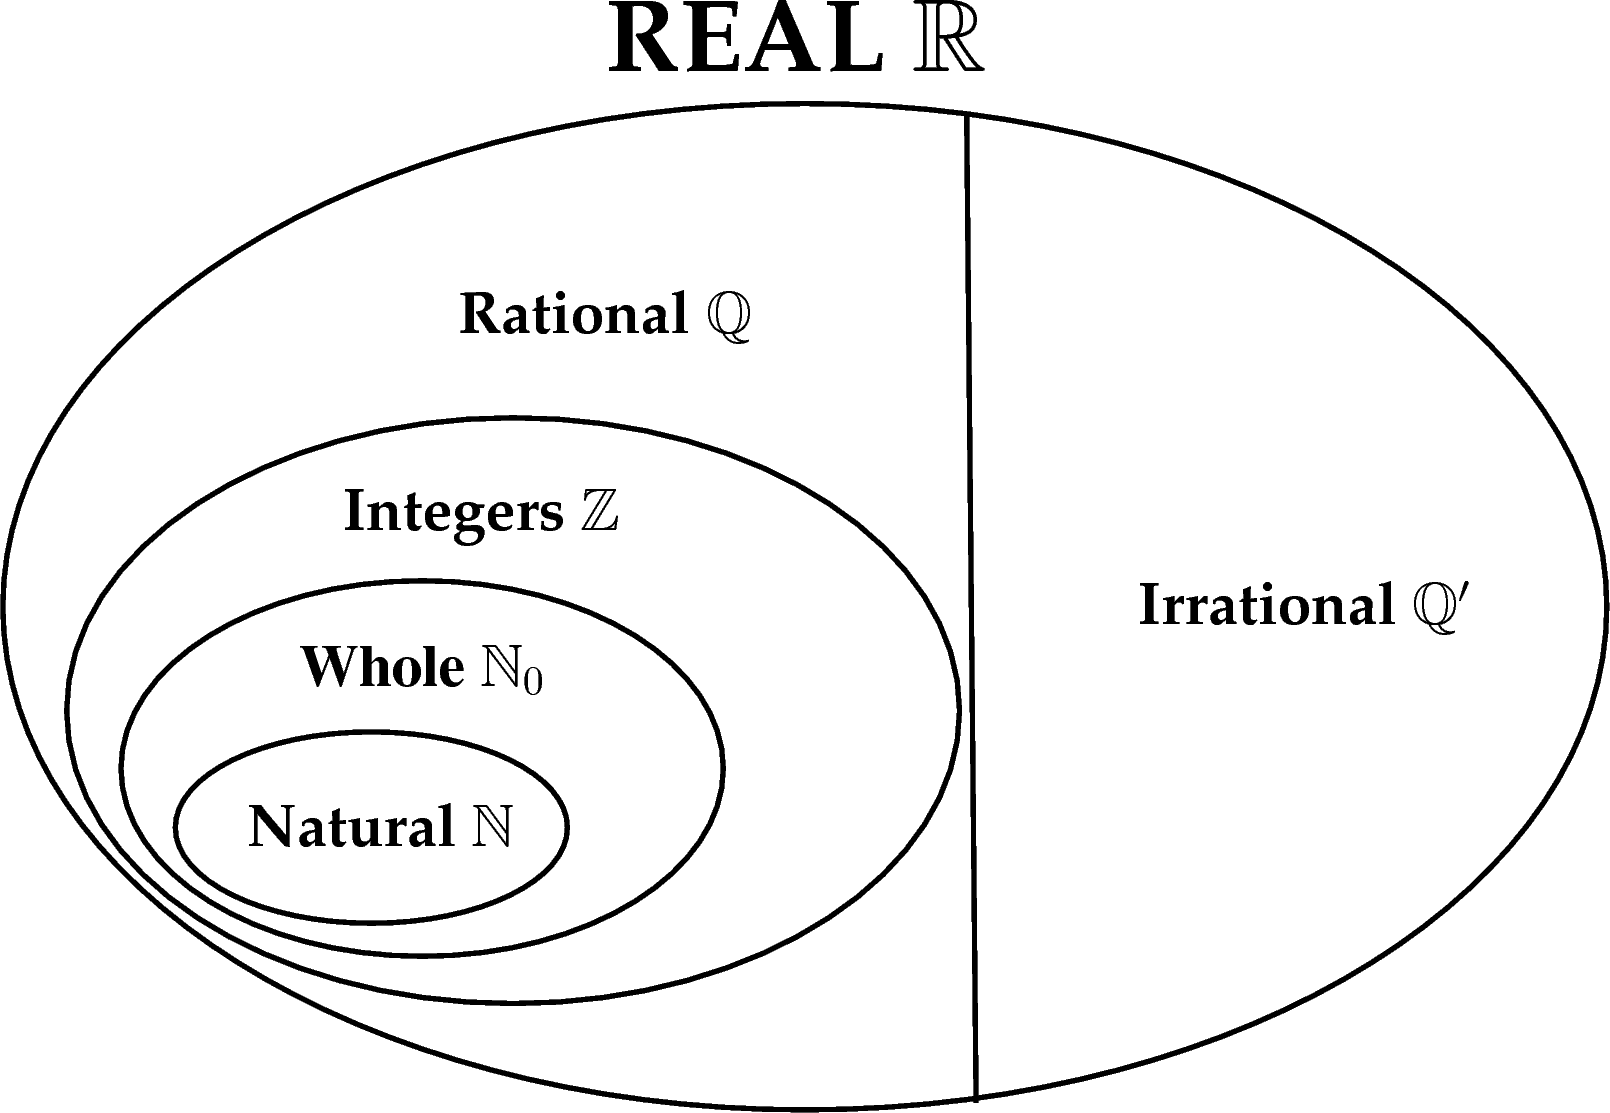
\includegraphics[width=9cm]{col11306.imgs/m38348_MG10C3_001.png} % m38348;MG10C3\_001.png;;;6.0;8.5;
\scalebox{1} % Change this value to rescale the drawing.
{
\begin{pspicture}(0,-4.764375)(14.481563,4.804375)
\psellipse[linewidth=0.04,dimen=outer](6.81,-0.484375)(6.81,4.28)
\psline[linewidth=0.04cm](8.18,3.695625)(8.26,-4.684375)
\psellipse[linewidth=0.04,dimen=outer](4.34,-1.364375)(3.8,2.5)
\psellipse[linewidth=0.04,dimen=outer](3.57,-1.854375)(2.57,1.61)
\usefont{T1}{ppl}{b}{n}
\rput(6.735781,4.350625){\Huge REAL $\mathbb{R}$}
\usefont{T1}{ppl}{b}{n}
\rput(11.03875,-0.484375){\Large Irrational $\mathbb{Q'}$}
\usefont{T1}{ppl}{b}{n}
\rput(5.11875,1.975625){\Large Rational $\mathbb{Q}$}
\usefont{T1}{ppl}{b}{n}
\rput(4.06875,0.275625){\Large Integers $\mathbb{Z}$}
\usefont{T1}{ppl}{b}{n}
\rput(3.21875,-2.324375){\Large Natural $\mathbb{N}$}
\psellipse[linewidth=0.04,dimen=outer](3.14,-2.354375)(1.68,0.83)
\usefont{T1}{ptm}{b}{n}
\rput(3.5735939,-1.024375){\Large Whole $\mathbb{N}_0$}
\end{pspicture} 
}
      \vspace{2pt}
    \vspace{.1in}
    \end{center}
 \end{figure}       
      \par 
      \label{m38348*id62554}The term whole number does not have a consistent definition. Various authors use
it in many different ways. We use the following definitions:\par 
      \label{m38348*id62559}\begin{itemize}[noitemsep]
            \label{m38348*uid1}\item natural numbers are (1, 2, 3, ...)
\label{m38348*uid2}\item whole numbers are (0, 1, 2, 3, ...)
\label{m38348*uid3}\item integers are (... -3, -2, -1, 0, 1, 2, 3, ....)
\end{itemize}
    \subsection{ Definition}
            \nopagebreak
            \label{m38348*cid4} $ \hspace{-5pt}\begin{array}{cccccccccccc}   \end{array} $ \hspace{2 pt}\raisebox{-5 pt}{
\includegraphics[width=0.5cm]{col11306.imgs/summary_www.png}} {(subsection shortcode: MG10036 )} \par 
      \label{m38348*id62607}The following numbers are all rational numbers.\par 
      \label{m38348*uid4}\nopagebreak\noindent{}
        
    \begin{equation}
    \frac{10}{1},\frac{21}{7},\frac{-1}{-3},\frac{10}{20},\frac{-3}{6}\tag{4.1}
      \end{equation}
      \label{m38348*id62687}You can see that all denominators and all numerators are integers.\par 
\label{m38348*fhsst!!!underscore!!!id138}\begin{definition}
	  \begin{tabular*}{15 cm}{m{15 mm}m{}}
	\hspace*{-50pt}  
\includegraphics[width=0.5in]{col11306.imgs/psflag2.png}   & \Definition{   \label{id2489628}\textbf{ Rational Number }} { \label{m38348*meaningfhsst!!!underscore!!!id138}
      \label{m38348*id62709}A rational number is any number which can be written as:\par 
      \label{m38348*uid6}\nopagebreak\noindent{}
        
    \begin{equation}
    \frac{a}{b}\tag{4.2}
      \end{equation}
      \label{m38348*id62732}where $a$ and $b$ are integers and $b\ne 0$. \par 
       } 
      \end{tabular*}
      \end{definition}
\label{m38348*eip-761}Note that because we can write $\frac{a}{-b}$
as $\frac{-a}{b}$
(in other words, one can always find an equivalent rational expression where $b\greatthan{}0$) mathematicians typically define rational numbers not as both $a$ and $b$ being integers, but rather that $a$ is an integer and $b$ is a natural number. This avoids having to worry about zero in the denominator. \par \label{m38348*notfhsst!!!underscore!!!id150}
\begin{tabular}{cc}
	   \hspace*{-50pt}\raisebox{-8 mm}{ 
\includegraphics[width=0.5in]{col11306.imgs/pstip2.png}  }& 
	\begin{minipage}{0.85\textwidth}
	\begin{note}
      {tip: }Only fractions which have a numerator and a denominator (that is not 0) that are integers
are rational numbers.
	\end{note}
	\end{minipage}
	\end{tabular}
	\par
      \label{m38348*id62778}This means that all integers are rational numbers, because they can be written with a denominator of 1.\par 
      \label{m38348*id62782}Therefore\par 
      \label{m38348*uid7}\nopagebreak\noindent{}
        
    \begin{equation}
    \frac{\sqrt{2}}{7},\frac{\pi }{20}\tag{4.3}
      \end{equation}
      \label{m38348*id62817}are \textbf{not examples} of rational numbers, because in each case, either the numerator or the denominator is not an integer.\par 
      \label{m38348*id62829}A number may not be written as an integer divided by another integer, but may still
be a rational number. This is because the results may be expressed
as an integer divided by an integer. The rule is, if a number can be written
as a fraction of integers, it is rational even if it can also be written in another
way as well. Here are two examples that might not look like rational numbers
at first glance but are because there are equivalent forms that are expressed as an
integer divided by another integer:\par 
      \label{m38348*uid8}\nopagebreak\noindent{}
    \begin{equation}    
    \frac{-1,33}{-3}=\frac{133}{300},\frac{-3}{6,39}=\frac{-300}{639}=\frac{-100}{213}\tag{4.4}
      \end{equation}
\label{m38348*secfhsst!!!underscore!!!id232}
            \subsubsection{Exercise: Rational Numbers }
            \nopagebreak
            \label{m38348*id63121}\begin{enumerate}[noitemsep, label=\textbf{\arabic*}. ] 
            \label{m38348*uid9}\item If $a$ is an integer, $b$ is an integer and $c$ is irrational, which of the following are rational numbers? 
\label{m38348*id734}\begin{enumerate}[noitemsep, label=\textbf{\alph*}. ] 
            \item $\frac{5}{6}$\newline
    \item $\frac{a}{3}$\newline
    \item $\frac{b}{2}$\newline
    \item $\frac{1}{c}$\end{enumerate}
        \label{m38348*uid10}\item If $\frac{a}{1}$ is a rational number, which of the following are valid values for $a$?\label{m38348*id7432}\begin{enumerate}[noitemsep, label=\textbf{\alph*}. ] 
            \item 1\item $-10$\item $\sqrt{2}$\item $2,1$\end{enumerate}
        \end{enumerate}
\par \raisebox{-5 pt}{
\includegraphics[width=0.5cm]{col11306.imgs/summary_www.png}} Find the answers with the shortcodes:
 \par \begin{tabular}[h]{cccccc}
 (1.) l35  &  (2.) l3N  & \end{tabular}
    \subsection{Decimal Numbers}
            \nopagebreak
            \label{m38348*cid5} $ \hspace{-5pt}\begin{array}{cccccccccccc}   \end{array} $ \hspace{2 pt}\raisebox{-5 pt}{
\includegraphics[width=0.5cm]{col11306.imgs/summary_www.png}} {(subsection shortcode: MG10037 )} \par 
      \label{m38348*id63345}All integers and fractions with integer numerators and denominators are rational numbers. There are two more forms of rational numbers.\par 
\label{m38348*secfhsst!!!underscore!!!id245}
            \subsubsection{  Investigation : Decimal Numbers }
            \nopagebreak
      \label{m38348*id63357}You can write the rational number
$\frac{1}{2}$ as the decimal number 0,5. Write the following numbers as
decimals:\par 
      \label{m38348*id63375}\begin{enumerate}[noitemsep, label=\textbf{\arabic*}. ] 
            \label{m38348*uid11}\item 
          $\frac{1}{4}$
        \label{m38348*uid12}\item 
          $\frac{1}{10}$
        \label{m38348*uid13}\item 
          $\frac{2}{5}$
        \label{m38348*uid14}\item 
          $\frac{1}{100}$
        \label{m38348*uid15}\item 
          $\frac{2}{3}$
        \end{enumerate}
      \label{m38348*id63486}Do the numbers after the decimal comma end or do they continue? If they continue, is there a repeating pattern to the numbers? \par 
      \label{m38348*id63495}You can write a rational number as a decimal number. Two types of decimal numbers can be written as rational numbers:\par 
      \label{m38348*id63500}\begin{enumerate}[noitemsep, label=\textbf{\arabic*}. ] 
            \label{m38348*uid16}\item decimal numbers that end or \textsl{terminate}, for example the fraction $\frac{4}{10}$ can be written as 0,4.
\label{m38348*uid17}\item decimal numbers that have a repeating pattern of numbers, for example the fraction $\frac{1}{3}$ can be written as 
$0,\dot{3}$. 
The dot represents recurring $3$'s i.e.,
$0,333...=0,\dot{3}$.
\end{enumerate}
      \label{m38348*id63576}For example, the rational number $\frac{5}{6}$ can be written in decimal notation as $0,8\dot{3}$ and similarly, the decimal number 0,25 can be written as a rational number as $\frac{1}{4}$.\par 
\label{m38348*notfhsst!!!underscore!!!id301}
\begin{tabular}{cc}
	   \hspace*{-50pt}\raisebox{-8 mm}{ 
\includegraphics[width=0.5in]{col11306.imgs/pstip2.png}  }& 
	\begin{minipage}{0.85\textwidth}
	\begin{note}
      {tip: }You can use a bar over the repeated numbers to indicate that the decimal is a repeating decimal.
	\end{note}
	\end{minipage}
	\end{tabular}
	\par
    \subsection{ Converting Terminating Decimals into Rational Numbers}
            \nopagebreak
            \label{m38348*cid6} $ \hspace{-5pt}\begin{array}{cccccccccccc}   \end{array} $ \hspace{2 pt}\raisebox{-5 pt}{
\includegraphics[width=0.5cm]{col11306.imgs/summary_www.png}} {(subsection shortcode: MG10038 )} \par 
      \label{m38348*id63646}A decimal number has an integer part and a fractional part. For example $10,589$ has an integer part of 10 and a fractional part of $0,589$ because $10+0,589=10,589$. The fractional part can be written as a rational number, i.e. with a numerator and a denominator that are integers.\par 
      \label{m38348*id63704}Each digit after the decimal point is a fraction with a denominator in increasing powers of ten. For example:\par 
      \label{m38348*id63708}\begin{itemize}[noitemsep]
            \label{m38348*uid18}\item $\frac{1}{10}$ is $0,1$\label{m38348*uid19}\item $\frac{1}{100}$ is $0,01$\end{itemize}
      \label{m38348*id63781}This means that:\par 
      \label{m38348*id63784}\nopagebreak\noindent{}
    \begin{equation}
    \begin{array}{ccc}\hfill 10,589& =& 10+\frac{5}{10}+\frac{8}{100}+\frac{9}{1000}\hfill \\ & =& 10\frac{589}{1000}\hfill \\ & =& \frac{10589}{1000}\hfill \end{array}\tag{4.5}
      \end{equation}
\label{m38348*secfhsst!!!underscore!!!id378}
            \subsubsection{ Exercise: Fractions }
            \nopagebreak
      \label{m38348*id63882}\begin{enumerate}[noitemsep, label=\textbf{\arabic*}. ] 
            \label{m38348*uid20}\item Write the following as fractions:\label{m38348*id7322}\begin{enumerate}[noitemsep, label=\textbf{\alph*}. ] 
            \item $0,1$\item $0,12$\item $0,58$\item $0,2589$\end{enumerate}
        \end{enumerate}
\par \raisebox{-5 pt}{
\includegraphics[width=0.5cm]{col11306.imgs/summary_www.png}} Find the answers with the shortcodes:
 \par \begin{tabular}[h]{cccccc}
 (1.) l3R  & \end{tabular}
    \subsection{ Converting Repeating Decimals into Rational Numbers}
            \nopagebreak
            \label{m38348*cid7} $ \hspace{-5pt}\begin{array}{cccccccccccc}   \end{array} $ \hspace{2 pt}\raisebox{-5 pt}{
\includegraphics[width=0.5cm]{col11306.imgs/summary_www.png}} {(subsection shortcode: MG10039 )} \par 
      \label{m38348*id63993}When the decimal is a repeating decimal, a bit more work is needed to write the fractional part of the decimal number as a fraction. We will explain by means of an example.\par 
      \label{m38348*id63998}If we wish to write $0,\dot{3}$ in the form $\frac{a}{b}$ (where $a$ and $b$ are integers) then we would proceed as follows
\par 
      \label{m38348*uid21}\nopagebreak\noindent{}
    \begin{equation}
    \begin{array}{cccc}\hfill x& =& 0,33333...\hfill & \\ \hfill 10x& =& 3,33333...\hfill & \text{multiply}\phantom{\rule{4.pt}{0ex}}\text{by}\phantom{\rule{4.pt}{0ex}}\text{10}\phantom{\rule{4.pt}{0ex}}\text{on}\phantom{\rule{4.pt}{0ex}}\text{both}\phantom{\rule{4.pt}{0ex}}\text{sides}\hfill \\ \hfill 9x& =& 3\hfill & \text{(}\text{subtracting}\phantom{\rule{4.pt}{0ex}}\text{the}\phantom{\rule{4.pt}{0ex}}\text{second}\phantom{\rule{4.pt}{0ex}}\text{equation}\phantom{\rule{4.pt}{0ex}}\text{from}\phantom{\rule{4.pt}{0ex}}\text{the}\phantom{\rule{4.pt}{0ex}}\text{first}\phantom{\rule{4.pt}{0ex}}\text{equation}\text{)}\hfill \\ \hfill x& =& \frac{3}{9}=\frac{1}{3}\hfill & \end{array}\tag{4.6}
      \end{equation}
      \label{m38348*id64237}And another example would be to write 
$5,\dot{4}\dot{3}\dot{2}$ 
as a rational fraction.
\par 
      \label{m38348*uid22}\nopagebreak\noindent{}
    \begin{equation}
    \begin{array}{cccc}\hfill x& =& 5,432432432...\hfill & \\ \hfill 1000x& =& 5432,432432432...\hfill & \text{multiply by\hspace{0.17em}}\phantom{\rule{4.pt}{0ex}}\text{1000}\phantom{\rule{4.pt}{0ex}}\text{on both sides}\\ \hfill \\ \hfill 999x& =& 5427\hfill & \text{(}\text{subtracting the second equation from the first equation}\text{)}\\ \hfill x& =& \frac{5427}{999}=\frac{201}{37}\hfill & \end{array}\tag{4.7}
      \end{equation}
      \label{m38348*id64459}For the first example, the decimal was multiplied by 10 and for the second example, the decimal was multiplied by 1000. This is because for the first example there was only one digit (i.e. 3) recurring, while for the second example there were three digits (i.e. 432) recurring.\par 
      \label{m38348*id64465}In general, if you have one digit recurring, then multiply by 10. If you have two digits recurring, then multiply by 100. If you have three digits recurring, then multiply by 1000. Can you spot the pattern yet?\par 
      \label{m38348*id64470}The number of zeros is the same as the number of recurring digits.\par 
      \label{m38348*id64474}Not all decimal numbers can be written as rational numbers. Why? Irrational decimal numbers like 
$\sqrt{2}=1,4142135...$
cannot be written with an integer numerator and denominator, because they do not have a pattern of recurring digits. However, when possible, you should try to use rational numbers or fractions instead of decimals.\par 
\label{m38348*secfhsst!!!underscore!!!id606}
            \subsubsection{Exercise: Repeated Decimal Notation }
            \nopagebreak
      \label{m38348*id64513}\begin{enumerate}[noitemsep, label=\textbf{\arabic*}. ] 
            \label{m38348*uid23}\item Write the following using the repeated decimal notation:
\label{m38348*id64529}\begin{enumerate}[noitemsep, label=\textbf{\alph*}. ] 
            \label{m38348*uid24}\item $0,11111111...$\label{m38348*uid25}\item $0,1212121212...$\label{m38348*uid26}\item $0,123123123123...$\label{m38348*uid27}\item $0,11414541454145...$\end{enumerate}
        \label{m38348*uid28}\item Write the following in decimal form, using the repeated decimal notation:
\label{m38348*id64650}\begin{enumerate}[noitemsep, label=\textbf{\alph*}. ] 
            \label{m38348*uid29}\item $\frac{2}{3}$\label{m38348*uid30}\item $1\frac{3}{11}$\label{m38348*uid31}\item $4\frac{5}{6}$\label{m38348*uid32}\item $2\frac{1}{9}$\end{enumerate}
        \label{m38348*uid33}\item Write the following decimals in fractional form:
\label{m38348*id64767}\begin{enumerate}[noitemsep, label=\textbf{\alph*}. ] 
            \label{m38348*uid34}\item $0,633\dot{3}$\label{m38348*uid35}\item $5,3131\overline{31}$\label{m38348*uid36}\item $0,99999\dot{9}$\end{enumerate}
        \end{enumerate}
\par \raisebox{-5 pt}{
\includegraphics[width=0.5cm]{col11306.imgs/summary_www.png}} Find the answers with the shortcodes:
 \par \begin{tabular}[h]{cccccc}
 (1.) l3U  &  (2.) l3n  &  (3.) l3Q  & \end{tabular}
         \section{Irrational Numbers}
    \setcounter{figure}{1}
    \setcounter{subfigure}{1}
    \label{m38349}
    \subsection{ Introduction}
            \nopagebreak
            \label{m38349*cid2} $ \hspace{-5pt}\begin{array}{cccccccccccc}   \end{array} $ \hspace{2 pt}\raisebox{-5 pt}{
\includegraphics[width=0.5cm]{col11306.imgs/summary_www.png}} {(subsection shortcode: MG10055 )} \par 
      \label{m38349*id324260}You have seen that repeating decimals may take a lot of paper and ink to write out. Not only is that impossible, but writing numbers out to many decimal places or \textsl{a high accuracy} is very inconvenient and rarely gives practical answers. For this reason we often estimate the number to a certain number of decimal places or to a given number of \textsl{significant figures}, which is even better.\par 
    \subsection{ Definition}
            \nopagebreak
            \label{m38349*cid3} $ \hspace{-5pt}\begin{array}{cccccccccccc}   \end{array} $ \hspace{2 pt}\raisebox{-5 pt}{
\includegraphics[width=0.5cm]{col11306.imgs/summary_www.png}} {(subsection shortcode: MG10056 )} \par \label{m38349*id324624}Irrational numbers are numbers that cannot be written as a fraction with the numerator and denominator as integers. This means that any number that is \textsl{not} a terminating decimal number or a repeating decimal number is irrational. Examples of irrational numbers are:\par 
      \label{m38349*id324635}\nopagebreak\noindent{}
        
    \begin{equation}
    \begin{array}{cc}\hfill \sqrt{2},\sqrt{3},\sqrt[3]{4},\pi ,\\ \hfill \frac{1+\sqrt{5}}{2}\approx 1,618\phantom{\rule{0.166667em}{0ex}}033\phantom{\rule{0.166667em}{0ex}}989\phantom{\rule{0.166667em}{0ex}}\end{array}\tag{7.1}
      \end{equation}
\label{m38349*notfhsst!!!underscore!!!id128}
\begin{tabular}{cc}
	   \hspace*{-50pt}\raisebox{-8 mm}{ 
\includegraphics[width=0.5in]{col11306.imgs/pstip2.png}  }& 
	\begin{minipage}{0.85\textwidth}
	\begin{note}
      {tip: }When irrational numbers are written in decimal form, they go on forever and
there is no repeated pattern of digits.
	\end{note}
	\end{minipage}
	\end{tabular}
	\par
      \label{m38349*id324739}If you are asked to identify whether a number is rational or irrational, first write the number in decimal form. If the number is terminated then it is rational. If it goes on forever, then look for a repeated pattern of digits. If there is no repeated pattern, then the number is irrational.\par 
      \label{m38349*id324745}When you write irrational numbers in decimal form, you may (if you have a lot of time and paper!) continue writing them for many, many decimal places. However, this is not convenient and it is often necessary to round off.\par 
\label{m38349*secfhsst!!!underscore!!!id133}
            \subsubsection{  Investigation : Irrational Numbers }
            \nopagebreak
      \label{m38349*id324757}Which of the following cannot be
written as a rational number?\par 
      \label{m38349*id324763}\textbf{Remember}: A rational number is a fraction with numerator and denominator as integers. Terminating decimal numbers or repeating decimal numbers are rational.\par 
      \label{m38349*id324775}\begin{enumerate}[noitemsep, label=\textbf{\arabic*}. ] 
            \label{m38349*uid1}\item 
          $\pi =3,14159265358979323846264338327950288419716939937510...$
        \label{m38349*uid2}\item $1,4$
\label{m38349*uid3}\item 
          $1,618\phantom{\rule{0.166667em}{0ex}}033\phantom{\rule{0.166667em}{0ex}}989\phantom{\rule{0.166667em}{0ex}}...$
        \label{m38349*uid4}\item $100$
\end{enumerate}
    \section{ Rounding Off}
            \nopagebreak
            \label{m38349*cid4} $ \hspace{-5pt}\begin{array}{cccccccccccc}   
\includegraphics[width=0.75cm]{col11306.imgs/summary_fullmarks.png} &   \end{array} $ \hspace{2 pt}\raisebox{-5 pt}{} {(section shortcode: MG10057 )} \par 
      \label{m38349*id324198}Rounding off or approximating a decimal number to a given number of decimal places is the quickest way to approximate a number. For example, if you wanted to round-off $2,6525272$ to three decimal places then you would first count three places after the decimal and place a $|$ between the third and fourth number after the decimal.\par 
      \label{m38349*id325085}\nopagebreak\noindent{}
        
    \begin{equation}
    2,652|5272\tag{7.2}
      \end{equation}
      \label{m38349*id325105}All numbers to the right of the $|$ are ignored after you determine whether the number in the third decimal place must be rounded up or rounded down. You \textsl{round up} the final digit if the first digit after the $|$ was greater than or equal to 5 and \textsl{round down} (leave the digit alone) otherwise. In the case that the first digit before the $|$ is 9 \textsl{and} you need to round up, then the 9 becomes a 0 and the second digit before the $|$ is rounded up.\par 
      \label{m38349*id325160}So, since the first digit after the $|$ is a 5, we must round up the digit in the third decimal place to a 3 and the final answer of $2,6525272$ rounded to three decimal places is\par 
      \label{m38349*id325186}\nopagebreak\noindent{}
        
    \begin{equation}
    2,653\tag{7.3}
      \end{equation}
\par
            \label{m38349*secfhsst!!!underscore!!!id199}\vspace{.5cm} 
      \noindent
      \hspace*{-30pt}
\includegraphics[width=0.5in]{col11306.imgs/pspencil2.png}   \raisebox{25mm}{   
      \begin{mdframed}[linewidth=4, leftmargin=40, rightmargin=40]  
      \begin{exercise}
    \noindent\textbf{Exercise 7.1:  Rounding-Off }
      \label{m38349*probfhsst!!!underscore!!!id200}
      \label{m38349*id325213}Round-off the following numbers to the indicated number of decimal places:\par 
      \label{m38349*id325219}\begin{enumerate}[noitemsep, label=\textbf{\arabic*}. ] 
            \leftskip=20pt\rightskip=\leftskip\label{m38349*uid5}\item $\frac{120}{99}=1,212121212\dot{1}\dot{2}$ to 3 decimal places
\label{m38349*uid6}\item $\pi =3,141592654...$ to 4 decimal places
\label{m38349*uid7}\item $\sqrt{3}=1,7320508...$ to 4 decimal places
\label{m38349*uid789}\item $2,78974526...$ to 3 decimal places\end{enumerate}
      \vspace{5pt}
      \label{m38349*solfhsst!!!underscore!!!id212}\noindent\textbf{Solution to Exercise } \label{m38349*listfhsst!!!underscore!!!id212}\begin{enumerate}[noitemsep, label=\textbf{Step} \textbf{\arabic*}. ] 
            \leftskip=20pt\rightskip=\leftskip\item  
      \label{m38349*id325360}\begin{enumerate}[noitemsep, label=\textbf{\alph*}. ] 
            \leftskip=20pt\rightskip=\leftskip\label{m38349*uid8}\item 
          $\frac{120}{99}=1,212|121212\dot{1}\dot{2}$
        \label{m38349*uid9}\item 
          $\pi =3,1415|92654...$
        \label{m38349*uid10}\item 
          $\sqrt{3}=1,7320|508...$
        \item $2,789|74526...$\end{enumerate}
      \item  
      \label{m38349*id325490}\begin{enumerate}[noitemsep, label=\textbf{\alph*}. ] 
            \leftskip=20pt\rightskip=\leftskip\label{m38349*uid11}\item The last digit of $\frac{120}{99}=1,212|121212\dot{1}\dot{2}$  must be rounded down.
\label{m38349*uid12}\item The last digit of $\pi =3,1415|92654...$ must be rounded up.
\label{m38349*uid13}\item The last digit of $\sqrt{3}=1,7320|508...$ must be rounded up.
\item  The last digit of $2,789|74526...$ must be rounded up. Since this is a 9, we replace it with a 0 and round up the second last digit.\end{enumerate}
      \item  
      \label{m38349*id325626}\begin{enumerate}[noitemsep, label=\textbf{\alph*}. ] 
            \leftskip=20pt\rightskip=\leftskip\label{m38349*uid14}\item $\frac{120}{99}=1,212$ rounded to 3 decimal places
\label{m38349*uid15}\item $\pi =3,1416$  rounded to 4 decimal places
\label{m38349*uid16}\item $\sqrt{3}=1,7321$ rounded to 4 decimal places
\item $2,790$\end{enumerate}
      \end{enumerate}
    \end{exercise}
    \end{mdframed}
    }
    \noindent
         \section{Estimating surds}
    \setcounter{figure}{1}
    \setcounter{subfigure}{1}
    \label{m38347}
%     \subsection{ Introduction}
            \nopagebreak
            \label{m38347*cid1} $ \hspace{-5pt}\begin{array}{cccccccccccc}   
\includegraphics[width=0.75cm]{col11306.imgs/summary_fullmarks.png} &   \end{array} $ \hspace{2 pt}\raisebox{-5 pt}{} {(subsection shortcode: MG10052 )} \par 
      \label{m38347*id258007}You should know by now what the ${n}^{\mathrm{th}}$ root of a number means. If the ${n}^{\mathrm{th}}$ root of a number cannot be simplified to a rational number, we call it a $\mathit{surd}$. For example, $\sqrt{2}$ and $\sqrt[3]{6}$ are surds, but $\sqrt{4}$ is not a surd because it can be simplified to the rational number 2.\par 
      \label{m38347*id258405}In this chapter we will only look at surds that look like $\sqrt[n]{a}$, where $a$ is any positive number, for example $\sqrt{7}$ or $\sqrt[3]{5}$. It is very common for $n$ to be 2, so we usually do not write $\sqrt[2]{a}$. Instead we write the surd as just $\sqrt{a}$, which is much easier to read.\par 
      \label{m38347*id258479}It is sometimes useful to know the approximate value of a surd without having to use a calculator. For example, we want to be able to estimate where a surd like $\sqrt{3}$ is on the number line. So how do we know where surds lie on the number line? From a calculator we know that $\sqrt{3}$ is equal to $1,73205...$. It is easy to see that $\sqrt{3}$ is above 1 and below 2. But to see this for other surds like $\sqrt{18}$ without using a calculator, you must first understand the following fact:\par 
\label{m38347*notfhsst!!!underscore!!!id71}
\begin{tabular}{cc}
	\hspace*{-50pt}\raisebox{-8 mm}{\hspace{-0.2in}
\includegraphics[width=0.75in]{col11306.imgs/psfact2.png} } & 
	\begin{minipage}{0.85\textwidth}
	\begin{note}
      {note: } 
If $a$ and $b$ are positive whole numbers, and $a\lessthan{}b$, then $\sqrt[n]{a}\lessthan{}\sqrt[n]{b}$. (Challenge: Can you explain why?)
	\end{note}
	\end{minipage}
	\end{tabular}
	\par
      \label{m38347*id258599}If you don't believe this fact, check it for a few numbers to convince yourself it is true.\par 
      \label{m38347*id258603}How do we use this fact to help us guess what $\sqrt{18}$ is? Well, you can easily see that $18\lessthan{}25$. Using our rule, we also know that $\sqrt{18}\lessthan{}\sqrt{25}$. But we know that ${5}^{2}=25$ so that $\sqrt{25}=5$. Now it is easy to simplify to get $\sqrt{18}\lessthan{}5$. Now we have a better idea of what $\sqrt{18}$ is.\par 
      \label{m38347*id258700}Now we know that $\sqrt{18}$ is less than 5, but this is only half the story. We can use the same trick again, but this time with 18 on the right-hand side. You will agree that $16\lessthan{}18$. Using our rule again, we also know that $\sqrt{16}\lessthan{}\sqrt{18}$. But we know that 16 is a perfect square, so we can simplify $\sqrt{16}$ to 4, and so we get $4\lessthan{}\sqrt{18}$!\par 
      \label{m38347*id258766}As you can see, we have shown that $\sqrt{18}$ is between 4 and 5. If we check on our calculator, we can see that $\sqrt{18}=4,1231...$, and the idea was right! You will notice that our idea used perfect squares that were close to the number 18. We found the largest perfect square smaller than 18 was ${4}^{2}=16$, and the smallest perfect square greater than 18 was ${5}^{2}=25$. Here is a quick summary of what a perfect square or cube is:\par 
\label{m38347*notfhsst!!!underscore!!!id78}
\begin{tabular}{cc}
	\hspace*{-50pt}\raisebox{-8 mm}{\hspace{-0.2in}
\includegraphics[width=0.75in]{col11306.imgs/psfact2.png} } & 
	\begin{minipage}{0.85\textwidth}
	\begin{note}
      {note: } A perfect square is the number obtained when an integer is squared. For example, 9 is a perfect square since ${3}^{2}=9$. Similarly, a perfect cube is a number which is the cube of an integer. For example, 27 is a perfect cube, because ${3}^{3}=27$.
	\end{note}
	\end{minipage}
	\end{tabular}
	\par
      \label{m38347*id258890}To make it easier to use our idea, we will create a list of some of the perfect squares and perfect cubes. The list is shown in Table 6.1.\par 
    % \textbf{m38347*uid1}\par
    % how many colspecs?  3
          % name: cnx:colspec
            % colnum: 1
            % colwidth: 10*
            % latex-name: columna
            % colname: 
            % align/tgroup-align/default: //left
            % -------------------------
            % name: cnx:colspec
            % colnum: 2
            % colwidth: 10*
            % latex-name: columnb
            % colname: 
            % align/tgroup-align/default: //left
            % -------------------------
            % name: cnx:colspec
            % colnum: 3
            % colwidth: 10*
            % latex-name: columnc
            % colname: 
            % align/tgroup-align/default: //left
            % -------------------------
    \setlength\mytablespace{6\tabcolsep}
    \addtolength\mytablespace{4\arrayrulewidth}
    \setlength\mytablewidth{\linewidth}
    \setlength\mytableroom{\mytablewidth}
    \addtolength\mytableroom{-\mytablespace}
    \setlength\myfixedwidth{0pt}
    \setlength\mystarwidth{\mytableroom}
        \addtolength\mystarwidth{-\myfixedwidth}
        \divide\mystarwidth 30
      % ----- Begin capturing width of table in LR mode woof
      \settowidth{\mytableboxwidth}{\begin{tabular}[t]{|l|l|l|}\hline
    % count in rowspan-info-nodeset: 3
    % align/colidx: left,1
    % rowcount: '0' | start: 'false' | colidx: '1'
        % Formatting a regular cell and recurring on the next sibling
        Integer &
      % align/colidx: left,2
    % rowcount: '0' | start: 'false' | colidx: '2'
        % Formatting a regular cell and recurring on the next sibling
        Perfect Square &
      % align/colidx: left,3
    % rowcount: '0' | start: 'false' | colidx: '3'
        % Formatting a regular cell and recurring on the next sibling
        Perfect Cube% make-rowspan-placeholders
    % rowspan info: col1 '0' | 'false' | '' || col2 '0' | 'false' | '' || col3 '0' | 'false' | ''
     \tabularnewline\cline{1-1}\cline{2-2}\cline{3-3}
      %--------------------------------------------------------------------
    % align/colidx: left,1
    % rowcount: '0' | start: 'false' | colidx: '1'
        % Formatting a regular cell and recurring on the next sibling
        0 &
      % align/colidx: left,2
    % rowcount: '0' | start: 'false' | colidx: '2'
        % Formatting a regular cell and recurring on the next sibling
        0 &
      % align/colidx: left,3
    % rowcount: '0' | start: 'false' | colidx: '3'
        % Formatting a regular cell and recurring on the next sibling
        0% make-rowspan-placeholders
    % rowspan info: col1 '0' | 'false' | '' || col2 '0' | 'false' | '' || col3 '0' | 'false' | ''
     \tabularnewline\cline{1-1}\cline{2-2}\cline{3-3}
      %--------------------------------------------------------------------
    % align/colidx: left,1
    % rowcount: '0' | start: 'false' | colidx: '1'
        % Formatting a regular cell and recurring on the next sibling
        1 &
      % align/colidx: left,2
    % rowcount: '0' | start: 'false' | colidx: '2'
        % Formatting a regular cell and recurring on the next sibling
        1 &
      % align/colidx: left,3
    % rowcount: '0' | start: 'false' | colidx: '3'
        % Formatting a regular cell and recurring on the next sibling
        1% make-rowspan-placeholders
    % rowspan info: col1 '0' | 'false' | '' || col2 '0' | 'false' | '' || col3 '0' | 'false' | ''
     \tabularnewline\cline{1-1}\cline{2-2}\cline{3-3}
      %--------------------------------------------------------------------
    % align/colidx: left,1
    % rowcount: '0' | start: 'false' | colidx: '1'
        % Formatting a regular cell and recurring on the next sibling
        2 &
      % align/colidx: left,2
    % rowcount: '0' | start: 'false' | colidx: '2'
        % Formatting a regular cell and recurring on the next sibling
        4 &
      % align/colidx: left,3
    % rowcount: '0' | start: 'false' | colidx: '3'
        % Formatting a regular cell and recurring on the next sibling
        8% make-rowspan-placeholders
    % rowspan info: col1 '0' | 'false' | '' || col2 '0' | 'false' | '' || col3 '0' | 'false' | ''
     \tabularnewline\cline{1-1}\cline{2-2}\cline{3-3}
      %--------------------------------------------------------------------
    % align/colidx: left,1
    % rowcount: '0' | start: 'false' | colidx: '1'
        % Formatting a regular cell and recurring on the next sibling
        3 &
      % align/colidx: left,2
    % rowcount: '0' | start: 'false' | colidx: '2'
        % Formatting a regular cell and recurring on the next sibling
        9 &
      % align/colidx: left,3
    % rowcount: '0' | start: 'false' | colidx: '3'
        % Formatting a regular cell and recurring on the next sibling
        27% make-rowspan-placeholders
    % rowspan info: col1 '0' | 'false' | '' || col2 '0' | 'false' | '' || col3 '0' | 'false' | ''
     \tabularnewline\cline{1-1}\cline{2-2}\cline{3-3}
      %--------------------------------------------------------------------
    % align/colidx: left,1
    % rowcount: '0' | start: 'false' | colidx: '1'
        % Formatting a regular cell and recurring on the next sibling
        4 &
      % align/colidx: left,2
    % rowcount: '0' | start: 'false' | colidx: '2'
        % Formatting a regular cell and recurring on the next sibling
        16 &
      % align/colidx: left,3
    % rowcount: '0' | start: 'false' | colidx: '3'
        % Formatting a regular cell and recurring on the next sibling
        64% make-rowspan-placeholders
    % rowspan info: col1 '0' | 'false' | '' || col2 '0' | 'false' | '' || col3 '0' | 'false' | ''
     \tabularnewline\cline{1-1}\cline{2-2}\cline{3-3}
      %--------------------------------------------------------------------
    % align/colidx: left,1
    % rowcount: '0' | start: 'false' | colidx: '1'
        % Formatting a regular cell and recurring on the next sibling
        5 &
      % align/colidx: left,2
    % rowcount: '0' | start: 'false' | colidx: '2'
        % Formatting a regular cell and recurring on the next sibling
        25 &
      % align/colidx: left,3
    % rowcount: '0' | start: 'false' | colidx: '3'
        % Formatting a regular cell and recurring on the next sibling
        125% make-rowspan-placeholders
    % rowspan info: col1 '0' | 'false' | '' || col2 '0' | 'false' | '' || col3 '0' | 'false' | ''
     \tabularnewline\cline{1-1}\cline{2-2}\cline{3-3}
      %--------------------------------------------------------------------
    % align/colidx: left,1
    % rowcount: '0' | start: 'false' | colidx: '1'
        % Formatting a regular cell and recurring on the next sibling
        6 &
      % align/colidx: left,2
    % rowcount: '0' | start: 'false' | colidx: '2'
        % Formatting a regular cell and recurring on the next sibling
        36 &
      % align/colidx: left,3
    % rowcount: '0' | start: 'false' | colidx: '3'
        % Formatting a regular cell and recurring on the next sibling
        216% make-rowspan-placeholders
    % rowspan info: col1 '0' | 'false' | '' || col2 '0' | 'false' | '' || col3 '0' | 'false' | ''
     \tabularnewline\cline{1-1}\cline{2-2}\cline{3-3}
      %--------------------------------------------------------------------
    % align/colidx: left,1
    % rowcount: '0' | start: 'false' | colidx: '1'
        % Formatting a regular cell and recurring on the next sibling
        7 &
      % align/colidx: left,2
    % rowcount: '0' | start: 'false' | colidx: '2'
        % Formatting a regular cell and recurring on the next sibling
        49 &
      % align/colidx: left,3
    % rowcount: '0' | start: 'false' | colidx: '3'
        % Formatting a regular cell and recurring on the next sibling
        343% make-rowspan-placeholders
    % rowspan info: col1 '0' | 'false' | '' || col2 '0' | 'false' | '' || col3 '0' | 'false' | ''
     \tabularnewline\cline{1-1}\cline{2-2}\cline{3-3}
      %--------------------------------------------------------------------
    % align/colidx: left,1
    % rowcount: '0' | start: 'false' | colidx: '1'
        % Formatting a regular cell and recurring on the next sibling
        8 &
      % align/colidx: left,2
    % rowcount: '0' | start: 'false' | colidx: '2'
        % Formatting a regular cell and recurring on the next sibling
        64 &
      % align/colidx: left,3
    % rowcount: '0' | start: 'false' | colidx: '3'
        % Formatting a regular cell and recurring on the next sibling
        512% make-rowspan-placeholders
    % rowspan info: col1 '0' | 'false' | '' || col2 '0' | 'false' | '' || col3 '0' | 'false' | ''
     \tabularnewline\cline{1-1}\cline{2-2}\cline{3-3}
      %--------------------------------------------------------------------
    % align/colidx: left,1
    % rowcount: '0' | start: 'false' | colidx: '1'
        % Formatting a regular cell and recurring on the next sibling
        9 &
      % align/colidx: left,2
    % rowcount: '0' | start: 'false' | colidx: '2'
        % Formatting a regular cell and recurring on the next sibling
        81 &
      % align/colidx: left,3
    % rowcount: '0' | start: 'false' | colidx: '3'
        % Formatting a regular cell and recurring on the next sibling
        729% make-rowspan-placeholders
    % rowspan info: col1 '0' | 'false' | '' || col2 '0' | 'false' | '' || col3 '0' | 'false' | ''
     \tabularnewline\cline{1-1}\cline{2-2}\cline{3-3}
      %--------------------------------------------------------------------
    % align/colidx: left,1
    % rowcount: '0' | start: 'false' | colidx: '1'
        % Formatting a regular cell and recurring on the next sibling
        10 &
      % align/colidx: left,2
    % rowcount: '0' | start: 'false' | colidx: '2'
        % Formatting a regular cell and recurring on the next sibling
        100 &
      % align/colidx: left,3
    % rowcount: '0' | start: 'false' | colidx: '3'
        % Formatting a regular cell and recurring on the next sibling
        1000% make-rowspan-placeholders
    % rowspan info: col1 '0' | 'false' | '' || col2 '0' | 'false' | '' || col3 '0' | 'false' | ''
     \tabularnewline\cline{1-1}\cline{2-2}\cline{3-3}
      %--------------------------------------------------------------------
    \end{tabular}} % end mytableboxwidth set      
      % ----- End capturing width of table in LR mode
        % ----- LR or paragraph mode: must test
        % ----- Begin capturing height of table
        \settoheight{\mytableboxheight}{\begin{tabular}[t]{|l|l|l|}\hline
    % count in rowspan-info-nodeset: 3
    % align/colidx: left,1
    % rowcount: '0' | start: 'false' | colidx: '1'
        % Formatting a regular cell and recurring on the next sibling
        Integer &
      % align/colidx: left,2
    % rowcount: '0' | start: 'false' | colidx: '2'
        % Formatting a regular cell and recurring on the next sibling
        Perfect Square &
      % align/colidx: left,3
    % rowcount: '0' | start: 'false' | colidx: '3'
        % Formatting a regular cell and recurring on the next sibling
        Perfect Cube% make-rowspan-placeholders
    % rowspan info: col1 '0' | 'false' | '' || col2 '0' | 'false' | '' || col3 '0' | 'false' | ''
     \tabularnewline\cline{1-1}\cline{2-2}\cline{3-3}
      %--------------------------------------------------------------------
    % align/colidx: left,1
    % rowcount: '0' | start: 'false' | colidx: '1'
        % Formatting a regular cell and recurring on the next sibling
        0 &
      % align/colidx: left,2
    % rowcount: '0' | start: 'false' | colidx: '2'
        % Formatting a regular cell and recurring on the next sibling
        0 &
      % align/colidx: left,3
    % rowcount: '0' | start: 'false' | colidx: '3'
        % Formatting a regular cell and recurring on the next sibling
        0% make-rowspan-placeholders
    % rowspan info: col1 '0' | 'false' | '' || col2 '0' | 'false' | '' || col3 '0' | 'false' | ''
     \tabularnewline\cline{1-1}\cline{2-2}\cline{3-3}
      %--------------------------------------------------------------------
    % align/colidx: left,1
    % rowcount: '0' | start: 'false' | colidx: '1'
        % Formatting a regular cell and recurring on the next sibling
        1 &
      % align/colidx: left,2
    % rowcount: '0' | start: 'false' | colidx: '2'
        % Formatting a regular cell and recurring on the next sibling
        1 &
      % align/colidx: left,3
    % rowcount: '0' | start: 'false' | colidx: '3'
        % Formatting a regular cell and recurring on the next sibling
        1% make-rowspan-placeholders
    % rowspan info: col1 '0' | 'false' | '' || col2 '0' | 'false' | '' || col3 '0' | 'false' | ''
     \tabularnewline\cline{1-1}\cline{2-2}\cline{3-3}
      %--------------------------------------------------------------------
    % align/colidx: left,1
    % rowcount: '0' | start: 'false' | colidx: '1'
        % Formatting a regular cell and recurring on the next sibling
        2 &
      % align/colidx: left,2
    % rowcount: '0' | start: 'false' | colidx: '2'
        % Formatting a regular cell and recurring on the next sibling
        4 &
      % align/colidx: left,3
    % rowcount: '0' | start: 'false' | colidx: '3'
        % Formatting a regular cell and recurring on the next sibling
        8% make-rowspan-placeholders
    % rowspan info: col1 '0' | 'false' | '' || col2 '0' | 'false' | '' || col3 '0' | 'false' | ''
     \tabularnewline\cline{1-1}\cline{2-2}\cline{3-3}
      %--------------------------------------------------------------------
    % align/colidx: left,1
    % rowcount: '0' | start: 'false' | colidx: '1'
        % Formatting a regular cell and recurring on the next sibling
        3 &
      % align/colidx: left,2
    % rowcount: '0' | start: 'false' | colidx: '2'
        % Formatting a regular cell and recurring on the next sibling
        9 &
      % align/colidx: left,3
    % rowcount: '0' | start: 'false' | colidx: '3'
        % Formatting a regular cell and recurring on the next sibling
        27% make-rowspan-placeholders
    % rowspan info: col1 '0' | 'false' | '' || col2 '0' | 'false' | '' || col3 '0' | 'false' | ''
     \tabularnewline\cline{1-1}\cline{2-2}\cline{3-3}
      %--------------------------------------------------------------------
    % align/colidx: left,1
    % rowcount: '0' | start: 'false' | colidx: '1'
        % Formatting a regular cell and recurring on the next sibling
        4 &
      % align/colidx: left,2
    % rowcount: '0' | start: 'false' | colidx: '2'
        % Formatting a regular cell and recurring on the next sibling
        16 &
      % align/colidx: left,3
    % rowcount: '0' | start: 'false' | colidx: '3'
        % Formatting a regular cell and recurring on the next sibling
        64% make-rowspan-placeholders
    % rowspan info: col1 '0' | 'false' | '' || col2 '0' | 'false' | '' || col3 '0' | 'false' | ''
     \tabularnewline\cline{1-1}\cline{2-2}\cline{3-3}
      %--------------------------------------------------------------------
    % align/colidx: left,1
    % rowcount: '0' | start: 'false' | colidx: '1'
        % Formatting a regular cell and recurring on the next sibling
        5 &
      % align/colidx: left,2
    % rowcount: '0' | start: 'false' | colidx: '2'
        % Formatting a regular cell and recurring on the next sibling
        25 &
      % align/colidx: left,3
    % rowcount: '0' | start: 'false' | colidx: '3'
        % Formatting a regular cell and recurring on the next sibling
        125% make-rowspan-placeholders
    % rowspan info: col1 '0' | 'false' | '' || col2 '0' | 'false' | '' || col3 '0' | 'false' | ''
     \tabularnewline\cline{1-1}\cline{2-2}\cline{3-3}
      %--------------------------------------------------------------------
    % align/colidx: left,1
    % rowcount: '0' | start: 'false' | colidx: '1'
        % Formatting a regular cell and recurring on the next sibling
        6 &
      % align/colidx: left,2
    % rowcount: '0' | start: 'false' | colidx: '2'
        % Formatting a regular cell and recurring on the next sibling
        36 &
      % align/colidx: left,3
    % rowcount: '0' | start: 'false' | colidx: '3'
        % Formatting a regular cell and recurring on the next sibling
        216% make-rowspan-placeholders
    % rowspan info: col1 '0' | 'false' | '' || col2 '0' | 'false' | '' || col3 '0' | 'false' | ''
     \tabularnewline\cline{1-1}\cline{2-2}\cline{3-3}
      %--------------------------------------------------------------------
    % align/colidx: left,1
    % rowcount: '0' | start: 'false' | colidx: '1'
        % Formatting a regular cell and recurring on the next sibling
        7 &
      % align/colidx: left,2
    % rowcount: '0' | start: 'false' | colidx: '2'
        % Formatting a regular cell and recurring on the next sibling
        49 &
      % align/colidx: left,3
    % rowcount: '0' | start: 'false' | colidx: '3'
        % Formatting a regular cell and recurring on the next sibling
        343% make-rowspan-placeholders
    % rowspan info: col1 '0' | 'false' | '' || col2 '0' | 'false' | '' || col3 '0' | 'false' | ''
     \tabularnewline\cline{1-1}\cline{2-2}\cline{3-3}
      %--------------------------------------------------------------------
    % align/colidx: left,1
    % rowcount: '0' | start: 'false' | colidx: '1'
        % Formatting a regular cell and recurring on the next sibling
        8 &
      % align/colidx: left,2
    % rowcount: '0' | start: 'false' | colidx: '2'
        % Formatting a regular cell and recurring on the next sibling
        64 &
      % align/colidx: left,3
    % rowcount: '0' | start: 'false' | colidx: '3'
        % Formatting a regular cell and recurring on the next sibling
        512% make-rowspan-placeholders
    % rowspan info: col1 '0' | 'false' | '' || col2 '0' | 'false' | '' || col3 '0' | 'false' | ''
     \tabularnewline\cline{1-1}\cline{2-2}\cline{3-3}
      %--------------------------------------------------------------------
    % align/colidx: left,1
    % rowcount: '0' | start: 'false' | colidx: '1'
        % Formatting a regular cell and recurring on the next sibling
        9 &
      % align/colidx: left,2
    % rowcount: '0' | start: 'false' | colidx: '2'
        % Formatting a regular cell and recurring on the next sibling
        81 &
      % align/colidx: left,3
    % rowcount: '0' | start: 'false' | colidx: '3'
        % Formatting a regular cell and recurring on the next sibling
        729% make-rowspan-placeholders
    % rowspan info: col1 '0' | 'false' | '' || col2 '0' | 'false' | '' || col3 '0' | 'false' | ''
     \tabularnewline\cline{1-1}\cline{2-2}\cline{3-3}
      %--------------------------------------------------------------------
    % align/colidx: left,1
    % rowcount: '0' | start: 'false' | colidx: '1'
        % Formatting a regular cell and recurring on the next sibling
        10 &
      % align/colidx: left,2
    % rowcount: '0' | start: 'false' | colidx: '2'
        % Formatting a regular cell and recurring on the next sibling
        100 &
      % align/colidx: left,3
    % rowcount: '0' | start: 'false' | colidx: '3'
        % Formatting a regular cell and recurring on the next sibling
        1000% make-rowspan-placeholders
    % rowspan info: col1 '0' | 'false' | '' || col2 '0' | 'false' | '' || col3 '0' | 'false' | ''
     \tabularnewline\cline{1-1}\cline{2-2}\cline{3-3}
      %--------------------------------------------------------------------
    \end{tabular}} % end mytableboxheight set
        \settodepth{\mytableboxdepth}{\begin{tabular}[t]{|l|l|l|}\hline
    % count in rowspan-info-nodeset: 3
    % align/colidx: left,1
    % rowcount: '0' | start: 'false' | colidx: '1'
        % Formatting a regular cell and recurring on the next sibling
        Integer &
      % align/colidx: left,2
    % rowcount: '0' | start: 'false' | colidx: '2'
        % Formatting a regular cell and recurring on the next sibling
        Perfect Square &
      % align/colidx: left,3
    % rowcount: '0' | start: 'false' | colidx: '3'
        % Formatting a regular cell and recurring on the next sibling
        Perfect Cube% make-rowspan-placeholders
    % rowspan info: col1 '0' | 'false' | '' || col2 '0' | 'false' | '' || col3 '0' | 'false' | ''
     \tabularnewline\cline{1-1}\cline{2-2}\cline{3-3}
      %--------------------------------------------------------------------
    % align/colidx: left,1
    % rowcount: '0' | start: 'false' | colidx: '1'
        % Formatting a regular cell and recurring on the next sibling
        0 &
      % align/colidx: left,2
    % rowcount: '0' | start: 'false' | colidx: '2'
        % Formatting a regular cell and recurring on the next sibling
        0 &
      % align/colidx: left,3
    % rowcount: '0' | start: 'false' | colidx: '3'
        % Formatting a regular cell and recurring on the next sibling
        0% make-rowspan-placeholders
    % rowspan info: col1 '0' | 'false' | '' || col2 '0' | 'false' | '' || col3 '0' | 'false' | ''
     \tabularnewline\cline{1-1}\cline{2-2}\cline{3-3}
      %--------------------------------------------------------------------
    % align/colidx: left,1
    % rowcount: '0' | start: 'false' | colidx: '1'
        % Formatting a regular cell and recurring on the next sibling
        1 &
      % align/colidx: left,2
    % rowcount: '0' | start: 'false' | colidx: '2'
        % Formatting a regular cell and recurring on the next sibling
        1 &
      % align/colidx: left,3
    % rowcount: '0' | start: 'false' | colidx: '3'
        % Formatting a regular cell and recurring on the next sibling
        1% make-rowspan-placeholders
    % rowspan info: col1 '0' | 'false' | '' || col2 '0' | 'false' | '' || col3 '0' | 'false' | ''
     \tabularnewline\cline{1-1}\cline{2-2}\cline{3-3}
      %--------------------------------------------------------------------
    % align/colidx: left,1
    % rowcount: '0' | start: 'false' | colidx: '1'
        % Formatting a regular cell and recurring on the next sibling
        2 &
      % align/colidx: left,2
    % rowcount: '0' | start: 'false' | colidx: '2'
        % Formatting a regular cell and recurring on the next sibling
        4 &
      % align/colidx: left,3
    % rowcount: '0' | start: 'false' | colidx: '3'
        % Formatting a regular cell and recurring on the next sibling
        8% make-rowspan-placeholders
    % rowspan info: col1 '0' | 'false' | '' || col2 '0' | 'false' | '' || col3 '0' | 'false' | ''
     \tabularnewline\cline{1-1}\cline{2-2}\cline{3-3}
      %--------------------------------------------------------------------
    % align/colidx: left,1
    % rowcount: '0' | start: 'false' | colidx: '1'
        % Formatting a regular cell and recurring on the next sibling
        3 &
      % align/colidx: left,2
    % rowcount: '0' | start: 'false' | colidx: '2'
        % Formatting a regular cell and recurring on the next sibling
        9 &
      % align/colidx: left,3
    % rowcount: '0' | start: 'false' | colidx: '3'
        % Formatting a regular cell and recurring on the next sibling
        27% make-rowspan-placeholders
    % rowspan info: col1 '0' | 'false' | '' || col2 '0' | 'false' | '' || col3 '0' | 'false' | ''
     \tabularnewline\cline{1-1}\cline{2-2}\cline{3-3}
      %--------------------------------------------------------------------
    % align/colidx: left,1
    % rowcount: '0' | start: 'false' | colidx: '1'
        % Formatting a regular cell and recurring on the next sibling
        4 &
      % align/colidx: left,2
    % rowcount: '0' | start: 'false' | colidx: '2'
        % Formatting a regular cell and recurring on the next sibling
        16 &
      % align/colidx: left,3
    % rowcount: '0' | start: 'false' | colidx: '3'
        % Formatting a regular cell and recurring on the next sibling
        64% make-rowspan-placeholders
    % rowspan info: col1 '0' | 'false' | '' || col2 '0' | 'false' | '' || col3 '0' | 'false' | ''
     \tabularnewline\cline{1-1}\cline{2-2}\cline{3-3}
      %--------------------------------------------------------------------
    % align/colidx: left,1
    % rowcount: '0' | start: 'false' | colidx: '1'
        % Formatting a regular cell and recurring on the next sibling
        5 &
      % align/colidx: left,2
    % rowcount: '0' | start: 'false' | colidx: '2'
        % Formatting a regular cell and recurring on the next sibling
        25 &
      % align/colidx: left,3
    % rowcount: '0' | start: 'false' | colidx: '3'
        % Formatting a regular cell and recurring on the next sibling
        125% make-rowspan-placeholders
    % rowspan info: col1 '0' | 'false' | '' || col2 '0' | 'false' | '' || col3 '0' | 'false' | ''
     \tabularnewline\cline{1-1}\cline{2-2}\cline{3-3}
      %--------------------------------------------------------------------
    % align/colidx: left,1
    % rowcount: '0' | start: 'false' | colidx: '1'
        % Formatting a regular cell and recurring on the next sibling
        6 &
      % align/colidx: left,2
    % rowcount: '0' | start: 'false' | colidx: '2'
        % Formatting a regular cell and recurring on the next sibling
        36 &
      % align/colidx: left,3
    % rowcount: '0' | start: 'false' | colidx: '3'
        % Formatting a regular cell and recurring on the next sibling
        216% make-rowspan-placeholders
    % rowspan info: col1 '0' | 'false' | '' || col2 '0' | 'false' | '' || col3 '0' | 'false' | ''
     \tabularnewline\cline{1-1}\cline{2-2}\cline{3-3}
      %--------------------------------------------------------------------
    % align/colidx: left,1
    % rowcount: '0' | start: 'false' | colidx: '1'
        % Formatting a regular cell and recurring on the next sibling
        7 &
      % align/colidx: left,2
    % rowcount: '0' | start: 'false' | colidx: '2'
        % Formatting a regular cell and recurring on the next sibling
        49 &
      % align/colidx: left,3
    % rowcount: '0' | start: 'false' | colidx: '3'
        % Formatting a regular cell and recurring on the next sibling
        343% make-rowspan-placeholders
    % rowspan info: col1 '0' | 'false' | '' || col2 '0' | 'false' | '' || col3 '0' | 'false' | ''
     \tabularnewline\cline{1-1}\cline{2-2}\cline{3-3}
      %--------------------------------------------------------------------
    % align/colidx: left,1
    % rowcount: '0' | start: 'false' | colidx: '1'
        % Formatting a regular cell and recurring on the next sibling
        8 &
      % align/colidx: left,2
    % rowcount: '0' | start: 'false' | colidx: '2'
        % Formatting a regular cell and recurring on the next sibling
        64 &
      % align/colidx: left,3
    % rowcount: '0' | start: 'false' | colidx: '3'
        % Formatting a regular cell and recurring on the next sibling
        512% make-rowspan-placeholders
    % rowspan info: col1 '0' | 'false' | '' || col2 '0' | 'false' | '' || col3 '0' | 'false' | ''
     \tabularnewline\cline{1-1}\cline{2-2}\cline{3-3}
      %--------------------------------------------------------------------
    % align/colidx: left,1
    % rowcount: '0' | start: 'false' | colidx: '1'
        % Formatting a regular cell and recurring on the next sibling
        9 &
      % align/colidx: left,2
    % rowcount: '0' | start: 'false' | colidx: '2'
        % Formatting a regular cell and recurring on the next sibling
        81 &
      % align/colidx: left,3
    % rowcount: '0' | start: 'false' | colidx: '3'
        % Formatting a regular cell and recurring on the next sibling
        729% make-rowspan-placeholders
    % rowspan info: col1 '0' | 'false' | '' || col2 '0' | 'false' | '' || col3 '0' | 'false' | ''
     \tabularnewline\cline{1-1}\cline{2-2}\cline{3-3}
      %--------------------------------------------------------------------
    % align/colidx: left,1
    % rowcount: '0' | start: 'false' | colidx: '1'
        % Formatting a regular cell and recurring on the next sibling
        10 &
      % align/colidx: left,2
    % rowcount: '0' | start: 'false' | colidx: '2'
        % Formatting a regular cell and recurring on the next sibling
        100 &
      % align/colidx: left,3
    % rowcount: '0' | start: 'false' | colidx: '3'
        % Formatting a regular cell and recurring on the next sibling
        1000% make-rowspan-placeholders
    % rowspan info: col1 '0' | 'false' | '' || col2 '0' | 'false' | '' || col3 '0' | 'false' | ''
     \tabularnewline\cline{1-1}\cline{2-2}\cline{3-3}
      %--------------------------------------------------------------------
    \end{tabular}} % end mytableboxdepth set
        \addtolength{\mytableboxheight}{\mytableboxdepth}
        % ----- End capturing height of table        
        \ifthenelse{\mytableboxwidth<\textwidth}{% the table fits in LR mode
          \addtolength{\mytableboxwidth}{-\mytablespace}
          \typeout{textheight: \the\textheight}
          \typeout{mytableboxheight: \the\mytableboxheight}
          \typeout{textwidth: \the\textwidth}
          \typeout{mytableboxwidth: \the\mytableboxwidth}
          \ifthenelse{\mytableboxheight<\textheight}{%
    % \begin{table}[H]
    % \\ '' '0'
        \begin{center}
      \label{m38347*uid1}
    \noindent
    \begin{tabular}[t]{|l|l|l|}\hline
    % count in rowspan-info-nodeset: 3
    % align/colidx: left,1
    % rowcount: '0' | start: 'false' | colidx: '1'
        % Formatting a regular cell and recurring on the next sibling
        Integer &
      % align/colidx: left,2
    % rowcount: '0' | start: 'false' | colidx: '2'
        % Formatting a regular cell and recurring on the next sibling
        Perfect Square &
      % align/colidx: left,3
    % rowcount: '0' | start: 'false' | colidx: '3'
        % Formatting a regular cell and recurring on the next sibling
        Perfect Cube% make-rowspan-placeholders
    % rowspan info: col1 '0' | 'false' | '' || col2 '0' | 'false' | '' || col3 '0' | 'false' | ''
     \tabularnewline\cline{1-1}\cline{2-2}\cline{3-3}
      %--------------------------------------------------------------------
    % align/colidx: left,1
    % rowcount: '0' | start: 'false' | colidx: '1'
        % Formatting a regular cell and recurring on the next sibling
        0 &
      % align/colidx: left,2
    % rowcount: '0' | start: 'false' | colidx: '2'
        % Formatting a regular cell and recurring on the next sibling
        0 &
      % align/colidx: left,3
    % rowcount: '0' | start: 'false' | colidx: '3'
        % Formatting a regular cell and recurring on the next sibling
        0% make-rowspan-placeholders
    % rowspan info: col1 '0' | 'false' | '' || col2 '0' | 'false' | '' || col3 '0' | 'false' | ''
     \tabularnewline\cline{1-1}\cline{2-2}\cline{3-3}
      %--------------------------------------------------------------------
    % align/colidx: left,1
    % rowcount: '0' | start: 'false' | colidx: '1'
        % Formatting a regular cell and recurring on the next sibling
        1 &
      % align/colidx: left,2
    % rowcount: '0' | start: 'false' | colidx: '2'
        % Formatting a regular cell and recurring on the next sibling
        1 &
      % align/colidx: left,3
    % rowcount: '0' | start: 'false' | colidx: '3'
        % Formatting a regular cell and recurring on the next sibling
        1% make-rowspan-placeholders
    % rowspan info: col1 '0' | 'false' | '' || col2 '0' | 'false' | '' || col3 '0' | 'false' | ''
     \tabularnewline\cline{1-1}\cline{2-2}\cline{3-3}
      %--------------------------------------------------------------------
    % align/colidx: left,1
    % rowcount: '0' | start: 'false' | colidx: '1'
        % Formatting a regular cell and recurring on the next sibling
        2 &
      % align/colidx: left,2
    % rowcount: '0' | start: 'false' | colidx: '2'
        % Formatting a regular cell and recurring on the next sibling
        4 &
      % align/colidx: left,3
    % rowcount: '0' | start: 'false' | colidx: '3'
        % Formatting a regular cell and recurring on the next sibling
        8% make-rowspan-placeholders
    % rowspan info: col1 '0' | 'false' | '' || col2 '0' | 'false' | '' || col3 '0' | 'false' | ''
     \tabularnewline\cline{1-1}\cline{2-2}\cline{3-3}
      %--------------------------------------------------------------------
    % align/colidx: left,1
    % rowcount: '0' | start: 'false' | colidx: '1'
        % Formatting a regular cell and recurring on the next sibling
        3 &
      % align/colidx: left,2
    % rowcount: '0' | start: 'false' | colidx: '2'
        % Formatting a regular cell and recurring on the next sibling
        9 &
      % align/colidx: left,3
    % rowcount: '0' | start: 'false' | colidx: '3'
        % Formatting a regular cell and recurring on the next sibling
        27% make-rowspan-placeholders
    % rowspan info: col1 '0' | 'false' | '' || col2 '0' | 'false' | '' || col3 '0' | 'false' | ''
     \tabularnewline\cline{1-1}\cline{2-2}\cline{3-3}
      %--------------------------------------------------------------------
    % align/colidx: left,1
    % rowcount: '0' | start: 'false' | colidx: '1'
        % Formatting a regular cell and recurring on the next sibling
        4 &
      % align/colidx: left,2
    % rowcount: '0' | start: 'false' | colidx: '2'
        % Formatting a regular cell and recurring on the next sibling
        16 &
      % align/colidx: left,3
    % rowcount: '0' | start: 'false' | colidx: '3'
        % Formatting a regular cell and recurring on the next sibling
        64% make-rowspan-placeholders
    % rowspan info: col1 '0' | 'false' | '' || col2 '0' | 'false' | '' || col3 '0' | 'false' | ''
     \tabularnewline\cline{1-1}\cline{2-2}\cline{3-3}
      %--------------------------------------------------------------------
    % align/colidx: left,1
    % rowcount: '0' | start: 'false' | colidx: '1'
        % Formatting a regular cell and recurring on the next sibling
        5 &
      % align/colidx: left,2
    % rowcount: '0' | start: 'false' | colidx: '2'
        % Formatting a regular cell and recurring on the next sibling
        25 &
      % align/colidx: left,3
    % rowcount: '0' | start: 'false' | colidx: '3'
        % Formatting a regular cell and recurring on the next sibling
        125% make-rowspan-placeholders
    % rowspan info: col1 '0' | 'false' | '' || col2 '0' | 'false' | '' || col3 '0' | 'false' | ''
     \tabularnewline\cline{1-1}\cline{2-2}\cline{3-3}
      %--------------------------------------------------------------------
    % align/colidx: left,1
    % rowcount: '0' | start: 'false' | colidx: '1'
        % Formatting a regular cell and recurring on the next sibling
        6 &
      % align/colidx: left,2
    % rowcount: '0' | start: 'false' | colidx: '2'
        % Formatting a regular cell and recurring on the next sibling
        36 &
      % align/colidx: left,3
    % rowcount: '0' | start: 'false' | colidx: '3'
        % Formatting a regular cell and recurring on the next sibling
        216% make-rowspan-placeholders
    % rowspan info: col1 '0' | 'false' | '' || col2 '0' | 'false' | '' || col3 '0' | 'false' | ''
     \tabularnewline\cline{1-1}\cline{2-2}\cline{3-3}
      %--------------------------------------------------------------------
    % align/colidx: left,1
    % rowcount: '0' | start: 'false' | colidx: '1'
        % Formatting a regular cell and recurring on the next sibling
        7 &
      % align/colidx: left,2
    % rowcount: '0' | start: 'false' | colidx: '2'
        % Formatting a regular cell and recurring on the next sibling
        49 &
      % align/colidx: left,3
    % rowcount: '0' | start: 'false' | colidx: '3'
        % Formatting a regular cell and recurring on the next sibling
        343% make-rowspan-placeholders
    % rowspan info: col1 '0' | 'false' | '' || col2 '0' | 'false' | '' || col3 '0' | 'false' | ''
     \tabularnewline\cline{1-1}\cline{2-2}\cline{3-3}
      %--------------------------------------------------------------------
    % align/colidx: left,1
    % rowcount: '0' | start: 'false' | colidx: '1'
        % Formatting a regular cell and recurring on the next sibling
        8 &
      % align/colidx: left,2
    % rowcount: '0' | start: 'false' | colidx: '2'
        % Formatting a regular cell and recurring on the next sibling
        64 &
      % align/colidx: left,3
    % rowcount: '0' | start: 'false' | colidx: '3'
        % Formatting a regular cell and recurring on the next sibling
        512% make-rowspan-placeholders
    % rowspan info: col1 '0' | 'false' | '' || col2 '0' | 'false' | '' || col3 '0' | 'false' | ''
     \tabularnewline\cline{1-1}\cline{2-2}\cline{3-3}
      %--------------------------------------------------------------------
    % align/colidx: left,1
    % rowcount: '0' | start: 'false' | colidx: '1'
        % Formatting a regular cell and recurring on the next sibling
        9 &
      % align/colidx: left,2
    % rowcount: '0' | start: 'false' | colidx: '2'
        % Formatting a regular cell and recurring on the next sibling
        81 &
      % align/colidx: left,3
    % rowcount: '0' | start: 'false' | colidx: '3'
        % Formatting a regular cell and recurring on the next sibling
        729% make-rowspan-placeholders
    % rowspan info: col1 '0' | 'false' | '' || col2 '0' | 'false' | '' || col3 '0' | 'false' | ''
     \tabularnewline\cline{1-1}\cline{2-2}\cline{3-3}
      %--------------------------------------------------------------------
    % align/colidx: left,1
    % rowcount: '0' | start: 'false' | colidx: '1'
        % Formatting a regular cell and recurring on the next sibling
        10 &
      % align/colidx: left,2
    % rowcount: '0' | start: 'false' | colidx: '2'
        % Formatting a regular cell and recurring on the next sibling
        100 &
      % align/colidx: left,3
    % rowcount: '0' | start: 'false' | colidx: '3'
        % Formatting a regular cell and recurring on the next sibling
        1000% make-rowspan-placeholders
    % rowspan info: col1 '0' | 'false' | '' || col2 '0' | 'false' | '' || col3 '0' | 'false' | ''
     \tabularnewline\cline{1-1}\cline{2-2}\cline{3-3}
      %--------------------------------------------------------------------
    \end{tabular}
      \end{center}
    \begin{center}{\small\bfseries Table 6.1}: Some perfect squares and perfect cubes\end{center}
    %\end{table}
          }{ % else
    % \begin{table}[H]
    % \\ '' '0'
        \begin{center}
      \label{m38347*uid1}
    \noindent
    \tabletail{%
        \hline
        \multicolumn{3}{|p{\mytableboxwidth}|}{\raggedleft \small \sl continued on next page}\\
        \hline
      }
      \tablelasttail{}
      \begin{xtabular}[t]{|l|l|l|}\hline
    % count in rowspan-info-nodeset: 3
    % align/colidx: left,1
    % rowcount: '0' | start: 'false' | colidx: '1'
        % Formatting a regular cell and recurring on the next sibling
        Integer &
      % align/colidx: left,2
    % rowcount: '0' | start: 'false' | colidx: '2'
        % Formatting a regular cell and recurring on the next sibling
        Perfect Square &
      % align/colidx: left,3
    % rowcount: '0' | start: 'false' | colidx: '3'
        % Formatting a regular cell and recurring on the next sibling
        Perfect Cube% make-rowspan-placeholders
    % rowspan info: col1 '0' | 'false' | '' || col2 '0' | 'false' | '' || col3 '0' | 'false' | ''
     \tabularnewline\cline{1-1}\cline{2-2}\cline{3-3}
      %--------------------------------------------------------------------
    % align/colidx: left,1
    % rowcount: '0' | start: 'false' | colidx: '1'
        % Formatting a regular cell and recurring on the next sibling
        0 &
      % align/colidx: left,2
    % rowcount: '0' | start: 'false' | colidx: '2'
        % Formatting a regular cell and recurring on the next sibling
        0 &
      % align/colidx: left,3
    % rowcount: '0' | start: 'false' | colidx: '3'
        % Formatting a regular cell and recurring on the next sibling
        0% make-rowspan-placeholders
    % rowspan info: col1 '0' | 'false' | '' || col2 '0' | 'false' | '' || col3 '0' | 'false' | ''
     \tabularnewline\cline{1-1}\cline{2-2}\cline{3-3}
      %--------------------------------------------------------------------
    % align/colidx: left,1
    % rowcount: '0' | start: 'false' | colidx: '1'
        % Formatting a regular cell and recurring on the next sibling
        1 &
      % align/colidx: left,2
    % rowcount: '0' | start: 'false' | colidx: '2'
        % Formatting a regular cell and recurring on the next sibling
        1 &
      % align/colidx: left,3
    % rowcount: '0' | start: 'false' | colidx: '3'
        % Formatting a regular cell and recurring on the next sibling
        1% make-rowspan-placeholders
    % rowspan info: col1 '0' | 'false' | '' || col2 '0' | 'false' | '' || col3 '0' | 'false' | ''
     \tabularnewline\cline{1-1}\cline{2-2}\cline{3-3}
      %--------------------------------------------------------------------
    % align/colidx: left,1
    % rowcount: '0' | start: 'false' | colidx: '1'
        % Formatting a regular cell and recurring on the next sibling
        2 &
      % align/colidx: left,2
    % rowcount: '0' | start: 'false' | colidx: '2'
        % Formatting a regular cell and recurring on the next sibling
        4 &
      % align/colidx: left,3
    % rowcount: '0' | start: 'false' | colidx: '3'
        % Formatting a regular cell and recurring on the next sibling
        8% make-rowspan-placeholders
    % rowspan info: col1 '0' | 'false' | '' || col2 '0' | 'false' | '' || col3 '0' | 'false' | ''
     \tabularnewline\cline{1-1}\cline{2-2}\cline{3-3}
      %--------------------------------------------------------------------
    % align/colidx: left,1
    % rowcount: '0' | start: 'false' | colidx: '1'
        % Formatting a regular cell and recurring on the next sibling
        3 &
      % align/colidx: left,2
    % rowcount: '0' | start: 'false' | colidx: '2'
        % Formatting a regular cell and recurring on the next sibling
        9 &
      % align/colidx: left,3
    % rowcount: '0' | start: 'false' | colidx: '3'
        % Formatting a regular cell and recurring on the next sibling
        27% make-rowspan-placeholders
    % rowspan info: col1 '0' | 'false' | '' || col2 '0' | 'false' | '' || col3 '0' | 'false' | ''
     \tabularnewline\cline{1-1}\cline{2-2}\cline{3-3}
      %--------------------------------------------------------------------
    % align/colidx: left,1
    % rowcount: '0' | start: 'false' | colidx: '1'
        % Formatting a regular cell and recurring on the next sibling
        4 &
      % align/colidx: left,2
    % rowcount: '0' | start: 'false' | colidx: '2'
        % Formatting a regular cell and recurring on the next sibling
        16 &
      % align/colidx: left,3
    % rowcount: '0' | start: 'false' | colidx: '3'
        % Formatting a regular cell and recurring on the next sibling
        64% make-rowspan-placeholders
    % rowspan info: col1 '0' | 'false' | '' || col2 '0' | 'false' | '' || col3 '0' | 'false' | ''
     \tabularnewline\cline{1-1}\cline{2-2}\cline{3-3}
      %--------------------------------------------------------------------
    % align/colidx: left,1
    % rowcount: '0' | start: 'false' | colidx: '1'
        % Formatting a regular cell and recurring on the next sibling
        5 &
      % align/colidx: left,2
    % rowcount: '0' | start: 'false' | colidx: '2'
        % Formatting a regular cell and recurring on the next sibling
        25 &
      % align/colidx: left,3
    % rowcount: '0' | start: 'false' | colidx: '3'
        % Formatting a regular cell and recurring on the next sibling
        125% make-rowspan-placeholders
    % rowspan info: col1 '0' | 'false' | '' || col2 '0' | 'false' | '' || col3 '0' | 'false' | ''
     \tabularnewline\cline{1-1}\cline{2-2}\cline{3-3}
      %--------------------------------------------------------------------
    % align/colidx: left,1
    % rowcount: '0' | start: 'false' | colidx: '1'
        % Formatting a regular cell and recurring on the next sibling
        6 &
      % align/colidx: left,2
    % rowcount: '0' | start: 'false' | colidx: '2'
        % Formatting a regular cell and recurring on the next sibling
        36 &
      % align/colidx: left,3
    % rowcount: '0' | start: 'false' | colidx: '3'
        % Formatting a regular cell and recurring on the next sibling
        216% make-rowspan-placeholders
    % rowspan info: col1 '0' | 'false' | '' || col2 '0' | 'false' | '' || col3 '0' | 'false' | ''
     \tabularnewline\cline{1-1}\cline{2-2}\cline{3-3}
      %--------------------------------------------------------------------
    % align/colidx: left,1
    % rowcount: '0' | start: 'false' | colidx: '1'
        % Formatting a regular cell and recurring on the next sibling
        7 &
      % align/colidx: left,2
    % rowcount: '0' | start: 'false' | colidx: '2'
        % Formatting a regular cell and recurring on the next sibling
        49 &
      % align/colidx: left,3
    % rowcount: '0' | start: 'false' | colidx: '3'
        % Formatting a regular cell and recurring on the next sibling
        343% make-rowspan-placeholders
    % rowspan info: col1 '0' | 'false' | '' || col2 '0' | 'false' | '' || col3 '0' | 'false' | ''
     \tabularnewline\cline{1-1}\cline{2-2}\cline{3-3}
      %--------------------------------------------------------------------
    % align/colidx: left,1
    % rowcount: '0' | start: 'false' | colidx: '1'
        % Formatting a regular cell and recurring on the next sibling
        8 &
      % align/colidx: left,2
    % rowcount: '0' | start: 'false' | colidx: '2'
        % Formatting a regular cell and recurring on the next sibling
        64 &
      % align/colidx: left,3
    % rowcount: '0' | start: 'false' | colidx: '3'
        % Formatting a regular cell and recurring on the next sibling
        512% make-rowspan-placeholders
    % rowspan info: col1 '0' | 'false' | '' || col2 '0' | 'false' | '' || col3 '0' | 'false' | ''
     \tabularnewline\cline{1-1}\cline{2-2}\cline{3-3}
      %--------------------------------------------------------------------
    % align/colidx: left,1
    % rowcount: '0' | start: 'false' | colidx: '1'
        % Formatting a regular cell and recurring on the next sibling
        9 &
      % align/colidx: left,2
    % rowcount: '0' | start: 'false' | colidx: '2'
        % Formatting a regular cell and recurring on the next sibling
        81 &
      % align/colidx: left,3
    % rowcount: '0' | start: 'false' | colidx: '3'
        % Formatting a regular cell and recurring on the next sibling
        729% make-rowspan-placeholders
    % rowspan info: col1 '0' | 'false' | '' || col2 '0' | 'false' | '' || col3 '0' | 'false' | ''
     \tabularnewline\cline{1-1}\cline{2-2}\cline{3-3}
      %--------------------------------------------------------------------
    % align/colidx: left,1
    % rowcount: '0' | start: 'false' | colidx: '1'
        % Formatting a regular cell and recurring on the next sibling
        10 &
      % align/colidx: left,2
    % rowcount: '0' | start: 'false' | colidx: '2'
        % Formatting a regular cell and recurring on the next sibling
        100 &
      % align/colidx: left,3
    % rowcount: '0' | start: 'false' | colidx: '3'
        % Formatting a regular cell and recurring on the next sibling
        1000% make-rowspan-placeholders
    % rowspan info: col1 '0' | 'false' | '' || col2 '0' | 'false' | '' || col3 '0' | 'false' | ''
     \tabularnewline\cline{1-1}\cline{2-2}\cline{3-3}
      %--------------------------------------------------------------------
    \end{xtabular}
      \end{center}
    \begin{center}{\small\bfseries Table 6.1}: Some perfect squares and perfect cubes\end{center}
    %\end{table}
          } % 
        }{% else
        % typeset the table in paragraph mode
        % ----- Begin capturing height of table
        \settoheight{\mytableboxheight}{\begin{tabular*}{\mytablewidth}[t]{|p{10\mystarwidth}|p{10\mystarwidth}|p{10\mystarwidth}|}\hline
    % count in rowspan-info-nodeset: 3
    % align/colidx: left,1
    % rowcount: '0' | start: 'false' | colidx: '1'
        % Formatting a regular cell and recurring on the next sibling
        Integer &
      % align/colidx: left,2
    % rowcount: '0' | start: 'false' | colidx: '2'
        % Formatting a regular cell and recurring on the next sibling
        Perfect Square &
      % align/colidx: left,3
    % rowcount: '0' | start: 'false' | colidx: '3'
        % Formatting a regular cell and recurring on the next sibling
        Perfect Cube% make-rowspan-placeholders
    % rowspan info: col1 '0' | 'false' | '' || col2 '0' | 'false' | '' || col3 '0' | 'false' | ''
     \tabularnewline\cline{1-1}\cline{2-2}\cline{3-3}
      %--------------------------------------------------------------------
    % align/colidx: left,1
    % rowcount: '0' | start: 'false' | colidx: '1'
        % Formatting a regular cell and recurring on the next sibling
        0 &
      % align/colidx: left,2
    % rowcount: '0' | start: 'false' | colidx: '2'
        % Formatting a regular cell and recurring on the next sibling
        0 &
      % align/colidx: left,3
    % rowcount: '0' | start: 'false' | colidx: '3'
        % Formatting a regular cell and recurring on the next sibling
        0% make-rowspan-placeholders
    % rowspan info: col1 '0' | 'false' | '' || col2 '0' | 'false' | '' || col3 '0' | 'false' | ''
     \tabularnewline\cline{1-1}\cline{2-2}\cline{3-3}
      %--------------------------------------------------------------------
    % align/colidx: left,1
    % rowcount: '0' | start: 'false' | colidx: '1'
        % Formatting a regular cell and recurring on the next sibling
        1 &
      % align/colidx: left,2
    % rowcount: '0' | start: 'false' | colidx: '2'
        % Formatting a regular cell and recurring on the next sibling
        1 &
      % align/colidx: left,3
    % rowcount: '0' | start: 'false' | colidx: '3'
        % Formatting a regular cell and recurring on the next sibling
        1% make-rowspan-placeholders
    % rowspan info: col1 '0' | 'false' | '' || col2 '0' | 'false' | '' || col3 '0' | 'false' | ''
     \tabularnewline\cline{1-1}\cline{2-2}\cline{3-3}
      %--------------------------------------------------------------------
    % align/colidx: left,1
    % rowcount: '0' | start: 'false' | colidx: '1'
        % Formatting a regular cell and recurring on the next sibling
        2 &
      % align/colidx: left,2
    % rowcount: '0' | start: 'false' | colidx: '2'
        % Formatting a regular cell and recurring on the next sibling
        4 &
      % align/colidx: left,3
    % rowcount: '0' | start: 'false' | colidx: '3'
        % Formatting a regular cell and recurring on the next sibling
        8% make-rowspan-placeholders
    % rowspan info: col1 '0' | 'false' | '' || col2 '0' | 'false' | '' || col3 '0' | 'false' | ''
     \tabularnewline\cline{1-1}\cline{2-2}\cline{3-3}
      %--------------------------------------------------------------------
    % align/colidx: left,1
    % rowcount: '0' | start: 'false' | colidx: '1'
        % Formatting a regular cell and recurring on the next sibling
        3 &
      % align/colidx: left,2
    % rowcount: '0' | start: 'false' | colidx: '2'
        % Formatting a regular cell and recurring on the next sibling
        9 &
      % align/colidx: left,3
    % rowcount: '0' | start: 'false' | colidx: '3'
        % Formatting a regular cell and recurring on the next sibling
        27% make-rowspan-placeholders
    % rowspan info: col1 '0' | 'false' | '' || col2 '0' | 'false' | '' || col3 '0' | 'false' | ''
     \tabularnewline\cline{1-1}\cline{2-2}\cline{3-3}
      %--------------------------------------------------------------------
    % align/colidx: left,1
    % rowcount: '0' | start: 'false' | colidx: '1'
        % Formatting a regular cell and recurring on the next sibling
        4 &
      % align/colidx: left,2
    % rowcount: '0' | start: 'false' | colidx: '2'
        % Formatting a regular cell and recurring on the next sibling
        16 &
      % align/colidx: left,3
    % rowcount: '0' | start: 'false' | colidx: '3'
        % Formatting a regular cell and recurring on the next sibling
        64% make-rowspan-placeholders
    % rowspan info: col1 '0' | 'false' | '' || col2 '0' | 'false' | '' || col3 '0' | 'false' | ''
     \tabularnewline\cline{1-1}\cline{2-2}\cline{3-3}
      %--------------------------------------------------------------------
    % align/colidx: left,1
    % rowcount: '0' | start: 'false' | colidx: '1'
        % Formatting a regular cell and recurring on the next sibling
        5 &
      % align/colidx: left,2
    % rowcount: '0' | start: 'false' | colidx: '2'
        % Formatting a regular cell and recurring on the next sibling
        25 &
      % align/colidx: left,3
    % rowcount: '0' | start: 'false' | colidx: '3'
        % Formatting a regular cell and recurring on the next sibling
        125% make-rowspan-placeholders
    % rowspan info: col1 '0' | 'false' | '' || col2 '0' | 'false' | '' || col3 '0' | 'false' | ''
     \tabularnewline\cline{1-1}\cline{2-2}\cline{3-3}
      %--------------------------------------------------------------------
    % align/colidx: left,1
    % rowcount: '0' | start: 'false' | colidx: '1'
        % Formatting a regular cell and recurring on the next sibling
        6 &
      % align/colidx: left,2
    % rowcount: '0' | start: 'false' | colidx: '2'
        % Formatting a regular cell and recurring on the next sibling
        36 &
      % align/colidx: left,3
    % rowcount: '0' | start: 'false' | colidx: '3'
        % Formatting a regular cell and recurring on the next sibling
        216% make-rowspan-placeholders
    % rowspan info: col1 '0' | 'false' | '' || col2 '0' | 'false' | '' || col3 '0' | 'false' | ''
     \tabularnewline\cline{1-1}\cline{2-2}\cline{3-3}
      %--------------------------------------------------------------------
    % align/colidx: left,1
    % rowcount: '0' | start: 'false' | colidx: '1'
        % Formatting a regular cell and recurring on the next sibling
        7 &
      % align/colidx: left,2
    % rowcount: '0' | start: 'false' | colidx: '2'
        % Formatting a regular cell and recurring on the next sibling
        49 &
      % align/colidx: left,3
    % rowcount: '0' | start: 'false' | colidx: '3'
        % Formatting a regular cell and recurring on the next sibling
        343% make-rowspan-placeholders
    % rowspan info: col1 '0' | 'false' | '' || col2 '0' | 'false' | '' || col3 '0' | 'false' | ''
     \tabularnewline\cline{1-1}\cline{2-2}\cline{3-3}
      %--------------------------------------------------------------------
    % align/colidx: left,1
    % rowcount: '0' | start: 'false' | colidx: '1'
        % Formatting a regular cell and recurring on the next sibling
        8 &
      % align/colidx: left,2
    % rowcount: '0' | start: 'false' | colidx: '2'
        % Formatting a regular cell and recurring on the next sibling
        64 &
      % align/colidx: left,3
    % rowcount: '0' | start: 'false' | colidx: '3'
        % Formatting a regular cell and recurring on the next sibling
        512% make-rowspan-placeholders
    % rowspan info: col1 '0' | 'false' | '' || col2 '0' | 'false' | '' || col3 '0' | 'false' | ''
     \tabularnewline\cline{1-1}\cline{2-2}\cline{3-3}
      %--------------------------------------------------------------------
    % align/colidx: left,1
    % rowcount: '0' | start: 'false' | colidx: '1'
        % Formatting a regular cell and recurring on the next sibling
        9 &
      % align/colidx: left,2
    % rowcount: '0' | start: 'false' | colidx: '2'
        % Formatting a regular cell and recurring on the next sibling
        81 &
      % align/colidx: left,3
    % rowcount: '0' | start: 'false' | colidx: '3'
        % Formatting a regular cell and recurring on the next sibling
        729% make-rowspan-placeholders
    % rowspan info: col1 '0' | 'false' | '' || col2 '0' | 'false' | '' || col3 '0' | 'false' | ''
     \tabularnewline\cline{1-1}\cline{2-2}\cline{3-3}
      %--------------------------------------------------------------------
    % align/colidx: left,1
    % rowcount: '0' | start: 'false' | colidx: '1'
        % Formatting a regular cell and recurring on the next sibling
        10 &
      % align/colidx: left,2
    % rowcount: '0' | start: 'false' | colidx: '2'
        % Formatting a regular cell and recurring on the next sibling
        100 &
      % align/colidx: left,3
    % rowcount: '0' | start: 'false' | colidx: '3'
        % Formatting a regular cell and recurring on the next sibling
        1000% make-rowspan-placeholders
    % rowspan info: col1 '0' | 'false' | '' || col2 '0' | 'false' | '' || col3 '0' | 'false' | ''
     \tabularnewline\cline{1-1}\cline{2-2}\cline{3-3}
      %--------------------------------------------------------------------
    \end{tabular*}} % end mytableboxheight set
        \settodepth{\mytableboxdepth}{\begin{tabular*}{\mytablewidth}[t]{|p{10\mystarwidth}|p{10\mystarwidth}|p{10\mystarwidth}|}\hline
    % count in rowspan-info-nodeset: 3
    % align/colidx: left,1
    % rowcount: '0' | start: 'false' | colidx: '1'
        % Formatting a regular cell and recurring on the next sibling
        Integer &
      % align/colidx: left,2
    % rowcount: '0' | start: 'false' | colidx: '2'
        % Formatting a regular cell and recurring on the next sibling
        Perfect Square &
      % align/colidx: left,3
    % rowcount: '0' | start: 'false' | colidx: '3'
        % Formatting a regular cell and recurring on the next sibling
        Perfect Cube% make-rowspan-placeholders
    % rowspan info: col1 '0' | 'false' | '' || col2 '0' | 'false' | '' || col3 '0' | 'false' | ''
     \tabularnewline\cline{1-1}\cline{2-2}\cline{3-3}
      %--------------------------------------------------------------------
    % align/colidx: left,1
    % rowcount: '0' | start: 'false' | colidx: '1'
        % Formatting a regular cell and recurring on the next sibling
        0 &
      % align/colidx: left,2
    % rowcount: '0' | start: 'false' | colidx: '2'
        % Formatting a regular cell and recurring on the next sibling
        0 &
      % align/colidx: left,3
    % rowcount: '0' | start: 'false' | colidx: '3'
        % Formatting a regular cell and recurring on the next sibling
        0% make-rowspan-placeholders
    % rowspan info: col1 '0' | 'false' | '' || col2 '0' | 'false' | '' || col3 '0' | 'false' | ''
     \tabularnewline\cline{1-1}\cline{2-2}\cline{3-3}
      %--------------------------------------------------------------------
    % align/colidx: left,1
    % rowcount: '0' | start: 'false' | colidx: '1'
        % Formatting a regular cell and recurring on the next sibling
        1 &
      % align/colidx: left,2
    % rowcount: '0' | start: 'false' | colidx: '2'
        % Formatting a regular cell and recurring on the next sibling
        1 &
      % align/colidx: left,3
    % rowcount: '0' | start: 'false' | colidx: '3'
        % Formatting a regular cell and recurring on the next sibling
        1% make-rowspan-placeholders
    % rowspan info: col1 '0' | 'false' | '' || col2 '0' | 'false' | '' || col3 '0' | 'false' | ''
     \tabularnewline\cline{1-1}\cline{2-2}\cline{3-3}
      %--------------------------------------------------------------------
    % align/colidx: left,1
    % rowcount: '0' | start: 'false' | colidx: '1'
        % Formatting a regular cell and recurring on the next sibling
        2 &
      % align/colidx: left,2
    % rowcount: '0' | start: 'false' | colidx: '2'
        % Formatting a regular cell and recurring on the next sibling
        4 &
      % align/colidx: left,3
    % rowcount: '0' | start: 'false' | colidx: '3'
        % Formatting a regular cell and recurring on the next sibling
        8% make-rowspan-placeholders
    % rowspan info: col1 '0' | 'false' | '' || col2 '0' | 'false' | '' || col3 '0' | 'false' | ''
     \tabularnewline\cline{1-1}\cline{2-2}\cline{3-3}
      %--------------------------------------------------------------------
    % align/colidx: left,1
    % rowcount: '0' | start: 'false' | colidx: '1'
        % Formatting a regular cell and recurring on the next sibling
        3 &
      % align/colidx: left,2
    % rowcount: '0' | start: 'false' | colidx: '2'
        % Formatting a regular cell and recurring on the next sibling
        9 &
      % align/colidx: left,3
    % rowcount: '0' | start: 'false' | colidx: '3'
        % Formatting a regular cell and recurring on the next sibling
        27% make-rowspan-placeholders
    % rowspan info: col1 '0' | 'false' | '' || col2 '0' | 'false' | '' || col3 '0' | 'false' | ''
     \tabularnewline\cline{1-1}\cline{2-2}\cline{3-3}
      %--------------------------------------------------------------------
    % align/colidx: left,1
    % rowcount: '0' | start: 'false' | colidx: '1'
        % Formatting a regular cell and recurring on the next sibling
        4 &
      % align/colidx: left,2
    % rowcount: '0' | start: 'false' | colidx: '2'
        % Formatting a regular cell and recurring on the next sibling
        16 &
      % align/colidx: left,3
    % rowcount: '0' | start: 'false' | colidx: '3'
        % Formatting a regular cell and recurring on the next sibling
        64% make-rowspan-placeholders
    % rowspan info: col1 '0' | 'false' | '' || col2 '0' | 'false' | '' || col3 '0' | 'false' | ''
     \tabularnewline\cline{1-1}\cline{2-2}\cline{3-3}
      %--------------------------------------------------------------------
    % align/colidx: left,1
    % rowcount: '0' | start: 'false' | colidx: '1'
        % Formatting a regular cell and recurring on the next sibling
        5 &
      % align/colidx: left,2
    % rowcount: '0' | start: 'false' | colidx: '2'
        % Formatting a regular cell and recurring on the next sibling
        25 &
      % align/colidx: left,3
    % rowcount: '0' | start: 'false' | colidx: '3'
        % Formatting a regular cell and recurring on the next sibling
        125% make-rowspan-placeholders
    % rowspan info: col1 '0' | 'false' | '' || col2 '0' | 'false' | '' || col3 '0' | 'false' | ''
     \tabularnewline\cline{1-1}\cline{2-2}\cline{3-3}
      %--------------------------------------------------------------------
    % align/colidx: left,1
    % rowcount: '0' | start: 'false' | colidx: '1'
        % Formatting a regular cell and recurring on the next sibling
        6 &
      % align/colidx: left,2
    % rowcount: '0' | start: 'false' | colidx: '2'
        % Formatting a regular cell and recurring on the next sibling
        36 &
      % align/colidx: left,3
    % rowcount: '0' | start: 'false' | colidx: '3'
        % Formatting a regular cell and recurring on the next sibling
        216% make-rowspan-placeholders
    % rowspan info: col1 '0' | 'false' | '' || col2 '0' | 'false' | '' || col3 '0' | 'false' | ''
     \tabularnewline\cline{1-1}\cline{2-2}\cline{3-3}
      %--------------------------------------------------------------------
    % align/colidx: left,1
    % rowcount: '0' | start: 'false' | colidx: '1'
        % Formatting a regular cell and recurring on the next sibling
        7 &
      % align/colidx: left,2
    % rowcount: '0' | start: 'false' | colidx: '2'
        % Formatting a regular cell and recurring on the next sibling
        49 &
      % align/colidx: left,3
    % rowcount: '0' | start: 'false' | colidx: '3'
        % Formatting a regular cell and recurring on the next sibling
        343% make-rowspan-placeholders
    % rowspan info: col1 '0' | 'false' | '' || col2 '0' | 'false' | '' || col3 '0' | 'false' | ''
     \tabularnewline\cline{1-1}\cline{2-2}\cline{3-3}
      %--------------------------------------------------------------------
    % align/colidx: left,1
    % rowcount: '0' | start: 'false' | colidx: '1'
        % Formatting a regular cell and recurring on the next sibling
        8 &
      % align/colidx: left,2
    % rowcount: '0' | start: 'false' | colidx: '2'
        % Formatting a regular cell and recurring on the next sibling
        64 &
      % align/colidx: left,3
    % rowcount: '0' | start: 'false' | colidx: '3'
        % Formatting a regular cell and recurring on the next sibling
        512% make-rowspan-placeholders
    % rowspan info: col1 '0' | 'false' | '' || col2 '0' | 'false' | '' || col3 '0' | 'false' | ''
     \tabularnewline\cline{1-1}\cline{2-2}\cline{3-3}
      %--------------------------------------------------------------------
    % align/colidx: left,1
    % rowcount: '0' | start: 'false' | colidx: '1'
        % Formatting a regular cell and recurring on the next sibling
        9 &
      % align/colidx: left,2
    % rowcount: '0' | start: 'false' | colidx: '2'
        % Formatting a regular cell and recurring on the next sibling
        81 &
      % align/colidx: left,3
    % rowcount: '0' | start: 'false' | colidx: '3'
        % Formatting a regular cell and recurring on the next sibling
        729% make-rowspan-placeholders
    % rowspan info: col1 '0' | 'false' | '' || col2 '0' | 'false' | '' || col3 '0' | 'false' | ''
     \tabularnewline\cline{1-1}\cline{2-2}\cline{3-3}
      %--------------------------------------------------------------------
    % align/colidx: left,1
    % rowcount: '0' | start: 'false' | colidx: '1'
        % Formatting a regular cell and recurring on the next sibling
        10 &
      % align/colidx: left,2
    % rowcount: '0' | start: 'false' | colidx: '2'
        % Formatting a regular cell and recurring on the next sibling
        100 &
      % align/colidx: left,3
    % rowcount: '0' | start: 'false' | colidx: '3'
        % Formatting a regular cell and recurring on the next sibling
        1000% make-rowspan-placeholders
    % rowspan info: col1 '0' | 'false' | '' || col2 '0' | 'false' | '' || col3 '0' | 'false' | ''
     \tabularnewline\cline{1-1}\cline{2-2}\cline{3-3}
      %--------------------------------------------------------------------
    \end{tabular*}} % end mytableboxdepth set
        \addtolength{\mytableboxheight}{\mytableboxdepth}
        % ----- End capturing height of table
        \typeout{textheight: \the\textheight}
        \typeout{mytableboxheight: \the\mytableboxheight}
        \typeout{table too wide, outputting in para mode}
    % \begin{table}[H]
    % \\ '' '0'
        \begin{center}
      \label{m38347*uid1}
    \noindent
    \tabletail{%
        \hline
        \multicolumn{3}{|p{\mytableroom}|}{\raggedleft \small \sl continued on next page}\\
        \hline
      }
      \tablelasttail{}
      \begin{xtabular*}{\mytablewidth}[t]{|p{10\mystarwidth}|p{10\mystarwidth}|p{10\mystarwidth}|}\hline
    % count in rowspan-info-nodeset: 3
    % align/colidx: left,1
    % rowcount: '0' | start: 'false' | colidx: '1'
        % Formatting a regular cell and recurring on the next sibling
        Integer &
      % align/colidx: left,2
    % rowcount: '0' | start: 'false' | colidx: '2'
        % Formatting a regular cell and recurring on the next sibling
        Perfect Square &
      % align/colidx: left,3
    % rowcount: '0' | start: 'false' | colidx: '3'
        % Formatting a regular cell and recurring on the next sibling
        Perfect Cube% make-rowspan-placeholders
    % rowspan info: col1 '0' | 'false' | '' || col2 '0' | 'false' | '' || col3 '0' | 'false' | ''
     \tabularnewline\cline{1-1}\cline{2-2}\cline{3-3}
      %--------------------------------------------------------------------
    % align/colidx: left,1
    % rowcount: '0' | start: 'false' | colidx: '1'
        % Formatting a regular cell and recurring on the next sibling
        0 &
      % align/colidx: left,2
    % rowcount: '0' | start: 'false' | colidx: '2'
        % Formatting a regular cell and recurring on the next sibling
        0 &
      % align/colidx: left,3
    % rowcount: '0' | start: 'false' | colidx: '3'
        % Formatting a regular cell and recurring on the next sibling
        0% make-rowspan-placeholders
    % rowspan info: col1 '0' | 'false' | '' || col2 '0' | 'false' | '' || col3 '0' | 'false' | ''
     \tabularnewline\cline{1-1}\cline{2-2}\cline{3-3}
      %--------------------------------------------------------------------
    % align/colidx: left,1
    % rowcount: '0' | start: 'false' | colidx: '1'
        % Formatting a regular cell and recurring on the next sibling
        1 &
      % align/colidx: left,2
    % rowcount: '0' | start: 'false' | colidx: '2'
        % Formatting a regular cell and recurring on the next sibling
        1 &
      % align/colidx: left,3
    % rowcount: '0' | start: 'false' | colidx: '3'
        % Formatting a regular cell and recurring on the next sibling
        1% make-rowspan-placeholders
    % rowspan info: col1 '0' | 'false' | '' || col2 '0' | 'false' | '' || col3 '0' | 'false' | ''
     \tabularnewline\cline{1-1}\cline{2-2}\cline{3-3}
      %--------------------------------------------------------------------
    % align/colidx: left,1
    % rowcount: '0' | start: 'false' | colidx: '1'
        % Formatting a regular cell and recurring on the next sibling
        2 &
      % align/colidx: left,2
    % rowcount: '0' | start: 'false' | colidx: '2'
        % Formatting a regular cell and recurring on the next sibling
        4 &
      % align/colidx: left,3
    % rowcount: '0' | start: 'false' | colidx: '3'
        % Formatting a regular cell and recurring on the next sibling
        8% make-rowspan-placeholders
    % rowspan info: col1 '0' | 'false' | '' || col2 '0' | 'false' | '' || col3 '0' | 'false' | ''
     \tabularnewline\cline{1-1}\cline{2-2}\cline{3-3}
      %--------------------------------------------------------------------
    % align/colidx: left,1
    % rowcount: '0' | start: 'false' | colidx: '1'
        % Formatting a regular cell and recurring on the next sibling
        3 &
      % align/colidx: left,2
    % rowcount: '0' | start: 'false' | colidx: '2'
        % Formatting a regular cell and recurring on the next sibling
        9 &
      % align/colidx: left,3
    % rowcount: '0' | start: 'false' | colidx: '3'
        % Formatting a regular cell and recurring on the next sibling
        27% make-rowspan-placeholders
    % rowspan info: col1 '0' | 'false' | '' || col2 '0' | 'false' | '' || col3 '0' | 'false' | ''
     \tabularnewline\cline{1-1}\cline{2-2}\cline{3-3}
      %--------------------------------------------------------------------
    % align/colidx: left,1
    % rowcount: '0' | start: 'false' | colidx: '1'
        % Formatting a regular cell and recurring on the next sibling
        4 &
      % align/colidx: left,2
    % rowcount: '0' | start: 'false' | colidx: '2'
        % Formatting a regular cell and recurring on the next sibling
        16 &
      % align/colidx: left,3
    % rowcount: '0' | start: 'false' | colidx: '3'
        % Formatting a regular cell and recurring on the next sibling
        64% make-rowspan-placeholders
    % rowspan info: col1 '0' | 'false' | '' || col2 '0' | 'false' | '' || col3 '0' | 'false' | ''
     \tabularnewline\cline{1-1}\cline{2-2}\cline{3-3}
      %--------------------------------------------------------------------
    % align/colidx: left,1
    % rowcount: '0' | start: 'false' | colidx: '1'
        % Formatting a regular cell and recurring on the next sibling
        5 &
      % align/colidx: left,2
    % rowcount: '0' | start: 'false' | colidx: '2'
        % Formatting a regular cell and recurring on the next sibling
        25 &
      % align/colidx: left,3
    % rowcount: '0' | start: 'false' | colidx: '3'
        % Formatting a regular cell and recurring on the next sibling
        125% make-rowspan-placeholders
    % rowspan info: col1 '0' | 'false' | '' || col2 '0' | 'false' | '' || col3 '0' | 'false' | ''
     \tabularnewline\cline{1-1}\cline{2-2}\cline{3-3}
      %--------------------------------------------------------------------
    % align/colidx: left,1
    % rowcount: '0' | start: 'false' | colidx: '1'
        % Formatting a regular cell and recurring on the next sibling
        6 &
      % align/colidx: left,2
    % rowcount: '0' | start: 'false' | colidx: '2'
        % Formatting a regular cell and recurring on the next sibling
        36 &
      % align/colidx: left,3
    % rowcount: '0' | start: 'false' | colidx: '3'
        % Formatting a regular cell and recurring on the next sibling
        216% make-rowspan-placeholders
    % rowspan info: col1 '0' | 'false' | '' || col2 '0' | 'false' | '' || col3 '0' | 'false' | ''
     \tabularnewline\cline{1-1}\cline{2-2}\cline{3-3}
      %--------------------------------------------------------------------
    % align/colidx: left,1
    % rowcount: '0' | start: 'false' | colidx: '1'
        % Formatting a regular cell and recurring on the next sibling
        7 &
      % align/colidx: left,2
    % rowcount: '0' | start: 'false' | colidx: '2'
        % Formatting a regular cell and recurring on the next sibling
        49 &
      % align/colidx: left,3
    % rowcount: '0' | start: 'false' | colidx: '3'
        % Formatting a regular cell and recurring on the next sibling
        343% make-rowspan-placeholders
    % rowspan info: col1 '0' | 'false' | '' || col2 '0' | 'false' | '' || col3 '0' | 'false' | ''
     \tabularnewline\cline{1-1}\cline{2-2}\cline{3-3}
      %--------------------------------------------------------------------
    % align/colidx: left,1
    % rowcount: '0' | start: 'false' | colidx: '1'
        % Formatting a regular cell and recurring on the next sibling
        8 &
      % align/colidx: left,2
    % rowcount: '0' | start: 'false' | colidx: '2'
        % Formatting a regular cell and recurring on the next sibling
        64 &
      % align/colidx: left,3
    % rowcount: '0' | start: 'false' | colidx: '3'
        % Formatting a regular cell and recurring on the next sibling
        512% make-rowspan-placeholders
    % rowspan info: col1 '0' | 'false' | '' || col2 '0' | 'false' | '' || col3 '0' | 'false' | ''
     \tabularnewline\cline{1-1}\cline{2-2}\cline{3-3}
      %--------------------------------------------------------------------
    % align/colidx: left,1
    % rowcount: '0' | start: 'false' | colidx: '1'
        % Formatting a regular cell and recurring on the next sibling
        9 &
      % align/colidx: left,2
    % rowcount: '0' | start: 'false' | colidx: '2'
        % Formatting a regular cell and recurring on the next sibling
        81 &
      % align/colidx: left,3
    % rowcount: '0' | start: 'false' | colidx: '3'
        % Formatting a regular cell and recurring on the next sibling
        729% make-rowspan-placeholders
    % rowspan info: col1 '0' | 'false' | '' || col2 '0' | 'false' | '' || col3 '0' | 'false' | ''
     \tabularnewline\cline{1-1}\cline{2-2}\cline{3-3}
      %--------------------------------------------------------------------
    % align/colidx: left,1
    % rowcount: '0' | start: 'false' | colidx: '1'
        % Formatting a regular cell and recurring on the next sibling
        10 &
      % align/colidx: left,2
    % rowcount: '0' | start: 'false' | colidx: '2'
        % Formatting a regular cell and recurring on the next sibling
        100 &
      % align/colidx: left,3
    % rowcount: '0' | start: 'false' | colidx: '3'
        % Formatting a regular cell and recurring on the next sibling
        1000% make-rowspan-placeholders
    % rowspan info: col1 '0' | 'false' | '' || col2 '0' | 'false' | '' || col3 '0' | 'false' | ''
     \tabularnewline\cline{1-1}\cline{2-2}\cline{3-3}
      %--------------------------------------------------------------------
    \end{xtabular*}
      \end{center}
    \begin{center}{\small\bfseries Table 6.1}: Some perfect squares and perfect cubes\end{center}
    %\end{table}
        }% ending lr/para test clause
    \par
      \label{m38347*id259412}When given the surd $\sqrt[3]{52}$ you should be able to tell that it lies somewhere between 3 and 4, because $\sqrt[3]{27}=3$ and $\sqrt[3]{64}=4$ and 52 is between 27 and 64. In fact $\sqrt[3]{52}=3,73...$ which is indeed between 3 and 4.\par 
\label{m38347*secfhsst!!!underscore!!!id162}\vspace{.5cm} 
      \noindent
      \hspace*{-30pt}
\includegraphics[width=0.5in]{col11306.imgs/pspencil2.png}   \raisebox{25mm}{   
      \begin{mdframed}[linewidth=4, leftmargin=40, rightmargin=40]  
      \begin{exercise}
    \noindent\textbf{Exercise 6.1:  Estimating Surds }
      \label{m38347*probfhsst!!!underscore!!!id163}
      \label{m38347*id259741}Find the two consecutive integers such that $\sqrt{26}$ lies between them.\par 
      \label{m38347*id259757}(Remember that consecutive numbers are two numbers one after the other, like 5 and 6 or 8 and 9.) \par 
      \vspace{5pt}
      \label{m38347*solfhsst!!!underscore!!!id167}\noindent\textbf{Solution to Exercise } \label{m38347*listfhsst!!!underscore!!!id167}\begin{enumerate}[noitemsep, label=\textbf{Step} \textbf{\arabic*}. ] 
            \leftskip=20pt\rightskip=\leftskip\item  
      \label{m38347*id259781}This is ${5}^{2}=25$. Therefore $5\lessthan{}\sqrt{26}$.\par 
      \item  
      \label{m38347*id259824}This is ${6}^{2}=36$. Therefore $\sqrt{26}\lessthan{}6$.\par 
      \item  
      \label{m38347*id259866}Our answer is $5\lessthan{}\sqrt{26}\lessthan{}6$. \par 
      \end{enumerate}
    \end{exercise}
    \end{mdframed}
    }
    \noindent
\label{m38347*secfhsst!!!underscore!!!id176}\vspace{.5cm} 
      \noindent
      \hspace*{-30pt}
\includegraphics[width=0.5in]{col11306.imgs/pspencil2.png}   \raisebox{25mm}{   
      \begin{mdframed}[linewidth=4, leftmargin=40, rightmargin=40]  
      \begin{exercise}
    \noindent\textbf{Exercise 6.2: Estimating Surds }\label{m38347*probfhsst!!!underscore!!!id177}
      \label{m38347*id259913}$\sqrt[3]{49}$ lies between: \label{m38347*id7432}\begin{enumerate}[noitemsep, label=\textbf{\alph*}. ] 
            \leftskip=20pt\rightskip=\leftskip\item 1 and 2\item 2 and 3\item 3 and 4\item 4 and 5\end{enumerate}
        \par 
      \vspace{5pt}
      \label{m38347*solfhsst!!!underscore!!!id193}\noindent\textbf{Solution to Exercise } \label{m38347*listfhsst!!!underscore!!!id193}\begin{enumerate}[noitemsep, label=\textbf{Step} \textbf{\arabic*}. ] 
            \leftskip=20pt\rightskip=\leftskip\item  
      \label{m38347*id259980}If $1\lessthan{}\sqrt[3]{49}\lessthan{}2$ then cubing all terms gives $1\lessthan{}49\lessthan{}{2}^{3}$. Simplifying gives $1\lessthan{}49\lessthan{}8$ which is false. So $\sqrt[3]{49}$ does not lie between 1 and 2.\par 
      \item  
      \label{m38347*id260068}If $2\lessthan{}\sqrt[3]{49}\lessthan{}3$ then cubing all terms gives ${2}^{3}\lessthan{}49\lessthan{}{3}^{3}$. Simplifying gives $8\lessthan{}49\lessthan{}27$ which is false. So $\sqrt[3]{49}$ does not lie between 2 and 3.\par 
      \item  
      \label{m38347*id260160}If $3\lessthan{}\sqrt[3]{49}\lessthan{}4$ then cubing all terms gives ${3}^{3}\lessthan{}49\lessthan{}{4}^{3}$. Simplifying gives $27\lessthan{}49\lessthan{}64$ which is true. So $\sqrt[3]{49}$ lies between 3 and 4.
 \par 
      \end{enumerate}
    \end{exercise}
    \end{mdframed}
    }
    \noindent
         \section{Products}
    \setcounter{figure}{1}
    \setcounter{subfigure}{1}
    \label{d4e6ddcad4e2d9e383c4732da6858c66}
         \subsection{ Introduction and recap}
    \nopagebreak
            \label{m39383} $ \hspace{-5pt}\begin{array}{cccccccccccc}   
\includegraphics[width=0.75cm]{col11306.imgs/summary_fullmarks.png} &   \end{array} $ \hspace{2 pt}\raisebox{-5 pt}{} {(section shortcode: MG10060 )} \par 
%   
%     \label{m39383*cid2}
%             \subsubsection{ Introduction}
%             \nopagebreak
      \label{m39383*id266780}In this chapter you will learn how to work with algebraic expressions. You will recap some of the work on factorisation and multiplying out expressions that you learnt in earlier grades. This work will then be extended upon for Grade 10.\par 
%     \label{m39383*cid3}
%             \subsubsection{ Recap of Earlier Work}
%             \nopagebreak
      \label{m39383*id266794}The following should be familiar. Examples are given as reminders.\par 
      \label{m39383*uid1}
            \subsubsection{ Parts of an Expression}
            \nopagebreak
        \label{m39383*id267144}Mathematical expressions are just like sentences and their parts have special names. You should be familiar with the following names used to describe the parts of a mathematical expression.\par 
        \label{m39383*uid2}\nopagebreak\noindent{}
          
    \begin{equation}
    \begin{array}{cc}\hfill a\ensuremath{\cdot}{x}^{k}+b\ensuremath{\cdot}x+{c}^{m}=0\\ \hfill d\ensuremath{\cdot}{y}^{p}+e\ensuremath{\cdot}y+f\le 0\end{array}\tag{8.1}
      \end{equation}
    % \textbf{m39383*uid3}\par
    % how many colspecs?  2
          % name: cnx:colspec
            % colnum: 1
            % colwidth: 10*
            % latex-name: columna
            % colname: 
            % align/tgroup-align/default: //left
            % -------------------------
            % name: cnx:colspec
            % colnum: 2
            % colwidth: 10*
            % latex-name: columnb
            % colname: 
            % align/tgroup-align/default: //left
            % -------------------------
    \setlength\mytablespace{4\tabcolsep}
    \addtolength\mytablespace{3\arrayrulewidth}
    \setlength\mytablewidth{\linewidth}
    \setlength\mytableroom{\mytablewidth}
    \addtolength\mytableroom{-\mytablespace}
    \setlength\myfixedwidth{0pt}
    \setlength\mystarwidth{\mytableroom}
        \addtolength\mystarwidth{-\myfixedwidth}
        \divide\mystarwidth 20
      % ----- Begin capturing width of table in LR mode woof
      \settowidth{\mytableboxwidth}{\begin{tabular}[t]{|l|l|}\hline
    % count in rowspan-info-nodeset: 2
    % align/colidx: left,1
    % rowcount: '0' | start: 'false' | colidx: '1'
        % Formatting a regular cell and recurring on the next sibling
        \textbf{Name} &
      % align/colidx: left,2
    % rowcount: '0' | start: 'false' | colidx: '2'
        % Formatting a regular cell and recurring on the next sibling
        \textbf{Examples (separated by commas)}% make-rowspan-placeholders
    % rowspan info: col1 '0' | 'false' | '' || col2 '0' | 'false' | ''
     \tabularnewline\cline{1-1}\cline{2-2}
      %--------------------------------------------------------------------
    % align/colidx: left,1
    % rowcount: '0' | start: 'false' | colidx: '1'
        % Formatting a regular cell and recurring on the next sibling
        term &
      % align/colidx: left,2
    % rowcount: '0' | start: 'false' | colidx: '2'
        % Formatting a regular cell and recurring on the next sibling
        $a\ensuremath{\cdot}{x}^{k}$ ,$b\ensuremath{\cdot}x$, ${c}^{m}$, $d\ensuremath{\cdot}{y}^{p}$, $e\ensuremath{\cdot}y$, $f$\hspace{20ex}% make-rowspan-placeholders
    % rowspan info: col1 '0' | 'false' | '' || col2 '0' | 'false' | ''
     \tabularnewline\cline{1-1}\cline{2-2}
      %--------------------------------------------------------------------
    % align/colidx: left,1
    % rowcount: '0' | start: 'false' | colidx: '1'
        % Formatting a regular cell and recurring on the next sibling
        expression &
      % align/colidx: left,2
    % rowcount: '0' | start: 'false' | colidx: '2'
        % Formatting a regular cell and recurring on the next sibling
        $a\ensuremath{\cdot}{x}^{k}+b\ensuremath{\cdot}x+{c}^{m}$, $d\ensuremath{\cdot}{y}^{p}+e\ensuremath{\cdot}y+f$% make-rowspan-placeholders
    % rowspan info: col1 '0' | 'false' | '' || col2 '0' | 'false' | ''
     \tabularnewline\cline{1-1}\cline{2-2}
      %--------------------------------------------------------------------
    % align/colidx: left,1
    % rowcount: '0' | start: 'false' | colidx: '1'
        % Formatting a regular cell and recurring on the next sibling
        coefficient &
      % align/colidx: left,2
    % rowcount: '0' | start: 'false' | colidx: '2'
        % Formatting a regular cell and recurring on the next sibling
        $a$, $b$, $d$, $e$% make-rowspan-placeholders
    % rowspan info: col1 '0' | 'false' | '' || col2 '0' | 'false' | ''
     \tabularnewline\cline{1-1}\cline{2-2}
      %--------------------------------------------------------------------
    % align/colidx: left,1
    % rowcount: '0' | start: 'false' | colidx: '1'
        % Formatting a regular cell and recurring on the next sibling
        exponent (or index) &
      % align/colidx: left,2
    % rowcount: '0' | start: 'false' | colidx: '2'
        % Formatting a regular cell and recurring on the next sibling
        $k$, $p$% make-rowspan-placeholders
    % rowspan info: col1 '0' | 'false' | '' || col2 '0' | 'false' | ''
     \tabularnewline\cline{1-1}\cline{2-2}
      %--------------------------------------------------------------------
    % align/colidx: left,1
    % rowcount: '0' | start: 'false' | colidx: '1'
        % Formatting a regular cell and recurring on the next sibling
        base &
      % align/colidx: left,2
    % rowcount: '0' | start: 'false' | colidx: '2'
        % Formatting a regular cell and recurring on the next sibling
        $x$, $y$, $c$% make-rowspan-placeholders
    % rowspan info: col1 '0' | 'false' | '' || col2 '0' | 'false' | ''
     \tabularnewline\cline{1-1}\cline{2-2}
      %--------------------------------------------------------------------
    % align/colidx: left,1
    % rowcount: '0' | start: 'false' | colidx: '1'
        % Formatting a regular cell and recurring on the next sibling
        constant &
      % align/colidx: left,2
    % rowcount: '0' | start: 'false' | colidx: '2'
        % Formatting a regular cell and recurring on the next sibling
        $a$, $b$, $c$, $d$, $e$, $f$% make-rowspan-placeholders
    % rowspan info: col1 '0' | 'false' | '' || col2 '0' | 'false' | ''
     \tabularnewline\cline{1-1}\cline{2-2}
      %--------------------------------------------------------------------
    % align/colidx: left,1
    % rowcount: '0' | start: 'false' | colidx: '1'
        % Formatting a regular cell and recurring on the next sibling
        variable &
      % align/colidx: left,2
    % rowcount: '0' | start: 'false' | colidx: '2'
        % Formatting a regular cell and recurring on the next sibling
        $x$, $y$% make-rowspan-placeholders
    % rowspan info: col1 '0' | 'false' | '' || col2 '0' | 'false' | ''
     \tabularnewline\cline{1-1}\cline{2-2}
      %--------------------------------------------------------------------
    % align/colidx: left,1
    % rowcount: '0' | start: 'false' | colidx: '1'
        % Formatting a regular cell and recurring on the next sibling
        equation &
      % align/colidx: left,2
    % rowcount: '0' | start: 'false' | colidx: '2'
        % Formatting a regular cell and recurring on the next sibling
                  $a\ensuremath{\cdot}{x}^{k}+b\ensuremath{\cdot}x+{c}^{m}=0$
                % make-rowspan-placeholders
    % rowspan info: col1 '0' | 'false' | '' || col2 '0' | 'false' | ''
     \tabularnewline\cline{1-1}\cline{2-2}
      %--------------------------------------------------------------------
    % align/colidx: left,1
    % rowcount: '0' | start: 'false' | colidx: '1'
        % Formatting a regular cell and recurring on the next sibling
        inequality &
      % align/colidx: left,2
    % rowcount: '0' | start: 'false' | colidx: '2'
        % Formatting a regular cell and recurring on the next sibling
                  $d\ensuremath{\cdot}{y}^{p}+e\ensuremath{\cdot}y+f\le 0$
                % make-rowspan-placeholders
    % rowspan info: col1 '0' | 'false' | '' || col2 '0' | 'false' | ''
     \tabularnewline\cline{1-1}\cline{2-2}
      %--------------------------------------------------------------------
    % align/colidx: left,1
    % rowcount: '0' | start: 'false' | colidx: '1'
        % Formatting a regular cell and recurring on the next sibling
        binomial &
      % align/colidx: left,2
    % rowcount: '0' | start: 'false' | colidx: '2'
        % Formatting a regular cell and recurring on the next sibling
        expression with two terms% make-rowspan-placeholders
    % rowspan info: col1 '0' | 'false' | '' || col2 '0' | 'false' | ''
     \tabularnewline\cline{1-1}\cline{2-2}
      %--------------------------------------------------------------------
    % align/colidx: left,1
    % rowcount: '0' | start: 'false' | colidx: '1'
        % Formatting a regular cell and recurring on the next sibling
        trinomial &
      % align/colidx: left,2
    % rowcount: '0' | start: 'false' | colidx: '2'
        % Formatting a regular cell and recurring on the next sibling
        expression with three terms% make-rowspan-placeholders
    % rowspan info: col1 '0' | 'false' | '' || col2 '0' | 'false' | ''
     \tabularnewline\cline{1-1}\cline{2-2}
      %--------------------------------------------------------------------
    \end{tabular}} % end mytableboxwidth set      
      % ----- End capturing width of table in LR mode
        % ----- LR or paragraph mode: must test
        % ----- Begin capturing height of table
        \settoheight{\mytableboxheight}{\begin{tabular}[t]{|l|l|}\hline
    % count in rowspan-info-nodeset: 2
    % align/colidx: left,1
    % rowcount: '0' | start: 'false' | colidx: '1'
        % Formatting a regular cell and recurring on the next sibling
        \textbf{Name} &
      % align/colidx: left,2
    % rowcount: '0' | start: 'false' | colidx: '2'
        % Formatting a regular cell and recurring on the next sibling
        \textbf{Examples (separated by commas)}% make-rowspan-placeholders
    % rowspan info: col1 '0' | 'false' | '' || col2 '0' | 'false' | ''
     \tabularnewline\cline{1-1}\cline{2-2}
      %--------------------------------------------------------------------
    % align/colidx: left,1
    % rowcount: '0' | start: 'false' | colidx: '1'
        % Formatting a regular cell and recurring on the next sibling
        term &
      % align/colidx: left,2
    % rowcount: '0' | start: 'false' | colidx: '2'
        % Formatting a regular cell and recurring on the next sibling
        $a\ensuremath{\cdot}{x}^{k}$ ,$b\ensuremath{\cdot}x$, ${c}^{m}$, $d\ensuremath{\cdot}{y}^{p}$, $e\ensuremath{\cdot}y$, $f$\hspace{20ex}% make-rowspan-placeholders
    % rowspan info: col1 '0' | 'false' | '' || col2 '0' | 'false' | ''
     \tabularnewline\cline{1-1}\cline{2-2}
      %--------------------------------------------------------------------
    % align/colidx: left,1
    % rowcount: '0' | start: 'false' | colidx: '1'
        % Formatting a regular cell and recurring on the next sibling
        expression &
      % align/colidx: left,2
    % rowcount: '0' | start: 'false' | colidx: '2'
        % Formatting a regular cell and recurring on the next sibling
        $a\ensuremath{\cdot}{x}^{k}+b\ensuremath{\cdot}x+{c}^{m}$, $d\ensuremath{\cdot}{y}^{p}+e\ensuremath{\cdot}y+f$% make-rowspan-placeholders
    % rowspan info: col1 '0' | 'false' | '' || col2 '0' | 'false' | ''
     \tabularnewline\cline{1-1}\cline{2-2}
      %--------------------------------------------------------------------
    % align/colidx: left,1
    % rowcount: '0' | start: 'false' | colidx: '1'
        % Formatting a regular cell and recurring on the next sibling
        coefficient &
      % align/colidx: left,2
    % rowcount: '0' | start: 'false' | colidx: '2'
        % Formatting a regular cell and recurring on the next sibling
        $a$, $b$, $d$, $e$% make-rowspan-placeholders
    % rowspan info: col1 '0' | 'false' | '' || col2 '0' | 'false' | ''
     \tabularnewline\cline{1-1}\cline{2-2}
      %--------------------------------------------------------------------
    % align/colidx: left,1
    % rowcount: '0' | start: 'false' | colidx: '1'
        % Formatting a regular cell and recurring on the next sibling
        exponent (or index) &
      % align/colidx: left,2
    % rowcount: '0' | start: 'false' | colidx: '2'
        % Formatting a regular cell and recurring on the next sibling
        $k$, $p$% make-rowspan-placeholders
    % rowspan info: col1 '0' | 'false' | '' || col2 '0' | 'false' | ''
     \tabularnewline\cline{1-1}\cline{2-2}
      %--------------------------------------------------------------------
    % align/colidx: left,1
    % rowcount: '0' | start: 'false' | colidx: '1'
        % Formatting a regular cell and recurring on the next sibling
        base &
      % align/colidx: left,2
    % rowcount: '0' | start: 'false' | colidx: '2'
        % Formatting a regular cell and recurring on the next sibling
        $x$, $y$, $c$% make-rowspan-placeholders
    % rowspan info: col1 '0' | 'false' | '' || col2 '0' | 'false' | ''
     \tabularnewline\cline{1-1}\cline{2-2}
      %--------------------------------------------------------------------
    % align/colidx: left,1
    % rowcount: '0' | start: 'false' | colidx: '1'
        % Formatting a regular cell and recurring on the next sibling
        constant &
      % align/colidx: left,2
    % rowcount: '0' | start: 'false' | colidx: '2'
        % Formatting a regular cell and recurring on the next sibling
        $a$, $b$, $c$, $d$, $e$, $f$% make-rowspan-placeholders
    % rowspan info: col1 '0' | 'false' | '' || col2 '0' | 'false' | ''
     \tabularnewline\cline{1-1}\cline{2-2}
      %--------------------------------------------------------------------
    % align/colidx: left,1
    % rowcount: '0' | start: 'false' | colidx: '1'
        % Formatting a regular cell and recurring on the next sibling
        variable &
      % align/colidx: left,2
    % rowcount: '0' | start: 'false' | colidx: '2'
        % Formatting a regular cell and recurring on the next sibling
        $x$, $y$% make-rowspan-placeholders
    % rowspan info: col1 '0' | 'false' | '' || col2 '0' | 'false' | ''
     \tabularnewline\cline{1-1}\cline{2-2}
      %--------------------------------------------------------------------
    % align/colidx: left,1
    % rowcount: '0' | start: 'false' | colidx: '1'
        % Formatting a regular cell and recurring on the next sibling
        equation &
      % align/colidx: left,2
    % rowcount: '0' | start: 'false' | colidx: '2'
        % Formatting a regular cell and recurring on the next sibling
                  $a\ensuremath{\cdot}{x}^{k}+b\ensuremath{\cdot}x+{c}^{m}=0$
                % make-rowspan-placeholders
    % rowspan info: col1 '0' | 'false' | '' || col2 '0' | 'false' | ''
     \tabularnewline\cline{1-1}\cline{2-2}
      %--------------------------------------------------------------------
    % align/colidx: left,1
    % rowcount: '0' | start: 'false' | colidx: '1'
        % Formatting a regular cell and recurring on the next sibling
        inequality &
      % align/colidx: left,2
    % rowcount: '0' | start: 'false' | colidx: '2'
        % Formatting a regular cell and recurring on the next sibling
                  $d\ensuremath{\cdot}{y}^{p}+e\ensuremath{\cdot}y+f\le 0$
                % make-rowspan-placeholders
    % rowspan info: col1 '0' | 'false' | '' || col2 '0' | 'false' | ''
     \tabularnewline\cline{1-1}\cline{2-2}
      %--------------------------------------------------------------------
    % align/colidx: left,1
    % rowcount: '0' | start: 'false' | colidx: '1'
        % Formatting a regular cell and recurring on the next sibling
        binomial &
      % align/colidx: left,2
    % rowcount: '0' | start: 'false' | colidx: '2'
        % Formatting a regular cell and recurring on the next sibling
        expression with two terms% make-rowspan-placeholders
    % rowspan info: col1 '0' | 'false' | '' || col2 '0' | 'false' | ''
     \tabularnewline\cline{1-1}\cline{2-2}
      %--------------------------------------------------------------------
    % align/colidx: left,1
    % rowcount: '0' | start: 'false' | colidx: '1'
        % Formatting a regular cell and recurring on the next sibling
        trinomial &
      % align/colidx: left,2
    % rowcount: '0' | start: 'false' | colidx: '2'
        % Formatting a regular cell and recurring on the next sibling
        expression with three terms% make-rowspan-placeholders
    % rowspan info: col1 '0' | 'false' | '' || col2 '0' | 'false' | ''
     \tabularnewline\cline{1-1}\cline{2-2}
      %--------------------------------------------------------------------
    \end{tabular}} % end mytableboxheight set
        \settodepth{\mytableboxdepth}{\begin{tabular}[t]{|l|l|}\hline
    % count in rowspan-info-nodeset: 2
    % align/colidx: left,1
    % rowcount: '0' | start: 'false' | colidx: '1'
        % Formatting a regular cell and recurring on the next sibling
        \textbf{Name} &
      % align/colidx: left,2
    % rowcount: '0' | start: 'false' | colidx: '2'
        % Formatting a regular cell and recurring on the next sibling
        \textbf{Examples (separated by commas)}% make-rowspan-placeholders
    % rowspan info: col1 '0' | 'false' | '' || col2 '0' | 'false' | ''
     \tabularnewline\cline{1-1}\cline{2-2}
      %--------------------------------------------------------------------
    % align/colidx: left,1
    % rowcount: '0' | start: 'false' | colidx: '1'
        % Formatting a regular cell and recurring on the next sibling
        term &
      % align/colidx: left,2
    % rowcount: '0' | start: 'false' | colidx: '2'
        % Formatting a regular cell and recurring on the next sibling
        $a\ensuremath{\cdot}{x}^{k}$ ,$b\ensuremath{\cdot}x$, ${c}^{m}$, $d\ensuremath{\cdot}{y}^{p}$, $e\ensuremath{\cdot}y$, $f$\hspace{20ex}% make-rowspan-placeholders
    % rowspan info: col1 '0' | 'false' | '' || col2 '0' | 'false' | ''
     \tabularnewline\cline{1-1}\cline{2-2}
      %--------------------------------------------------------------------
    % align/colidx: left,1
    % rowcount: '0' | start: 'false' | colidx: '1'
        % Formatting a regular cell and recurring on the next sibling
        expression &
      % align/colidx: left,2
    % rowcount: '0' | start: 'false' | colidx: '2'
        % Formatting a regular cell and recurring on the next sibling
        $a\ensuremath{\cdot}{x}^{k}+b\ensuremath{\cdot}x+{c}^{m}$, $d\ensuremath{\cdot}{y}^{p}+e\ensuremath{\cdot}y+f$% make-rowspan-placeholders
    % rowspan info: col1 '0' | 'false' | '' || col2 '0' | 'false' | ''
     \tabularnewline\cline{1-1}\cline{2-2}
      %--------------------------------------------------------------------
    % align/colidx: left,1
    % rowcount: '0' | start: 'false' | colidx: '1'
        % Formatting a regular cell and recurring on the next sibling
        coefficient &
      % align/colidx: left,2
    % rowcount: '0' | start: 'false' | colidx: '2'
        % Formatting a regular cell and recurring on the next sibling
        $a$, $b$, $d$, $e$% make-rowspan-placeholders
    % rowspan info: col1 '0' | 'false' | '' || col2 '0' | 'false' | ''
     \tabularnewline\cline{1-1}\cline{2-2}
      %--------------------------------------------------------------------
    % align/colidx: left,1
    % rowcount: '0' | start: 'false' | colidx: '1'
        % Formatting a regular cell and recurring on the next sibling
        exponent (or index) &
      % align/colidx: left,2
    % rowcount: '0' | start: 'false' | colidx: '2'
        % Formatting a regular cell and recurring on the next sibling
        $k$, $p$% make-rowspan-placeholders
    % rowspan info: col1 '0' | 'false' | '' || col2 '0' | 'false' | ''
     \tabularnewline\cline{1-1}\cline{2-2}
      %--------------------------------------------------------------------
    % align/colidx: left,1
    % rowcount: '0' | start: 'false' | colidx: '1'
        % Formatting a regular cell and recurring on the next sibling
        base &
      % align/colidx: left,2
    % rowcount: '0' | start: 'false' | colidx: '2'
        % Formatting a regular cell and recurring on the next sibling
        $x$, $y$, $c$% make-rowspan-placeholders
    % rowspan info: col1 '0' | 'false' | '' || col2 '0' | 'false' | ''
     \tabularnewline\cline{1-1}\cline{2-2}
      %--------------------------------------------------------------------
    % align/colidx: left,1
    % rowcount: '0' | start: 'false' | colidx: '1'
        % Formatting a regular cell and recurring on the next sibling
        constant &
      % align/colidx: left,2
    % rowcount: '0' | start: 'false' | colidx: '2'
        % Formatting a regular cell and recurring on the next sibling
        $a$, $b$, $c$, $d$, $e$, $f$% make-rowspan-placeholders
    % rowspan info: col1 '0' | 'false' | '' || col2 '0' | 'false' | ''
     \tabularnewline\cline{1-1}\cline{2-2}
      %--------------------------------------------------------------------
    % align/colidx: left,1
    % rowcount: '0' | start: 'false' | colidx: '1'
        % Formatting a regular cell and recurring on the next sibling
        variable &
      % align/colidx: left,2
    % rowcount: '0' | start: 'false' | colidx: '2'
        % Formatting a regular cell and recurring on the next sibling
        $x$, $y$% make-rowspan-placeholders
    % rowspan info: col1 '0' | 'false' | '' || col2 '0' | 'false' | ''
     \tabularnewline\cline{1-1}\cline{2-2}
      %--------------------------------------------------------------------
    % align/colidx: left,1
    % rowcount: '0' | start: 'false' | colidx: '1'
        % Formatting a regular cell and recurring on the next sibling
        equation &
      % align/colidx: left,2
    % rowcount: '0' | start: 'false' | colidx: '2'
        % Formatting a regular cell and recurring on the next sibling
                  $a\ensuremath{\cdot}{x}^{k}+b\ensuremath{\cdot}x+{c}^{m}=0$
                % make-rowspan-placeholders
    % rowspan info: col1 '0' | 'false' | '' || col2 '0' | 'false' | ''
     \tabularnewline\cline{1-1}\cline{2-2}
      %--------------------------------------------------------------------
    % align/colidx: left,1
    % rowcount: '0' | start: 'false' | colidx: '1'
        % Formatting a regular cell and recurring on the next sibling
        inequality &
      % align/colidx: left,2
    % rowcount: '0' | start: 'false' | colidx: '2'
        % Formatting a regular cell and recurring on the next sibling
                  $d\ensuremath{\cdot}{y}^{p}+e\ensuremath{\cdot}y+f\le 0$
                % make-rowspan-placeholders
    % rowspan info: col1 '0' | 'false' | '' || col2 '0' | 'false' | ''
     \tabularnewline\cline{1-1}\cline{2-2}
      %--------------------------------------------------------------------
    % align/colidx: left,1
    % rowcount: '0' | start: 'false' | colidx: '1'
        % Formatting a regular cell and recurring on the next sibling
        binomial &
      % align/colidx: left,2
    % rowcount: '0' | start: 'false' | colidx: '2'
        % Formatting a regular cell and recurring on the next sibling
        expression with two terms% make-rowspan-placeholders
    % rowspan info: col1 '0' | 'false' | '' || col2 '0' | 'false' | ''
     \tabularnewline\cline{1-1}\cline{2-2}
      %--------------------------------------------------------------------
    % align/colidx: left,1
    % rowcount: '0' | start: 'false' | colidx: '1'
        % Formatting a regular cell and recurring on the next sibling
        trinomial &
      % align/colidx: left,2
    % rowcount: '0' | start: 'false' | colidx: '2'
        % Formatting a regular cell and recurring on the next sibling
        expression with three terms% make-rowspan-placeholders
    % rowspan info: col1 '0' | 'false' | '' || col2 '0' | 'false' | ''
     \tabularnewline\cline{1-1}\cline{2-2}
      %--------------------------------------------------------------------
    \end{tabular}} % end mytableboxdepth set
        \addtolength{\mytableboxheight}{\mytableboxdepth}
        % ----- End capturing height of table        
        \ifthenelse{\mytableboxwidth<\textwidth}{% the table fits in LR mode
          \addtolength{\mytableboxwidth}{-\mytablespace}
          \typeout{textheight: \the\textheight}
          \typeout{mytableboxheight: \the\mytableboxheight}
          \typeout{textwidth: \the\textwidth}
          \typeout{mytableboxwidth: \the\mytableboxwidth}
          \ifthenelse{\mytableboxheight<\textheight}{%
    % \begin{table}[H]
    % \\ '' '0'
        \begin{center}
      \label{m39383*uid3}
    \noindent
    \begin{tabular}[t]{|l|l|}\hline
    % count in rowspan-info-nodeset: 2
    % align/colidx: left,1
    % rowcount: '0' | start: 'false' | colidx: '1'
        % Formatting a regular cell and recurring on the next sibling
        \textbf{Name} &
      % align/colidx: left,2
    % rowcount: '0' | start: 'false' | colidx: '2'
        % Formatting a regular cell and recurring on the next sibling
        \textbf{Examples (separated by commas)}% make-rowspan-placeholders
    % rowspan info: col1 '0' | 'false' | '' || col2 '0' | 'false' | ''
     \tabularnewline\cline{1-1}\cline{2-2}
      %--------------------------------------------------------------------
    % align/colidx: left,1
    % rowcount: '0' | start: 'false' | colidx: '1'
        % Formatting a regular cell and recurring on the next sibling
        term &
      % align/colidx: left,2
    % rowcount: '0' | start: 'false' | colidx: '2'
        % Formatting a regular cell and recurring on the next sibling
        $a\ensuremath{\cdot}{x}^{k}$ ,$b\ensuremath{\cdot}x$, ${c}^{m}$, $d\ensuremath{\cdot}{y}^{p}$, $e\ensuremath{\cdot}y$, $f$\hspace{20ex}% make-rowspan-placeholders
    % rowspan info: col1 '0' | 'false' | '' || col2 '0' | 'false' | ''
     \tabularnewline\cline{1-1}\cline{2-2}
      %--------------------------------------------------------------------
    % align/colidx: left,1
    % rowcount: '0' | start: 'false' | colidx: '1'
        % Formatting a regular cell and recurring on the next sibling
        expression &
      % align/colidx: left,2
    % rowcount: '0' | start: 'false' | colidx: '2'
        % Formatting a regular cell and recurring on the next sibling
        $a\ensuremath{\cdot}{x}^{k}+b\ensuremath{\cdot}x+{c}^{m}$, $d\ensuremath{\cdot}{y}^{p}+e\ensuremath{\cdot}y+f$% make-rowspan-placeholders
    % rowspan info: col1 '0' | 'false' | '' || col2 '0' | 'false' | ''
     \tabularnewline\cline{1-1}\cline{2-2}
      %--------------------------------------------------------------------
    % align/colidx: left,1
    % rowcount: '0' | start: 'false' | colidx: '1'
        % Formatting a regular cell and recurring on the next sibling
        coefficient &
      % align/colidx: left,2
    % rowcount: '0' | start: 'false' | colidx: '2'
        % Formatting a regular cell and recurring on the next sibling
        $a$, $b$, $d$, $e$% make-rowspan-placeholders
    % rowspan info: col1 '0' | 'false' | '' || col2 '0' | 'false' | ''
     \tabularnewline\cline{1-1}\cline{2-2}
      %--------------------------------------------------------------------
    % align/colidx: left,1
    % rowcount: '0' | start: 'false' | colidx: '1'
        % Formatting a regular cell and recurring on the next sibling
        exponent (or index) &
      % align/colidx: left,2
    % rowcount: '0' | start: 'false' | colidx: '2'
        % Formatting a regular cell and recurring on the next sibling
        $k$, $p$% make-rowspan-placeholders
    % rowspan info: col1 '0' | 'false' | '' || col2 '0' | 'false' | ''
     \tabularnewline\cline{1-1}\cline{2-2}
      %--------------------------------------------------------------------
    % align/colidx: left,1
    % rowcount: '0' | start: 'false' | colidx: '1'
        % Formatting a regular cell and recurring on the next sibling
        base &
      % align/colidx: left,2
    % rowcount: '0' | start: 'false' | colidx: '2'
        % Formatting a regular cell and recurring on the next sibling
        $x$, $y$, $c$% make-rowspan-placeholders
    % rowspan info: col1 '0' | 'false' | '' || col2 '0' | 'false' | ''
     \tabularnewline\cline{1-1}\cline{2-2}
      %--------------------------------------------------------------------
    % align/colidx: left,1
    % rowcount: '0' | start: 'false' | colidx: '1'
        % Formatting a regular cell and recurring on the next sibling
        constant &
      % align/colidx: left,2
    % rowcount: '0' | start: 'false' | colidx: '2'
        % Formatting a regular cell and recurring on the next sibling
        $a$, $b$, $c$, $d$, $e$, $f$% make-rowspan-placeholders
    % rowspan info: col1 '0' | 'false' | '' || col2 '0' | 'false' | ''
     \tabularnewline\cline{1-1}\cline{2-2}
      %--------------------------------------------------------------------
    % align/colidx: left,1
    % rowcount: '0' | start: 'false' | colidx: '1'
        % Formatting a regular cell and recurring on the next sibling
        variable &
      % align/colidx: left,2
    % rowcount: '0' | start: 'false' | colidx: '2'
        % Formatting a regular cell and recurring on the next sibling
        $x$, $y$% make-rowspan-placeholders
    % rowspan info: col1 '0' | 'false' | '' || col2 '0' | 'false' | ''
     \tabularnewline\cline{1-1}\cline{2-2}
      %--------------------------------------------------------------------
    % align/colidx: left,1
    % rowcount: '0' | start: 'false' | colidx: '1'
        % Formatting a regular cell and recurring on the next sibling
        equation &
      % align/colidx: left,2
    % rowcount: '0' | start: 'false' | colidx: '2'
        % Formatting a regular cell and recurring on the next sibling
                  $a\ensuremath{\cdot}{x}^{k}+b\ensuremath{\cdot}x+{c}^{m}=0$
                % make-rowspan-placeholders
    % rowspan info: col1 '0' | 'false' | '' || col2 '0' | 'false' | ''
     \tabularnewline\cline{1-1}\cline{2-2}
      %--------------------------------------------------------------------
    % align/colidx: left,1
    % rowcount: '0' | start: 'false' | colidx: '1'
        % Formatting a regular cell and recurring on the next sibling
        inequality &
      % align/colidx: left,2
    % rowcount: '0' | start: 'false' | colidx: '2'
        % Formatting a regular cell and recurring on the next sibling
                  $d\ensuremath{\cdot}{y}^{p}+e\ensuremath{\cdot}y+f\le 0$
                % make-rowspan-placeholders
    % rowspan info: col1 '0' | 'false' | '' || col2 '0' | 'false' | ''
     \tabularnewline\cline{1-1}\cline{2-2}
      %--------------------------------------------------------------------
    % align/colidx: left,1
    % rowcount: '0' | start: 'false' | colidx: '1'
        % Formatting a regular cell and recurring on the next sibling
        binomial &
      % align/colidx: left,2
    % rowcount: '0' | start: 'false' | colidx: '2'
        % Formatting a regular cell and recurring on the next sibling
        expression with two terms% make-rowspan-placeholders
    % rowspan info: col1 '0' | 'false' | '' || col2 '0' | 'false' | ''
     \tabularnewline\cline{1-1}\cline{2-2}
      %--------------------------------------------------------------------
    % align/colidx: left,1
    % rowcount: '0' | start: 'false' | colidx: '1'
        % Formatting a regular cell and recurring on the next sibling
        trinomial &
      % align/colidx: left,2
    % rowcount: '0' | start: 'false' | colidx: '2'
        % Formatting a regular cell and recurring on the next sibling
        expression with three terms% make-rowspan-placeholders
    % rowspan info: col1 '0' | 'false' | '' || col2 '0' | 'false' | ''
     \tabularnewline\cline{1-1}\cline{2-2}
      %--------------------------------------------------------------------
    \end{tabular}
      \end{center}
    \begin{center}{\small\bfseries Table 8.1}\end{center}
    %\end{table}
          }{ % else
    % \begin{table}[H]
    % \\ '' '0'
        \begin{center}
      \label{m39383*uid3}
    \noindent
    \tabletail{%
        \hline
        \multicolumn{2}{|p{\mytableboxwidth}|}{\raggedleft \small \sl continued on next page}\\
        \hline
      }
      \tablelasttail{}
      \begin{xtabular}[t]{|l|l|}\hline
    % count in rowspan-info-nodeset: 2
    % align/colidx: left,1
    % rowcount: '0' | start: 'false' | colidx: '1'
        % Formatting a regular cell and recurring on the next sibling
        \textbf{Name} &
      % align/colidx: left,2
    % rowcount: '0' | start: 'false' | colidx: '2'
        % Formatting a regular cell and recurring on the next sibling
        \textbf{Examples (separated by commas)}% make-rowspan-placeholders
    % rowspan info: col1 '0' | 'false' | '' || col2 '0' | 'false' | ''
     \tabularnewline\cline{1-1}\cline{2-2}
      %--------------------------------------------------------------------
    % align/colidx: left,1
    % rowcount: '0' | start: 'false' | colidx: '1'
        % Formatting a regular cell and recurring on the next sibling
        term &
      % align/colidx: left,2
    % rowcount: '0' | start: 'false' | colidx: '2'
        % Formatting a regular cell and recurring on the next sibling
        $a\ensuremath{\cdot}{x}^{k}$ ,$b\ensuremath{\cdot}x$, ${c}^{m}$, $d\ensuremath{\cdot}{y}^{p}$, $e\ensuremath{\cdot}y$, $f$\hspace{20ex}% make-rowspan-placeholders
    % rowspan info: col1 '0' | 'false' | '' || col2 '0' | 'false' | ''
     \tabularnewline\cline{1-1}\cline{2-2}
      %--------------------------------------------------------------------
    % align/colidx: left,1
    % rowcount: '0' | start: 'false' | colidx: '1'
        % Formatting a regular cell and recurring on the next sibling
        expression &
      % align/colidx: left,2
    % rowcount: '0' | start: 'false' | colidx: '2'
        % Formatting a regular cell and recurring on the next sibling
        $a\ensuremath{\cdot}{x}^{k}+b\ensuremath{\cdot}x+{c}^{m}$, $d\ensuremath{\cdot}{y}^{p}+e\ensuremath{\cdot}y+f$% make-rowspan-placeholders
    % rowspan info: col1 '0' | 'false' | '' || col2 '0' | 'false' | ''
     \tabularnewline\cline{1-1}\cline{2-2}
      %--------------------------------------------------------------------
    % align/colidx: left,1
    % rowcount: '0' | start: 'false' | colidx: '1'
        % Formatting a regular cell and recurring on the next sibling
        coefficient &
      % align/colidx: left,2
    % rowcount: '0' | start: 'false' | colidx: '2'
        % Formatting a regular cell and recurring on the next sibling
        $a$, $b$, $d$, $e$% make-rowspan-placeholders
    % rowspan info: col1 '0' | 'false' | '' || col2 '0' | 'false' | ''
     \tabularnewline\cline{1-1}\cline{2-2}
      %--------------------------------------------------------------------
    % align/colidx: left,1
    % rowcount: '0' | start: 'false' | colidx: '1'
        % Formatting a regular cell and recurring on the next sibling
        exponent (or index) &
      % align/colidx: left,2
    % rowcount: '0' | start: 'false' | colidx: '2'
        % Formatting a regular cell and recurring on the next sibling
        $k$, $p$% make-rowspan-placeholders
    % rowspan info: col1 '0' | 'false' | '' || col2 '0' | 'false' | ''
     \tabularnewline\cline{1-1}\cline{2-2}
      %--------------------------------------------------------------------
    % align/colidx: left,1
    % rowcount: '0' | start: 'false' | colidx: '1'
        % Formatting a regular cell and recurring on the next sibling
        base &
      % align/colidx: left,2
    % rowcount: '0' | start: 'false' | colidx: '2'
        % Formatting a regular cell and recurring on the next sibling
        $x$, $y$, $c$% make-rowspan-placeholders
    % rowspan info: col1 '0' | 'false' | '' || col2 '0' | 'false' | ''
     \tabularnewline\cline{1-1}\cline{2-2}
      %--------------------------------------------------------------------
    % align/colidx: left,1
    % rowcount: '0' | start: 'false' | colidx: '1'
        % Formatting a regular cell and recurring on the next sibling
        constant &
      % align/colidx: left,2
    % rowcount: '0' | start: 'false' | colidx: '2'
        % Formatting a regular cell and recurring on the next sibling
        $a$, $b$, $c$, $d$, $e$, $f$% make-rowspan-placeholders
    % rowspan info: col1 '0' | 'false' | '' || col2 '0' | 'false' | ''
     \tabularnewline\cline{1-1}\cline{2-2}
      %--------------------------------------------------------------------
    % align/colidx: left,1
    % rowcount: '0' | start: 'false' | colidx: '1'
        % Formatting a regular cell and recurring on the next sibling
        variable &
      % align/colidx: left,2
    % rowcount: '0' | start: 'false' | colidx: '2'
        % Formatting a regular cell and recurring on the next sibling
        $x$, $y$% make-rowspan-placeholders
    % rowspan info: col1 '0' | 'false' | '' || col2 '0' | 'false' | ''
     \tabularnewline\cline{1-1}\cline{2-2}
      %--------------------------------------------------------------------
    % align/colidx: left,1
    % rowcount: '0' | start: 'false' | colidx: '1'
        % Formatting a regular cell and recurring on the next sibling
        equation &
      % align/colidx: left,2
    % rowcount: '0' | start: 'false' | colidx: '2'
        % Formatting a regular cell and recurring on the next sibling
                  $a\ensuremath{\cdot}{x}^{k}+b\ensuremath{\cdot}x+{c}^{m}=0$
                % make-rowspan-placeholders
    % rowspan info: col1 '0' | 'false' | '' || col2 '0' | 'false' | ''
     \tabularnewline\cline{1-1}\cline{2-2}
      %--------------------------------------------------------------------
    % align/colidx: left,1
    % rowcount: '0' | start: 'false' | colidx: '1'
        % Formatting a regular cell and recurring on the next sibling
        inequality &
      % align/colidx: left,2
    % rowcount: '0' | start: 'false' | colidx: '2'
        % Formatting a regular cell and recurring on the next sibling
                  $d\ensuremath{\cdot}{y}^{p}+e\ensuremath{\cdot}y+f\le 0$
                % make-rowspan-placeholders
    % rowspan info: col1 '0' | 'false' | '' || col2 '0' | 'false' | ''
     \tabularnewline\cline{1-1}\cline{2-2}
      %--------------------------------------------------------------------
    % align/colidx: left,1
    % rowcount: '0' | start: 'false' | colidx: '1'
        % Formatting a regular cell and recurring on the next sibling
        binomial &
      % align/colidx: left,2
    % rowcount: '0' | start: 'false' | colidx: '2'
        % Formatting a regular cell and recurring on the next sibling
        expression with two terms% make-rowspan-placeholders
    % rowspan info: col1 '0' | 'false' | '' || col2 '0' | 'false' | ''
     \tabularnewline\cline{1-1}\cline{2-2}
      %--------------------------------------------------------------------
    % align/colidx: left,1
    % rowcount: '0' | start: 'false' | colidx: '1'
        % Formatting a regular cell and recurring on the next sibling
        trinomial &
      % align/colidx: left,2
    % rowcount: '0' | start: 'false' | colidx: '2'
        % Formatting a regular cell and recurring on the next sibling
        expression with three terms% make-rowspan-placeholders
    % rowspan info: col1 '0' | 'false' | '' || col2 '0' | 'false' | ''
     \tabularnewline\cline{1-1}\cline{2-2}
      %--------------------------------------------------------------------
    \end{xtabular}
      \end{center}
    \begin{center}{\small\bfseries Table 8.1}\end{center}
    %\end{table}
          } % 
        }{% else
        % typeset the table in paragraph mode
        % ----- Begin capturing height of table
        \settoheight{\mytableboxheight}{\begin{tabular*}{\mytablewidth}[t]{|p{10\mystarwidth}|p{10\mystarwidth}|}\hline
    % count in rowspan-info-nodeset: 2
    % align/colidx: left,1
    % rowcount: '0' | start: 'false' | colidx: '1'
        % Formatting a regular cell and recurring on the next sibling
        \textbf{Name} &
      % align/colidx: left,2
    % rowcount: '0' | start: 'false' | colidx: '2'
        % Formatting a regular cell and recurring on the next sibling
        \textbf{Examples (separated by commas)}% make-rowspan-placeholders
    % rowspan info: col1 '0' | 'false' | '' || col2 '0' | 'false' | ''
     \tabularnewline\cline{1-1}\cline{2-2}
      %--------------------------------------------------------------------
    % align/colidx: left,1
    % rowcount: '0' | start: 'false' | colidx: '1'
        % Formatting a regular cell and recurring on the next sibling
        term &
      % align/colidx: left,2
    % rowcount: '0' | start: 'false' | colidx: '2'
        % Formatting a regular cell and recurring on the next sibling
        $a\ensuremath{\cdot}{x}^{k}$ ,$b\ensuremath{\cdot}x$, ${c}^{m}$, $d\ensuremath{\cdot}{y}^{p}$, $e\ensuremath{\cdot}y$, $f$\hspace{20ex}% make-rowspan-placeholders
    % rowspan info: col1 '0' | 'false' | '' || col2 '0' | 'false' | ''
     \tabularnewline\cline{1-1}\cline{2-2}
      %--------------------------------------------------------------------
    % align/colidx: left,1
    % rowcount: '0' | start: 'false' | colidx: '1'
        % Formatting a regular cell and recurring on the next sibling
        expression &
      % align/colidx: left,2
    % rowcount: '0' | start: 'false' | colidx: '2'
        % Formatting a regular cell and recurring on the next sibling
        $a\ensuremath{\cdot}{x}^{k}+b\ensuremath{\cdot}x+{c}^{m}$, $d\ensuremath{\cdot}{y}^{p}+e\ensuremath{\cdot}y+f$% make-rowspan-placeholders
    % rowspan info: col1 '0' | 'false' | '' || col2 '0' | 'false' | ''
     \tabularnewline\cline{1-1}\cline{2-2}
      %--------------------------------------------------------------------
    % align/colidx: left,1
    % rowcount: '0' | start: 'false' | colidx: '1'
        % Formatting a regular cell and recurring on the next sibling
        coefficient &
      % align/colidx: left,2
    % rowcount: '0' | start: 'false' | colidx: '2'
        % Formatting a regular cell and recurring on the next sibling
        $a$, $b$, $d$, $e$% make-rowspan-placeholders
    % rowspan info: col1 '0' | 'false' | '' || col2 '0' | 'false' | ''
     \tabularnewline\cline{1-1}\cline{2-2}
      %--------------------------------------------------------------------
    % align/colidx: left,1
    % rowcount: '0' | start: 'false' | colidx: '1'
        % Formatting a regular cell and recurring on the next sibling
        exponent (or index) &
      % align/colidx: left,2
    % rowcount: '0' | start: 'false' | colidx: '2'
        % Formatting a regular cell and recurring on the next sibling
        $k$, $p$% make-rowspan-placeholders
    % rowspan info: col1 '0' | 'false' | '' || col2 '0' | 'false' | ''
     \tabularnewline\cline{1-1}\cline{2-2}
      %--------------------------------------------------------------------
    % align/colidx: left,1
    % rowcount: '0' | start: 'false' | colidx: '1'
        % Formatting a regular cell and recurring on the next sibling
        base &
      % align/colidx: left,2
    % rowcount: '0' | start: 'false' | colidx: '2'
        % Formatting a regular cell and recurring on the next sibling
        $x$, $y$, $c$% make-rowspan-placeholders
    % rowspan info: col1 '0' | 'false' | '' || col2 '0' | 'false' | ''
     \tabularnewline\cline{1-1}\cline{2-2}
      %--------------------------------------------------------------------
    % align/colidx: left,1
    % rowcount: '0' | start: 'false' | colidx: '1'
        % Formatting a regular cell and recurring on the next sibling
        constant &
      % align/colidx: left,2
    % rowcount: '0' | start: 'false' | colidx: '2'
        % Formatting a regular cell and recurring on the next sibling
        $a$, $b$, $c$, $d$, $e$, $f$% make-rowspan-placeholders
    % rowspan info: col1 '0' | 'false' | '' || col2 '0' | 'false' | ''
     \tabularnewline\cline{1-1}\cline{2-2}
      %--------------------------------------------------------------------
    % align/colidx: left,1
    % rowcount: '0' | start: 'false' | colidx: '1'
        % Formatting a regular cell and recurring on the next sibling
        variable &
      % align/colidx: left,2
    % rowcount: '0' | start: 'false' | colidx: '2'
        % Formatting a regular cell and recurring on the next sibling
        $x$, $y$% make-rowspan-placeholders
    % rowspan info: col1 '0' | 'false' | '' || col2 '0' | 'false' | ''
     \tabularnewline\cline{1-1}\cline{2-2}
      %--------------------------------------------------------------------
    % align/colidx: left,1
    % rowcount: '0' | start: 'false' | colidx: '1'
        % Formatting a regular cell and recurring on the next sibling
        equation &
      % align/colidx: left,2
    % rowcount: '0' | start: 'false' | colidx: '2'
        % Formatting a regular cell and recurring on the next sibling
                  $a\ensuremath{\cdot}{x}^{k}+b\ensuremath{\cdot}x+{c}^{m}=0$
                % make-rowspan-placeholders
    % rowspan info: col1 '0' | 'false' | '' || col2 '0' | 'false' | ''
     \tabularnewline\cline{1-1}\cline{2-2}
      %--------------------------------------------------------------------
    % align/colidx: left,1
    % rowcount: '0' | start: 'false' | colidx: '1'
        % Formatting a regular cell and recurring on the next sibling
        inequality &
      % align/colidx: left,2
    % rowcount: '0' | start: 'false' | colidx: '2'
        % Formatting a regular cell and recurring on the next sibling
                  $d\ensuremath{\cdot}{y}^{p}+e\ensuremath{\cdot}y+f\le 0$
                % make-rowspan-placeholders
    % rowspan info: col1 '0' | 'false' | '' || col2 '0' | 'false' | ''
     \tabularnewline\cline{1-1}\cline{2-2}
      %--------------------------------------------------------------------
    % align/colidx: left,1
    % rowcount: '0' | start: 'false' | colidx: '1'
        % Formatting a regular cell and recurring on the next sibling
        binomial &
      % align/colidx: left,2
    % rowcount: '0' | start: 'false' | colidx: '2'
        % Formatting a regular cell and recurring on the next sibling
        expression with two terms% make-rowspan-placeholders
    % rowspan info: col1 '0' | 'false' | '' || col2 '0' | 'false' | ''
     \tabularnewline\cline{1-1}\cline{2-2}
      %--------------------------------------------------------------------
    % align/colidx: left,1
    % rowcount: '0' | start: 'false' | colidx: '1'
        % Formatting a regular cell and recurring on the next sibling
        trinomial &
      % align/colidx: left,2
    % rowcount: '0' | start: 'false' | colidx: '2'
        % Formatting a regular cell and recurring on the next sibling
        expression with three terms% make-rowspan-placeholders
    % rowspan info: col1 '0' | 'false' | '' || col2 '0' | 'false' | ''
     \tabularnewline\cline{1-1}\cline{2-2}
      %--------------------------------------------------------------------
    \end{tabular*}} % end mytableboxheight set
        \settodepth{\mytableboxdepth}{\begin{tabular*}{\mytablewidth}[t]{|p{10\mystarwidth}|p{10\mystarwidth}|}\hline
    % count in rowspan-info-nodeset: 2
    % align/colidx: left,1
    % rowcount: '0' | start: 'false' | colidx: '1'
        % Formatting a regular cell and recurring on the next sibling
        \textbf{Name} &
      % align/colidx: left,2
    % rowcount: '0' | start: 'false' | colidx: '2'
        % Formatting a regular cell and recurring on the next sibling
        \textbf{Examples (separated by commas)}% make-rowspan-placeholders
    % rowspan info: col1 '0' | 'false' | '' || col2 '0' | 'false' | ''
     \tabularnewline\cline{1-1}\cline{2-2}
      %--------------------------------------------------------------------
    % align/colidx: left,1
    % rowcount: '0' | start: 'false' | colidx: '1'
        % Formatting a regular cell and recurring on the next sibling
        term &
      % align/colidx: left,2
    % rowcount: '0' | start: 'false' | colidx: '2'
        % Formatting a regular cell and recurring on the next sibling
        $a\ensuremath{\cdot}{x}^{k}$ ,$b\ensuremath{\cdot}x$, ${c}^{m}$, $d\ensuremath{\cdot}{y}^{p}$, $e\ensuremath{\cdot}y$, $f$\hspace{20ex}% make-rowspan-placeholders
    % rowspan info: col1 '0' | 'false' | '' || col2 '0' | 'false' | ''
     \tabularnewline\cline{1-1}\cline{2-2}
      %--------------------------------------------------------------------
    % align/colidx: left,1
    % rowcount: '0' | start: 'false' | colidx: '1'
        % Formatting a regular cell and recurring on the next sibling
        expression &
      % align/colidx: left,2
    % rowcount: '0' | start: 'false' | colidx: '2'
        % Formatting a regular cell and recurring on the next sibling
        $a\ensuremath{\cdot}{x}^{k}+b\ensuremath{\cdot}x+{c}^{m}$, $d\ensuremath{\cdot}{y}^{p}+e\ensuremath{\cdot}y+f$% make-rowspan-placeholders
    % rowspan info: col1 '0' | 'false' | '' || col2 '0' | 'false' | ''
     \tabularnewline\cline{1-1}\cline{2-2}
      %--------------------------------------------------------------------
    % align/colidx: left,1
    % rowcount: '0' | start: 'false' | colidx: '1'
        % Formatting a regular cell and recurring on the next sibling
        coefficient &
      % align/colidx: left,2
    % rowcount: '0' | start: 'false' | colidx: '2'
        % Formatting a regular cell and recurring on the next sibling
        $a$, $b$, $d$, $e$% make-rowspan-placeholders
    % rowspan info: col1 '0' | 'false' | '' || col2 '0' | 'false' | ''
     \tabularnewline\cline{1-1}\cline{2-2}
      %--------------------------------------------------------------------
    % align/colidx: left,1
    % rowcount: '0' | start: 'false' | colidx: '1'
        % Formatting a regular cell and recurring on the next sibling
        exponent (or index) &
      % align/colidx: left,2
    % rowcount: '0' | start: 'false' | colidx: '2'
        % Formatting a regular cell and recurring on the next sibling
        $k$, $p$% make-rowspan-placeholders
    % rowspan info: col1 '0' | 'false' | '' || col2 '0' | 'false' | ''
     \tabularnewline\cline{1-1}\cline{2-2}
      %--------------------------------------------------------------------
    % align/colidx: left,1
    % rowcount: '0' | start: 'false' | colidx: '1'
        % Formatting a regular cell and recurring on the next sibling
        base &
      % align/colidx: left,2
    % rowcount: '0' | start: 'false' | colidx: '2'
        % Formatting a regular cell and recurring on the next sibling
        $x$, $y$, $c$% make-rowspan-placeholders
    % rowspan info: col1 '0' | 'false' | '' || col2 '0' | 'false' | ''
     \tabularnewline\cline{1-1}\cline{2-2}
      %--------------------------------------------------------------------
    % align/colidx: left,1
    % rowcount: '0' | start: 'false' | colidx: '1'
        % Formatting a regular cell and recurring on the next sibling
        constant &
      % align/colidx: left,2
    % rowcount: '0' | start: 'false' | colidx: '2'
        % Formatting a regular cell and recurring on the next sibling
        $a$, $b$, $c$, $d$, $e$, $f$% make-rowspan-placeholders
    % rowspan info: col1 '0' | 'false' | '' || col2 '0' | 'false' | ''
     \tabularnewline\cline{1-1}\cline{2-2}
      %--------------------------------------------------------------------
    % align/colidx: left,1
    % rowcount: '0' | start: 'false' | colidx: '1'
        % Formatting a regular cell and recurring on the next sibling
        variable &
      % align/colidx: left,2
    % rowcount: '0' | start: 'false' | colidx: '2'
        % Formatting a regular cell and recurring on the next sibling
        $x$, $y$% make-rowspan-placeholders
    % rowspan info: col1 '0' | 'false' | '' || col2 '0' | 'false' | ''
     \tabularnewline\cline{1-1}\cline{2-2}
      %--------------------------------------------------------------------
    % align/colidx: left,1
    % rowcount: '0' | start: 'false' | colidx: '1'
        % Formatting a regular cell and recurring on the next sibling
        equation &
      % align/colidx: left,2
    % rowcount: '0' | start: 'false' | colidx: '2'
        % Formatting a regular cell and recurring on the next sibling
                  $a\ensuremath{\cdot}{x}^{k}+b\ensuremath{\cdot}x+{c}^{m}=0$
                % make-rowspan-placeholders
    % rowspan info: col1 '0' | 'false' | '' || col2 '0' | 'false' | ''
     \tabularnewline\cline{1-1}\cline{2-2}
      %--------------------------------------------------------------------
    % align/colidx: left,1
    % rowcount: '0' | start: 'false' | colidx: '1'
        % Formatting a regular cell and recurring on the next sibling
        inequality &
      % align/colidx: left,2
    % rowcount: '0' | start: 'false' | colidx: '2'
        % Formatting a regular cell and recurring on the next sibling
                  $d\ensuremath{\cdot}{y}^{p}+e\ensuremath{\cdot}y+f\le 0$
                % make-rowspan-placeholders
    % rowspan info: col1 '0' | 'false' | '' || col2 '0' | 'false' | ''
     \tabularnewline\cline{1-1}\cline{2-2}
      %--------------------------------------------------------------------
    % align/colidx: left,1
    % rowcount: '0' | start: 'false' | colidx: '1'
        % Formatting a regular cell and recurring on the next sibling
        binomial &
      % align/colidx: left,2
    % rowcount: '0' | start: 'false' | colidx: '2'
        % Formatting a regular cell and recurring on the next sibling
        expression with two terms% make-rowspan-placeholders
    % rowspan info: col1 '0' | 'false' | '' || col2 '0' | 'false' | ''
     \tabularnewline\cline{1-1}\cline{2-2}
      %--------------------------------------------------------------------
    % align/colidx: left,1
    % rowcount: '0' | start: 'false' | colidx: '1'
        % Formatting a regular cell and recurring on the next sibling
        trinomial &
      % align/colidx: left,2
    % rowcount: '0' | start: 'false' | colidx: '2'
        % Formatting a regular cell and recurring on the next sibling
        expression with three terms% make-rowspan-placeholders
    % rowspan info: col1 '0' | 'false' | '' || col2 '0' | 'false' | ''
     \tabularnewline\cline{1-1}\cline{2-2}
      %--------------------------------------------------------------------
    \end{tabular*}} % end mytableboxdepth set
        \addtolength{\mytableboxheight}{\mytableboxdepth}
        % ----- End capturing height of table
        \typeout{textheight: \the\textheight}
        \typeout{mytableboxheight: \the\mytableboxheight}
        \typeout{table too wide, outputting in para mode}
    % \begin{table}[H]
    % \\ '' '0'
        \begin{center}
      \label{m39383*uid3}
    \noindent
    \tabletail{%
        \hline
        \multicolumn{2}{|p{\mytableroom}|}{\raggedleft \small \sl continued on next page}\\
        \hline
      }
      \tablelasttail{}
      \begin{xtabular*}{\mytablewidth}[t]{|p{10\mystarwidth}|p{10\mystarwidth}|}\hline
    % count in rowspan-info-nodeset: 2
    % align/colidx: left,1
    % rowcount: '0' | start: 'false' | colidx: '1'
        % Formatting a regular cell and recurring on the next sibling
        \textbf{Name} &
      % align/colidx: left,2
    % rowcount: '0' | start: 'false' | colidx: '2'
        % Formatting a regular cell and recurring on the next sibling
        \textbf{Examples (separated by commas)}% make-rowspan-placeholders
    % rowspan info: col1 '0' | 'false' | '' || col2 '0' | 'false' | ''
     \tabularnewline\cline{1-1}\cline{2-2}
      %--------------------------------------------------------------------
    % align/colidx: left,1
    % rowcount: '0' | start: 'false' | colidx: '1'
        % Formatting a regular cell and recurring on the next sibling
        term &
      % align/colidx: left,2
    % rowcount: '0' | start: 'false' | colidx: '2'
        % Formatting a regular cell and recurring on the next sibling
        $a\ensuremath{\cdot}{x}^{k}$ ,$b\ensuremath{\cdot}x$, ${c}^{m}$, $d\ensuremath{\cdot}{y}^{p}$, $e\ensuremath{\cdot}y$, $f$\hspace{20ex}% make-rowspan-placeholders
    % rowspan info: col1 '0' | 'false' | '' || col2 '0' | 'false' | ''
     \tabularnewline\cline{1-1}\cline{2-2}
      %--------------------------------------------------------------------
    % align/colidx: left,1
    % rowcount: '0' | start: 'false' | colidx: '1'
        % Formatting a regular cell and recurring on the next sibling
        expression &
      % align/colidx: left,2
    % rowcount: '0' | start: 'false' | colidx: '2'
        % Formatting a regular cell and recurring on the next sibling
        $a\ensuremath{\cdot}{x}^{k}+b\ensuremath{\cdot}x+{c}^{m}$, $d\ensuremath{\cdot}{y}^{p}+e\ensuremath{\cdot}y+f$% make-rowspan-placeholders
    % rowspan info: col1 '0' | 'false' | '' || col2 '0' | 'false' | ''
     \tabularnewline\cline{1-1}\cline{2-2}
      %--------------------------------------------------------------------
    % align/colidx: left,1
    % rowcount: '0' | start: 'false' | colidx: '1'
        % Formatting a regular cell and recurring on the next sibling
        coefficient &
      % align/colidx: left,2
    % rowcount: '0' | start: 'false' | colidx: '2'
        % Formatting a regular cell and recurring on the next sibling
        $a$, $b$, $d$, $e$% make-rowspan-placeholders
    % rowspan info: col1 '0' | 'false' | '' || col2 '0' | 'false' | ''
     \tabularnewline\cline{1-1}\cline{2-2}
      %--------------------------------------------------------------------
    % align/colidx: left,1
    % rowcount: '0' | start: 'false' | colidx: '1'
        % Formatting a regular cell and recurring on the next sibling
        exponent (or index) &
      % align/colidx: left,2
    % rowcount: '0' | start: 'false' | colidx: '2'
        % Formatting a regular cell and recurring on the next sibling
        $k$, $p$% make-rowspan-placeholders
    % rowspan info: col1 '0' | 'false' | '' || col2 '0' | 'false' | ''
     \tabularnewline\cline{1-1}\cline{2-2}
      %--------------------------------------------------------------------
    % align/colidx: left,1
    % rowcount: '0' | start: 'false' | colidx: '1'
        % Formatting a regular cell and recurring on the next sibling
        base &
      % align/colidx: left,2
    % rowcount: '0' | start: 'false' | colidx: '2'
        % Formatting a regular cell and recurring on the next sibling
        $x$, $y$, $c$% make-rowspan-placeholders
    % rowspan info: col1 '0' | 'false' | '' || col2 '0' | 'false' | ''
     \tabularnewline\cline{1-1}\cline{2-2}
      %--------------------------------------------------------------------
    % align/colidx: left,1
    % rowcount: '0' | start: 'false' | colidx: '1'
        % Formatting a regular cell and recurring on the next sibling
        constant &
      % align/colidx: left,2
    % rowcount: '0' | start: 'false' | colidx: '2'
        % Formatting a regular cell and recurring on the next sibling
        $a$, $b$, $c$, $d$, $e$, $f$% make-rowspan-placeholders
    % rowspan info: col1 '0' | 'false' | '' || col2 '0' | 'false' | ''
     \tabularnewline\cline{1-1}\cline{2-2}
      %--------------------------------------------------------------------
    % align/colidx: left,1
    % rowcount: '0' | start: 'false' | colidx: '1'
        % Formatting a regular cell and recurring on the next sibling
        variable &
      % align/colidx: left,2
    % rowcount: '0' | start: 'false' | colidx: '2'
        % Formatting a regular cell and recurring on the next sibling
        $x$, $y$% make-rowspan-placeholders
    % rowspan info: col1 '0' | 'false' | '' || col2 '0' | 'false' | ''
     \tabularnewline\cline{1-1}\cline{2-2}
      %--------------------------------------------------------------------
    % align/colidx: left,1
    % rowcount: '0' | start: 'false' | colidx: '1'
        % Formatting a regular cell and recurring on the next sibling
        equation &
      % align/colidx: left,2
    % rowcount: '0' | start: 'false' | colidx: '2'
        % Formatting a regular cell and recurring on the next sibling
                  $a\ensuremath{\cdot}{x}^{k}+b\ensuremath{\cdot}x+{c}^{m}=0$
                % make-rowspan-placeholders
    % rowspan info: col1 '0' | 'false' | '' || col2 '0' | 'false' | ''
     \tabularnewline\cline{1-1}\cline{2-2}
      %--------------------------------------------------------------------
    % align/colidx: left,1
    % rowcount: '0' | start: 'false' | colidx: '1'
        % Formatting a regular cell and recurring on the next sibling
        inequality &
      % align/colidx: left,2
    % rowcount: '0' | start: 'false' | colidx: '2'
        % Formatting a regular cell and recurring on the next sibling
                  $d\ensuremath{\cdot}{y}^{p}+e\ensuremath{\cdot}y+f\le 0$
                % make-rowspan-placeholders
    % rowspan info: col1 '0' | 'false' | '' || col2 '0' | 'false' | ''
     \tabularnewline\cline{1-1}\cline{2-2}
      %--------------------------------------------------------------------
    % align/colidx: left,1
    % rowcount: '0' | start: 'false' | colidx: '1'
        % Formatting a regular cell and recurring on the next sibling
        binomial &
      % align/colidx: left,2
    % rowcount: '0' | start: 'false' | colidx: '2'
        % Formatting a regular cell and recurring on the next sibling
        expression with two terms% make-rowspan-placeholders
    % rowspan info: col1 '0' | 'false' | '' || col2 '0' | 'false' | ''
     \tabularnewline\cline{1-1}\cline{2-2}
      %--------------------------------------------------------------------
    % align/colidx: left,1
    % rowcount: '0' | start: 'false' | colidx: '1'
        % Formatting a regular cell and recurring on the next sibling
        trinomial &
      % align/colidx: left,2
    % rowcount: '0' | start: 'false' | colidx: '2'
        % Formatting a regular cell and recurring on the next sibling
        expression with three terms% make-rowspan-placeholders
    % rowspan info: col1 '0' | 'false' | '' || col2 '0' | 'false' | ''
     \tabularnewline\cline{1-1}\cline{2-2}
      %--------------------------------------------------------------------
    \end{xtabular*}
      \end{center}
    \begin{center}{\small\bfseries Table 8.1}\end{center}
    %\end{table}
        }% ending lr/para test clause
    \par
      \label{m39383*uid4}
            \subsubsection{ Product of Two Binomials}
            \nopagebreak
        \label{m39383*id268015}A \textsl{binomial} is a mathematical expression with two terms, e.g. $\left(ax+b\right)$ and $\left(cx+d\right)$. If these two binomials are multiplied, the following is the result:\par 
        \label{m39383*id268064}\nopagebreak\noindent{}
    \begin{equation}
    \begin{array}{ccc}\hfill \left(a\ensuremath{\cdot}x+b\right)\left(c\ensuremath{\cdot}x+d\right)& =& \left(ax\right)\left(c\ensuremath{\cdot}x+d\right)+b\left(c\ensuremath{\cdot}x+d\right)\hfill \\ & =& \left(ax\right)\left(cx\right)+\left(ax\right)d+b\left(cx\right)+b\ensuremath{\cdot}d\hfill \\ & =& a{x}^{2}+x\left(ad+bc\right)+bd\hfill \end{array}\tag{8.2}
      \end{equation}
\par
            \label{m39383*secfhsst!!!underscore!!!id342}\vspace{.5cm} 
      \noindent
      \hspace*{-30pt}
\includegraphics[width=0.5in]{col11306.imgs/pspencil2.png}   \raisebox{25mm}{   
      \begin{mdframed}[linewidth=4, leftmargin=40, rightmargin=40]  
      \begin{exercise}
    \noindent\textbf{Exercise 8.1: Product of two binomials }\label{m39383*probfhsst!!!underscore!!!id343}
        \label{m39383*id268279}Find the product of $\left(3x-2\right)\left(5x+8\right)$ \par 
        \vspace{5pt}
        \label{m39383*solfhsst!!!underscore!!!id346}\noindent\textbf{Solution to Exercise } \label{m39383*listfhsst!!!underscore!!!id346}\begin{enumerate}[noitemsep, label=\textbf{Step} \textbf{\arabic*}. ] 
            \leftskip=20pt\rightskip=\leftskip\item  
        \label{m39383*id268333}\nopagebreak\noindent{}
          
    \begin{equation}
    \begin{array}{ccc}\hfill \left(3x-2\right)\left(5x+8\right)& =& \left(3x\right)\left(5x\right)+\left(3x\right)\left(8\right)+\left(-2\right)\left(5x\right)+\left(-2\right)\left(8\right)\hfill \\ & =& 15{x}^{2}+24x-10x-16\hfill \\ & =& 15{x}^{2}+14x-16\hfill \end{array}\tag{8.3}
      \end{equation}
        \end{enumerate}
    \end{exercise}
    \end{mdframed}
    }
    \noindent
        \label{m39383*id268534}The product of two identical binomials is known as the \textsl{square of the binomial} and is written as:\par 
        \label{m39383*id268543}\nopagebreak\noindent{}
          
    \begin{equation}
    {\left(ax+b\right)}^{2}={a}^{2}{x}^{2}+2abx+{b}^{2}\tag{8.4}
      \end{equation}
        \label{m39383*id268608}If the two terms are $ax+b$\hspace{1ex} and $ax-b$\hspace{1ex} then their product is:\par 
        \label{m39383*id268642}\nopagebreak\noindent{}
          
    \begin{equation}
    \left(ax+b\right)\left(ax-b\right)={a}^{2}{x}^{2}-{b}^{2}\tag{8.5}
      \end{equation}
        \label{m39383*id268705}This is known as the \textsl{difference of two squares}.\par 
%       \label{m39383*uid5}
%             \subsubsubsection{ Factorisation}
%             \nopagebreak
%             
%         
%         \label{m39383*id268725}Factorisation is the opposite of expanding brackets. For example expanding brackets would require $2\left(x+1\right)$ to be written as $2x+2$. Factorisation would be to start with $2x+2$\hspace{1ex} and to end up with $2\left(x+1\right)$. In previous grades, you factorised based on common factors and on difference of squares.\par 
%         \label{m39383*uid6}
%             \subsubsubsection{ Common Factors}
%             \nopagebreak
%             
%           
%           \label{m39383*id268808}Factorising based on common factors relies on there being common factors between your terms. For example, $2x-6{x}^{2}$\hspace{1ex}can be factorised as follows:\par 
%           \label{m39383*id268835}\nopagebreak\noindent{}
%             
%     \begin{equation}
%     2x-6{x}^{2}=2x\left(1-3x\right)\tag{8.6}
%       \end{equation}
%     
%           
% \label{m39383*secfhsst!!!underscore!!!id565}
%             \subsubsubsection{  Investigation : Common Factors }
%             \nopagebreak
%             
%           \label{m39383*id268887}Find the highest common factors of the
% following pairs of terms:\par 
%           
%     % \textbf{m39383*id268893}\par
%     
%     % how many colspecs?  5
%           % name: cnx:colspec
%             % colnum: 1
%             % colwidth: 10*
%             % latex-name: columna
%             % colname: 
%             % align/tgroup-align/default: //left
%             % -------------------------
%             % name: cnx:colspec
%             % colnum: 2
%             % colwidth: 10*
%             % latex-name: columnb
%             % colname: 
%             % align/tgroup-align/default: //left
%             % -------------------------
%             % name: cnx:colspec
%             % colnum: 3
%             % colwidth: 10*
%             % latex-name: columnc
%             % colname: 
%             % align/tgroup-align/default: //left
%             % -------------------------
%             % name: cnx:colspec
%             % colnum: 4
%             % colwidth: 10*
%             % latex-name: columnd
%             % colname: 
%             % align/tgroup-align/default: //left
%             % -------------------------
%             % name: cnx:colspec
%             % colnum: 5
%             % colwidth: 10*
%             % latex-name: columne
%             % colname: 
%             % align/tgroup-align/default: //left
%             % -------------------------
%       
%     
%     \setlength\mytablespace{10\tabcolsep}
%     \addtolength\mytablespace{6\arrayrulewidth}
%     \setlength\mytablewidth{\linewidth}
%         
%     
%     \setlength\mytableroom{\mytablewidth}
%     \addtolength\mytableroom{-\mytablespace}
%     
%     \setlength\myfixedwidth{0pt}
%     \setlength\mystarwidth{\mytableroom}
%         \addtolength\mystarwidth{-\myfixedwidth}
%         \divide\mystarwidth 50
%         
%     
%       % ----- Begin capturing width of table in LR mode woof
%       \settowidth{\mytableboxwidth}{\begin{tabular}[t]{|l|l|l|l|l|}\hline
%     % count in rowspan-info-nodeset: 5
%     % align/colidx: left,1
%     
%     % rowcount: '0' | start: 'false' | colidx: '1'
%     
%         % Formatting a regular cell and recurring on the next sibling
%         (a) $6y;18x$ &
%       % align/colidx: left,2
%     
%     % rowcount: '0' | start: 'false' | colidx: '2'
%     
%         % Formatting a regular cell and recurring on the next sibling
%         (b) $12mn;8n$ &
%       % align/colidx: left,3
%     
%     % rowcount: '0' | start: 'false' | colidx: '3'
%     
%         % Formatting a regular cell and recurring on the next sibling
%         (c) $3st;4su$ &
%       % align/colidx: left,4
%     
%     % rowcount: '0' | start: 'false' | colidx: '4'
%     
%         % Formatting a regular cell and recurring on the next sibling
%         (d) $18kl;9kp$ &
%       % align/colidx: left,5
%     
%     % rowcount: '0' | start: 'false' | colidx: '5'
%     
%         % Formatting a regular cell and recurring on the next sibling
%         (e) $abc;ac$% make-rowspan-placeholders
%     % rowspan info: col1 '0' | 'false' | '' || col2 '0' | 'false' | '' || col3 '0' | 'false' | '' || col4 '0' | 'false' | '' || col5 '0' | 'false' | ''
%      \tabularnewline\cline{1-1}\cline{2-2}\cline{3-3}\cline{4-4}\cline{5-5}
%       %--------------------------------------------------------------------
%     % align/colidx: left,1
%     
%     % rowcount: '0' | start: 'false' | colidx: '1'
%     
%         % Formatting a regular cell and recurring on the next sibling
%         (f) $2xy;4xyz$\hspace{5ex} &
%       % align/colidx: left,2
%     
%     % rowcount: '0' | start: 'false' | colidx: '2'
%     
%         % Formatting a regular cell and recurring on the next sibling
%         (g) $3uv;6u$ &
%       % align/colidx: left,3
%     
%     % rowcount: '0' | start: 'false' | colidx: '3'
%     
%         % Formatting a regular cell and recurring on the next sibling
%         (h) $9xy;15xz$\hspace{5ex} &
%       % align/colidx: left,4
%     
%     % rowcount: '0' | start: 'false' | colidx: '4'
%     
%         % Formatting a regular cell and recurring on the next sibling
%         (i) $24xyz;16yz$\hspace{5ex} &
%       % align/colidx: left,5
%     
%     % rowcount: '0' | start: 'false' | colidx: '5'
%     
%         % Formatting a regular cell and recurring on the next sibling
%         (j) $3m;45n$% make-rowspan-placeholders
%     % rowspan info: col1 '0' | 'false' | '' || col2 '0' | 'false' | '' || col3 '0' | 'false' | '' || col4 '0' | 'false' | '' || col5 '0' | 'false' | ''
%      \tabularnewline\cline{1-1}\cline{2-2}\cline{3-3}\cline{4-4}\cline{5-5}
%       %--------------------------------------------------------------------
%     \end{tabular}} % end mytableboxwidth set%       
%       % ----- End capturing width of table in LR mode
%     
%         % ----- LR or paragraph mode: must test
%         % ----- Begin capturing height of table
%         \settoheight{\mytableboxheight}{\begin{tabular}[t]{|l|l|l|l|l|}\hline
%     % count in rowspan-info-nodeset: 5
%     % align/colidx: left,1
%     
%     % rowcount: '0' | start: 'false' | colidx: '1'
%     
%         % Formatting a regular cell and recurring on the next sibling
%         (a) $6y;18x$ &
%       % align/colidx: left,2
%     
%     % rowcount: '0' | start: 'false' | colidx: '2'
%     
%         % Formatting a regular cell and recurring on the next sibling
%         (b) $12mn;8n$ &
%       % align/colidx: left,3
%     
%     % rowcount: '0' | start: 'false' | colidx: '3'
%     
%         % Formatting a regular cell and recurring on the next sibling
%         (c) $3st;4su$ &
%       % align/colidx: left,4
%     
%     % rowcount: '0' | start: 'false' | colidx: '4'
%     
%         % Formatting a regular cell and recurring on the next sibling
%         (d) $18kl;9kp$ &
%       % align/colidx: left,5
%     
%     % rowcount: '0' | start: 'false' | colidx: '5'
%     
%         % Formatting a regular cell and recurring on the next sibling
%         (e) $abc;ac$% make-rowspan-placeholders
%     % rowspan info: col1 '0' | 'false' | '' || col2 '0' | 'false' | '' || col3 '0' | 'false' | '' || col4 '0' | 'false' | '' || col5 '0' | 'false' | ''
%      \tabularnewline\cline{1-1}\cline{2-2}\cline{3-3}\cline{4-4}\cline{5-5}
%       %--------------------------------------------------------------------
%     % align/colidx: left,1
%     
%     % rowcount: '0' | start: 'false' | colidx: '1'
%     
%         % Formatting a regular cell and recurring on the next sibling
%         (f) $2xy;4xyz$\hspace{5ex} &
%       % align/colidx: left,2
%     
%     % rowcount: '0' | start: 'false' | colidx: '2'
%     
%         % Formatting a regular cell and recurring on the next sibling
%         (g) $3uv;6u$ &
%       % align/colidx: left,3
%     
%     % rowcount: '0' | start: 'false' | colidx: '3'
%     
%         % Formatting a regular cell and recurring on the next sibling
%         (h) $9xy;15xz$\hspace{5ex} &
%       % align/colidx: left,4
%     
%     % rowcount: '0' | start: 'false' | colidx: '4'
%     
%         % Formatting a regular cell and recurring on the next sibling
%         (i) $24xyz;16yz$\hspace{5ex} &
%       % align/colidx: left,5
%     
%     % rowcount: '0' | start: 'false' | colidx: '5'\label{m39383*uid5}
%  
         \subsection{ Multiplication of a Binomial by a Trinomial}
    \nopagebreak
            \label{m39387} $ \hspace{-5pt}\begin{array}{cccccccccccc}   
\includegraphics[width=0.75cm]{col11306.imgs/summary_fullmarks.png} &   
\includegraphics[width=0.75cm]{col11306.imgs/summary_video.png} &   \end{array} $ \hspace{2 pt}\raisebox{-5 pt}{} {(section shortcode: MG10061 )} \par 
%     \label{m39387*cid4}
%             \subsubsection{ More Products}
%             \nopagebreak
%             \label{m39387*eip-109}
%     \setcounter{subfigure}{0}
% 
% 
% 	\begin{figure}[H] % horizontal\label{m39387*productpolynomials}
%     
    \textnormal{Khan Academy video on products of polynomials.}\vspace{.1in} \nopagebreak
  \label{m39387*yt-media1}\label{m39387*yt-video1}
            \raisebox{-5 pt}{ 
\includegraphics[width=0.5cm]{col11306.imgs/summary_www.png}} { (Video:  MG10062 )}
      \vspace{2pt}
    \vspace{.1in}
 \end{figure}       \par \label{m39387*id271275}We have seen how to multiply two binomials in
"Product of Two Binomials". In this section, we learn how to
multiply a binomial (expression with two terms) by a trinomial (expression with
three terms). We can use the same methods we used to multiply two
binomials to multiply a binomial and a trinomial.\par 
      \label{m39387*id271285}For example, multiply $2x+1$ by ${x}^{2}+2x+1$.\par 
      \label{m39387*id271332}\nopagebreak\noindent{}
    \begin{equation}
    \begin{array}{cccc}& \phantom{\rule{4pt}{0ex}}& \left(2x+1\right)\left({x}^{2}+2x+1\right)\hfill & \\ & =& 2x\left({x}^{2}+2x+1\right)+1\left({x}^{2}+2x+1\right)\hfill & \left(\mathrm{apply\; distributive\; law}\right)\hfill \\ & =& \left[2x\left({x}^{2}\right)+2x\left(2x\right)+2x\left(1\right)\right]+\left[1\left({x}^{2}\right)+1\left(2x\right)+1\left(1\right)\right]\hfill & \\ & =& 2{x}^{3}+4{x}^{2}+2x+{x}^{2}+2x+1\hfill & \left(\mathrm{expand\; the\; brackets}\right)\hfill \\ & =& 2{x}^{3}+\left(4{x}^{2}+{x}^{2}\right)+\left(2x+2x\right)+1\hfill & \left(\mathrm{group\; like\; terms\; to\; simplify}\right)\hfill \\ & =& 2{x}^{3}+5{x}^{2}+4x+1\hfill & \left(\mathrm{simplify\; to\; get\; final\; answer}\right)\hfill & \end{array}\tag{8.14}
      \end{equation}
\label{m39387*notfhsst!!!underscore!!!id1230}
\begin{tabular}{cc}
	   \hspace*{-50pt}\raisebox{-8 mm}{ 
\includegraphics[width=0.5in]{col11306.imgs/pstip2.png}  }& 
	\begin{minipage}{0.85\textwidth}
	\begin{note}
      {tip: }
      \label{m39387*id271813}If the binomial is $A+B$ and the trinomial is $C+D+E$, then the very first step is to apply the distributive law:\par 
      \label{m39387*uid17}\nopagebreak\noindent{}
        
    \begin{equation}
    \left(A+B\right)\left(C+D+E\right)=A\left(C+D+E\right)+B\left(C+D+E\right)\tag{8.15}
      \end{equation}
      \label{m39387*id271930}If you remember this, you will never go wrong!\par 
	\end{note}
	\end{minipage}
	\end{tabular}
	\par
\label{m39387*secfhsst!!!underscore!!!id1269}\vspace{.5cm} 
      \noindent
      \hspace*{-30pt}
\includegraphics[width=0.5in]{col11306.imgs/pspencil2.png}   \raisebox{25mm}{   
      \begin{mdframed}[linewidth=4, leftmargin=40, rightmargin=40]  
      \begin{exercise}
    \noindent\textbf{Exercise 8.5:  Multiplication of Binomial with Trinomial }
      \label{m39387*probfhsst!!!underscore!!!id1270}
      \label{m39387*id271948}Multiply $x-1$ with ${x}^{2}-2x+1$. \par 
      \vspace{5pt}
      \label{m39387*solfhsst!!!underscore!!!id1273}\noindent\textbf{Solution to Exercise } \label{m39387*listfhsst!!!underscore!!!id1273}\begin{enumerate}[noitemsep, label=\textbf{Step} \textbf{\arabic*}. ] 
            \leftskip=20pt\rightskip=\leftskip\item  
      \label{m39387*id272012}We are given two expressions: a binomial, $x-1$, and a trinomial, ${x}^{2}-2x+1$. We need to multiply them together.\par 
      \item  
      \label{m39387*id272061}Apply the distributive law and then simplify the resulting expression.\par 
      \item  
      \label{m39387*id272068}\nopagebreak\noindent{}
    \begin{equation}
    \begin{array}{cccc}& \phantom{\rule{4pt}{0ex}}& \left(x-1\right)\left({x}^{2}-2x+1\right)\hfill & \\ & =& x\left({x}^{2}-2x+1\right)-1\left({x}^{2}-2x+1\right)\hfill & \left(\mathrm{apply\; distributive\; law}\right)\hfill \\ & =& \left[x\left({x}^{2}\right)+x\left(-2x\right)+x\left(1\right)\right]+\left[-1\left({x}^{2}\right)-1\left(-2x\right)-1\left(1\right)\right]\hfill & \\ & =& {x}^{3}-2{x}^{2}+x-{x}^{2}+2x-1\hfill & \left(\mathrm{expand\; the\; brackets}\right)\hfill & \\ & =& {x}^{3}+\left(-2{x}^{2}-{x}^{2}\right)+\left(x+2x\right)-1\hfill & \left(\mathrm{group\; like\; terms\; to\; simplify}\right)\hfill & \\ & =& {x}^{3}-3{x}^{2}+3x-1\hfill & \left(\mathrm{simplify\; to\; get\; final\; answer}\right)\hfill & \end{array}\tag{8.16}
      \end{equation}
      \item  
      \label{m39387*id272535}The product of $x-1$ and ${x}^{2}-2x+1$ is ${x}^{3}-3{x}^{2}+3x-1$. \par 
      \end{enumerate}
    \end{exercise}
    \end{mdframed}
    }
    \noindent
            \subsubsection{  Products Exercise}
            \nopagebreak
      \label{m39387*id273558}\begin{enumerate}[noitemsep, label=\textbf{\arabic*}. ] 
            \label{m39387*uid18}\item Find the products of:
    % \textbf{m39387*id273574}\par
    % how many colspecs?  2
          % name: cnx:colspec
            % colnum: 1
            % colwidth: 10*
            % latex-name: columna
            % colname: 
            % align/tgroup-align/default: //left
            % -------------------------
            % name: cnx:colspec
            % colnum: 2
            % colwidth: 10*
            % latex-name: columnb
            % colname: 
            % align/tgroup-align/default: //left
            % -------------------------
    \setlength\mytablespace{4\tabcolsep}
    \addtolength\mytablespace{3\arrayrulewidth}
    \setlength\mytablewidth{\linewidth}
    \setlength\mytableroom{\mytablewidth}
    \addtolength\mytableroom{-\mytablespace}
    \setlength\myfixedwidth{0pt}
    \setlength\mystarwidth{\mytableroom}
        \addtolength\mystarwidth{-\myfixedwidth}
        \divide\mystarwidth 20
      % ----- Begin capturing width of table in LR mode woof
      \settowidth{\mytableboxwidth}{\begin{tabular}[t]{|l|l|}\hline
    % count in rowspan-info-nodeset: 2
    % align/colidx: left,1
    % rowcount: '0' | start: 'false' | colidx: '1'
        % Formatting a regular cell and recurring on the next sibling
        (a) $\left(-2{y}^{2}-4y+11\right)\left(5y-12\right)$ &
      % align/colidx: left,2
    % rowcount: '0' | start: 'false' | colidx: '2'
        % Formatting a regular cell and recurring on the next sibling
        (b) $\left(-11y+3\right)\left(-10{y}^{2}-7y-9\right)$% make-rowspan-placeholders
    % rowspan info: col1 '0' | 'false' | '' || col2 '0' | 'false' | ''
     \tabularnewline\cline{1-1}\cline{2-2}
      %--------------------------------------------------------------------
    % align/colidx: left,1
    % rowcount: '0' | start: 'false' | colidx: '1'
        % Formatting a regular cell and recurring on the next sibling
        (c) $\left(4{y}^{2}+12y+10\right)\left(-9{y}^{2}+8y+2\right)$ &
      % align/colidx: left,2
    % rowcount: '0' | start: 'false' | colidx: '2'
        % Formatting a regular cell and recurring on the next sibling
        (d) $\left(7{y}^{2}-6y-8\right)\left(-2y+2\right)$% make-rowspan-placeholders
    % rowspan info: col1 '0' | 'false' | '' || col2 '0' | 'false' | ''
     \tabularnewline\cline{1-1}\cline{2-2}
      %--------------------------------------------------------------------
    % align/colidx: left,1
    % rowcount: '0' | start: 'false' | colidx: '1'
        % Formatting a regular cell and recurring on the next sibling
        (e) $\left(10{y}^{5}+3\right)\left(-2{y}^{2}-11y+2\right)$ &
      % align/colidx: left,2
    % rowcount: '0' | start: 'false' | colidx: '2'
        % Formatting a regular cell and recurring on the next sibling
        (f) $\left(-12y-3\right)\left(12{y}^{2}-11y+3\right)$% make-rowspan-placeholders
    % rowspan info: col1 '0' | 'false' | '' || col2 '0' | 'false' | ''
     \tabularnewline\cline{1-1}\cline{2-2}
      %--------------------------------------------------------------------
    % align/colidx: left,1
    % rowcount: '0' | start: 'false' | colidx: '1'
        % Formatting a regular cell and recurring on the next sibling
        (g) $\left(-10\right)\left(2{y}^{2}+8y+3\right)$ &
      % align/colidx: left,2
    % rowcount: '0' | start: 'false' | colidx: '2'
        % Formatting a regular cell and recurring on the next sibling
        (h) $\left(2{y}^{6}+3{y}^{5}\right)\left(-5y-12\right)$% make-rowspan-placeholders
    % rowspan info: col1 '0' | 'false' | '' || col2 '0' | 'false' | ''
     \tabularnewline\cline{1-1}\cline{2-2}
      %--------------------------------------------------------------------
    % align/colidx: left,1
    % rowcount: '0' | start: 'false' | colidx: '1'
        % Formatting a regular cell and recurring on the next sibling
        (i) $\left(6{y}^{7}-8{y}^{2}+7\right)\left(-4y-3\right)\left(-6{y}^{2}-7y-11\right)$ &
      % align/colidx: left,2
    % rowcount: '0' | start: 'false' | colidx: '2'
        % Formatting a regular cell and recurring on the next sibling
        (j) $\left(-9{y}^{2}+11y+2\right)\left(8{y}^{2}+6y-7\right)$% make-rowspan-placeholders
    % rowspan info: col1 '0' | 'false' | '' || col2 '0' | 'false' | ''
     \tabularnewline\cline{1-1}\cline{2-2}
      %--------------------------------------------------------------------
    % align/colidx: left,1
    % rowcount: '0' | start: 'false' | colidx: '1'
        % Formatting a regular cell and recurring on the next sibling
        (k) $\left(8{y}^{5}+3{y}^{4}+2{y}^{3}\right)\left(5y+10\right)\left(12{y}^{2}+6y+6\right)$ &
      % align/colidx: left,2
    % rowcount: '0' | start: 'false' | colidx: '2'
        % Formatting a regular cell and recurring on the next sibling
        (l) $\left(-7y+11\right)\left(-12y+3\right)$% make-rowspan-placeholders
    % rowspan info: col1 '0' | 'false' | '' || col2 '0' | 'false' | ''
     \tabularnewline\cline{1-1}\cline{2-2}
      %--------------------------------------------------------------------
    % align/colidx: left,1
    % rowcount: '0' | start: 'false' | colidx: '1'
        % Formatting a regular cell and recurring on the next sibling
        (m) $\left(4{y}^{3}+5{y}^{2}-12y\right)\left(-12y-2\right)\left(7{y}^{2}-9y+12\right)$ &
      % align/colidx: left,2
    % rowcount: '0' | start: 'false' | colidx: '2'
        % Formatting a regular cell and recurring on the next sibling
        (n) $\left(7y+3\right)\left(7{y}^{2}+3y+10\right)$% make-rowspan-placeholders
    % rowspan info: col1 '0' | 'false' | '' || col2 '0' | 'false' | ''
     \tabularnewline\cline{1-1}\cline{2-2}
      %--------------------------------------------------------------------
    % align/colidx: left,1
    % rowcount: '0' | start: 'false' | colidx: '1'
        % Formatting a regular cell and recurring on the next sibling
        (o) $\left(9\right)\left(8{y}^{2}-2y+3\right)$ &
      % align/colidx: left,2
    % rowcount: '0' | start: 'false' | colidx: '2'
        % Formatting a regular cell and recurring on the next sibling
        (p) $\left(-12y+12\right)\left(4{y}^{2}-11y+11\right)$% make-rowspan-placeholders
    % rowspan info: col1 '0' | 'false' | '' || col2 '0' | 'false' | ''
     \tabularnewline\cline{1-1}\cline{2-2}
      %--------------------------------------------------------------------
    % align/colidx: left,1
    % rowcount: '0' | start: 'false' | colidx: '1'
        % Formatting a regular cell and recurring on the next sibling
        (q) $\left(-6{y}^{4}+11{y}^{2}+3y\right)\left(10y+4\right)\left(4y-4\right)$ &
      % align/colidx: left,2
    % rowcount: '0' | start: 'false' | colidx: '2'
        % Formatting a regular cell and recurring on the next sibling
        (r) $\left(-3{y}^{6}-6{y}^{3}\right)\left(11y-6\right)\left(10y-10\right)$% make-rowspan-placeholders
    % rowspan info: col1 '0' | 'false' | '' || col2 '0' | 'false' | ''
     \tabularnewline\cline{1-1}\cline{2-2}
      %--------------------------------------------------------------------
    % align/colidx: left,1
    % rowcount: '0' | start: 'false' | colidx: '1'
        % Formatting a regular cell and recurring on the next sibling
        (s) $\left(-11{y}^{5}+11{y}^{4}+11\right)\left(9{y}^{3}-7{y}^{2}-4y+6\right)$ &
      % align/colidx: left,2
    % rowcount: '0' | start: 'false' | colidx: '2'
        % Formatting a regular cell and recurring on the next sibling
        (t) $\left(-3y+8\right)\left(-4{y}^{3}+8{y}^{2}-2y+12\right)$% make-rowspan-placeholders
    % rowspan info: col1 '0' | 'false' | '' || col2 '0' | 'false' | ''
     \tabularnewline\cline{1-1}\cline{2-2}
      %--------------------------------------------------------------------
    \end{tabular}} % end mytableboxwidth set      
      % ----- End capturing width of table in LR mode
        % ----- LR or paragraph mode: must test
        % ----- Begin capturing height of table
        \settoheight{\mytableboxheight}{\begin{tabular}[t]{|l|l|}\hline
    % count in rowspan-info-nodeset: 2
    % align/colidx: left,1
    % rowcount: '0' | start: 'false' | colidx: '1'
        % Formatting a regular cell and recurring on the next sibling
        (a) $\left(-2{y}^{2}-4y+11\right)\left(5y-12\right)$ &
      % align/colidx: left,2
    % rowcount: '0' | start: 'false' | colidx: '2'
        % Formatting a regular cell and recurring on the next sibling
        (b) $\left(-11y+3\right)\left(-10{y}^{2}-7y-9\right)$% make-rowspan-placeholders
    % rowspan info: col1 '0' | 'false' | '' || col2 '0' | 'false' | ''
     \tabularnewline\cline{1-1}\cline{2-2}
      %--------------------------------------------------------------------
    % align/colidx: left,1
    % rowcount: '0' | start: 'false' | colidx: '1'
        % Formatting a regular cell and recurring on the next sibling
        (c) $\left(4{y}^{2}+12y+10\right)\left(-9{y}^{2}+8y+2\right)$ &
      % align/colidx: left,2
    % rowcount: '0' | start: 'false' | colidx: '2'
        % Formatting a regular cell and recurring on the next sibling
        (d) $\left(7{y}^{2}-6y-8\right)\left(-2y+2\right)$% make-rowspan-placeholders
    % rowspan info: col1 '0' | 'false' | '' || col2 '0' | 'false' | ''
     \tabularnewline\cline{1-1}\cline{2-2}
      %--------------------------------------------------------------------
    % align/colidx: left,1
    % rowcount: '0' | start: 'false' | colidx: '1'
        % Formatting a regular cell and recurring on the next sibling
        (e) $\left(10{y}^{5}+3\right)\left(-2{y}^{2}-11y+2\right)$ &
      % align/colidx: left,2
    % rowcount: '0' | start: 'false' | colidx: '2'
        % Formatting a regular cell and recurring on the next sibling
        (f) $\left(-12y-3\right)\left(12{y}^{2}-11y+3\right)$% make-rowspan-placeholders
    % rowspan info: col1 '0' | 'false' | '' || col2 '0' | 'false' | ''
     \tabularnewline\cline{1-1}\cline{2-2}
      %--------------------------------------------------------------------
    % align/colidx: left,1
    % rowcount: '0' | start: 'false' | colidx: '1'
        % Formatting a regular cell and recurring on the next sibling
        (g) $\left(-10\right)\left(2{y}^{2}+8y+3\right)$ &
      % align/colidx: left,2
    % rowcount: '0' | start: 'false' | colidx: '2'
        % Formatting a regular cell and recurring on the next sibling
        (h) $\left(2{y}^{6}+3{y}^{5}\right)\left(-5y-12\right)$% make-rowspan-placeholders
    % rowspan info: col1 '0' | 'false' | '' || col2 '0' | 'false' | ''
     \tabularnewline\cline{1-1}\cline{2-2}
      %--------------------------------------------------------------------
    % align/colidx: left,1
    % rowcount: '0' | start: 'false' | colidx: '1'
        % Formatting a regular cell and recurring on the next sibling
        (i) $\left(6{y}^{7}-8{y}^{2}+7\right)\left(-4y-3\right)\left(-6{y}^{2}-7y-11\right)$ &
      % align/colidx: left,2
    % rowcount: '0' | start: 'false' | colidx: '2'
        % Formatting a regular cell and recurring on the next sibling
        (j) $\left(-9{y}^{2}+11y+2\right)\left(8{y}^{2}+6y-7\right)$% make-rowspan-placeholders
    % rowspan info: col1 '0' | 'false' | '' || col2 '0' | 'false' | ''
     \tabularnewline\cline{1-1}\cline{2-2}
      %--------------------------------------------------------------------
    % align/colidx: left,1
    % rowcount: '0' | start: 'false' | colidx: '1'
        % Formatting a regular cell and recurring on the next sibling
        (k) $\left(8{y}^{5}+3{y}^{4}+2{y}^{3}\right)\left(5y+10\right)\left(12{y}^{2}+6y+6\right)$ &
      % align/colidx: left,2
    % rowcount: '0' | start: 'false' | colidx: '2'
        % Formatting a regular cell and recurring on the next sibling
        (l) $\left(-7y+11\right)\left(-12y+3\right)$% make-rowspan-placeholders
    % rowspan info: col1 '0' | 'false' | '' || col2 '0' | 'false' | ''
     \tabularnewline\cline{1-1}\cline{2-2}
      %--------------------------------------------------------------------
    % align/colidx: left,1
    % rowcount: '0' | start: 'false' | colidx: '1'
        % Formatting a regular cell and recurring on the next sibling
        (m) $\left(4{y}^{3}+5{y}^{2}-12y\right)\left(-12y-2\right)\left(7{y}^{2}-9y+12\right)$ &
      % align/colidx: left,2
    % rowcount: '0' | start: 'false' | colidx: '2'
        % Formatting a regular cell and recurring on the next sibling
        (n) $\left(7y+3\right)\left(7{y}^{2}+3y+10\right)$% make-rowspan-placeholders
    % rowspan info: col1 '0' | 'false' | '' || col2 '0' | 'false' | ''
     \tabularnewline\cline{1-1}\cline{2-2}
      %--------------------------------------------------------------------
    % align/colidx: left,1
    % rowcount: '0' | start: 'false' | colidx: '1'
        % Formatting a regular cell and recurring on the next sibling
        (o) $\left(9\right)\left(8{y}^{2}-2y+3\right)$ &
      % align/colidx: left,2
    % rowcount: '0' | start: 'false' | colidx: '2'
        % Formatting a regular cell and recurring on the next sibling
        (p) $\left(-12y+12\right)\left(4{y}^{2}-11y+11\right)$% make-rowspan-placeholders
    % rowspan info: col1 '0' | 'false' | '' || col2 '0' | 'false' | ''
     \tabularnewline\cline{1-1}\cline{2-2}
      %--------------------------------------------------------------------
    % align/colidx: left,1
    % rowcount: '0' | start: 'false' | colidx: '1'
        % Formatting a regular cell and recurring on the next sibling
        (q) $\left(-6{y}^{4}+11{y}^{2}+3y\right)\left(10y+4\right)\left(4y-4\right)$ &
      % align/colidx: left,2
    % rowcount: '0' | start: 'false' | colidx: '2'
        % Formatting a regular cell and recurring on the next sibling
        (r) $\left(-3{y}^{6}-6{y}^{3}\right)\left(11y-6\right)\left(10y-10\right)$% make-rowspan-placeholders
    % rowspan info: col1 '0' | 'false' | '' || col2 '0' | 'false' | ''
     \tabularnewline\cline{1-1}\cline{2-2}
      %--------------------------------------------------------------------
    % align/colidx: left,1
    % rowcount: '0' | start: 'false' | colidx: '1'
        % Formatting a regular cell and recurring on the next sibling
        (s) $\left(-11{y}^{5}+11{y}^{4}+11\right)\left(9{y}^{3}-7{y}^{2}-4y+6\right)$ &
      % align/colidx: left,2
    % rowcount: '0' | start: 'false' | colidx: '2'
        % Formatting a regular cell and recurring on the next sibling
        (t) $\left(-3y+8\right)\left(-4{y}^{3}+8{y}^{2}-2y+12\right)$% make-rowspan-placeholders
    % rowspan info: col1 '0' | 'false' | '' || col2 '0' | 'false' | ''
     \tabularnewline\cline{1-1}\cline{2-2}
      %--------------------------------------------------------------------
    \end{tabular}} % end mytableboxheight set
        \settodepth{\mytableboxdepth}{\begin{tabular}[t]{|l|l|}\hline
    % count in rowspan-info-nodeset: 2
    % align/colidx: left,1
    % rowcount: '0' | start: 'false' | colidx: '1'
        % Formatting a regular cell and recurring on the next sibling
        (a) $\left(-2{y}^{2}-4y+11\right)\left(5y-12\right)$ &
      % align/colidx: left,2
    % rowcount: '0' | start: 'false' | colidx: '2'
        % Formatting a regular cell and recurring on the next sibling
        (b) $\left(-11y+3\right)\left(-10{y}^{2}-7y-9\right)$% make-rowspan-placeholders
    % rowspan info: col1 '0' | 'false' | '' || col2 '0' | 'false' | ''
     \tabularnewline\cline{1-1}\cline{2-2}
      %--------------------------------------------------------------------
    % align/colidx: left,1
    % rowcount: '0' | start: 'false' | colidx: '1'
        % Formatting a regular cell and recurring on the next sibling
        (c) $\left(4{y}^{2}+12y+10\right)\left(-9{y}^{2}+8y+2\right)$ &
      % align/colidx: left,2
    % rowcount: '0' | start: 'false' | colidx: '2'
        % Formatting a regular cell and recurring on the next sibling
        (d) $\left(7{y}^{2}-6y-8\right)\left(-2y+2\right)$% make-rowspan-placeholders
    % rowspan info: col1 '0' | 'false' | '' || col2 '0' | 'false' | ''
     \tabularnewline\cline{1-1}\cline{2-2}
      %--------------------------------------------------------------------
    % align/colidx: left,1
    % rowcount: '0' | start: 'false' | colidx: '1'
        % Formatting a regular cell and recurring on the next sibling
        (e) $\left(10{y}^{5}+3\right)\left(-2{y}^{2}-11y+2\right)$ &
      % align/colidx: left,2
    % rowcount: '0' | start: 'false' | colidx: '2'
        % Formatting a regular cell and recurring on the next sibling
        (f) $\left(-12y-3\right)\left(12{y}^{2}-11y+3\right)$% make-rowspan-placeholders
    % rowspan info: col1 '0' | 'false' | '' || col2 '0' | 'false' | ''
     \tabularnewline\cline{1-1}\cline{2-2}
      %--------------------------------------------------------------------
    % align/colidx: left,1
    % rowcount: '0' | start: 'false' | colidx: '1'
        % Formatting a regular cell and recurring on the next sibling
        (g) $\left(-10\right)\left(2{y}^{2}+8y+3\right)$ &
      % align/colidx: left,2
    % rowcount: '0' | start: 'false' | colidx: '2'
        % Formatting a regular cell and recurring on the next sibling
        (h) $\left(2{y}^{6}+3{y}^{5}\right)\left(-5y-12\right)$% make-rowspan-placeholders
    % rowspan info: col1 '0' | 'false' | '' || col2 '0' | 'false' | ''
     \tabularnewline\cline{1-1}\cline{2-2}
      %--------------------------------------------------------------------
    % align/colidx: left,1
    % rowcount: '0' | start: 'false' | colidx: '1'
        % Formatting a regular cell and recurring on the next sibling
        (i) $\left(6{y}^{7}-8{y}^{2}+7\right)\left(-4y-3\right)\left(-6{y}^{2}-7y-11\right)$ &
      % align/colidx: left,2
    % rowcount: '0' | start: 'false' | colidx: '2'
        % Formatting a regular cell and recurring on the next sibling
        (j) $\left(-9{y}^{2}+11y+2\right)\left(8{y}^{2}+6y-7\right)$% make-rowspan-placeholders
    % rowspan info: col1 '0' | 'false' | '' || col2 '0' | 'false' | ''
     \tabularnewline\cline{1-1}\cline{2-2}
      %--------------------------------------------------------------------
    % align/colidx: left,1
    % rowcount: '0' | start: 'false' | colidx: '1'
        % Formatting a regular cell and recurring on the next sibling
        (k) $\left(8{y}^{5}+3{y}^{4}+2{y}^{3}\right)\left(5y+10\right)\left(12{y}^{2}+6y+6\right)$ &
      % align/colidx: left,2
    % rowcount: '0' | start: 'false' | colidx: '2'
        % Formatting a regular cell and recurring on the next sibling
        (l) $\left(-7y+11\right)\left(-12y+3\right)$% make-rowspan-placeholders
    % rowspan info: col1 '0' | 'false' | '' || col2 '0' | 'false' | ''
     \tabularnewline\cline{1-1}\cline{2-2}
      %--------------------------------------------------------------------
    % align/colidx: left,1
    % rowcount: '0' | start: 'false' | colidx: '1'
        % Formatting a regular cell and recurring on the next sibling
        (m) $\left(4{y}^{3}+5{y}^{2}-12y\right)\left(-12y-2\right)\left(7{y}^{2}-9y+12\right)$ &
      % align/colidx: left,2
    % rowcount: '0' | start: 'false' | colidx: '2'
        % Formatting a regular cell and recurring on the next sibling
        (n) $\left(7y+3\right)\left(7{y}^{2}+3y+10\right)$% make-rowspan-placeholders
    % rowspan info: col1 '0' | 'false' | '' || col2 '0' | 'false' | ''
     \tabularnewline\cline{1-1}\cline{2-2}
      %--------------------------------------------------------------------
    % align/colidx: left,1
    % rowcount: '0' | start: 'false' | colidx: '1'
        % Formatting a regular cell and recurring on the next sibling
        (o) $\left(9\right)\left(8{y}^{2}-2y+3\right)$ &
      % align/colidx: left,2
    % rowcount: '0' | start: 'false' | colidx: '2'
        % Formatting a regular cell and recurring on the next sibling
        (p) $\left(-12y+12\right)\left(4{y}^{2}-11y+11\right)$% make-rowspan-placeholders
    % rowspan info: col1 '0' | 'false' | '' || col2 '0' | 'false' | ''
     \tabularnewline\cline{1-1}\cline{2-2}
      %--------------------------------------------------------------------
    % align/colidx: left,1
    % rowcount: '0' | start: 'false' | colidx: '1'
        % Formatting a regular cell and recurring on the next sibling
        (q) $\left(-6{y}^{4}+11{y}^{2}+3y\right)\left(10y+4\right)\left(4y-4\right)$ &
      % align/colidx: left,2
    % rowcount: '0' | start: 'false' | colidx: '2'
        % Formatting a regular cell and recurring on the next sibling
        (r) $\left(-3{y}^{6}-6{y}^{3}\right)\left(11y-6\right)\left(10y-10\right)$% make-rowspan-placeholders
    % rowspan info: col1 '0' | 'false' | '' || col2 '0' | 'false' | ''
     \tabularnewline\cline{1-1}\cline{2-2}
      %--------------------------------------------------------------------
    % align/colidx: left,1
    % rowcount: '0' | start: 'false' | colidx: '1'
        % Formatting a regular cell and recurring on the next sibling
        (s) $\left(-11{y}^{5}+11{y}^{4}+11\right)\left(9{y}^{3}-7{y}^{2}-4y+6\right)$ &
      % align/colidx: left,2
    % rowcount: '0' | start: 'false' | colidx: '2'
        % Formatting a regular cell and recurring on the next sibling
        (t) $\left(-3y+8\right)\left(-4{y}^{3}+8{y}^{2}-2y+12\right)$% make-rowspan-placeholders
    % rowspan info: col1 '0' | 'false' | '' || col2 '0' | 'false' | ''
     \tabularnewline\cline{1-1}\cline{2-2}
      %--------------------------------------------------------------------
    \end{tabular}} % end mytableboxdepth set
        \addtolength{\mytableboxheight}{\mytableboxdepth}
        % ----- End capturing height of table        
        \ifthenelse{\mytableboxwidth<\textwidth}{% the table fits in LR mode
          \addtolength{\mytableboxwidth}{-\mytablespace}
          \typeout{textheight: \the\textheight}
          \typeout{mytableboxheight: \the\mytableboxheight}
          \typeout{textwidth: \the\textwidth}
          \typeout{mytableboxwidth: \the\mytableboxwidth}
          \ifthenelse{\mytableboxheight<\textheight}{%
    % \begin{table}[H]
    % \\ 'id2889415' '1'
        \begin{center}
      \label{m39387*id273574}
    \noindent
    \begin{tabular}[t]{|l|l|}\hline
    % count in rowspan-info-nodeset: 2
    % align/colidx: left,1
    % rowcount: '0' | start: 'false' | colidx: '1'
        % Formatting a regular cell and recurring on the next sibling
        (a) $\left(-2{y}^{2}-4y+11\right)\left(5y-12\right)$ &
      % align/colidx: left,2
    % rowcount: '0' | start: 'false' | colidx: '2'
        % Formatting a regular cell and recurring on the next sibling
        (b) $\left(-11y+3\right)\left(-10{y}^{2}-7y-9\right)$% make-rowspan-placeholders
    % rowspan info: col1 '0' | 'false' | '' || col2 '0' | 'false' | ''
     \tabularnewline\cline{1-1}\cline{2-2}
      %--------------------------------------------------------------------
    % align/colidx: left,1
    % rowcount: '0' | start: 'false' | colidx: '1'
        % Formatting a regular cell and recurring on the next sibling
        (c) $\left(4{y}^{2}+12y+10\right)\left(-9{y}^{2}+8y+2\right)$ &
      % align/colidx: left,2
    % rowcount: '0' | start: 'false' | colidx: '2'
        % Formatting a regular cell and recurring on the next sibling
        (d) $\left(7{y}^{2}-6y-8\right)\left(-2y+2\right)$% make-rowspan-placeholders
    % rowspan info: col1 '0' | 'false' | '' || col2 '0' | 'false' | ''
     \tabularnewline\cline{1-1}\cline{2-2}
      %--------------------------------------------------------------------
    % align/colidx: left,1
    % rowcount: '0' | start: 'false' | colidx: '1'
        % Formatting a regular cell and recurring on the next sibling
        (e) $\left(10{y}^{5}+3\right)\left(-2{y}^{2}-11y+2\right)$ &
      % align/colidx: left,2
    % rowcount: '0' | start: 'false' | colidx: '2'
        % Formatting a regular cell and recurring on the next sibling
        (f) $\left(-12y-3\right)\left(12{y}^{2}-11y+3\right)$% make-rowspan-placeholders
    % rowspan info: col1 '0' | 'false' | '' || col2 '0' | 'false' | ''
     \tabularnewline\cline{1-1}\cline{2-2}
      %--------------------------------------------------------------------
    % align/colidx: left,1
    % rowcount: '0' | start: 'false' | colidx: '1'
        % Formatting a regular cell and recurring on the next sibling
        (g) $\left(-10\right)\left(2{y}^{2}+8y+3\right)$ &
      % align/colidx: left,2
    % rowcount: '0' | start: 'false' | colidx: '2'
        % Formatting a regular cell and recurring on the next sibling
        (h) $\left(2{y}^{6}+3{y}^{5}\right)\left(-5y-12\right)$% make-rowspan-placeholders
    % rowspan info: col1 '0' | 'false' | '' || col2 '0' | 'false' | ''
     \tabularnewline\cline{1-1}\cline{2-2}
      %--------------------------------------------------------------------
    % align/colidx: left,1
    % rowcount: '0' | start: 'false' | colidx: '1'
        % Formatting a regular cell and recurring on the next sibling
        (i) $\left(6{y}^{7}-8{y}^{2}+7\right)\left(-4y-3\right)\left(-6{y}^{2}-7y-11\right)$ &
      % align/colidx: left,2
    % rowcount: '0' | start: 'false' | colidx: '2'
        % Formatting a regular cell and recurring on the next sibling
        (j) $\left(-9{y}^{2}+11y+2\right)\left(8{y}^{2}+6y-7\right)$% make-rowspan-placeholders
    % rowspan info: col1 '0' | 'false' | '' || col2 '0' | 'false' | ''
     \tabularnewline\cline{1-1}\cline{2-2}
      %--------------------------------------------------------------------
    % align/colidx: left,1
    % rowcount: '0' | start: 'false' | colidx: '1'
        % Formatting a regular cell and recurring on the next sibling
        (k) $\left(8{y}^{5}+3{y}^{4}+2{y}^{3}\right)\left(5y+10\right)\left(12{y}^{2}+6y+6\right)$ &
      % align/colidx: left,2
    % rowcount: '0' | start: 'false' | colidx: '2'
        % Formatting a regular cell and recurring on the next sibling
        (l) $\left(-7y+11\right)\left(-12y+3\right)$% make-rowspan-placeholders
    % rowspan info: col1 '0' | 'false' | '' || col2 '0' | 'false' | ''
     \tabularnewline\cline{1-1}\cline{2-2}
      %--------------------------------------------------------------------
    % align/colidx: left,1
    % rowcount: '0' | start: 'false' | colidx: '1'
        % Formatting a regular cell and recurring on the next sibling
        (m) $\left(4{y}^{3}+5{y}^{2}-12y\right)\left(-12y-2\right)\left(7{y}^{2}-9y+12\right)$ &
      % align/colidx: left,2
    % rowcount: '0' | start: 'false' | colidx: '2'
        % Formatting a regular cell and recurring on the next sibling
        (n) $\left(7y+3\right)\left(7{y}^{2}+3y+10\right)$% make-rowspan-placeholders
    % rowspan info: col1 '0' | 'false' | '' || col2 '0' | 'false' | ''
     \tabularnewline\cline{1-1}\cline{2-2}
      %--------------------------------------------------------------------
    % align/colidx: left,1
    % rowcount: '0' | start: 'false' | colidx: '1'
        % Formatting a regular cell and recurring on the next sibling
        (o) $\left(9\right)\left(8{y}^{2}-2y+3\right)$ &
      % align/colidx: left,2
    % rowcount: '0' | start: 'false' | colidx: '2'
        % Formatting a regular cell and recurring on the next sibling
        (p) $\left(-12y+12\right)\left(4{y}^{2}-11y+11\right)$% make-rowspan-placeholders
    % rowspan info: col1 '0' | 'false' | '' || col2 '0' | 'false' | ''
     \tabularnewline\cline{1-1}\cline{2-2}
      %--------------------------------------------------------------------
    % align/colidx: left,1
    % rowcount: '0' | start: 'false' | colidx: '1'
        % Formatting a regular cell and recurring on the next sibling
        (q) $\left(-6{y}^{4}+11{y}^{2}+3y\right)\left(10y+4\right)\left(4y-4\right)$ &
      % align/colidx: left,2
    % rowcount: '0' | start: 'false' | colidx: '2'
        % Formatting a regular cell and recurring on the next sibling
        (r) $\left(-3{y}^{6}-6{y}^{3}\right)\left(11y-6\right)\left(10y-10\right)$% make-rowspan-placeholders
    % rowspan info: col1 '0' | 'false' | '' || col2 '0' | 'false' | ''
     \tabularnewline\cline{1-1}\cline{2-2}
      %--------------------------------------------------------------------
    % align/colidx: left,1
    % rowcount: '0' | start: 'false' | colidx: '1'
        % Formatting a regular cell and recurring on the next sibling
        (s) $\left(-11{y}^{5}+11{y}^{4}+11\right)\left(9{y}^{3}-7{y}^{2}-4y+6\right)$ &
      % align/colidx: left,2
    % rowcount: '0' | start: 'false' | colidx: '2'
        % Formatting a regular cell and recurring on the next sibling
        (t) $\left(-3y+8\right)\left(-4{y}^{3}+8{y}^{2}-2y+12\right)$% make-rowspan-placeholders
    % rowspan info: col1 '0' | 'false' | '' || col2 '0' | 'false' | ''
     \tabularnewline\cline{1-1}\cline{2-2}
      %--------------------------------------------------------------------
    \end{tabular}
      \end{center}
    \begin{center}{\small\bfseries Table 8.5}\end{center}
    %\end{table}
          }{ % else
    % \begin{table}[H]
    % \\ 'id2889415' '1'
        \begin{center}
      \label{m39387*id273574}
    \noindent
    \tabletail{%
        \hline
        \multicolumn{2}{|p{\mytableboxwidth}|}{\raggedleft \small \sl continued on next page}\\
        \hline
      }
      \tablelasttail{}
      \begin{xtabular}[t]{|l|l|}\hline
    % count in rowspan-info-nodeset: 2
    % align/colidx: left,1
    % rowcount: '0' | start: 'false' | colidx: '1'
        % Formatting a regular cell and recurring on the next sibling
        (a) $\left(-2{y}^{2}-4y+11\right)\left(5y-12\right)$ &
      % align/colidx: left,2
    % rowcount: '0' | start: 'false' | colidx: '2'
        % Formatting a regular cell and recurring on the next sibling
        (b) $\left(-11y+3\right)\left(-10{y}^{2}-7y-9\right)$% make-rowspan-placeholders
    % rowspan info: col1 '0' | 'false' | '' || col2 '0' | 'false' | ''
     \tabularnewline\cline{1-1}\cline{2-2}
      %--------------------------------------------------------------------
    % align/colidx: left,1
    % rowcount: '0' | start: 'false' | colidx: '1'
        % Formatting a regular cell and recurring on the next sibling
        (c) $\left(4{y}^{2}+12y+10\right)\left(-9{y}^{2}+8y+2\right)$ &
      % align/colidx: left,2
    % rowcount: '0' | start: 'false' | colidx: '2'
        % Formatting a regular cell and recurring on the next sibling
        (d) $\left(7{y}^{2}-6y-8\right)\left(-2y+2\right)$% make-rowspan-placeholders
    % rowspan info: col1 '0' | 'false' | '' || col2 '0' | 'false' | ''
     \tabularnewline\cline{1-1}\cline{2-2}
      %--------------------------------------------------------------------
    % align/colidx: left,1
    % rowcount: '0' | start: 'false' | colidx: '1'
        % Formatting a regular cell and recurring on the next sibling
        (e) $\left(10{y}^{5}+3\right)\left(-2{y}^{2}-11y+2\right)$ &
      % align/colidx: left,2
    % rowcount: '0' | start: 'false' | colidx: '2'
        % Formatting a regular cell and recurring on the next sibling
        (f) $\left(-12y-3\right)\left(12{y}^{2}-11y+3\right)$% make-rowspan-placeholders
    % rowspan info: col1 '0' | 'false' | '' || col2 '0' | 'false' | ''
     \tabularnewline\cline{1-1}\cline{2-2}
      %--------------------------------------------------------------------
    % align/colidx: left,1
    % rowcount: '0' | start: 'false' | colidx: '1'
        % Formatting a regular cell and recurring on the next sibling
        (g) $\left(-10\right)\left(2{y}^{2}+8y+3\right)$ &
      % align/colidx: left,2
    % rowcount: '0' | start: 'false' | colidx: '2'
        % Formatting a regular cell and recurring on the next sibling
        (h) $\left(2{y}^{6}+3{y}^{5}\right)\left(-5y-12\right)$% make-rowspan-placeholders
    % rowspan info: col1 '0' | 'false' | '' || col2 '0' | 'false' | ''
     \tabularnewline\cline{1-1}\cline{2-2}
      %--------------------------------------------------------------------
    % align/colidx: left,1
    % rowcount: '0' | start: 'false' | colidx: '1'
        % Formatting a regular cell and recurring on the next sibling
        (i) $\left(6{y}^{7}-8{y}^{2}+7\right)\left(-4y-3\right)\left(-6{y}^{2}-7y-11\right)$ &
      % align/colidx: left,2
    % rowcount: '0' | start: 'false' | colidx: '2'
        % Formatting a regular cell and recurring on the next sibling
        (j) $\left(-9{y}^{2}+11y+2\right)\left(8{y}^{2}+6y-7\right)$% make-rowspan-placeholders
    % rowspan info: col1 '0' | 'false' | '' || col2 '0' | 'false' | ''
     \tabularnewline\cline{1-1}\cline{2-2}
      %--------------------------------------------------------------------
    % align/colidx: left,1
    % rowcount: '0' | start: 'false' | colidx: '1'
        % Formatting a regular cell and recurring on the next sibling
        (k) $\left(8{y}^{5}+3{y}^{4}+2{y}^{3}\right)\left(5y+10\right)\left(12{y}^{2}+6y+6\right)$ &
      % align/colidx: left,2
    % rowcount: '0' | start: 'false' | colidx: '2'
        % Formatting a regular cell and recurring on the next sibling
        (l) $\left(-7y+11\right)\left(-12y+3\right)$% make-rowspan-placeholders
    % rowspan info: col1 '0' | 'false' | '' || col2 '0' | 'false' | ''
     \tabularnewline\cline{1-1}\cline{2-2}
      %--------------------------------------------------------------------
    % align/colidx: left,1
    % rowcount: '0' | start: 'false' | colidx: '1'
        % Formatting a regular cell and recurring on the next sibling
        (m) $\left(4{y}^{3}+5{y}^{2}-12y\right)\left(-12y-2\right)\left(7{y}^{2}-9y+12\right)$ &
      % align/colidx: left,2
    % rowcount: '0' | start: 'false' | colidx: '2'
        % Formatting a regular cell and recurring on the next sibling
        (n) $\left(7y+3\right)\left(7{y}^{2}+3y+10\right)$% make-rowspan-placeholders
    % rowspan info: col1 '0' | 'false' | '' || col2 '0' | 'false' | ''
     \tabularnewline\cline{1-1}\cline{2-2}
      %--------------------------------------------------------------------
    % align/colidx: left,1
    % rowcount: '0' | start: 'false' | colidx: '1'
        % Formatting a regular cell and recurring on the next sibling
        (o) $\left(9\right)\left(8{y}^{2}-2y+3\right)$ &
      % align/colidx: left,2
    % rowcount: '0' | start: 'false' | colidx: '2'
        % Formatting a regular cell and recurring on the next sibling
        (p) $\left(-12y+12\right)\left(4{y}^{2}-11y+11\right)$% make-rowspan-placeholders
    % rowspan info: col1 '0' | 'false' | '' || col2 '0' | 'false' | ''
     \tabularnewline\cline{1-1}\cline{2-2}
      %--------------------------------------------------------------------
    % align/colidx: left,1
    % rowcount: '0' | start: 'false' | colidx: '1'
        % Formatting a regular cell and recurring on the next sibling
        (q) $\left(-6{y}^{4}+11{y}^{2}+3y\right)\left(10y+4\right)\left(4y-4\right)$ &
      % align/colidx: left,2
    % rowcount: '0' | start: 'false' | colidx: '2'
        % Formatting a regular cell and recurring on the next sibling
        (r) $\left(-3{y}^{6}-6{y}^{3}\right)\left(11y-6\right)\left(10y-10\right)$% make-rowspan-placeholders
    % rowspan info: col1 '0' | 'false' | '' || col2 '0' | 'false' | ''
     \tabularnewline\cline{1-1}\cline{2-2}
      %--------------------------------------------------------------------
    % align/colidx: left,1
    % rowcount: '0' | start: 'false' | colidx: '1'
        % Formatting a regular cell and recurring on the next sibling
        (s) $\left(-11{y}^{5}+11{y}^{4}+11\right)\left(9{y}^{3}-7{y}^{2}-4y+6\right)$ &
      % align/colidx: left,2
    % rowcount: '0' | start: 'false' | colidx: '2'
        % Formatting a regular cell and recurring on the next sibling
        (t) $\left(-3y+8\right)\left(-4{y}^{3}+8{y}^{2}-2y+12\right)$% make-rowspan-placeholders
    % rowspan info: col1 '0' | 'false' | '' || col2 '0' | 'false' | ''
     \tabularnewline\cline{1-1}\cline{2-2}
      %--------------------------------------------------------------------
    \end{xtabular}
      \end{center}
    \begin{center}{\small\bfseries Table 8.5}\end{center}
    %\end{table}
          } % 
        }{% else
        % typeset the table in paragraph mode
        % ----- Begin capturing height of table
        \settoheight{\mytableboxheight}{\begin{tabular*}{\mytablewidth}[t]{|p{10\mystarwidth}|p{10\mystarwidth}|}\hline
    % count in rowspan-info-nodeset: 2
    % align/colidx: left,1
    % rowcount: '0' | start: 'false' | colidx: '1'
        % Formatting a regular cell and recurring on the next sibling
        (a) $\left(-2{y}^{2}-4y+11\right)\left(5y-12\right)$ &
      % align/colidx: left,2
    % rowcount: '0' | start: 'false' | colidx: '2'
        % Formatting a regular cell and recurring on the next sibling
        (b) $\left(-11y+3\right)\left(-10{y}^{2}-7y-9\right)$% make-rowspan-placeholders
    % rowspan info: col1 '0' | 'false' | '' || col2 '0' | 'false' | ''
     \tabularnewline\cline{1-1}\cline{2-2}
      %--------------------------------------------------------------------
    % align/colidx: left,1
    % rowcount: '0' | start: 'false' | colidx: '1'
        % Formatting a regular cell and recurring on the next sibling
        (c) $\left(4{y}^{2}+12y+10\right)\left(-9{y}^{2}+8y+2\right)$ &
      % align/colidx: left,2
    % rowcount: '0' | start: 'false' | colidx: '2'
        % Formatting a regular cell and recurring on the next sibling
        (d) $\left(7{y}^{2}-6y-8\right)\left(-2y+2\right)$% make-rowspan-placeholders
    % rowspan info: col1 '0' | 'false' | '' || col2 '0' | 'false' | ''
     \tabularnewline\cline{1-1}\cline{2-2}
      %--------------------------------------------------------------------
    % align/colidx: left,1
    % rowcount: '0' | start: 'false' | colidx: '1'
        % Formatting a regular cell and recurring on the next sibling
        (e) $\left(10{y}^{5}+3\right)\left(-2{y}^{2}-11y+2\right)$ &
      % align/colidx: left,2
    % rowcount: '0' | start: 'false' | colidx: '2'
        % Formatting a regular cell and recurring on the next sibling
        (f) $\left(-12y-3\right)\left(12{y}^{2}-11y+3\right)$% make-rowspan-placeholders
    % rowspan info: col1 '0' | 'false' | '' || col2 '0' | 'false' | ''
     \tabularnewline\cline{1-1}\cline{2-2}
      %--------------------------------------------------------------------
    % align/colidx: left,1
    % rowcount: '0' | start: 'false' | colidx: '1'
        % Formatting a regular cell and recurring on the next sibling
        (g) $\left(-10\right)\left(2{y}^{2}+8y+3\right)$ &
      % align/colidx: left,2
    % rowcount: '0' | start: 'false' | colidx: '2'
        % Formatting a regular cell and recurring on the next sibling
        (h) $\left(2{y}^{6}+3{y}^{5}\right)\left(-5y-12\right)$% make-rowspan-placeholders
    % rowspan info: col1 '0' | 'false' | '' || col2 '0' | 'false' | ''
     \tabularnewline\cline{1-1}\cline{2-2}
      %--------------------------------------------------------------------
    % align/colidx: left,1
    % rowcount: '0' | start: 'false' | colidx: '1'
        % Formatting a regular cell and recurring on the next sibling
        (i) $\left(6{y}^{7}-8{y}^{2}+7\right)\left(-4y-3\right)\left(-6{y}^{2}-7y-11\right)$ &
      % align/colidx: left,2
    % rowcount: '0' | start: 'false' | colidx: '2'
        % Formatting a regular cell and recurring on the next sibling
        (j) $\left(-9{y}^{2}+11y+2\right)\left(8{y}^{2}+6y-7\right)$% make-rowspan-placeholders
    % rowspan info: col1 '0' | 'false' | '' || col2 '0' | 'false' | ''
     \tabularnewline\cline{1-1}\cline{2-2}
      %--------------------------------------------------------------------
    % align/colidx: left,1
    % rowcount: '0' | start: 'false' | colidx: '1'
        % Formatting a regular cell and recurring on the next sibling
        (k) $\left(8{y}^{5}+3{y}^{4}+2{y}^{3}\right)\left(5y+10\right)\left(12{y}^{2}+6y+6\right)$ &
      % align/colidx: left,2
    % rowcount: '0' | start: 'false' | colidx: '2'
        % Formatting a regular cell and recurring on the next sibling
        (l) $\left(-7y+11\right)\left(-12y+3\right)$% make-rowspan-placeholders
    % rowspan info: col1 '0' | 'false' | '' || col2 '0' | 'false' | ''
     \tabularnewline\cline{1-1}\cline{2-2}
      %--------------------------------------------------------------------
    % align/colidx: left,1
    % rowcount: '0' | start: 'false' | colidx: '1'
        % Formatting a regular cell and recurring on the next sibling
        (m) $\left(4{y}^{3}+5{y}^{2}-12y\right)\left(-12y-2\right)\left(7{y}^{2}-9y+12\right)$ &
      % align/colidx: left,2
    % rowcount: '0' | start: 'false' | colidx: '2'
        % Formatting a regular cell and recurring on the next sibling
        (n) $\left(7y+3\right)\left(7{y}^{2}+3y+10\right)$% make-rowspan-placeholders
    % rowspan info: col1 '0' | 'false' | '' || col2 '0' | 'false' | ''
     \tabularnewline\cline{1-1}\cline{2-2}
      %--------------------------------------------------------------------
    % align/colidx: left,1
    % rowcount: '0' | start: 'false' | colidx: '1'
        % Formatting a regular cell and recurring on the next sibling
        (o) $\left(9\right)\left(8{y}^{2}-2y+3\right)$ &
      % align/colidx: left,2
    % rowcount: '0' | start: 'false' | colidx: '2'
        % Formatting a regular cell and recurring on the next sibling
        (p) $\left(-12y+12\right)\left(4{y}^{2}-11y+11\right)$% make-rowspan-placeholders
    % rowspan info: col1 '0' | 'false' | '' || col2 '0' | 'false' | ''
     \tabularnewline\cline{1-1}\cline{2-2}
      %--------------------------------------------------------------------
    % align/colidx: left,1
    % rowcount: '0' | start: 'false' | colidx: '1'
        % Formatting a regular cell and recurring on the next sibling
        (q) $\left(-6{y}^{4}+11{y}^{2}+3y\right)\left(10y+4\right)\left(4y-4\right)$ &
      % align/colidx: left,2
    % rowcount: '0' | start: 'false' | colidx: '2'
        % Formatting a regular cell and recurring on the next sibling
        (r) $\left(-3{y}^{6}-6{y}^{3}\right)\left(11y-6\right)\left(10y-10\right)$% make-rowspan-placeholders
    % rowspan info: col1 '0' | 'false' | '' || col2 '0' | 'false' | ''
     \tabularnewline\cline{1-1}\cline{2-2}
      %--------------------------------------------------------------------
    % align/colidx: left,1
    % rowcount: '0' | start: 'false' | colidx: '1'
        % Formatting a regular cell and recurring on the next sibling
        (s) $\left(-11{y}^{5}+11{y}^{4}+11\right)\left(9{y}^{3}-7{y}^{2}-4y+6\right)$ &
      % align/colidx: left,2
    % rowcount: '0' | start: 'false' | colidx: '2'
        % Formatting a regular cell and recurring on the next sibling
        (t) $\left(-3y+8\right)\left(-4{y}^{3}+8{y}^{2}-2y+12\right)$% make-rowspan-placeholders
    % rowspan info: col1 '0' | 'false' | '' || col2 '0' | 'false' | ''
     \tabularnewline\cline{1-1}\cline{2-2}
      %--------------------------------------------------------------------
    \end{tabular*}} % end mytableboxheight set
        \settodepth{\mytableboxdepth}{\begin{tabular*}{\mytablewidth}[t]{|p{10\mystarwidth}|p{10\mystarwidth}|}\hline
    % count in rowspan-info-nodeset: 2
    % align/colidx: left,1
    % rowcount: '0' | start: 'false' | colidx: '1'
        % Formatting a regular cell and recurring on the next sibling
        (a) $\left(-2{y}^{2}-4y+11\right)\left(5y-12\right)$ &
      % align/colidx: left,2
    % rowcount: '0' | start: 'false' | colidx: '2'
        % Formatting a regular cell and recurring on the next sibling
        (b) $\left(-11y+3\right)\left(-10{y}^{2}-7y-9\right)$% make-rowspan-placeholders
    % rowspan info: col1 '0' | 'false' | '' || col2 '0' | 'false' | ''
     \tabularnewline\cline{1-1}\cline{2-2}
      %--------------------------------------------------------------------
    % align/colidx: left,1
    % rowcount: '0' | start: 'false' | colidx: '1'
        % Formatting a regular cell and recurring on the next sibling
        (c) $\left(4{y}^{2}+12y+10\right)\left(-9{y}^{2}+8y+2\right)$ &
      % align/colidx: left,2
    % rowcount: '0' | start: 'false' | colidx: '2'
        % Formatting a regular cell and recurring on the next sibling
        (d) $\left(7{y}^{2}-6y-8\right)\left(-2y+2\right)$% make-rowspan-placeholders
    % rowspan info: col1 '0' | 'false' | '' || col2 '0' | 'false' | ''
     \tabularnewline\cline{1-1}\cline{2-2}
      %--------------------------------------------------------------------
    % align/colidx: left,1
    % rowcount: '0' | start: 'false' | colidx: '1'
        % Formatting a regular cell and recurring on the next sibling
        (e) $\left(10{y}^{5}+3\right)\left(-2{y}^{2}-11y+2\right)$ &
      % align/colidx: left,2
    % rowcount: '0' | start: 'false' | colidx: '2'
        % Formatting a regular cell and recurring on the next sibling
        (f) $\left(-12y-3\right)\left(12{y}^{2}-11y+3\right)$% make-rowspan-placeholders
    % rowspan info: col1 '0' | 'false' | '' || col2 '0' | 'false' | ''
     \tabularnewline\cline{1-1}\cline{2-2}
      %--------------------------------------------------------------------
    % align/colidx: left,1
    % rowcount: '0' | start: 'false' | colidx: '1'
        % Formatting a regular cell and recurring on the next sibling
        (g) $\left(-10\right)\left(2{y}^{2}+8y+3\right)$ &
      % align/colidx: left,2
    % rowcount: '0' | start: 'false' | colidx: '2'
        % Formatting a regular cell and recurring on the next sibling
        (h) $\left(2{y}^{6}+3{y}^{5}\right)\left(-5y-12\right)$% make-rowspan-placeholders
    % rowspan info: col1 '0' | 'false' | '' || col2 '0' | 'false' | ''
     \tabularnewline\cline{1-1}\cline{2-2}
      %--------------------------------------------------------------------
    % align/colidx: left,1
    % rowcount: '0' | start: 'false' | colidx: '1'
        % Formatting a regular cell and recurring on the next sibling
        (i) $\left(6{y}^{7}-8{y}^{2}+7\right)\left(-4y-3\right)\left(-6{y}^{2}-7y-11\right)$ &
      % align/colidx: left,2
    % rowcount: '0' | start: 'false' | colidx: '2'
        % Formatting a regular cell and recurring on the next sibling
        (j) $\left(-9{y}^{2}+11y+2\right)\left(8{y}^{2}+6y-7\right)$% make-rowspan-placeholders
    % rowspan info: col1 '0' | 'false' | '' || col2 '0' | 'false' | ''
     \tabularnewline\cline{1-1}\cline{2-2}
      %--------------------------------------------------------------------
    % align/colidx: left,1
    % rowcount: '0' | start: 'false' | colidx: '1'
        % Formatting a regular cell and recurring on the next sibling
        (k) $\left(8{y}^{5}+3{y}^{4}+2{y}^{3}\right)\left(5y+10\right)\left(12{y}^{2}+6y+6\right)$ &
      % align/colidx: left,2
    % rowcount: '0' | start: 'false' | colidx: '2'
        % Formatting a regular cell and recurring on the next sibling
        (l) $\left(-7y+11\right)\left(-12y+3\right)$% make-rowspan-placeholders
    % rowspan info: col1 '0' | 'false' | '' || col2 '0' | 'false' | ''
     \tabularnewline\cline{1-1}\cline{2-2}
      %--------------------------------------------------------------------
    % align/colidx: left,1
    % rowcount: '0' | start: 'false' | colidx: '1'
        % Formatting a regular cell and recurring on the next sibling
        (m) $\left(4{y}^{3}+5{y}^{2}-12y\right)\left(-12y-2\right)\left(7{y}^{2}-9y+12\right)$ &
      % align/colidx: left,2
    % rowcount: '0' | start: 'false' | colidx: '2'
        % Formatting a regular cell and recurring on the next sibling
        (n) $\left(7y+3\right)\left(7{y}^{2}+3y+10\right)$% make-rowspan-placeholders
    % rowspan info: col1 '0' | 'false' | '' || col2 '0' | 'false' | ''
     \tabularnewline\cline{1-1}\cline{2-2}
      %--------------------------------------------------------------------
    % align/colidx: left,1
    % rowcount: '0' | start: 'false' | colidx: '1'
        % Formatting a regular cell and recurring on the next sibling
        (o) $\left(9\right)\left(8{y}^{2}-2y+3\right)$ &
      % align/colidx: left,2
    % rowcount: '0' | start: 'false' | colidx: '2'
        % Formatting a regular cell and recurring on the next sibling
        (p) $\left(-12y+12\right)\left(4{y}^{2}-11y+11\right)$% make-rowspan-placeholders
    % rowspan info: col1 '0' | 'false' | '' || col2 '0' | 'false' | ''
     \tabularnewline\cline{1-1}\cline{2-2}
      %--------------------------------------------------------------------
    % align/colidx: left,1
    % rowcount: '0' | start: 'false' | colidx: '1'
        % Formatting a regular cell and recurring on the next sibling
        (q) $\left(-6{y}^{4}+11{y}^{2}+3y\right)\left(10y+4\right)\left(4y-4\right)$ &
      % align/colidx: left,2
    % rowcount: '0' | start: 'false' | colidx: '2'
        % Formatting a regular cell and recurring on the next sibling
        (r) $\left(-3{y}^{6}-6{y}^{3}\right)\left(11y-6\right)\left(10y-10\right)$% make-rowspan-placeholders
    % rowspan info: col1 '0' | 'false' | '' || col2 '0' | 'false' | ''
     \tabularnewline\cline{1-1}\cline{2-2}
      %--------------------------------------------------------------------
    % align/colidx: left,1
    % rowcount: '0' | start: 'false' | colidx: '1'
        % Formatting a regular cell and recurring on the next sibling
        (s) $\left(-11{y}^{5}+11{y}^{4}+11\right)\left(9{y}^{3}-7{y}^{2}-4y+6\right)$ &
      % align/colidx: left,2
    % rowcount: '0' | start: 'false' | colidx: '2'
        % Formatting a regular cell and recurring on the next sibling
        (t) $\left(-3y+8\right)\left(-4{y}^{3}+8{y}^{2}-2y+12\right)$% make-rowspan-placeholders
    % rowspan info: col1 '0' | 'false' | '' || col2 '0' | 'false' | ''
     \tabularnewline\cline{1-1}\cline{2-2}
      %--------------------------------------------------------------------
    \end{tabular*}} % end mytableboxdepth set
        \addtolength{\mytableboxheight}{\mytableboxdepth}
        % ----- End capturing height of table
        \typeout{textheight: \the\textheight}
        \typeout{mytableboxheight: \the\mytableboxheight}
        \typeout{table too wide, outputting in para mode}
    % \begin{table}[H]
    % \\ 'id2889415' '1'
        \begin{center}
      \label{m39387*id273574}
    \noindent
    \tabletail{%
        \hline
        \multicolumn{2}{|p{\mytableroom}|}{\raggedleft \small \sl continued on next page}\\
        \hline
      }
      \tablelasttail{}
      \begin{xtabular*}{\mytablewidth}[t]{|p{10\mystarwidth}|p{10\mystarwidth}|}\hline
    % count in rowspan-info-nodeset: 2
    % align/colidx: left,1
    % rowcount: '0' | start: 'false' | colidx: '1'
        % Formatting a regular cell and recurring on the next sibling
        (a) $\left(-2{y}^{2}-4y+11\right)\left(5y-12\right)$ &
      % align/colidx: left,2
    % rowcount: '0' | start: 'false' | colidx: '2'
        % Formatting a regular cell and recurring on the next sibling
        (b) $\left(-11y+3\right)\left(-10{y}^{2}-7y-9\right)$% make-rowspan-placeholders
    % rowspan info: col1 '0' | 'false' | '' || col2 '0' | 'false' | ''
     \tabularnewline\cline{1-1}\cline{2-2}
      %--------------------------------------------------------------------
    % align/colidx: left,1
    % rowcount: '0' | start: 'false' | colidx: '1'
        % Formatting a regular cell and recurring on the next sibling
        (c) $\left(4{y}^{2}+12y+10\right)\left(-9{y}^{2}+8y+2\right)$ &
      % align/colidx: left,2
    % rowcount: '0' | start: 'false' | colidx: '2'
        % Formatting a regular cell and recurring on the next sibling
        (d) $\left(7{y}^{2}-6y-8\right)\left(-2y+2\right)$% make-rowspan-placeholders
    % rowspan info: col1 '0' | 'false' | '' || col2 '0' | 'false' | ''
     \tabularnewline\cline{1-1}\cline{2-2}
      %--------------------------------------------------------------------
    % align/colidx: left,1
    % rowcount: '0' | start: 'false' | colidx: '1'
        % Formatting a regular cell and recurring on the next sibling
        (e) $\left(10{y}^{5}+3\right)\left(-2{y}^{2}-11y+2\right)$ &
      % align/colidx: left,2
    % rowcount: '0' | start: 'false' | colidx: '2'
        % Formatting a regular cell and recurring on the next sibling
        (f) $\left(-12y-3\right)\left(12{y}^{2}-11y+3\right)$% make-rowspan-placeholders
    % rowspan info: col1 '0' | 'false' | '' || col2 '0' | 'false' | ''
     \tabularnewline\cline{1-1}\cline{2-2}
      %--------------------------------------------------------------------
    % align/colidx: left,1
    % rowcount: '0' | start: 'false' | colidx: '1'
        % Formatting a regular cell and recurring on the next sibling
        (g) $\left(-10\right)\left(2{y}^{2}+8y+3\right)$ &
      % align/colidx: left,2
    % rowcount: '0' | start: 'false' | colidx: '2'
        % Formatting a regular cell and recurring on the next sibling
        (h) $\left(2{y}^{6}+3{y}^{5}\right)\left(-5y-12\right)$% make-rowspan-placeholders
    % rowspan info: col1 '0' | 'false' | '' || col2 '0' | 'false' | ''
     \tabularnewline\cline{1-1}\cline{2-2}
      %--------------------------------------------------------------------
    % align/colidx: left,1
    % rowcount: '0' | start: 'false' | colidx: '1'
        % Formatting a regular cell and recurring on the next sibling
        (i) $\left(6{y}^{7}-8{y}^{2}+7\right)\left(-4y-3\right)\left(-6{y}^{2}-7y-11\right)$ &
      % align/colidx: left,2
    % rowcount: '0' | start: 'false' | colidx: '2'
        % Formatting a regular cell and recurring on the next sibling
        (j) $\left(-9{y}^{2}+11y+2\right)\left(8{y}^{2}+6y-7\right)$% make-rowspan-placeholders
    % rowspan info: col1 '0' | 'false' | '' || col2 '0' | 'false' | ''
     \tabularnewline\cline{1-1}\cline{2-2}
      %--------------------------------------------------------------------
    % align/colidx: left,1
    % rowcount: '0' | start: 'false' | colidx: '1'
        % Formatting a regular cell and recurring on the next sibling
        (k) $\left(8{y}^{5}+3{y}^{4}+2{y}^{3}\right)\left(5y+10\right)\left(12{y}^{2}+6y+6\right)$ &
      % align/colidx: left,2
    % rowcount: '0' | start: 'false' | colidx: '2'
        % Formatting a regular cell and recurring on the next sibling
        (l) $\left(-7y+11\right)\left(-12y+3\right)$% make-rowspan-placeholders
    % rowspan info: col1 '0' | 'false' | '' || col2 '0' | 'false' | ''
     \tabularnewline\cline{1-1}\cline{2-2}
      %--------------------------------------------------------------------
    % align/colidx: left,1
    % rowcount: '0' | start: 'false' | colidx: '1'
        % Formatting a regular cell and recurring on the next sibling
        (m) $\left(4{y}^{3}+5{y}^{2}-12y\right)\left(-12y-2\right)\left(7{y}^{2}-9y+12\right)$ &
      % align/colidx: left,2
    % rowcount: '0' | start: 'false' | colidx: '2'
        % Formatting a regular cell and recurring on the next sibling
        (n) $\left(7y+3\right)\left(7{y}^{2}+3y+10\right)$% make-rowspan-placeholders
    % rowspan info: col1 '0' | 'false' | '' || col2 '0' | 'false' | ''
     \tabularnewline\cline{1-1}\cline{2-2}
      %--------------------------------------------------------------------
    % align/colidx: left,1
    % rowcount: '0' | start: 'false' | colidx: '1'
        % Formatting a regular cell and recurring on the next sibling
        (o) $\left(9\right)\left(8{y}^{2}-2y+3\right)$ &
      % align/colidx: left,2
    % rowcount: '0' | start: 'false' | colidx: '2'
        % Formatting a regular cell and recurring on the next sibling
        (p) $\left(-12y+12\right)\left(4{y}^{2}-11y+11\right)$% make-rowspan-placeholders
    % rowspan info: col1 '0' | 'false' | '' || col2 '0' | 'false' | ''
     \tabularnewline\cline{1-1}\cline{2-2}
      %--------------------------------------------------------------------
    % align/colidx: left,1
    % rowcount: '0' | start: 'false' | colidx: '1'
        % Formatting a regular cell and recurring on the next sibling
        (q) $\left(-6{y}^{4}+11{y}^{2}+3y\right)\left(10y+4\right)\left(4y-4\right)$ &
      % align/colidx: left,2
    % rowcount: '0' | start: 'false' | colidx: '2'
        % Formatting a regular cell and recurring on the next sibling
        (r) $\left(-3{y}^{6}-6{y}^{3}\right)\left(11y-6\right)\left(10y-10\right)$% make-rowspan-placeholders
    % rowspan info: col1 '0' | 'false' | '' || col2 '0' | 'false' | ''
     \tabularnewline\cline{1-1}\cline{2-2}
      %--------------------------------------------------------------------
    % align/colidx: left,1
    % rowcount: '0' | start: 'false' | colidx: '1'
        % Formatting a regular cell and recurring on the next sibling
        (s) $\left(-11{y}^{5}+11{y}^{4}+11\right)\left(9{y}^{3}-7{y}^{2}-4y+6\right)$ &
      % align/colidx: left,2
    % rowcount: '0' | start: 'false' | colidx: '2'
        % Formatting a regular cell and recurring on the next sibling
        (t) $\left(-3y+8\right)\left(-4{y}^{3}+8{y}^{2}-2y+12\right)$% make-rowspan-placeholders
    % rowspan info: col1 '0' | 'false' | '' || col2 '0' | 'false' | ''
     \tabularnewline\cline{1-1}\cline{2-2}
      %--------------------------------------------------------------------
    \end{xtabular*}
      \end{center}
    \begin{center}{\small\bfseries Table 8.5}\end{center}
    %\end{table}
        }% ending lr/para test clause
    \par
  \newline
\newline
        \end{enumerate}
  \label{m39387**end}
\par \raisebox{-5 pt}{
\includegraphics[width=0.5cm]{col11306.imgs/summary_www.png}} Find the answers with the shortcodes:
 \par \begin{tabular}[h]{cccccc}
 (1.) llz  & \end{tabular}
         \section{ Factorisation}
\subsection{Revision}
    \nopagebreak
            \label{m39394} $ \hspace{-5pt}\begin{array}{cccccccccccc}   
\includegraphics[width=0.75cm]{col11306.imgs/summary_fullmarks.png} &   
\includegraphics[width=0.75cm]{col11306.imgs/summary_video.png} &   \end{array} $ \hspace{2 pt}\raisebox{-5 pt}{} {(section shortcode: MG10063 )} \par 
%            \subsubsubsection{ Factorisation}
%             \nopagebreak
        \label{m39383*id268725}Factorisation is the opposite of expanding brackets. For example expanding brackets would require $2\left(x+1\right)$ to be written as $2x+2$. Factorisation would be to start with $2x+2$\hspace{1ex} and to end up with $2\left(x+1\right)$. In previous grades, you factorised based on common factors and on difference of squares.\par 
        \label{m39383*uid6}
            \subsubsection{ Common Factors}
            \nopagebreak
          \label{m39383*id268808}Factorising based on common factors relies on there being common factors between your terms. For example, $2x-6{x}^{2}$\hspace{1ex}can be factorised as follows:\par 
          \label{m39383*id268835}\nopagebreak\noindent{}
            
    \begin{equation}
    2x-6{x}^{2}=2x\left(1-3x\right)\tag{8.6}
      \end{equation}
\label{m39383*secfhsst!!!underscore!!!id565}
            \subsubsection{  Investigation : Common Factors }
            \nopagebreak
          \label{m39383*id268887}Find the highest common factors of the
following pairs of terms:\par 
    % \textbf{m39383*id268893}\par
    % how many colspecs?  5
          % name: cnx:colspec
            % colnum: 1
            % colwidth: 10*
            % latex-name: columna
            % colname: 
            % align/tgroup-align/default: //left
            % -------------------------
            % name: cnx:colspec
            % colnum: 2
            % colwidth: 10*
            % latex-name: columnb
            % colname: 
            % align/tgroup-align/default: //left
            % -------------------------
            % name: cnx:colspec
            % colnum: 3
            % colwidth: 10*
            % latex-name: columnc
            % colname: 
            % align/tgroup-align/default: //left
            % -------------------------
            % name: cnx:colspec
            % colnum: 4
            % colwidth: 10*
            % latex-name: columnd
            % colname: 
            % align/tgroup-align/default: //left
            % -------------------------
            % name: cnx:colspec
            % colnum: 5
            % colwidth: 10*
            % latex-name: columne
            % colname: 
            % align/tgroup-align/default: //left
            % -------------------------
    \setlength\mytablespace{10\tabcolsep}
    \addtolength\mytablespace{6\arrayrulewidth}
    \setlength\mytablewidth{\linewidth}
    \setlength\mytableroom{\mytablewidth}
    \addtolength\mytableroom{-\mytablespace}
    \setlength\myfixedwidth{0pt}
    \setlength\mystarwidth{\mytableroom}
        \addtolength\mystarwidth{-\myfixedwidth}
        \divide\mystarwidth 50
      % ----- Begin capturing width of table in LR mode woof
      \settowidth{\mytableboxwidth}{\begin{tabular}[t]{|l|l|l|l|l|}\hline
    % count in rowspan-info-nodeset: 5
    % align/colidx: left,1
    % rowcount: '0' | start: 'false' | colidx: '1'
        % Formatting a regular cell and recurring on the next sibling
        (a) $6y;18x$ &
      % align/colidx: left,2
    % rowcount: '0' | start: 'false' | colidx: '2'
        % Formatting a regular cell and recurring on the next sibling
        (b) $12mn;8n$ &
      % align/colidx: left,3
    % rowcount: '0' | start: 'false' | colidx: '3'
        % Formatting a regular cell and recurring on the next sibling
        (c) $3st;4su$ &
      % align/colidx: left,4
    % rowcount: '0' | start: 'false' | colidx: '4'
        % Formatting a regular cell and recurring on the next sibling
        (d) $18kl;9kp$ &
      % align/colidx: left,5
    % rowcount: '0' | start: 'false' | colidx: '5'
        % Formatting a regular cell and recurring on the next sibling
        (e) $abc;ac$% make-rowspan-placeholders
    % rowspan info: col1 '0' | 'false' | '' || col2 '0' | 'false' | '' || col3 '0' | 'false' | '' || col4 '0' | 'false' | '' || col5 '0' | 'false' | ''
     \tabularnewline\cline{1-1}\cline{2-2}\cline{3-3}\cline{4-4}\cline{5-5}
      %--------------------------------------------------------------------
    % align/colidx: left,1
    % rowcount: '0' | start: 'false' | colidx: '1'
        % Formatting a regular cell and recurring on the next sibling
        (f) $2xy;4xyz$\hspace{5ex} &
      % align/colidx: left,2
    % rowcount: '0' | start: 'false' | colidx: '2'
        % Formatting a regular cell and recurring on the next sibling
        (g) $3uv;6u$ &
      % align/colidx: left,3
    % rowcount: '0' | start: 'false' | colidx: '3'
        % Formatting a regular cell and recurring on the next sibling
        (h) $9xy;15xz$\hspace{5ex} &
      % align/colidx: left,4
    % rowcount: '0' | start: 'false' | colidx: '4'
        % Formatting a regular cell and recurring on the next sibling
        (i) $24xyz;16yz$\hspace{5ex} &
      % align/colidx: left,5
    % rowcount: '0' | start: 'false' | colidx: '5'
        % Formatting a regular cell and recurring on the next sibling
        (j) $3m;45n$% make-rowspan-placeholders
    % rowspan info: col1 '0' | 'false' | '' || col2 '0' | 'false' | '' || col3 '0' | 'false' | '' || col4 '0' | 'false' | '' || col5 '0' | 'false' | ''
     \tabularnewline\cline{1-1}\cline{2-2}\cline{3-3}\cline{4-4}\cline{5-5}
      %--------------------------------------------------------------------
    \end{tabular}} % end mytableboxwidth set      
      % ----- End capturing width of table in LR mode
        % ----- LR or paragraph mode: must test
        % ----- Begin capturing height of table
        \settoheight{\mytableboxheight}{\begin{tabular}[t]{|l|l|l|l|l|}\hline
    % count in rowspan-info-nodeset: 5
    % align/colidx: left,1
    % rowcount: '0' | start: 'false' | colidx: '1'
        % Formatting a regular cell and recurring on the next sibling
        (a) $6y;18x$ &
      % align/colidx: left,2
    % rowcount: '0' | start: 'false' | colidx: '2'
        % Formatting a regular cell and recurring on the next sibling
        (b) $12mn;8n$ &
      % align/colidx: left,3
    % rowcount: '0' | start: 'false' | colidx: '3'
        % Formatting a regular cell and recurring on the next sibling
        (c) $3st;4su$ &
      % align/colidx: left,4
    % rowcount: '0' | start: 'false' | colidx: '4'
        % Formatting a regular cell and recurring on the next sibling
        (d) $18kl;9kp$ &
      % align/colidx: left,5
    % rowcount: '0' | start: 'false' | colidx: '5'
        % Formatting a regular cell and recurring on the next sibling
        (e) $abc;ac$% make-rowspan-placeholders
    % rowspan info: col1 '0' | 'false' | '' || col2 '0' | 'false' | '' || col3 '0' | 'false' | '' || col4 '0' | 'false' | '' || col5 '0' | 'false' | ''
     \tabularnewline\cline{1-1}\cline{2-2}\cline{3-3}\cline{4-4}\cline{5-5}
      %--------------------------------------------------------------------
    % align/colidx: left,1
    % rowcount: '0' | start: 'false' | colidx: '1'
        % Formatting a regular cell and recurring on the next sibling
        (f) $2xy;4xyz$\hspace{5ex} &
      % align/colidx: left,2
    % rowcount: '0' | start: 'false' | colidx: '2'
        % Formatting a regular cell and recurring on the next sibling
        (g) $3uv;6u$ &
      % align/colidx: left,3
    % rowcount: '0' | start: 'false' | colidx: '3'
        % Formatting a regular cell and recurring on the next sibling
        (h) $9xy;15xz$\hspace{5ex} &
      % align/colidx: left,4
    % rowcount: '0' | start: 'false' | colidx: '4'
        % Formatting a regular cell and recurring on the next sibling
        (i) $24xyz;16yz$\hspace{5ex} &
      % align/colidx: left,5
    % rowcount: '0' | start: 'false' | colidx: '5'
        % Formatting a regular cell and recurring on the next sibling
        (j) $3m;45n$% make-rowspan-placeholders
    % rowspan info: col1 '0' | 'false' | '' || col2 '0' | 'false' | '' || col3 '0' | 'false' | '' || col4 '0' | 'false' | '' || col5 '0' | 'false' | ''
     \tabularnewline\cline{1-1}\cline{2-2}\cline{3-3}\cline{4-4}\cline{5-5}
      %--------------------------------------------------------------------
    \end{tabular}} % end mytableboxheight set
        \settodepth{\mytableboxdepth}{\begin{tabular}[t]{|l|l|l|l|l|}\hline
    % count in rowspan-info-nodeset: 5
    % align/colidx: left,1
    % rowcount: '0' | start: 'false' | colidx: '1'
        % Formatting a regular cell and recurring on the next sibling
        (a) $6y;18x$ &
      % align/colidx: left,2
    % rowcount: '0' | start: 'false' | colidx: '2'
        % Formatting a regular cell and recurring on the next sibling
        (b) $12mn;8n$ &
      % align/colidx: left,3
    % rowcount: '0' | start: 'false' | colidx: '3'
        % Formatting a regular cell and recurring on the next sibling
        (c) $3st;4su$ &
      % align/colidx: left,4
        % Formatting a regular cell and recurring on the next sibling
        (j) $3m;45n$% make-rowspan-placeholders
    % rowspan info: col1 '0' | 'false' | '' || col2 '0' | 'false' | '' || col3 '0' | 'false' | '' || col4 '0' | 'false' | '' || col5 '0' | 'false' | ''
     \tabularnewline\cline{1-1}\cline{2-2}\cline{3-3}\cline{4-4}\cline{5-5}
      %--------------------------------------------------------------------
    \end{tabular}} % end mytableboxheight set
        \settodepth{\mytableboxdepth}{\begin{tabular}[t]{|l|l|l|l|l|}\hline
    % count in rowspan-info-nodeset: 5
    % align/colidx: left,1
    % rowcount: '0' | start: 'false' | colidx: '1'
        % Formatting a regular cell and recurring on the next sibling
        (a) $6y;18x$ &
      % align/colidx: left,2
    % rowcount: '0' | start: 'false' | colidx: '2'
        % Formatting a regular cell and recurring on the next sibling
        (b) $12mn;8n$ &
      % align/colidx: left,3
    % rowcount: '0' | start: 'false' | colidx: '3'
        % Formatting a regular cell and recurring on the next sibling
        (c) $3st;4su$ &
      % align/colidx: left,4
    % rowcount: '0' | start: 'false' | colidx: '4'
        % Formatting a regular cell and recurring on the next sibling
        (d) $18kl;9kp$ &
      % align/colidx: left,5
    % rowcount: '0' | start: 'false' | colidx: '5'
        % Formatting a regular cell and recurring on the next sibling
        (e) $abc;ac$% make-rowspan-placeholders
    % rowspan info: col1 '0' | 'false' | '' || col2 '0' | 'false' | '' || col3 '0' | 'false' | '' || col4 '0' | 'false' | '' || col5 '0' | 'false' | ''
     \tabularnewline\cline{1-1}\cline{2-2}\cline{3-3}\cline{4-4}\cline{5-5}
      %--------------------------------------------------------------------
    % align/colidx: left,1
    % rowcount: '0' | start: 'false' | colidx: '1'
        % Formatting a regular cell and recurring on the next sibling
        (f) $2xy;4xyz$\hspace{5ex} &
      % align/colidx: left,2
    % rowcount: '0' | start: 'false' | colidx: '2'
        % Formatting a regular cell and recurring on the next sibling
        (g) $3uv;6u$ &
      % align/colidx: left,3
    % rowcount: '0' | start: 'false' | colidx: '3'
        % Formatting a regular cell and recurring on the next sibling
        (h) $9xy;15xz$\hspace{5ex} &
      % align/colidx: left,4
    % rowcount: '0' | start: 'false' | colidx: '4'
        % Formatting a regular cell and recurring on the next sibling
        (i) $24xyz;16yz$\hspace{5ex} &
      % align/colidx: left,5
    % rowcount: '0' | start: 'false' | colidx: '5'
        % Formatting a regular cell and recurring on the next sibling
        (j) $3m;45n$% make-rowspan-placeholders
    % rowspan info: col1 '0' | 'false' | '' || col2 '0' | 'false' | '' || col3 '0' | 'false' | '' || col4 '0' | 'false' | '' || col5 '0' | 'false' | ''
     \tabularnewline\cline{1-1}\cline{2-2}\cline{3-3}\cline{4-4}\cline{5-5}
      %--------------------------------------------------------------------
    \end{tabular}} % end mytableboxdepth set
        \addtolength{\mytableboxheight}{\mytableboxdepth}
        % ----- End capturing height of table        
        \ifthenelse{\mytableboxwidth<\textwidth}{% the table fits in LR mode
          \addtolength{\mytableboxwidth}{-\mytablespace}
          \typeout{textheight: \the\textheight}
          \typeout{mytableboxheight: \the\mytableboxheight}
          \typeout{textwidth: \the\textwidth}
          \typeout{mytableboxwidth: \the\mytableboxwidth}
          \ifthenelse{\mytableboxheight<\textheight}{%
    % \begin{table}[H]
    % \\ '' '0'
        \begin{center}
      \label{m39383*id268893}
    \noindent
    \begin{tabular}[t]{|l|l|l|l|l|}\hline
    % count in rowspan-info-nodeset: 5
    % align/colidx: left,1
    % rowcount: '0' | start: 'false' | colidx: '1'
        % Formatting a regular cell and recurring on the next sibling
        (a) $6y;18x$ &
      % align/colidx: left,2
    % rowcount: '0' | start: 'false' | colidx: '2'
        % Formatting a regular cell and recurring on the next sibling
        (b) $12mn;8n$ &
      % align/colidx: left,3
    % rowcount: '0' | start: 'false' | colidx: '3'
        % Formatting a regular cell and recurring on the next sibling
        (c) $3st;4su$ &
      % align/colidx: left,4
    % rowcount: '0' | start: 'false' | colidx: '4'
        % Formatting a regular cell and recurring on the next sibling
        (d) $18kl;9kp$ &
      % align/colidx: left,5
    % rowcount: '0' | start: 'false' | colidx: '5'
        % Formatting a regular cell and recurring on the next sibling
        (e) $abc;ac$% make-rowspan-placeholders
    % rowspan info: col1 '0' | 'false' | '' || col2 '0' | 'false' | '' || col3 '0' | 'false' | '' || col4 '0' | 'false' | '' || col5 '0' | 'false' | ''
     \tabularnewline\cline{1-1}\cline{2-2}\cline{3-3}\cline{4-4}\cline{5-5}
      %--------------------------------------------------------------------
    % align/colidx: left,1
    % rowcount: '0' | start: 'false' | colidx: '1'
        % Formatting a regular cell and recurring on the next sibling
        (f) $2xy;4xyz$\hspace{5ex} &
      % align/colidx: left,2
    % rowcount: '0' | start: 'false' | colidx: '2'
        % Formatting a regular cell and recurring on the next sibling
        (g) $3uv;6u$ &
      % align/colidx: left,3
    % rowcount: '0' | start: 'false' | colidx: '3'
        % Formatting a regular cell and recurring on the next sibling
        (h) $9xy;15xz$\hspace{5ex} &
      % align/colidx: left,4
    % rowcount: '0' | start: 'false' | colidx: '4'
        % Formatting a regular cell and recurring on the next sibling
        (i) $24xyz;16yz$\hspace{5ex} &
      % align/colidx: left,5
    % rowcount: '0' | start: 'false' | colidx: '5'
        % Formatting a regular cell and recurring on the next sibling
        (j) $3m;45n$% make-rowspan-placeholders
    % rowspan info: col1 '0' | 'false' | '' || col2 '0' | 'false' | '' || col3 '0' | 'false' | '' || col4 '0' | 'false' | '' || col5 '0' | 'false' | ''
     \tabularnewline\cline{1-1}\cline{2-2}\cline{3-3}\cline{4-4}\cline{5-5}
      %--------------------------------------------------------------------
    \end{tabular}
      \end{center}
    \begin{center}{\small\bfseries Table 8.2}\end{center}
    %\end{table}
          }{ % else
    % \begin{table}[H]
    % \\ '' '0'
        \begin{center}
      \label{m39383*id268893}
    \noindent
    \tabletail{%
        \hline
        \multicolumn{5}{|p{\mytableboxwidth}|}{\raggedleft \small \sl continued on next page}\\
        \hline
      }
      \tablelasttail{}
      \begin{xtabular}[t]{|l|l|l|l|l|}\hline
    % count in rowspan-info-nodeset: 5
    % align/colidx: left,1
    % rowcount: '0' | start: 'false' | colidx: '1'
        % Formatting a regular cell and recurring on the next sibling
        (a) $6y;18x$ &
      % align/colidx: left,2
    % rowcount: '0' | start: 'false' | colidx: '2'
        % Formatting a regular cell and recurring on the next sibling
        (b) $12mn;8n$ &
      % align/colidx: left,3
    % rowcount: '0' | start: 'false' | colidx: '3'
        % Formatting a regular cell and recurring on the next sibling
        (c) $3st;4su$ &
      % align/colidx: left,4
    % rowcount: '0' | start: 'false' | colidx: '4'
        % Formatting a regular cell and recurring on the next sibling
        (d) $18kl;9kp$ &
      % align/colidx: left,5
    % rowcount: '0' | start: 'false' | colidx: '5'
        % Formatting a regular cell and recurring on the next sibling
        (e) $abc;ac$% make-rowspan-placeholders
    % rowspan info: col1 '0' | 'false' | '' || col2 '0' | 'false' | '' || col3 '0' | 'false' | '' || col4 '0' | 'false' | '' || col5 '0' | 'false' | ''
     \tabularnewline\cline{1-1}\cline{2-2}\cline{3-3}\cline{4-4}\cline{5-5}
      %--------------------------------------------------------------------
    % align/colidx: left,1
    % rowcount: '0' | start: 'false' | colidx: '1'
        % Formatting a regular cell and recurring on the next sibling
        (f) $2xy;4xyz$\hspace{5ex} &
      % align/colidx: left,2
    % rowcount: '0' | start: 'false' | colidx: '2'
        % Formatting a regular cell and recurring on the next sibling
        (g) $3uv;6u$ &
      % align/colidx: left,3
    % rowcount: '0' | start: 'false' | colidx: '3'
        % Formatting a regular cell and recurring on the next sibling
        (h) $9xy;15xz$\hspace{5ex} &
      % align/colidx: left,4
    % rowcount: '0' | start: 'false' | colidx: '4'
        % Formatting a regular cell and recurring on the next sibling
        (i) $24xyz;16yz$\hspace{5ex} &
      % align/colidx: left,5
    % rowcount: '0' | start: 'false' | colidx: '5'
        % Formatting a regular cell and recurring on the next sibling
        (j) $3m;45n$% make-rowspan-placeholders
    % rowspan info: col1 '0' | 'false' | '' || col2 '0' | 'false' | '' || col3 '0' | 'false' | '' || col4 '0' | 'false' | '' || col5 '0' | 'false' | ''
     \tabularnewline\cline{1-1}\cline{2-2}\cline{3-3}\cline{4-4}\cline{5-5}
      %--------------------------------------------------------------------
    \end{xtabular}
      \end{center}
    \begin{center}{\small\bfseries Table 8.2}\end{center}
    %\end{table}
          } % 
        }{% else
        % typeset the table in paragraph mode
        % ----- Begin capturing height of table
        \settoheight{\mytableboxheight}{\begin{tabular*}{\mytablewidth}[t]{|p{10\mystarwidth}|p{10\mystarwidth}|p{10\mystarwidth}|p{10\mystarwidth}|p{10\mystarwidth}|}\hline
    % count in rowspan-info-nodeset: 5
    % align/colidx: left,1
    % rowcount: '0' | start: 'false' | colidx: '1'
        % Formatting a regular cell and recurring on the next sibling
        (a) $6y;18x$ &
      % align/colidx: left,2
    % rowcount: '0' | start: 'false' | colidx: '2'
        % Formatting a regular cell and recurring on the next sibling
        (b) $12mn;8n$ &
      % align/colidx: left,3
    % rowcount: '0' | start: 'false' | colidx: '3'
        % Formatting a regular cell and recurring on the next sibling
        (c) $3st;4su$ &
      % align/colidx: left,4
    % rowcount: '0' | start: 'false' | colidx: '4'
        % Formatting a regular cell and recurring on the next sibling
        (d) $18kl;9kp$ &
      % align/colidx: left,5
    % rowcount: '0' | start: 'false' | colidx: '5'
        % Formatting a regular cell and recurring on the next sibling
        (e) $abc;ac$% make-rowspan-placeholders
    % rowspan info: col1 '0' | 'false' | '' || col2 '0' | 'false' | '' || col3 '0' | 'false' | '' || col4 '0' | 'false' | '' || col5 '0' | 'false' | ''
     \tabularnewline\cline{1-1}\cline{2-2}\cline{3-3}\cline{4-4}\cline{5-5}
      %--------------------------------------------------------------------
    % align/colidx: left,1
    % rowcount: '0' | start: 'false' | colidx: '1'
        % Formatting a regular cell and recurring on the next sibling
        (f) $2xy;4xyz$\hspace{5ex} &
      % align/colidx: left,2
    % rowcount: '0' | start: 'false' | colidx: '2'
        % Formatting a regular cell and recurring on the next sibling
        (g) $3uv;6u$ &
      % align/colidx: left,3
    % rowcount: '0' | start: 'false' | colidx: '3'
        % Formatting a regular cell and recurring on the next sibling
        (h) $9xy;15xz$\hspace{5ex} &
      % align/colidx: left,4
    % rowcount: '0' | start: 'false' | colidx: '4'
        % Formatting a regular cell and recurring on the next sibling
        (i) $24xyz;16yz$\hspace{5ex} &
      % align/colidx: left,5
    % rowcount: '0' | start: 'false' | colidx: '5'
        % Formatting a regular cell and recurring on the next sibling
        (j) $3m;45n$% make-rowspan-placeholders
    % rowspan info: col1 '0' | 'false' | '' || col2 '0' | 'false' | '' || col3 '0' | 'false' | '' || col4 '0' | 'false' | '' || col5 '0' | 'false' | ''
     \tabularnewline\cline{1-1}\cline{2-2}\cline{3-3}\cline{4-4}\cline{5-5}
      %--------------------------------------------------------------------
    \end{tabular*}} % end mytableboxheight set
        \settodepth{\mytableboxdepth}{\begin{tabular*}{\mytablewidth}[t]{|p{10\mystarwidth}|p{10\mystarwidth}|p{10\mystarwidth}|p{10\mystarwidth}|p{10\mystarwidth}|}\hline
    % count in rowspan-info-nodeset: 5
    % align/colidx: left,1
    % rowcount: '0' | start: 'false' | colidx: '1'
        % Formatting a regular cell and recurring on the next sibling
        (a) $6y;18x$ &
      % align/colidx: left,2
    % rowcount: '0' | start: 'false' | colidx: '2'
        % Formatting a regular cell and recurring on the next sibling
        (b) $12mn;8n$ &
      % align/colidx: left,3
    % rowcount: '0' | start: 'false' | colidx: '3'
        % Formatting a regular cell and recurring on the next sibling
        (c) $3st;4su$ &
      % align/colidx: left,4
    % rowcount: '0' | start: 'false' | colidx: '4'
        % Formatting a regular cell and recurring on the next sibling
        (d) $18kl;9kp$ &
      % align/colidx: left,5
    % rowcount: '0' | start: 'false' | colidx: '5'
        % Formatting a regular cell and recurring on the next sibling
        (e) $abc;ac$% make-rowspan-placeholders
    % rowspan info: col1 '0' | 'false' | '' || col2 '0' | 'false' | '' || col3 '0' | 'false' | '' || col4 '0' | 'false' | '' || col5 '0' | 'false' | ''
     \tabularnewline\cline{1-1}\cline{2-2}\cline{3-3}\cline{4-4}\cline{5-5}
      %--------------------------------------------------------------------
    % align/colidx: left,1
    % rowcount: '0' | start: 'false' | colidx: '1'
        % Formatting a regular cell and recurring on the next sibling
        (f) $2xy;4xyz$\hspace{5ex} &
      % align/colidx: left,2
    % rowcount: '0' | start: 'false' | colidx: '2'
        % Formatting a regular cell and recurring on the next sibling
        (g) $3uv;6u$ &
      % align/colidx: left,3
    % rowcount: '0' | start: 'false' | colidx: '3'
        % Formatting a regular cell and recurring on the next sibling
        (h) $9xy;15xz$\hspace{5ex} &
      % align/colidx: left,4
    % rowcount: '0' | start: 'false' | colidx: '4'
        % Formatting a regular cell and recurring on the next sibling
        (i) $24xyz;16yz$\hspace{5ex} &
      % align/colidx: left,5
    % rowcount: '0' | start: 'false' | colidx: '5'
        % Formatting a regular cell and recurring on the next sibling
        (j) $3m;45n$% make-rowspan-placeholders
    % rowspan info: col1 '0' | 'false' | '' || col2 '0' | 'false' | '' || col3 '0' | 'false' | '' || col4 '0' | 'false' | '' || col5 '0' | 'false' | ''
     \tabularnewline\cline{1-1}\cline{2-2}\cline{3-3}\cline{4-4}\cline{5-5}
      %--------------------------------------------------------------------
    \end{tabular*}} % end mytableboxdepth set
        \addtolength{\mytableboxheight}{\mytableboxdepth}
        % ----- End capturing height of table
        \typeout{textheight: \the\textheight}
        \typeout{mytableboxheight: \the\mytableboxheight}
        \typeout{table too wide, outputting in para mode}
    % \begin{table}[H]
    % \\ '' '0'
        \begin{center}
      \label{m39383*id268893}
    \noindent
    \tabletail{%
        \hline
        \multicolumn{5}{|p{\mytableroom}|}{\raggedleft \small \sl continued on next page}\\
        \hline
      }
      \tablelasttail{}
      \begin{xtabular*}{\mytablewidth}[t]{|p{10\mystarwidth}|p{10\mystarwidth}|p{10\mystarwidth}|p{10\mystarwidth}|p{10\mystarwidth}|}\hline
    % count in rowspan-info-nodeset: 5
    % align/colidx: left,1
    % rowcount: '0' | start: 'false' | colidx: '1'
        % Formatting a regular cell and recurring on the next sibling
        (a) $6y;18x$ &
      % align/colidx: left,2
    % rowcount: '0' | start: 'false' | colidx: '2'
        % Formatting a regular cell and recurring on the next sibling
        (b) $12mn;8n$ &
      % align/colidx: left,3
    % rowcount: '0' | start: 'false' | colidx: '3'
        % Formatting a regular cell and recurring on the next sibling
        (c) $3st;4su$ &
      % align/colidx: left,4
    % rowcount: '0' | start: 'false' | colidx: '4'
        % Formatting a regular cell and recurring on the next sibling
        (d) $18kl;9kp$ &
      % align/colidx: left,5
    % rowcount: '0' | start: 'false' | colidx: '5'
        % Formatting a regular cell and recurring on the next sibling
        (e) $abc;ac$% make-rowspan-placeholders
    % rowspan info: col1 '0' | 'false' | '' || col2 '0' | 'false' | '' || col3 '0' | 'false' | '' || col4 '0' | 'false' | '' || col5 '0' | 'false' | ''
     \tabularnewline\cline{1-1}\cline{2-2}\cline{3-3}\cline{4-4}\cline{5-5}
      %--------------------------------------------------------------------
    % align/colidx: left,1
    % rowcount: '0' | start: 'false' | colidx: '1'
        % Formatting a regular cell and recurring on the next sibling
        (f) $2xy;4xyz$\hspace{5ex} &
      % align/colidx: left,2
    % rowcount: '0' | start: 'false' | colidx: '2'
        % Formatting a regular cell and recurring on the next sibling
        (g) $3uv;6u$ &
      % align/colidx: left,3
    % rowcount: '0' | start: 'false' | colidx: '3'
        % Formatting a regular cell and recurring on the next sibling
        (h) $9xy;15xz$\hspace{5ex} &
      % align/colidx: left,4
    % rowcount: '0' | start: 'false' | colidx: '4'
        % Formatting a regular cell and recurring on the next sibling
        (i) $24xyz;16yz$\hspace{5ex} &
      % align/colidx: left,5
    % rowcount: '0' | start: 'false' | colidx: '5'
        % Formatting a regular cell and recurring on the next sibling
        (j) $3m;45n$% make-rowspan-placeholders
    % rowspan info: col1 '0' | 'false' | '' || col2 '0' | 'false' | '' || col3 '0' | 'false' | '' || col4 '0' | 'false' | '' || col5 '0' | 'false' | ''
     \tabularnewline\cline{1-1}\cline{2-2}\cline{3-3}\cline{4-4}\cline{5-5}
      %--------------------------------------------------------------------
    \end{xtabular*}
      \end{center}
    \begin{center}{\small\bfseries Table 8.2}\end{center}
    %\end{table}
        }% ending lr/para test clause
    \par
        \label{m39383*uid7}
            \subsubsection{ Difference of Two Squares}
            \nopagebreak
          \label{m39383*id269179}We have seen that:\par 
          \label{m39383*uid8}\nopagebreak\noindent{}
            
    \begin{equation}
    \left(ax+b\right)\left(ax-b\right)={a}^{2}{x}^{2}-{b}^{2}\tag{8.7}
      \end{equation}
          \label{m39383*id269251}Since (8.7) is an equation, both sides are always equal. This means that an expression of the form:\par 
          \label{m39383*id269262}\nopagebreak\noindent{}
            
    \begin{equation}
    {a}^{2}{x}^{2}-{b}^{2}\tag{8.8}
      \end{equation}
          \label{m39383*id269297}can be factorised to\par 
          \label{m39383*id269302}\nopagebreak\noindent{}
            
    \begin{equation}
    \left(ax+b\right)\left(ax-b\right)\tag{8.9}
      \end{equation}
          \label{m39383*id269338}Therefore,\par 
          \label{m39383*id269343}\nopagebreak\noindent{}
            
    \begin{equation}
    {a}^{2}{x}^{2}-{b}^{2}=\left(ax+b\right)\left(ax-b\right)\tag{8.10}
      \end{equation}
          \label{m39383*id269408}For example, ${x}^{2}-16$\hspace{1ex} can be written as $\left({x}^{2}-{4}^{2}\right)$ which is a difference of two squares. Therefore, the factors of ${x}^{2}-16$\hspace{1ex}are $\left(x-4\right)$ and $\left(x+4\right)$.\par 
\label{m39383*secfhsst!!!underscore!!!id708}\vspace{.5cm} 
      \noindent
      \hspace*{-30pt}
\includegraphics[width=0.5in]{col11306.imgs/pspencil2.png}   \raisebox{25mm}{   
      \begin{mdframed}[linewidth=4, leftmargin=40, rightmargin=40]  
      \begin{exercise}
    \noindent\textbf{Exercise 8.2:  Factorisation }
          \label{m39383*probfhsst!!!underscore!!!id709}
          \label{m39383*id269529}Factorise completely: ${b}^{2}{y}^{5}-3ab{y}^{3}$ \par 
          \vspace{5pt}
          \label{m39383*solfhsst!!!underscore!!!id712}\noindent\textbf{Solution to Exercise } \label{m39383*listfhsst!!!underscore!!!id712}\begin{enumerate}[noitemsep, label=\textbf{Step} \textbf{\arabic*}. ] 
            \leftskip=20pt\rightskip=\leftskip\item  
          \label{m39383*id269591}\nopagebreak\noindent{}
            
    \begin{equation}
    \begin{array}{ccc}\hfill {b}^{2}{y}^{5}-3ab{y}^{3}& =& b{y}^{3}\left(b{y}^{2}-3a\right)\hfill \end{array}\tag{8.11}
      \end{equation}
          \end{enumerate}
    \end{exercise}
    \end{mdframed}
    }
    \noindent
\par
            \label{m39383*secfhsst!!!underscore!!!id769}\vspace{.5cm} 
      \noindent
      \hspace*{-30pt}
\includegraphics[width=0.5in]{col11306.imgs/pspencil2.png}   \raisebox{25mm}{   
      \begin{mdframed}[linewidth=4, leftmargin=40, rightmargin=40]  
      \begin{exercise}
    \noindent\textbf{Exercise 8.3:  Factorising binomials with a common bracket }
          \label{m39383*probfhsst!!!underscore!!!id770}
          \label{m39383*id269708}Factorise completely: $3a\left(a-4\right)-7\left(a-4\right)$ \par 
          \vspace{5pt}
          \label{m39383*solfhsst!!!underscore!!!id773}\noindent\textbf{Solution to Exercise } \label{m39383*listfhsst!!!underscore!!!id773}\begin{enumerate}[noitemsep, label=\textbf{Step} \textbf{\arabic*}. ] 
            \leftskip=20pt\rightskip=\leftskip\item  
          \newline
     $\left(a-4\right)$ is the common factor 
          \label{m39383*id269793}\nopagebreak\noindent{}
            
    \begin{equation}
    \begin{array}{ccc}\hfill 3a\left(a-4\right)-7\left(a-4\right)& =& \left(a-4\right)\left(3a-7\right)\hfill \end{array}\tag{8.12}
      \end{equation}
          \end{enumerate}
    \end{exercise}
    \end{mdframed}
    }
    \noindent
\par
            \label{m39383*secfhsst!!!underscore!!!id823}\vspace{.5cm} 
      \noindent
      \hspace*{-30pt}
\includegraphics[width=0.5in]{col11306.imgs/pspencil2.png}   \raisebox{25mm}{   
      \begin{mdframed}[linewidth=4, leftmargin=40, rightmargin=40]  
      \begin{exercise}
    \noindent\textbf{Exercise 8.4:  Factorising using a switch around in brackets }
          \label{m39383*probfhsst!!!underscore!!!id824}
          \label{m39383*id269901}Factorise $5\left(a-2\right)-b\left(2-a\right)$ \par 
          \vspace{5pt}
          \label{m39383*solfhsst!!!underscore!!!id827}\noindent\textbf{Solution to Exercise } \label{m39383*listfhsst!!!underscore!!!id827}\begin{enumerate}[noitemsep, label=\textbf{Step} \textbf{\arabic*}. ] 
            \leftskip=20pt\rightskip=\leftskip\item  
          \label{m39383*id269994}\nopagebreak\noindent{}
            
    \begin{equation}
    \begin{array}{ccc}\hfill 5\left(a-2\right)-b\left(2-a\right)& =& 5\left(a-2\right)-\left[-b\left(a-2\right)\right]\hfill \\ & =& 5\left(a-2\right)+b\left(a-2\right)\hfill \\ & =& \left(a-2\right)\left(5+b\right)\hfill \end{array}\tag{8.13}
      \end{equation}
          \end{enumerate}
    \end{exercise}
    \end{mdframed}
    }
    \noindent
\label{m39383*secfhsst!!!underscore!!!id923}
            \subsubsection{Factorisation  Exercises}
            \nopagebreak
          \label{m39383*id270174}\begin{enumerate}[noitemsep, label=\textbf{\arabic*}. ] 
            \label{m39383*uid9}\item Find the products of:
    % \textbf{m39383*id270189}\par
    % how many colspecs?  3
          % name: cnx:colspec
            % colnum: 1
            % colwidth: 10*
            % latex-name: columna
            % colname: 
            % align/tgroup-align/default: //left
            % -------------------------
            % name: cnx:colspec
            % colnum: 2
            % colwidth: 10*
            % latex-name: columnb
            % colname: 
            % align/tgroup-align/default: //left
            % -------------------------
            % name: cnx:colspec
            % colnum: 3
            % colwidth: 10*
            % latex-name: columnc
            % colname: 
            % align/tgroup-align/default: //left
            % -------------------------
    \setlength\mytablespace{6\tabcolsep}
    \addtolength\mytablespace{4\arrayrulewidth}
    \setlength\mytablewidth{\linewidth}
    \setlength\mytableroom{\mytablewidth}
    \addtolength\mytableroom{-\mytablespace}
    \setlength\myfixedwidth{0pt}
    \setlength\mystarwidth{\mytableroom}
        \addtolength\mystarwidth{-\myfixedwidth}
        \divide\mystarwidth 30
      % ----- Begin capturing width of table in LR mode woof
      \settowidth{\mytableboxwidth}{\begin{tabular}[t]{|l|l|l|}\hline
    % count in rowspan-info-nodeset: 3
    % align/colidx: left,1
    % rowcount: '0' | start: 'false' | colidx: '1'
        % Formatting a regular cell and recurring on the next sibling
        (a) $2y\left(y+4\right)$ &
      % align/colidx: left,2
    % rowcount: '0' | start: 'false' | colidx: '2'
        % Formatting a regular cell and recurring on the next sibling
        (b) $\left(y+5\right)\left(y+2\right)$ &
      % align/colidx: left,3
    % rowcount: '0' | start: 'false' | colidx: '3'
        % Formatting a regular cell and recurring on the next sibling
        (c) $\left(y+2\right)\left(2y+1\right)$% make-rowspan-placeholders
    % rowspan info: col1 '0' | 'false' | '' || col2 '0' | 'false' | '' || col3 '0' | 'false' | ''
     \tabularnewline\cline{1-1}\cline{2-2}\cline{3-3}
      %--------------------------------------------------------------------
    % align/colidx: left,1
    % rowcount: '0' | start: 'false' | colidx: '1'
        % Formatting a regular cell and recurring on the next sibling
        (d) $\left(y+8\right)\left(y+4\right)$ &
      % align/colidx: left,2
    % rowcount: '0' | start: 'false' | colidx: '2'
        % Formatting a regular cell and recurring on the next sibling
        (e) $\left(2y+9\right)\left(3y+1\right)$ &
      % align/colidx: left,3
    % rowcount: '0' | start: 'false' | colidx: '3'
        % Formatting a regular cell and recurring on the next sibling
        (f) $\left(3y-2\right)\left(y+6\right)$% make-rowspan-placeholders
    % rowspan info: col1 '0' | 'false' | '' || col2 '0' | 'false' | '' || col3 '0' | 'false' | ''
     \tabularnewline\cline{1-1}\cline{2-2}\cline{3-3}
      %--------------------------------------------------------------------
    \end{tabular}} % end mytableboxwidth set      
      % ----- End capturing width of table in LR mode
        % ----- LR or paragraph mode: must test
        % ----- Begin capturing height of table
        \settoheight{\mytableboxheight}{\begin{tabular}[t]{|l|l|l|}\hline
    % count in rowspan-info-nodeset: 3
    % align/colidx: left,1
    % rowcount: '0' | start: 'false' | colidx: '1'
        % Formatting a regular cell and recurring on the next sibling
        (a) $2y\left(y+4\right)$ &
      % align/colidx: left,2
    % rowcount: '0' | start: 'false' | colidx: '2'
        % Formatting a regular cell and recurring on the next sibling
        (b) $\left(y+5\right)\left(y+2\right)$ &
      % align/colidx: left,3
    % rowcount: '0' | start: 'false' | colidx: '3'
        % Formatting a regular cell and recurring on the next sibling
        (c) $\left(y+2\right)\left(2y+1\right)$% make-rowspan-placeholders
    % rowspan info: col1 '0' | 'false' | '' || col2 '0' | 'false' | '' || col3 '0' | 'false' | ''
     \tabularnewline\cline{1-1}\cline{2-2}\cline{3-3}
      %--------------------------------------------------------------------
    % align/colidx: left,1
    % rowcount: '0' | start: 'false' | colidx: '1'
        % Formatting a regular cell and recurring on the next sibling
        (d) $\left(y+8\right)\left(y+4\right)$ &
      % align/colidx: left,2
    % rowcount: '0' | start: 'false' | colidx: '2'
        % Formatting a regular cell and recurring on the next sibling
        (e) $\left(2y+9\right)\left(3y+1\right)$ &
      % align/colidx: left,3
    % rowcount: '0' | start: 'false' | colidx: '3'
        % Formatting a regular cell and recurring on the next sibling
        (f) $\left(3y-2\right)\left(y+6\right)$% make-rowspan-placeholders
    % rowspan info: col1 '0' | 'false' | '' || col2 '0' | 'false' | '' || col3 '0' | 'false' | ''
     \tabularnewline\cline{1-1}\cline{2-2}\cline{3-3}
      %--------------------------------------------------------------------
    \end{tabular}} % end mytableboxheight set
        \settodepth{\mytableboxdepth}{\begin{tabular}[t]{|l|l|l|}\hline
    % count in rowspan-info-nodeset: 3
    % align/colidx: left,1
    % rowcount: '0' | start: 'false' | colidx: '1'
        % Formatting a regular cell and recurring on the next sibling
        (a) $2y\left(y+4\right)$ &
      % align/colidx: left,2
    % rowcount: '0' | start: 'false' | colidx: '2'
        % Formatting a regular cell and recurring on the next sibling
        (b) $\left(y+5\right)\left(y+2\right)$ &
      % align/colidx: left,3
    % rowcount: '0' | start: 'false' | colidx: '3'
        % Formatting a regular cell and recurring on the next sibling
        (c) $\left(y+2\right)\left(2y+1\right)$% make-rowspan-placeholders
    % rowspan info: col1 '0' | 'false' | '' || col2 '0' | 'false' | '' || col3 '0' | 'false' | ''
     \tabularnewline\cline{1-1}\cline{2-2}\cline{3-3}
      %--------------------------------------------------------------------
    % align/colidx: left,1
    % rowcount: '0' | start: 'false' | colidx: '1'
        % Formatting a regular cell and recurring on the next sibling
        (d) $\left(y+8\right)\left(y+4\right)$ &
      % align/colidx: left,2
    % rowcount: '0' | start: 'false' | colidx: '2'
        % Formatting a regular cell and recurring on the next sibling
        (e) $\left(2y+9\right)\left(3y+1\right)$ &
      % align/colidx: left,3
    % rowcount: '0' | start: 'false' | colidx: '3'
        % Formatting a regular cell and recurring on the next sibling
        (f) $\left(3y-2\right)\left(y+6\right)$% make-rowspan-placeholders
    % rowspan info: col1 '0' | 'false' | '' || col2 '0' | 'false' | '' || col3 '0' | 'false' | ''
     \tabularnewline\cline{1-1}\cline{2-2}\cline{3-3}
      %--------------------------------------------------------------------
    \end{tabular}} % end mytableboxdepth set
        \addtolength{\mytableboxheight}{\mytableboxdepth}
        % ----- End capturing height of table        
        \ifthenelse{\mytableboxwidth<\textwidth}{% the table fits in LR mode
          \addtolength{\mytableboxwidth}{-\mytablespace}
          \typeout{textheight: \the\textheight}
          \typeout{mytableboxheight: \the\mytableboxheight}
          \typeout{textwidth: \the\textwidth}
          \typeout{mytableboxwidth: \the\mytableboxwidth}
          \ifthenelse{\mytableboxheight<\textheight}{%
    % \begin{table}[H]
    % \\ 'id2885380' '1'
        \begin{center}
      \label{m39383*id270189}
    \noindent
    \begin{tabular}[t]{|l|l|l|}\hline
    % count in rowspan-info-nodeset: 3
    % align/colidx: left,1
    % rowcount: '0' | start: 'false' | colidx: '1'
        % Formatting a regular cell and recurring on the next sibling
        (a) $2y\left(y+4\right)$ &
      % align/colidx: left,2
    % rowcount: '0' | start: 'false' | colidx: '2'
        % Formatting a regular cell and recurring on the next sibling
        (b) $\left(y+5\right)\left(y+2\right)$ &
      % align/colidx: left,3
    % rowcount: '0' | start: 'false' | colidx: '3'
        % Formatting a regular cell and recurring on the next sibling
        (c) $\left(y+2\right)\left(2y+1\right)$% make-rowspan-placeholders
    % rowspan info: col1 '0' | 'false' | '' || col2 '0' | 'false' | '' || col3 '0' | 'false' | ''
     \tabularnewline\cline{1-1}\cline{2-2}\cline{3-3}
      %--------------------------------------------------------------------
    % align/colidx: left,1
    % rowcount: '0' | start: 'false' | colidx: '1'
        % Formatting a regular cell and recurring on the next sibling
        (d) $\left(y+8\right)\left(y+4\right)$ &
      % align/colidx: left,2
    % rowcount: '0' | start: 'false' | colidx: '2'
        % Formatting a regular cell and recurring on the next sibling
        (e) $\left(2y+9\right)\left(3y+1\right)$ &
      % align/colidx: left,3
    % rowcount: '0' | start: 'false' | colidx: '3'
        % Formatting a regular cell and recurring on the next sibling
        (f) $\left(3y-2\right)\left(y+6\right)$% make-rowspan-placeholders
    % rowspan info: col1 '0' | 'false' | '' || col2 '0' | 'false' | '' || col3 '0' | 'false' | ''
     \tabularnewline\cline{1-1}\cline{2-2}\cline{3-3}
      %--------------------------------------------------------------------
    \end{tabular}
      \end{center}
    \begin{center}{\small\bfseries Table 8.3}\end{center}
    %\end{table}
          }{ % else
    % \begin{table}[H]
    % \\ 'id2885380' '1'
        \begin{center}
      \label{m39383*id270189}
    \noindent
    \tabletail{%
        \hline
        \multicolumn{3}{|p{\mytableboxwidth}|}{\raggedleft \small \sl continued on next page}\\
        \hline
      }
      \tablelasttail{}
      \begin{xtabular}[t]{|l|l|l|}\hline
    % count in rowspan-info-nodeset: 3
    % align/colidx: left,1
    % rowcount: '0' | start: 'false' | colidx: '1'
        % Formatting a regular cell and recurring on the next sibling
        (a) $2y\left(y+4\right)$ &
      % align/colidx: left,2
    % rowcount: '0' | start: 'false' | colidx: '2'
        % Formatting a regular cell and recurring on the next sibling
        (b) $\left(y+5\right)\left(y+2\right)$ &
      % align/colidx: left,3
    % rowcount: '0' | start: 'false' | colidx: '3'
        % Formatting a regular cell and recurring on the next sibling
        (c) $\left(y+2\right)\left(2y+1\right)$% make-rowspan-placeholders
    % rowspan info: col1 '0' | 'false' | '' || col2 '0' | 'false' | '' || col3 '0' | 'false' | ''
     \tabularnewline\cline{1-1}\cline{2-2}\cline{3-3}
      %--------------------------------------------------------------------
    % align/colidx: left,1
    % rowcount: '0' | start: 'false' | colidx: '1'
        % Formatting a regular cell and recurring on the next sibling
        (d) $\left(y+8\right)\left(y+4\right)$ &
      % align/colidx: left,2
    % rowcount: '0' | start: 'false' | colidx: '2'
        % Formatting a regular cell and recurring on the next sibling
        (e) $\left(2y+9\right)\left(3y+1\right)$ &
      % align/colidx: left,3
    % rowcount: '0' | start: 'false' | colidx: '3'
        % Formatting a regular cell and recurring on the next sibling
        (f) $\left(3y-2\right)\left(y+6\right)$% make-rowspan-placeholders
    % rowspan info: col1 '0' | 'false' | '' || col2 '0' | 'false' | '' || col3 '0' | 'false' | ''
     \tabularnewline\cline{1-1}\cline{2-2}\cline{3-3}
      %--------------------------------------------------------------------
    \end{xtabular}
      \end{center}
    \begin{center}{\small\bfseries Table 8.3}\end{center}
    %\end{table}
          } % 
        }{% else
        % typeset the table in paragraph mode
        % ----- Begin capturing height of table
        \settoheight{\mytableboxheight}{\begin{tabular*}{\mytablewidth}[t]{|p{10\mystarwidth}|p{10\mystarwidth}|p{10\mystarwidth}|}\hline
    % count in rowspan-info-nodeset: 3
    % align/colidx: left,1
    % rowcount: '0' | start: 'false' | colidx: '1'
        % Formatting a regular cell and recurring on the next sibling
        (a) $2y\left(y+4\right)$ &
      % align/colidx: left,2
    % rowcount: '0' | start: 'false' | colidx: '2'
        % Formatting a regular cell and recurring on the next sibling
        (b) $\left(y+5\right)\left(y+2\right)$ &
      % align/colidx: left,3
    % rowcount: '0' | start: 'false' | colidx: '3'
        % Formatting a regular cell and recurring on the next sibling
        (c) $\left(y+2\right)\left(2y+1\right)$% make-rowspan-placeholders
    % rowspan info: col1 '0' | 'false' | '' || col2 '0' | 'false' | '' || col3 '0' | 'false' | ''
     \tabularnewline\cline{1-1}\cline{2-2}\cline{3-3}
      %--------------------------------------------------------------------
    % align/colidx: left,1
    % rowcount: '0' | start: 'false' | colidx: '1'
        % Formatting a regular cell and recurring on the next sibling
        (d) $\left(y+8\right)\left(y+4\right)$ &
      % align/colidx: left,2
    % rowcount: '0' | start: 'false' | colidx: '2'
        % Formatting a regular cell and recurring on the next sibling
        (e) $\left(2y+9\right)\left(3y+1\right)$ &
      % align/colidx: left,3
    % rowcount: '0' | start: 'false' | colidx: '3'
        % Formatting a regular cell and recurring on the next sibling
        (f) $\left(3y-2\right)\left(y+6\right)$% make-rowspan-placeholders
    % rowspan info: col1 '0' | 'false' | '' || col2 '0' | 'false' | '' || col3 '0' | 'false' | ''
     \tabularnewline\cline{1-1}\cline{2-2}\cline{3-3}
      %--------------------------------------------------------------------
    \end{tabular*}} % end mytableboxheight set
        \settodepth{\mytableboxdepth}{\begin{tabular*}{\mytablewidth}[t]{|p{10\mystarwidth}|p{10\mystarwidth}|p{10\mystarwidth}|}\hline
    % count in rowspan-info-nodeset: 3
    % align/colidx: left,1
    % rowcount: '0' | start: 'false' | colidx: '1'
        % Formatting a regular cell and recurring on the next sibling
        (a) $2y\left(y+4\right)$ &
      % align/colidx: left,2
    % rowcount: '0' | start: 'false' | colidx: '2'
        % Formatting a regular cell and recurring on the next sibling
        (b) $\left(y+5\right)\left(y+2\right)$ &
      % align/colidx: left,3
    % rowcount: '0' | start: 'false' | colidx: '3'
        % Formatting a regular cell and recurring on the next sibling
        (c) $\left(y+2\right)\left(2y+1\right)$% make-rowspan-placeholders
    % rowspan info: col1 '0' | 'false' | '' || col2 '0' | 'false' | '' || col3 '0' | 'false' | ''
     \tabularnewline\cline{1-1}\cline{2-2}\cline{3-3}
      %--------------------------------------------------------------------
    % align/colidx: left,1
    % rowcount: '0' | start: 'false' | colidx: '1'
        % Formatting a regular cell and recurring on the next sibling
        (d) $\left(y+8\right)\left(y+4\right)$ &
      % align/colidx: left,2
    % rowcount: '0' | start: 'false' | colidx: '2'
        % Formatting a regular cell and recurring on the next sibling
        (e) $\left(2y+9\right)\left(3y+1\right)$ &
      % align/colidx: left,3
    % rowcount: '0' | start: 'false' | colidx: '3'
        % Formatting a regular cell and recurring on the next sibling
        (f) $\left(3y-2\right)\left(y+6\right)$% make-rowspan-placeholders
    % rowspan info: col1 '0' | 'false' | '' || col2 '0' | 'false' | '' || col3 '0' | 'false' | ''
     \tabularnewline\cline{1-1}\cline{2-2}\cline{3-3}
      %--------------------------------------------------------------------
    \end{tabular*}} % end mytableboxdepth set
        \addtolength{\mytableboxheight}{\mytableboxdepth}
        % ----- End capturing height of table
        \typeout{textheight: \the\textheight}
        \typeout{mytableboxheight: \the\mytableboxheight}
        \typeout{table too wide, outputting in para mode}
    % \begin{table}[H]
    % \\ 'id2885380' '1'
        \begin{center}
      \label{m39383*id270189}
    \noindent
    \tabletail{%
        \hline
        \multicolumn{3}{|p{\mytableroom}|}{\raggedleft \small \sl continued on next page}\\
        \hline
      }
      \tablelasttail{}
      \begin{xtabular*}{\mytablewidth}[t]{|p{10\mystarwidth}|p{10\mystarwidth}|p{10\mystarwidth}|}\hline
    % count in rowspan-info-nodeset: 3
    % align/colidx: left,1
    % rowcount: '0' | start: 'false' | colidx: '1'
        % Formatting a regular cell and recurring on the next sibling
        (a) $2y\left(y+4\right)$ &
      % align/colidx: left,2
    % rowcount: '0' | start: 'false' | colidx: '2'
        % Formatting a regular cell and recurring on the next sibling
        (b) $\left(y+5\right)\left(y+2\right)$ &
      % align/colidx: left,3
    % rowcount: '0' | start: 'false' | colidx: '3'
        % Formatting a regular cell and recurring on the next sibling
        (c) $\left(y+2\right)\left(2y+1\right)$% make-rowspan-placeholders
    % rowspan info: col1 '0' | 'false' | '' || col2 '0' | 'false' | '' || col3 '0' | 'false' | ''
     \tabularnewline\cline{1-1}\cline{2-2}\cline{3-3}
      %--------------------------------------------------------------------
    % align/colidx: left,1
    % rowcount: '0' | start: 'false' | colidx: '1'
        % Formatting a regular cell and recurring on the next sibling
        (d) $\left(y+8\right)\left(y+4\right)$ &
      % align/colidx: left,2
    % rowcount: '0' | start: 'false' | colidx: '2'
        % Formatting a regular cell and recurring on the next sibling
        (e) $\left(2y+9\right)\left(3y+1\right)$ &
      % align/colidx: left,3
    % rowcount: '0' | start: 'false' | colidx: '3'
        % Formatting a regular cell and recurring on the next sibling
        (f) $\left(3y-2\right)\left(y+6\right)$% make-rowspan-placeholders
    % rowspan info: col1 '0' | 'false' | '' || col2 '0' | 'false' | '' || col3 '0' | 'false' | ''
     \tabularnewline\cline{1-1}\cline{2-2}\cline{3-3}
      %--------------------------------------------------------------------
    \end{xtabular*}
      \end{center}
    \begin{center}{\small\bfseries Table 8.3}\end{center}
    %\end{table}
        }% ending lr/para test clause
    \par
  \newline
\newline
        \label{m39383*uid10}\item Factorise:
\label{m39383*id270414}\begin{enumerate}[noitemsep, label=\textbf{\alph*}. ] 
            \label{m39383*uid11}\item $2l+2w$\label{m39383*uid12}\item $12x+32y$\label{m39383*uid13}\item $6{x}^{2}+2x+10{x}^{3}$\label{m39383*uid14}\item $2x{y}^{2}+x{y}^{2}z+3xy$\label{m39383*uid15}\item $-2a{b}^{2}-4{a}^{2}b$\end{enumerate}
        \newline
\newline
        \label{m39383*uid16}\item Factorise completely:
    % \textbf{m39383*id270628}\par
    % how many colspecs?  3
          % name: cnx:colspec
            % colnum: 1
            % colwidth: 10*
            % latex-name: columna
            % colname: 
            % align/tgroup-align/default: //left
            % -------------------------
            % name: cnx:colspec
            % colnum: 2
            % colwidth: 10*
            % latex-name: columnb
            % colname: 
            % align/tgroup-align/default: //left
            % -------------------------
            % name: cnx:colspec
            % colnum: 3
            % colwidth: 10*
            % latex-name: columnc
            % colname: 
            % align/tgroup-align/default: //left
            % -------------------------
    \setlength\mytablespace{6\tabcolsep}
    \addtolength\mytablespace{4\arrayrulewidth}
    \setlength\mytablewidth{\linewidth}
    \setlength\mytableroom{\mytablewidth}
    \addtolength\mytableroom{-\mytablespace}
    \setlength\myfixedwidth{0pt}
    \setlength\mystarwidth{\mytableroom}
        \addtolength\mystarwidth{-\myfixedwidth}
        \divide\mystarwidth 30
      % ----- Begin capturing width of table in LR mode woof
      \settowidth{\mytableboxwidth}{\begin{tabular}[t]{|l|l|l|}\hline
    % count in rowspan-info-nodeset: 3
    % align/colidx: left,1
    % rowcount: '0' | start: 'false' | colidx: '1'
        % Formatting a regular cell and recurring on the next sibling
        (a) $7a+4$ &
      % align/colidx: left,2
    % rowcount: '0' | start: 'false' | colidx: '2'
        % Formatting a regular cell and recurring on the next sibling
        (b) $20a-10$ &
      % align/colidx: left,3
    % rowcount: '0' | start: 'false' | colidx: '3'
        % Formatting a regular cell and recurring on the next sibling
        (c) $18ab-3bc$% make-rowspan-placeholders
    % rowspan info: col1 '0' | 'false' | '' || col2 '0' | 'false' | '' || col3 '0' | 'false' | ''
     \tabularnewline\cline{1-1}\cline{2-2}\cline{3-3}
      %--------------------------------------------------------------------
    % align/colidx: left,1
    % rowcount: '0' | start: 'false' | colidx: '1'
        % Formatting a regular cell and recurring on the next sibling
        (d) $12kj+18kq$ &
      % align/colidx: left,2
    % rowcount: '0' | start: 'false' | colidx: '2'
        % Formatting a regular cell and recurring on the next sibling
        (e) $16{k}^{2}-4k$ &
      % align/colidx: left,3
    % rowcount: '0' | start: 'false' | colidx: '3'
        % Formatting a regular cell and recurring on the next sibling
        (f) $3{a}^{2}+6a-18$% make-rowspan-placeholders
    % rowspan info: col1 '0' | 'false' | '' || col2 '0' | 'false' | '' || col3 '0' | 'false' | ''
     \tabularnewline\cline{1-1}\cline{2-2}\cline{3-3}
      %--------------------------------------------------------------------
    % align/colidx: left,1
    % rowcount: '0' | start: 'false' | colidx: '1'
        % Formatting a regular cell and recurring on the next sibling
        (g) $-6a-24$ &
      % align/colidx: left,2
    % rowcount: '0' | start: 'false' | colidx: '2'
        % Formatting a regular cell and recurring on the next sibling
        (h) $-2ab-8a$ &
      % align/colidx: left,3
    % rowcount: '0' | start: 'false' | colidx: '3'
        % Formatting a regular cell and recurring on the next sibling
        (i) $24kj-16{k}^{2}j$% make-rowspan-placeholders
    % rowspan info: col1 '0' | 'false' | '' || col2 '0' | 'false' | '' || col3 '0' | 'false' | ''
     \tabularnewline\cline{1-1}\cline{2-2}\cline{3-3}
      %--------------------------------------------------------------------
    % align/colidx: left,1
    % rowcount: '0' | start: 'false' | colidx: '1'
        % Formatting a regular cell and recurring on the next sibling
        (j) $-{a}^{2}b-{b}^{2}a$ &
      % align/colidx: left,2
    % rowcount: '0' | start: 'false' | colidx: '2'
        % Formatting a regular cell and recurring on the next sibling
        (k) $12{k}^{2}j+24{k}^{2}{j}^{2}$ &
      % align/colidx: left,3
    % rowcount: '0' | start: 'false' | colidx: '3'
        % Formatting a regular cell and recurring on the next sibling
        (l) $72{b}^{2}q-18{b}^{3}{q}^{2}$% make-rowspan-placeholders
    % rowspan info: col1 '0' | 'false' | '' || col2 '0' | 'false' | '' || col3 '0' | 'false' | ''
     \tabularnewline\cline{1-1}\cline{2-2}\cline{3-3}
      %--------------------------------------------------------------------
    % align/colidx: left,1
    % rowcount: '0' | start: 'false' | colidx: '1'
        % Formatting a regular cell and recurring on the next sibling
        (m) $4\left(y-3\right)+k\left(3-y\right)$ &
      % align/colidx: left,2
    % rowcount: '0' | start: 'false' | colidx: '2'
        % Formatting a regular cell and recurring on the next sibling
        (n) $a\left(a-1\right)-5\left(a-1\right)$ &
      % align/colidx: left,3
    % rowcount: '0' | start: 'false' | colidx: '3'
        % Formatting a regular cell and recurring on the next sibling
        (o) $bm\left(b+4\right)-6m\left(b+4\right)$% make-rowspan-placeholders
    % rowspan info: col1 '0' | 'false' | '' || col2 '0' | 'false' | '' || col3 '0' | 'false' | ''
     \tabularnewline\cline{1-1}\cline{2-2}\cline{3-3}
      %--------------------------------------------------------------------
    % align/colidx: left,1
    % rowcount: '0' | start: 'false' | colidx: '1'
        % Formatting a regular cell and recurring on the next sibling
        (p) ${a}^{2}\left(a+7\right)+a\left(a+7\right)$ &
      % align/colidx: left,2
    % rowcount: '0' | start: 'false' | colidx: '2'
        % Formatting a regular cell and recurring on the next sibling
        (q) $3b\left(b-4\right)-7\left(4-b\right)$ &
      % align/colidx: left,3
    % rowcount: '0' | start: 'false' | colidx: '3'
        % Formatting a regular cell and recurring on the next sibling
        (r) ${a}^{2}{b}^{2}{c}^{2}-1$% make-rowspan-placeholders
    % rowspan info: col1 '0' | 'false' | '' || col2 '0' | 'false' | '' || col3 '0' | 'false' | ''
     \tabularnewline\cline{1-1}\cline{2-2}\cline{3-3}
      %--------------------------------------------------------------------
    \end{tabular}} % end mytableboxwidth set      
      % ----- End capturing width of table in LR mode
        % ----- LR or paragraph mode: must test
        % ----- Begin capturing height of table
        \settoheight{\mytableboxheight}{\begin{tabular}[t]{|l|l|l|}\hline
    % count in rowspan-info-nodeset: 3
    % align/colidx: left,1
    % rowcount: '0' | start: 'false' | colidx: '1'
        % Formatting a regular cell and recurring on the next sibling
        (a) $7a+4$ &
      % align/colidx: left,2
    % rowcount: '0' | start: 'false' | colidx: '2'
        % Formatting a regular cell and recurring on the next sibling
        (b) $20a-10$ &
      % align/colidx: left,3
    % rowcount: '0' | start: 'false' | colidx: '3'
        % Formatting a regular cell and recurring on the next sibling
        (c) $18ab-3bc$% make-rowspan-placeholders
    % rowspan info: col1 '0' | 'false' | '' || col2 '0' | 'false' | '' || col3 '0' | 'false' | ''
     \tabularnewline\cline{1-1}\cline{2-2}\cline{3-3}
      %--------------------------------------------------------------------
    % align/colidx: left,1
    % rowcount: '0' | start: 'false' | colidx: '1'
        % Formatting a regular cell and recurring on the next sibling
        (d) $12kj+18kq$ &
      % align/colidx: left,2
    % rowcount: '0' | start: 'false' | colidx: '2'
        % Formatting a regular cell and recurring on the next sibling
        (e) $16{k}^{2}-4k$ &
      % align/colidx: left,3
    % rowcount: '0' | start: 'false' | colidx: '3'
        % Formatting a regular cell and recurring on the next sibling
        (f) $3{a}^{2}+6a-18$% make-rowspan-placeholders
    % rowspan info: col1 '0' | 'false' | '' || col2 '0' | 'false' | '' || col3 '0' | 'false' | ''
     \tabularnewline\cline{1-1}\cline{2-2}\cline{3-3}
      %--------------------------------------------------------------------
    % align/colidx: left,1
    % rowcount: '0' | start: 'false' | colidx: '1'
        % Formatting a regular cell and recurring on the next sibling
        (g) $-6a-24$ &
      % align/colidx: left,2
    % rowcount: '0' | start: 'false' | colidx: '2'
        % Formatting a regular cell and recurring on the next sibling
        (h) $-2ab-8a$ &
      % align/colidx: left,3
    % rowcount: '0' | start: 'false' | colidx: '3'
        % Formatting a regular cell and recurring on the next sibling
        (i) $24kj-16{k}^{2}j$% make-rowspan-placeholders
    % rowspan info: col1 '0' | 'false' | '' || col2 '0' | 'false' | '' || col3 '0' | 'false' | ''
     \tabularnewline\cline{1-1}\cline{2-2}\cline{3-3}
      %--------------------------------------------------------------------
    % align/colidx: left,1
    % rowcount: '0' | start: 'false' | colidx: '1'
        % Formatting a regular cell and recurring on the next sibling
        (j) $-{a}^{2}b-{b}^{2}a$ &
      % align/colidx: left,2
    % rowcount: '0' | start: 'false' | colidx: '2'
        % Formatting a regular cell and recurring on the next sibling
        (k) $12{k}^{2}j+24{k}^{2}{j}^{2}$ &
      % align/colidx: left,3
    % rowcount: '0' | start: 'false' | colidx: '3'
        % Formatting a regular cell and recurring on the next sibling
        (l) $72{b}^{2}q-18{b}^{3}{q}^{2}$% make-rowspan-placeholders
    % rowspan info: col1 '0' | 'false' | '' || col2 '0' | 'false' | '' || col3 '0' | 'false' | ''
     \tabularnewline\cline{1-1}\cline{2-2}\cline{3-3}
      %--------------------------------------------------------------------
    % align/colidx: left,1
    % rowcount: '0' | start: 'false' | colidx: '1'
        % Formatting a regular cell and recurring on the next sibling
        (m) $4\left(y-3\right)+k\left(3-y\right)$ &
      % align/colidx: left,2
    % rowcount: '0' | start: 'false' | colidx: '2'
        % Formatting a regular cell and recurring on the next sibling
        (n) $a\left(a-1\right)-5\left(a-1\right)$ &
      % align/colidx: left,3
    % rowcount: '0' | start: 'false' | colidx: '3'
        % Formatting a regular cell and recurring on the next sibling
        (o) $bm\left(b+4\right)-6m\left(b+4\right)$% make-rowspan-placeholders
    % rowspan info: col1 '0' | 'false' | '' || col2 '0' | 'false' | '' || col3 '0' | 'false' | ''
     \tabularnewline\cline{1-1}\cline{2-2}\cline{3-3}
      %--------------------------------------------------------------------
    % align/colidx: left,1
    % rowcount: '0' | start: 'false' | colidx: '1'
        % Formatting a regular cell and recurring on the next sibling
        (p) ${a}^{2}\left(a+7\right)+a\left(a+7\right)$ &
      % align/colidx: left,2
    % rowcount: '0' | start: 'false' | colidx: '2'
        % Formatting a regular cell and recurring on the next sibling
        (q) $3b\left(b-4\right)-7\left(4-b\right)$ &
      % align/colidx: left,3
    % rowcount: '0' | start: 'false' | colidx: '3'
        % Formatting a regular cell and recurring on the next sibling
        (r) ${a}^{2}{b}^{2}{c}^{2}-1$% make-rowspan-placeholders
    % rowspan info: col1 '0' | 'false' | '' || col2 '0' | 'false' | '' || col3 '0' | 'false' | ''
     \tabularnewline\cline{1-1}\cline{2-2}\cline{3-3}
      %--------------------------------------------------------------------
    \end{tabular}} % end mytableboxheight set
        \settodepth{\mytableboxdepth}{\begin{tabular}[t]{|l|l|l|}\hline
    % count in rowspan-info-nodeset: 3
    % align/colidx: left,1
    % rowcount: '0' | start: 'false' | colidx: '1'
        % Formatting a regular cell and recurring on the next sibling
        (a) $7a+4$ &
      % align/colidx: left,2
    % rowcount: '0' | start: 'false' | colidx: '2'
        % Formatting a regular cell and recurring on the next sibling
        (b) $20a-10$ &
      % align/colidx: left,3
    % rowcount: '0' | start: 'false' | colidx: '3'
        % Formatting a regular cell and recurring on the next sibling
        (c) $18ab-3bc$% make-rowspan-placeholders
    % rowspan info: col1 '0' | 'false' | '' || col2 '0' | 'false' | '' || col3 '0' | 'false' | ''
     \tabularnewline\cline{1-1}\cline{2-2}\cline{3-3}
      %--------------------------------------------------------------------
    % align/colidx: left,1
    % rowcount: '0' | start: 'false' | colidx: '1'
        % Formatting a regular cell and recurring on the next sibling
        (d) $12kj+18kq$ &
      % align/colidx: left,2
    % rowcount: '0' | start: 'false' | colidx: '2'
        % Formatting a regular cell and recurring on the next sibling
        (e) $16{k}^{2}-4k$ &
      % align/colidx: left,3
    % rowcount: '0' | start: 'false' | colidx: '3'
        % Formatting a regular cell and recurring on the next sibling
        (f) $3{a}^{2}+6a-18$% make-rowspan-placeholders
    % rowspan info: col1 '0' | 'false' | '' || col2 '0' | 'false' | '' || col3 '0' | 'false' | ''
     \tabularnewline\cline{1-1}\cline{2-2}\cline{3-3}
      %--------------------------------------------------------------------
    % align/colidx: left,1
    % rowcount: '0' | start: 'false' | colidx: '1'
        % Formatting a regular cell and recurring on the next sibling
        (g) $-6a-24$ &
      % align/colidx: left,2
    % rowcount: '0' | start: 'false' | colidx: '2'
        % Formatting a regular cell and recurring on the next sibling
        (h) $-2ab-8a$ &
      % align/colidx: left,3
    % rowcount: '0' | start: 'false' | colidx: '3'
        % Formatting a regular cell and recurring on the next sibling
        (i) $24kj-16{k}^{2}j$% make-rowspan-placeholders
    % rowspan info: col1 '0' | 'false' | '' || col2 '0' | 'false' | '' || col3 '0' | 'false' | ''
     \tabularnewline\cline{1-1}\cline{2-2}\cline{3-3}
      %--------------------------------------------------------------------
    % align/colidx: left,1
    % rowcount: '0' | start: 'false' | colidx: '1'
        % Formatting a regular cell and recurring on the next sibling
        (j) $-{a}^{2}b-{b}^{2}a$ &
      % align/colidx: left,2
    % rowcount: '0' | start: 'false' | colidx: '2'
        % Formatting a regular cell and recurring on the next sibling
        (k) $12{k}^{2}j+24{k}^{2}{j}^{2}$ &
      % align/colidx: left,3
    % rowcount: '0' | start: 'false' | colidx: '3'
        % Formatting a regular cell and recurring on the next sibling
        (l) $72{b}^{2}q-18{b}^{3}{q}^{2}$% make-rowspan-placeholders
    % rowspan info: col1 '0' | 'false' | '' || col2 '0' | 'false' | '' || col3 '0' | 'false' | ''
     \tabularnewline\cline{1-1}\cline{2-2}\cline{3-3}
      %--------------------------------------------------------------------
    % align/colidx: left,1
    % rowcount: '0' | start: 'false' | colidx: '1'
        % Formatting a regular cell and recurring on the next sibling
        (m) $4\left(y-3\right)+k\left(3-y\right)$ &
      % align/colidx: left,2
    % rowcount: '0' | start: 'false' | colidx: '2'
        % Formatting a regular cell and recurring on the next sibling
        (n) $a\left(a-1\right)-5\left(a-1\right)$ &
      % align/colidx: left,3
    % rowcount: '0' | start: 'false' | colidx: '3'
        % Formatting a regular cell and recurring on the next sibling
        (o) $bm\left(b+4\right)-6m\left(b+4\right)$% make-rowspan-placeholders
    % rowspan info: col1 '0' | 'false' | '' || col2 '0' | 'false' | '' || col3 '0' | 'false' | ''
     \tabularnewline\cline{1-1}\cline{2-2}\cline{3-3}
      %--------------------------------------------------------------------
    % align/colidx: left,1
    % rowcount: '0' | start: 'false' | colidx: '1'
        % Formatting a regular cell and recurring on the next sibling
        (p) ${a}^{2}\left(a+7\right)+a\left(a+7\right)$ &
      % align/colidx: left,2
    % rowcount: '0' | start: 'false' | colidx: '2'
        % Formatting a regular cell and recurring on the next sibling
        (q) $3b\left(b-4\right)-7\left(4-b\right)$ &
      % align/colidx: left,3
    % rowcount: '0' | start: 'false' | colidx: '3'
        % Formatting a regular cell and recurring on the next sibling
        (r) ${a}^{2}{b}^{2}{c}^{2}-1$% make-rowspan-placeholders
    % rowspan info: col1 '0' | 'false' | '' || col2 '0' | 'false' | '' || col3 '0' | 'false' | ''
     \tabularnewline\cline{1-1}\cline{2-2}\cline{3-3}
      %--------------------------------------------------------------------
    \end{tabular}} % end mytableboxdepth set
        \addtolength{\mytableboxheight}{\mytableboxdepth}
        % ----- End capturing height of table        
        \ifthenelse{\mytableboxwidth<\textwidth}{% the table fits in LR mode
          \addtolength{\mytableboxwidth}{-\mytablespace}
          \typeout{textheight: \the\textheight}
          \typeout{mytableboxheight: \the\mytableboxheight}
          \typeout{textwidth: \the\textwidth}
          \typeout{mytableboxwidth: \the\mytableboxwidth}
          \ifthenelse{\mytableboxheight<\textheight}{%
    % \begin{table}[H]
    % \\ 'id2885729' '1'
        \begin{center}
      \label{m39383*id270628}
    \noindent
    \begin{tabular}[t]{|l|l|l|}\hline
    % count in rowspan-info-nodeset: 3
    % align/colidx: left,1
    % rowcount: '0' | start: 'false' | colidx: '1'
        % Formatting a regular cell and recurring on the next sibling
        (a) $7a+4$ &
      % align/colidx: left,2
    % rowcount: '0' | start: 'false' | colidx: '2'
        % Formatting a regular cell and recurring on the next sibling
        (b) $20a-10$ &
      % align/colidx: left,3
    % rowcount: '0' | start: 'false' | colidx: '3'
        % Formatting a regular cell and recurring on the next sibling
        (c) $18ab-3bc$% make-rowspan-placeholders
    % rowspan info: col1 '0' | 'false' | '' || col2 '0' | 'false' | '' || col3 '0' | 'false' | ''
     \tabularnewline\cline{1-1}\cline{2-2}\cline{3-3}
      %--------------------------------------------------------------------
    % align/colidx: left,1
    % rowcount: '0' | start: 'false' | colidx: '1'
        % Formatting a regular cell and recurring on the next sibling
        (d) $12kj+18kq$ &
      % align/colidx: left,2
    % rowcount: '0' | start: 'false' | colidx: '2'
        % Formatting a regular cell and recurring on the next sibling
        (e) $16{k}^{2}-4k$ &
      % align/colidx: left,3
    % rowcount: '0' | start: 'false' | colidx: '3'
        % Formatting a regular cell and recurring on the next sibling
        (f) $3{a}^{2}+6a-18$% make-rowspan-placeholders
    % rowspan info: col1 '0' | 'false' | '' || col2 '0' | 'false' | '' || col3 '0' | 'false' | ''
     \tabularnewline\cline{1-1}\cline{2-2}\cline{3-3}
      %--------------------------------------------------------------------
    % align/colidx: left,1
    % rowcount: '0' | start: 'false' | colidx: '1'
        % Formatting a regular cell and recurring on the next sibling
        (g) $-6a-24$ &
      % align/colidx: left,2
    % rowcount: '0' | start: 'false' | colidx: '2'
        % Formatting a regular cell and recurring on the next sibling
        (h) $-2ab-8a$ &
      % align/colidx: left,3
    % rowcount: '0' | start: 'false' | colidx: '3'
        % Formatting a regular cell and recurring on the next sibling
        (i) $24kj-16{k}^{2}j$% make-rowspan-placeholders
    % rowspan info: col1 '0' | 'false' | '' || col2 '0' | 'false' | '' || col3 '0' | 'false' | ''
     \tabularnewline\cline{1-1}\cline{2-2}\cline{3-3}
      %--------------------------------------------------------------------
    % align/colidx: left,1
    % rowcount: '0' | start: 'false' | colidx: '1'
        % Formatting a regular cell and recurring on the next sibling
        (j) $-{a}^{2}b-{b}^{2}a$ &
      % align/colidx: left,2
    % rowcount: '0' | start: 'false' | colidx: '2'
        % Formatting a regular cell and recurring on the next sibling
        (k) $12{k}^{2}j+24{k}^{2}{j}^{2}$ &
      % align/colidx: left,3
    % rowcount: '0' | start: 'false' | colidx: '3'
        % Formatting a regular cell and recurring on the next sibling
        (l) $72{b}^{2}q-18{b}^{3}{q}^{2}$% make-rowspan-placeholders
    % rowspan info: col1 '0' | 'false' | '' || col2 '0' | 'false' | '' || col3 '0' | 'false' | ''
     \tabularnewline\cline{1-1}\cline{2-2}\cline{3-3}
      %--------------------------------------------------------------------
    % align/colidx: left,1
    % rowcount: '0' | start: 'false' | colidx: '1'
        % Formatting a regular cell and recurring on the next sibling
        (m) $4\left(y-3\right)+k\left(3-y\right)$ &
      % align/colidx: left,2
    % rowcount: '0' | start: 'false' | colidx: '2'
        % Formatting a regular cell and recurring on the next sibling
        (n) $a\left(a-1\right)-5\left(a-1\right)$ &
      % align/colidx: left,3
    % rowcount: '0' | start: 'false' | colidx: '3'
        % Formatting a regular cell and recurring on the next sibling
        (o) $bm\left(b+4\right)-6m\left(b+4\right)$% make-rowspan-placeholders
    % rowspan info: col1 '0' | 'false' | '' || col2 '0' | 'false' | '' || col3 '0' | 'false' | ''
     \tabularnewline\cline{1-1}\cline{2-2}\cline{3-3}
      %--------------------------------------------------------------------
    % align/colidx: left,1
    % rowcount: '0' | start: 'false' | colidx: '1'
        % Formatting a regular cell and recurring on the next sibling
        (p) ${a}^{2}\left(a+7\right)+a\left(a+7\right)$ &
      % align/colidx: left,2
    % rowcount: '0' | start: 'false' | colidx: '2'
        % Formatting a regular cell and recurring on the next sibling
        (q) $3b\left(b-4\right)-7\left(4-b\right)$ &
      % align/colidx: left,3
    % rowcount: '0' | start: 'false' | colidx: '3'
        % Formatting a regular cell and recurring on the next sibling
        (r) ${a}^{2}{b}^{2}{c}^{2}-1$% make-rowspan-placeholders
    % rowspan info: col1 '0' | 'false' | '' || col2 '0' | 'false' | '' || col3 '0' | 'false' | ''
     \tabularnewline\cline{1-1}\cline{2-2}\cline{3-3}
      %--------------------------------------------------------------------
    \end{tabular}
      \end{center}
    \begin{center}{\small\bfseries Table 8.4}\end{center}
    %\end{table}
          }{ % else
    % \begin{table}[H]
    % \\ 'id2885729' '1'
        \begin{center}
      \label{m39383*id270628}
    \noindent
    \tabletail{%
        \hline
        \multicolumn{3}{|p{\mytableboxwidth}|}{\raggedleft \small \sl continued on next page}\\
        \hline
      }
      \tablelasttail{}
      \begin{xtabular}[t]{|l|l|l|}\hline
    % count in rowspan-info-nodeset: 3
    % align/colidx: left,1
    % rowcount: '0' | start: 'false' | colidx: '1'
        % Formatting a regular cell and recurring on the next sibling
        (a) $7a+4$ &
      % align/colidx: left,2
    % rowcount: '0' | start: 'false' | colidx: '2'
        % Formatting a regular cell and recurring on the next sibling
        (b) $20a-10$ &
      % align/colidx: left,3
    % rowcount: '0' | start: 'false' | colidx: '3'
        % Formatting a regular cell and recurring on the next sibling
        (c) $18ab-3bc$% make-rowspan-placeholders
    % rowspan info: col1 '0' | 'false' | '' || col2 '0' | 'false' | '' || col3 '0' | 'false' | ''
     \tabularnewline\cline{1-1}\cline{2-2}\cline{3-3}
      %--------------------------------------------------------------------
    % align/colidx: left,1
    % rowcount: '0' | start: 'false' | colidx: '1'
        % Formatting a regular cell and recurring on the next sibling
        (d) $12kj+18kq$ &
      % align/colidx: left,2
    % rowcount: '0' | start: 'false' | colidx: '2'
        % Formatting a regular cell and recurring on the next sibling
        (e) $16{k}^{2}-4k$ &
      % align/colidx: left,3
    % rowcount: '0' | start: 'false' | colidx: '3'
        % Formatting a regular cell and recurring on the next sibling
        (f) $3{a}^{2}+6a-18$% make-rowspan-placeholders
    % rowspan info: col1 '0' | 'false' | '' || col2 '0' | 'false' | '' || col3 '0' | 'false' | ''
     \tabularnewline\cline{1-1}\cline{2-2}\cline{3-3}
      %--------------------------------------------------------------------
    % align/colidx: left,1
    % rowcount: '0' | start: 'false' | colidx: '1'
        % Formatting a regular cell and recurring on the next sibling
        (g) $-6a-24$ &
      % align/colidx: left,2
    % rowcount: '0' | start: 'false' | colidx: '2'
        % Formatting a regular cell and recurring on the next sibling
        (h) $-2ab-8a$ &
      % align/colidx: left,3
    % rowcount: '0' | start: 'false' | colidx: '3'
        % Formatting a regular cell and recurring on the next sibling
        (i) $24kj-16{k}^{2}j$% make-rowspan-placeholders
    % rowspan info: col1 '0' | 'false' | '' || col2 '0' | 'false' | '' || col3 '0' | 'false' | ''
     \tabularnewline\cline{1-1}\cline{2-2}\cline{3-3}
      %--------------------------------------------------------------------
    % align/colidx: left,1
    % rowcount: '0' | start: 'false' | colidx: '1'
        % Formatting a regular cell and recurring on the next sibling
        (j) $-{a}^{2}b-{b}^{2}a$ &
      % align/colidx: left,2
    % rowcount: '0' | start: 'false' | colidx: '2'
        % Formatting a regular cell and recurring on the next sibling
        (k) $12{k}^{2}j+24{k}^{2}{j}^{2}$ &
      % align/colidx: left,3
    % rowcount: '0' | start: 'false' | colidx: '3'
        % Formatting a regular cell and recurring on the next sibling
        (l) $72{b}^{2}q-18{b}^{3}{q}^{2}$% make-rowspan-placeholders
    % rowspan info: col1 '0' | 'false' | '' || col2 '0' | 'false' | '' || col3 '0' | 'false' | ''
     \tabularnewline\cline{1-1}\cline{2-2}\cline{3-3}
      %--------------------------------------------------------------------
    % align/colidx: left,1
    % rowcount: '0' | start: 'false' | colidx: '1'
        % Formatting a regular cell and recurring on the next sibling
        (m) $4\left(y-3\right)+k\left(3-y\right)$ &
      % align/colidx: left,2
    % rowcount: '0' | start: 'false' | colidx: '2'
        % Formatting a regular cell and recurring on the next sibling
        (n) $a\left(a-1\right)-5\left(a-1\right)$ &
      % align/colidx: left,3
    % rowcount: '0' | start: 'false' | colidx: '3'
        % Formatting a regular cell and recurring on the next sibling
        (o) $bm\left(b+4\right)-6m\left(b+4\right)$% make-rowspan-placeholders
    % rowspan info: col1 '0' | 'false' | '' || col2 '0' | 'false' | '' || col3 '0' | 'false' | ''
     \tabularnewline\cline{1-1}\cline{2-2}\cline{3-3}
      %--------------------------------------------------------------------
    % align/colidx: left,1
    % rowcount: '0' | start: 'false' | colidx: '1'
        % Formatting a regular cell and recurring on the next sibling
        (p) ${a}^{2}\left(a+7\right)+a\left(a+7\right)$ &
      % align/colidx: left,2
    % rowcount: '0' | start: 'false' | colidx: '2'
        % Formatting a regular cell and recurring on the next sibling
        (q) $3b\left(b-4\right)-7\left(4-b\right)$ &
      % align/colidx: left,3
    % rowcount: '0' | start: 'false' | colidx: '3'
        % Formatting a regular cell and recurring on the next sibling
        (r) ${a}^{2}{b}^{2}{c}^{2}-1$% make-rowspan-placeholders
    % rowspan info: col1 '0' | 'false' | '' || col2 '0' | 'false' | '' || col3 '0' | 'false' | ''
     \tabularnewline\cline{1-1}\cline{2-2}\cline{3-3}
      %--------------------------------------------------------------------
    \end{xtabular}
      \end{center}
    \begin{center}{\small\bfseries Table 8.4}\end{center}
    %\end{table}
          } % 
        }{% else
        % typeset the table in paragraph mode
        % ----- Begin capturing height of table
        \settoheight{\mytableboxheight}{\begin{tabular*}{\mytablewidth}[t]{|p{10\mystarwidth}|p{10\mystarwidth}|p{10\mystarwidth}|}\hline
    % count in rowspan-info-nodeset: 3
    % align/colidx: left,1
    % rowcount: '0' | start: 'false' | colidx: '1'
        % Formatting a regular cell and recurring on the next sibling
        (a) $7a+4$ &
      % align/colidx: left,2
    % rowcount: '0' | start: 'false' | colidx: '2'
        % Formatting a regular cell and recurring on the next sibling
        (b) $20a-10$ &
      % align/colidx: left,3
    % rowcount: '0' | start: 'false' | colidx: '3'
        % Formatting a regular cell and recurring on the next sibling
        (c) $18ab-3bc$% make-rowspan-placeholders
    % rowspan info: col1 '0' | 'false' | '' || col2 '0' | 'false' | '' || col3 '0' | 'false' | ''
     \tabularnewline\cline{1-1}\cline{2-2}\cline{3-3}
      %--------------------------------------------------------------------
    % align/colidx: left,1
    % rowcount: '0' | start: 'false' | colidx: '1'
        % Formatting a regular cell and recurring on the next sibling
        (d) $12kj+18kq$ &
      % align/colidx: left,2
    % rowcount: '0' | start: 'false' | colidx: '2'
        % Formatting a regular cell and recurring on the next sibling
        (e) $16{k}^{2}-4k$ &
      % align/colidx: left,3
    % rowcount: '0' | start: 'false' | colidx: '3'
        % Formatting a regular cell and recurring on the next sibling
        (f) $3{a}^{2}+6a-18$% make-rowspan-placeholders
    % rowspan info: col1 '0' | 'false' | '' || col2 '0' | 'false' | '' || col3 '0' | 'false' | ''
     \tabularnewline\cline{1-1}\cline{2-2}\cline{3-3}
      %--------------------------------------------------------------------
    % align/colidx: left,1
    % rowcount: '0' | start: 'false' | colidx: '1'
        % Formatting a regular cell and recurring on the next sibling
        (g) $-6a-24$ &
      % align/colidx: left,2
    % rowcount: '0' | start: 'false' | colidx: '2'
        % Formatting a regular cell and recurring on the next sibling
        (h) $-2ab-8a$ &
      % align/colidx: left,3
    % rowcount: '0' | start: 'false' | colidx: '3'
        % Formatting a regular cell and recurring on the next sibling
        (i) $24kj-16{k}^{2}j$% make-rowspan-placeholders
    % rowspan info: col1 '0' | 'false' | '' || col2 '0' | 'false' | '' || col3 '0' | 'false' | ''
     \tabularnewline\cline{1-1}\cline{2-2}\cline{3-3}
      %--------------------------------------------------------------------
    % align/colidx: left,1
    % rowcount: '0' | start: 'false' | colidx: '1'
        % Formatting a regular cell and recurring on the next sibling
        (j) $-{a}^{2}b-{b}^{2}a$ &
      % align/colidx: left,2
    % rowcount: '0' | start: 'false' | colidx: '2'
        % Formatting a regular cell and recurring on the next sibling
        (k) $12{k}^{2}j+24{k}^{2}{j}^{2}$ &
      % align/colidx: left,3
    % rowcount: '0' | start: 'false' | colidx: '3'
        % Formatting a regular cell and recurring on the next sibling
        (l) $72{b}^{2}q-18{b}^{3}{q}^{2}$% make-rowspan-placeholders
    % rowspan info: col1 '0' | 'false' | '' || col2 '0' | 'false' | '' || col3 '0' | 'false' | ''
     \tabularnewline\cline{1-1}\cline{2-2}\cline{3-3}
      %--------------------------------------------------------------------
    % align/colidx: left,1
    % rowcount: '0' | start: 'false' | colidx: '1'
        % Formatting a regular cell and recurring on the next sibling
        (m) $4\left(y-3\right)+k\left(3-y\right)$ &
      % align/colidx: left,2
    % rowcount: '0' | start: 'false' | colidx: '2'
        % Formatting a regular cell and recurring on the next sibling
        (n) $a\left(a-1\right)-5\left(a-1\right)$ &
      % align/colidx: left,3
    % rowcount: '0' | start: 'false' | colidx: '3'
        % Formatting a regular cell and recurring on the next sibling
        (o) $bm\left(b+4\right)-6m\left(b+4\right)$% make-rowspan-placeholders
    % rowspan info: col1 '0' | 'false' | '' || col2 '0' | 'false' | '' || col3 '0' | 'false' | ''
     \tabularnewline\cline{1-1}\cline{2-2}\cline{3-3}
      %--------------------------------------------------------------------
    % align/colidx: left,1
    % rowcount: '0' | start: 'false' | colidx: '1'
        % Formatting a regular cell and recurring on the next sibling
        (p) ${a}^{2}\left(a+7\right)+a\left(a+7\right)$ &
      % align/colidx: left,2
    % rowcount: '0' | start: 'false' | colidx: '2'
        % Formatting a regular cell and recurring on the next sibling
        (q) $3b\left(b-4\right)-7\left(4-b\right)$ &
      % align/colidx: left,3
    % rowcount: '0' | start: 'false' | colidx: '3'
        % Formatting a regular cell and recurring on the next sibling
        (r) ${a}^{2}{b}^{2}{c}^{2}-1$% make-rowspan-placeholders
    % rowspan info: col1 '0' | 'false' | '' || col2 '0' | 'false' | '' || col3 '0' | 'false' | ''
     \tabularnewline\cline{1-1}\cline{2-2}\cline{3-3}
      %--------------------------------------------------------------------
    \end{tabular*}} % end mytableboxheight set
        \settodepth{\mytableboxdepth}{\begin{tabular*}{\mytablewidth}[t]{|p{10\mystarwidth}|p{10\mystarwidth}|p{10\mystarwidth}|}\hline
    % count in rowspan-info-nodeset: 3
    % align/colidx: left,1
    % rowcount: '0' | start: 'false' | colidx: '1'
        % Formatting a regular cell and recurring on the next sibling
        (a) $7a+4$ &
      % align/colidx: left,2
    % rowcount: '0' | start: 'false' | colidx: '2'
        % Formatting a regular cell and recurring on the next sibling
        (b) $20a-10$ &
      % align/colidx: left,3
    % rowcount: '0' | start: 'false' | colidx: '3'
        % Formatting a regular cell and recurring on the next sibling
        (c) $18ab-3bc$% make-rowspan-placeholders
    % rowspan info: col1 '0' | 'false' | '' || col2 '0' | 'false' | '' || col3 '0' | 'false' | ''
     \tabularnewline\cline{1-1}\cline{2-2}\cline{3-3}
      %--------------------------------------------------------------------
    % align/colidx: left,1
    % rowcount: '0' | start: 'false' | colidx: '1'
        % Formatting a regular cell and recurring on the next sibling
        (d) $12kj+18kq$ &
      % align/colidx: left,2
    % rowcount: '0' | start: 'false' | colidx: '2'
        % Formatting a regular cell and recurring on the next sibling
        (e) $16{k}^{2}-4k$ &
      % align/colidx: left,3
    % rowcount: '0' | start: 'false' | colidx: '3'
        % Formatting a regular cell and recurring on the next sibling
        (f) $3{a}^{2}+6a-18$% make-rowspan-placeholders
    % rowspan info: col1 '0' | 'false' | '' || col2 '0' | 'false' | '' || col3 '0' | 'false' | ''
     \tabularnewline\cline{1-1}\cline{2-2}\cline{3-3}
      %--------------------------------------------------------------------
    % align/colidx: left,1
    % rowcount: '0' | start: 'false' | colidx: '1'
        % Formatting a regular cell and recurring on the next sibling
        (g) $-6a-24$ &
      % align/colidx: left,2
    % rowcount: '0' | start: 'false' | colidx: '2'
        % Formatting a regular cell and recurring on the next sibling
        (h) $-2ab-8a$ &
      % align/colidx: left,3
    % rowcount: '0' | start: 'false' | colidx: '3'
        % Formatting a regular cell and recurring on the next sibling
        (i) $24kj-16{k}^{2}j$% make-rowspan-placeholders
    % rowspan info: col1 '0' | 'false' | '' || col2 '0' | 'false' | '' || col3 '0' | 'false' | ''
     \tabularnewline\cline{1-1}\cline{2-2}\cline{3-3}
      %--------------------------------------------------------------------
    % align/colidx: left,1
    % rowcount: '0' | start: 'false' | colidx: '1'
        % Formatting a regular cell and recurring on the next sibling
        (j) $-{a}^{2}b-{b}^{2}a$ &
      % align/colidx: left,2
    % rowcount: '0' | start: 'false' | colidx: '2'
        % Formatting a regular cell and recurring on the next sibling
        (k) $12{k}^{2}j+24{k}^{2}{j}^{2}$ &
      % align/colidx: left,3
    % rowcount: '0' | start: 'false' | colidx: '3'
        % Formatting a regular cell and recurring on the next sibling
        (l) $72{b}^{2}q-18{b}^{3}{q}^{2}$% make-rowspan-placeholders
    % rowspan info: col1 '0' | 'false' | '' || col2 '0' | 'false' | '' || col3 '0' | 'false' | ''
     \tabularnewline\cline{1-1}\cline{2-2}\cline{3-3}
      %--------------------------------------------------------------------
    % align/colidx: left,1
    % rowcount: '0' | start: 'false' | colidx: '1'
        % Formatting a regular cell and recurring on the next sibling
        (m) $4\left(y-3\right)+k\left(3-y\right)$ &
      % align/colidx: left,2
    % rowcount: '0' | start: 'false' | colidx: '2'
        % Formatting a regular cell and recurring on the next sibling
        (n) $a\left(a-1\right)-5\left(a-1\right)$ &
      % align/colidx: left,3
    % rowcount: '0' | start: 'false' | colidx: '3'
        % Formatting a regular cell and recurring on the next sibling
        (o) $bm\left(b+4\right)-6m\left(b+4\right)$% make-rowspan-placeholders
    % rowspan info: col1 '0' | 'false' | '' || col2 '0' | 'false' | '' || col3 '0' | 'false' | ''
     \tabularnewline\cline{1-1}\cline{2-2}\cline{3-3}
      %--------------------------------------------------------------------
    % align/colidx: left,1
    % rowcount: '0' | start: 'false' | colidx: '1'
        % Formatting a regular cell and recurring on the next sibling
        (p) ${a}^{2}\left(a+7\right)+a\left(a+7\right)$ &
      % align/colidx: left,2
    % rowcount: '0' | start: 'false' | colidx: '2'
        % Formatting a regular cell and recurring on the next sibling
        (q) $3b\left(b-4\right)-7\left(4-b\right)$ &
      % align/colidx: left,3
    % rowcount: '0' | start: 'false' | colidx: '3'
        % Formatting a regular cell and recurring on the next sibling
        (r) ${a}^{2}{b}^{2}{c}^{2}-1$% make-rowspan-placeholders
    % rowspan info: col1 '0' | 'false' | '' || col2 '0' | 'false' | '' || col3 '0' | 'false' | ''
     \tabularnewline\cline{1-1}\cline{2-2}\cline{3-3}
      %--------------------------------------------------------------------
    \end{tabular*}} % end mytableboxdepth set
        \addtolength{\mytableboxheight}{\mytableboxdepth}
        % ----- End capturing height of table
        \typeout{textheight: \the\textheight}
        \typeout{mytableboxheight: \the\mytableboxheight}
        \typeout{table too wide, outputting in para mode}
    % \begin{table}[H]
    % \\ 'id2885729' '1'
        \begin{center}
      \label{m39383*id270628}
    \noindent
    \tabletail{%
        \hline
        \multicolumn{3}{|p{\mytableroom}|}{\raggedleft \small \sl continued on next page}\\
        \hline
      }
      \tablelasttail{}
      \begin{xtabular*}{\mytablewidth}[t]{|p{10\mystarwidth}|p{10\mystarwidth}|p{10\mystarwidth}|}\hline
    % count in rowspan-info-nodeset: 3
    % align/colidx: left,1
    % rowcount: '0' | start: 'false' | colidx: '1'
        % Formatting a regular cell and recurring on the next sibling
        (a) $7a+4$ &
      % align/colidx: left,2
    % rowcount: '0' | start: 'false' | colidx: '2'
        % Formatting a regular cell and recurring on the next sibling
        (b) $20a-10$ &
      % align/colidx: left,3
    % rowcount: '0' | start: 'false' | colidx: '3'
        % Formatting a regular cell and recurring on the next sibling
        (c) $18ab-3bc$% make-rowspan-placeholders
    % rowspan info: col1 '0' | 'false' | '' || col2 '0' | 'false' | '' || col3 '0' | 'false' | ''
     \tabularnewline\cline{1-1}\cline{2-2}\cline{3-3}
      %--------------------------------------------------------------------
    % align/colidx: left,1
    % rowcount: '0' | start: 'false' | colidx: '1'
        % Formatting a regular cell and recurring on the next sibling
        (d) $12kj+18kq$ &
      % align/colidx: left,2
    % rowcount: '0' | start: 'false' | colidx: '2'
        % Formatting a regular cell and recurring on the next sibling
        (e) $16{k}^{2}-4k$ &
      % align/colidx: left,3
    % rowcount: '0' | start: 'false' | colidx: '3'
        % Formatting a regular cell and recurring on the next sibling
        (f) $3{a}^{2}+6a-18$% make-rowspan-placeholders
    % rowspan info: col1 '0' | 'false' | '' || col2 '0' | 'false' | '' || col3 '0' | 'false' | ''
     \tabularnewline\cline{1-1}\cline{2-2}\cline{3-3}
      %--------------------------------------------------------------------
    % align/colidx: left,1
    % rowcount: '0' | start: 'false' | colidx: '1'
        % Formatting a regular cell and recurring on the next sibling
        (g) $-6a-24$ &
      % align/colidx: left,2
    % rowcount: '0' | start: 'false' | colidx: '2'
        % Formatting a regular cell and recurring on the next sibling
        (h) $-2ab-8a$ &
      % align/colidx: left,3
    % rowcount: '0' | start: 'false' | colidx: '3'
        % Formatting a regular cell and recurring on the next sibling
        (i) $24kj-16{k}^{2}j$% make-rowspan-placeholders
    % rowspan info: col1 '0' | 'false' | '' || col2 '0' | 'false' | '' || col3 '0' | 'false' | ''
     \tabularnewline\cline{1-1}\cline{2-2}\cline{3-3}
      %--------------------------------------------------------------------
    % align/colidx: left,1
    % rowcount: '0' | start: 'false' | colidx: '1'
        % Formatting a regular cell and recurring on the next sibling
        (j) $-{a}^{2}b-{b}^{2}a$ &
      % align/colidx: left,2
    % rowcount: '0' | start: 'false' | colidx: '2'
        % Formatting a regular cell and recurring on the next sibling
        (k) $12{k}^{2}j+24{k}^{2}{j}^{2}$ &
      % align/colidx: left,3
    % rowcount: '0' | start: 'false' | colidx: '3'
        % Formatting a regular cell and recurring on the next sibling
        (l) $72{b}^{2}q-18{b}^{3}{q}^{2}$% make-rowspan-placeholders
    % rowspan info: col1 '0' | 'false' | '' || col2 '0' | 'false' | '' || col3 '0' | 'false' | ''
     \tabularnewline\cline{1-1}\cline{2-2}\cline{3-3}
      %--------------------------------------------------------------------
    % align/colidx: left,1
    % rowcount: '0' | start: 'false' | colidx: '1'
        % Formatting a regular cell and recurring on the next sibling
        (m) $4\left(y-3\right)+k\left(3-y\right)$ &
      % align/colidx: left,2
    % rowcount: '0' | start: 'false' | colidx: '2'
        % Formatting a regular cell and recurring on the next sibling
        (n) $a\left(a-1\right)-5\left(a-1\right)$ &
      % align/colidx: left,3
    % rowcount: '0' | start: 'false' | colidx: '3'
        % Formatting a regular cell and recurring on the next sibling
        (o) $bm\left(b+4\right)-6m\left(b+4\right)$% make-rowspan-placeholders
    % rowspan info: col1 '0' | 'false' | '' || col2 '0' | 'false' | '' || col3 '0' | 'false' | ''
     \tabularnewline\cline{1-1}\cline{2-2}\cline{3-3}
      %--------------------------------------------------------------------
    % align/colidx: left,1
    % rowcount: '0' | start: 'false' | colidx: '1'
        % Formatting a regular cell and recurring on the next sibling
        (p) ${a}^{2}\left(a+7\right)+a\left(a+7\right)$ &
      % align/colidx: left,2
    % rowcount: '0' | start: 'false' | colidx: '2'
        % Formatting a regular cell and recurring on the next sibling
        (q) $3b\left(b-4\right)-7\left(4-b\right)$ &
      % align/colidx: left,3
    % rowcount: '0' | start: 'false' | colidx: '3'
        % Formatting a regular cell and recurring on the next sibling
        (r) ${a}^{2}{b}^{2}{c}^{2}-1$% make-rowspan-placeholders
    % rowspan info: col1 '0' | 'false' | '' || col2 '0' | 'false' | '' || col3 '0' | 'false' | ''
     \tabularnewline\cline{1-1}\cline{2-2}\cline{3-3}
      %--------------------------------------------------------------------
    \end{xtabular*}
      \end{center}
    \begin{center}{\small\bfseries Table 8.4}\end{center}
    %\end{table}
        }% ending lr/para test clause
    \par
  \newline
\newline
        \end{enumerate}
  \label{m39383**end}
\par \raisebox{-5 pt}{
\includegraphics[width=0.5cm]{col11306.imgs/summary_www.png}} Find the answers with the shortcodes:
 \par \begin{tabular}[h]{cccccc}
 (1.) lxI  &  (2.) lqV  &  (3.) lqE  & \end{tabular}
    \label{m39394*cid5}
            \subsubsection{ Factorising a Quadratic}
            \nopagebreak
      \label{m39394*eip-218}
    \setcounter{subfigure}{0}
	\begin{figure}[H] % horizontal\label{m39394*factorisingquadratic}
    \textnormal{Khan Academy video on factorising a quadratic.}\vspace{.1in} \nopagebreak
  \label{m39394*yt-media2}\label{m39394*yt-video2}
            \raisebox{-5 pt}{ 
\includegraphics[width=0.5cm]{col11306.imgs/summary_www.png}} { (Video:  MG10064 )}
      \vspace{2pt}
    \vspace{.1in}
 \end{figure}       \par \label{m39394*eip-411}Factorisation can be seen as the reverse of calculating the product of factors. In order to factorise a quadratic, we need to find the factors which when multiplied together equal the original quadratic.\par 
      \label{m39394*id275057}Let us consider a quadratic that is of the form $a{x}^{2}+bx$\hspace{1ex}. We can see here that $x$ is a common factor of both terms. Therefore,\hspace{1ex}$a{x}^{2}+bx$\hspace{1ex}factorises to $x\left(ax+b\right)$. For example, $8{y}^{2}+4y$\hspace{1ex}factorises to\hspace{1ex}$4y\left(2y+1\right)$.\par 
      \label{m39394*id275188}Another type of quadratic is made up of the difference of squares. We know that:\par 
      \label{m39394*id275192}\nopagebreak\noindent{}
        
    \begin{equation}
    \left(a+b\right)\left(a-b\right)={a}^{2}-{b}^{2}.\tag{8.19}
      \end{equation}
      \label{m39394*id275245}This is true for any values of $a$ and $b$, and more importantly since it is an equality, we can also write:\par 
      \label{m39394*id275270}\nopagebreak\noindent{}
        
    \begin{equation}
    {a}^{2}-{b}^{2}=\left(a+b\right)\left(a-b\right).\tag{8.20}
      \end{equation}
      \label{m39394*id275324}This means that if we ever come across a quadratic that is made up of a difference of squares, we can immediately write down what the factors are.\par 
\label{m39394*secfhsst!!!underscore!!!id2008}\vspace{.5cm} 
      \noindent
      \hspace*{-30pt}
\includegraphics[width=0.5in]{col11306.imgs/pspencil2.png}   \raisebox{25mm}{   
      \begin{mdframed}[linewidth=4, leftmargin=40, rightmargin=40]  
      \begin{exercise}
    \noindent\textbf{Exercise 8.7:  Difference of Squares }
      \label{m39394*probfhsst!!!underscore!!!id2009}
      \label{m39394*id275343}Find the factors of $9{x}^{2}-25$. \par 
      \vspace{5pt}
      \label{m39394*solfhsst!!!underscore!!!id2012}\noindent\textbf{Solution to Exercise } \label{m39394*listfhsst!!!underscore!!!id2012}\begin{enumerate}[noitemsep, label=\textbf{Step} \textbf{\arabic*}. ] 
            \leftskip=20pt\rightskip=\leftskip\item  
      \label{m39394*id275388}We see that the quadratic is a difference of squares because:\par 
      \label{m39394*id275392}\nopagebreak\noindent{}
        
    \begin{equation}
    {\left(3x\right)}^{2}=9{x}^{2}\tag{8.21}
      \end{equation}
      \label{m39394*id275430}and\par 
      \label{m39394*id275435}\nopagebreak\noindent{}
        
    \begin{equation}
    {5}^{2}=25.\tag{8.22}
      \end{equation}
      \item  
      \label{m39394*id275463}\nopagebreak\noindent{}
        
    \begin{equation}
    9{x}^{2}-25={\left(3x\right)}^{2}-{5}^{2}\tag{8.23}
      \end{equation}
      \item  
      \label{m39394*id275517}\nopagebreak\noindent{}
        
    \begin{equation}
    {\left(3x\right)}^{2}-{5}^{2}=\left(3x-5\right)\left(3x+5\right)\tag{8.24}
      \end{equation}
      \item  
      \label{m39394*id275585}The factors of $9{x}^{2}-25$\hspace{1ex} are $\left(3x-5\right)\left(3x+5\right)$. \par 
      \end{enumerate}
    \end{exercise}
    \end{mdframed}
    }
    \noindent
      \label{m39394*id275654}These types of quadratics are very simple to factorise. However, many quadratics do not fall into these categories and we need a more general method to factorise quadratics like ${x}^{2}-x-2$\hspace{1ex}?\par 
      \label{m39394*id275684}We can learn about how to factorise quadratics by looking at how two binomials are multiplied to get a quadratic. For example, $\left(x+2\right)\left(x+3\right)$ is multiplied out as:\par 
      \label{m39394*id275716}\nopagebreak\noindent{}
        
    \begin{equation}
    \begin{array}{ccc}\hfill \left(x+2\right)\left(x+3\right)& =& x\left(x+3\right)+2\left(x+3\right)\hfill \\ & =& \left(x\right)\left(x\right)+3x+2x+\left(2\right)\left(3\right)\hfill \\ & =& {x}^{2}+5x+6.\hfill \end{array}\tag{8.25}
      \end{equation}
      \label{m39394*id275871}We see that the ${x}^{2}$\hspace{1ex}term in the quadratic is the product of the $x$-terms in each bracket. Similarly, the 6 in the quadratic is the product of the 2 and 3 in the brackets. Finally, the middle term is the sum of two terms.\par 
      \label{m39394*id275901}So, how do we use this information to factorise the quadratic?\par 
      \label{m39394*id275905}Let us start with factorising ${x}^{2}+5x+6$ \hspace{1ex}and see if we can decide upon some general rules. Firstly, write down two brackets with an $x$ in each bracket and space for the remaining terms.\par 
      \label{m39394*id275944}\nopagebreak\noindent{}
        
    \begin{equation}
    \left(x\phantom{\rule{2.em}{0ex}}\right)\left(x\phantom{\rule{2.em}{0ex}}\right)\tag{8.26}
      \end{equation}
      \label{m39394*id275980}Next, decide upon the factors of 6. Since the 6 is positive, these are:\par 
    % \textbf{m39394*id275986}\par
    % how many colspecs?  2
          % name: cnx:colspec
            % colnum: 1
            % colwidth: 10*
            % latex-name: columna
            % colname: c1
            % align/tgroup-align/default: //left
            % -------------------------
            % name: cnx:colspec
            % colnum: 2
            % colwidth: 10*
            % latex-name: columnb
            % colname: c2
            % align/tgroup-align/default: //left
            % -------------------------
    \setlength\mytablespace{4\tabcolsep}
    \addtolength\mytablespace{3\arrayrulewidth}
    \setlength\mytablewidth{\linewidth}
    \setlength\mytableroom{\mytablewidth}
    \addtolength\mytableroom{-\mytablespace}
    \setlength\myfixedwidth{0pt}
    \setlength\mystarwidth{\mytableroom}
        \addtolength\mystarwidth{-\myfixedwidth}
        \divide\mystarwidth 20
      % ----- Begin capturing width of table in LR mode woof
      \settowidth{\mytableboxwidth}{\begin{tabular}[t]{|l|l|}\hline
    % count in rowspan-info-nodeset: 2
    % My position: 0
    % my spanname: 
    % my ct of spanspec: 0
    % my column-count: 2
    % align/colidx: center,1
    \multicolumn{2}{|c|}{Factors of 6}
    % rowspan info: col1 '0' | 'false' | '' || col2 '0' | 'false' | ''
     \tabularnewline\cline{1-1}\cline{2-2}
      %--------------------------------------------------------------------
    % align/colidx: left,1
    % rowcount: '0' | start: 'false' | colidx: '1'
        % Formatting a regular cell and recurring on the next sibling
        1 &
      % align/colidx: left,2
    % rowcount: '0' | start: 'false' | colidx: '2'
        % Formatting a regular cell and recurring on the next sibling
        6% make-rowspan-placeholders
    % rowspan info: col1 '0' | 'false' | '' || col2 '0' | 'false' | ''
     \tabularnewline\cline{1-1}\cline{2-2}
      %--------------------------------------------------------------------
    % align/colidx: left,1
    % rowcount: '0' | start: 'false' | colidx: '1'
        % Formatting a regular cell and recurring on the next sibling
        2 &
      % align/colidx: left,2
    % rowcount: '0' | start: 'false' | colidx: '2'
        % Formatting a regular cell and recurring on the next sibling
        3% make-rowspan-placeholders
    % rowspan info: col1 '0' | 'false' | '' || col2 '0' | 'false' | ''
     \tabularnewline\cline{1-1}\cline{2-2}
      %--------------------------------------------------------------------
    % align/colidx: left,1
    % rowcount: '0' | start: 'false' | colidx: '1'
        % Formatting a regular cell and recurring on the next sibling
        -1 &
      % align/colidx: left,2
    % rowcount: '0' | start: 'false' | colidx: '2'
        % Formatting a regular cell and recurring on the next sibling
        -6% make-rowspan-placeholders
    % rowspan info: col1 '0' | 'false' | '' || col2 '0' | 'false' | ''
     \tabularnewline\cline{1-1}\cline{2-2}
      %--------------------------------------------------------------------
    % align/colidx: left,1
    % rowcount: '0' | start: 'false' | colidx: '1'
        % Formatting a regular cell and recurring on the next sibling
        -2 &
      % align/colidx: left,2
    % rowcount: '0' | start: 'false' | colidx: '2'
        % Formatting a regular cell and recurring on the next sibling
        -3% make-rowspan-placeholders
    % rowspan info: col1 '0' | 'false' | '' || col2 '0' | 'false' | ''
     \tabularnewline\cline{1-1}\cline{2-2}
      %--------------------------------------------------------------------
    \end{tabular}} % end mytableboxwidth set      
      % ----- End capturing width of table in LR mode
        % ----- LR or paragraph mode: must test
        % ----- Begin capturing height of table
        \settoheight{\mytableboxheight}{\begin{tabular}[t]{|l|l|}\hline
    % count in rowspan-info-nodeset: 2
    % My position: 0
    % my spanname: 
    % my ct of spanspec: 0
    % my column-count: 2
    % align/colidx: center,1
    \multicolumn{2}{|c|}{Factors of 6}
    % rowspan info: col1 '0' | 'false' | '' || col2 '0' | 'false' | ''
     \tabularnewline\cline{1-1}\cline{2-2}
      %--------------------------------------------------------------------
    % align/colidx: left,1
    % rowcount: '0' | start: 'false' | colidx: '1'
        % Formatting a regular cell and recurring on the next sibling
        1 &
      % align/colidx: left,2
    % rowcount: '0' | start: 'false' | colidx: '2'
        % Formatting a regular cell and recurring on the next sibling
        6% make-rowspan-placeholders
    % rowspan info: col1 '0' | 'false' | '' || col2 '0' | 'false' | ''
     \tabularnewline\cline{1-1}\cline{2-2}
      %--------------------------------------------------------------------
    % align/colidx: left,1
    % rowcount: '0' | start: 'false' | colidx: '1'
        % Formatting a regular cell and recurring on the next sibling
        2 &
      % align/colidx: left,2
    % rowcount: '0' | start: 'false' | colidx: '2'
        % Formatting a regular cell and recurring on the next sibling
        3% make-rowspan-placeholders
    % rowspan info: col1 '0' | 'false' | '' || col2 '0' | 'false' | ''
     \tabularnewline\cline{1-1}\cline{2-2}
      %--------------------------------------------------------------------
    % align/colidx: left,1
    % rowcount: '0' | start: 'false' | colidx: '1'
        % Formatting a regular cell and recurring on the next sibling
        -1 &
      % align/colidx: left,2
    % rowcount: '0' | start: 'false' | colidx: '2'
        % Formatting a regular cell and recurring on the next sibling
        -6% make-rowspan-placeholders
    % rowspan info: col1 '0' | 'false' | '' || col2 '0' | 'false' | ''
     \tabularnewline\cline{1-1}\cline{2-2}
      %--------------------------------------------------------------------
    % align/colidx: left,1
    % rowcount: '0' | start: 'false' | colidx: '1'
        % Formatting a regular cell and recurring on the next sibling
        -2 &
      % align/colidx: left,2
    % rowcount: '0' | start: 'false' | colidx: '2'
        % Formatting a regular cell and recurring on the next sibling
        -3% make-rowspan-placeholders
    % rowspan info: col1 '0' | 'false' | '' || col2 '0' | 'false' | ''
     \tabularnewline\cline{1-1}\cline{2-2}
      %--------------------------------------------------------------------
    \end{tabular}} % end mytableboxheight set
        \settodepth{\mytableboxdepth}{\begin{tabular}[t]{|l|l|}\hline
    % count in rowspan-info-nodeset: 2
    % My position: 0
    % my spanname: 
    % my ct of spanspec: 0
    % my column-count: 2
    % align/colidx: center,1
    \multicolumn{2}{|c|}{Factors of 6}
    % rowspan info: col1 '0' | 'false' | '' || col2 '0' | 'false' | ''
     \tabularnewline\cline{1-1}\cline{2-2}
      %--------------------------------------------------------------------
    % align/colidx: left,1
    % rowcount: '0' | start: 'false' | colidx: '1'
        % Formatting a regular cell and recurring on the next sibling
        1 &
      % align/colidx: left,2
    % rowcount: '0' | start: 'false' | colidx: '2'
        % Formatting a regular cell and recurring on the next sibling
        6% make-rowspan-placeholders
    % rowspan info: col1 '0' | 'false' | '' || col2 '0' | 'false' | ''
     \tabularnewline\cline{1-1}\cline{2-2}
      %--------------------------------------------------------------------
    % align/colidx: left,1
    % rowcount: '0' | start: 'false' | colidx: '1'
        % Formatting a regular cell and recurring on the next sibling
        2 &
      % align/colidx: left,2
    % rowcount: '0' | start: 'false' | colidx: '2'
        % Formatting a regular cell and recurring on the next sibling
        3% make-rowspan-placeholders
    % rowspan info: col1 '0' | 'false' | '' || col2 '0' | 'false' | ''
     \tabularnewline\cline{1-1}\cline{2-2}
      %--------------------------------------------------------------------
    % align/colidx: left,1
    % rowcount: '0' | start: 'false' | colidx: '1'
        % Formatting a regular cell and recurring on the next sibling
        -1 &
      % align/colidx: left,2
    % rowcount: '0' | start: 'false' | colidx: '2'
        % Formatting a regular cell and recurring on the next sibling
        -6% make-rowspan-placeholders
    % rowspan info: col1 '0' | 'false' | '' || col2 '0' | 'false' | ''
     \tabularnewline\cline{1-1}\cline{2-2}
      %--------------------------------------------------------------------
    % align/colidx: left,1
    % rowcount: '0' | start: 'false' | colidx: '1'
        % Formatting a regular cell and recurring on the next sibling
        -2 &
      % align/colidx: left,2
    % rowcount: '0' | start: 'false' | colidx: '2'
        % Formatting a regular cell and recurring on the next sibling
        -3% make-rowspan-placeholders
    % rowspan info: col1 '0' | 'false' | '' || col2 '0' | 'false' | ''
     \tabularnewline\cline{1-1}\cline{2-2}
      %--------------------------------------------------------------------
    \end{tabular}} % end mytableboxdepth set
        \addtolength{\mytableboxheight}{\mytableboxdepth}
        % ----- End capturing height of table        
        \ifthenelse{\mytableboxwidth<\textwidth}{% the table fits in LR mode
          \addtolength{\mytableboxwidth}{-\mytablespace}
          \typeout{textheight: \the\textheight}
          \typeout{mytableboxheight: \the\mytableboxheight}
          \typeout{textwidth: \the\textwidth}
          \typeout{mytableboxwidth: \the\mytableboxwidth}
          \ifthenelse{\mytableboxheight<\textheight}{%
    % \begin{table}[H]
    % \\ '' '0'
        \begin{center}
      \label{m39394*id275986}
    \noindent
    \begin{tabular}[t]{|l|l|}\hline
    % count in rowspan-info-nodeset: 2
    % My position: 0
    % my spanname: 
    % my ct of spanspec: 0
    % my column-count: 2
    % align/colidx: center,1
    \multicolumn{2}{|c|}{Factors of 6}
    % rowspan info: col1 '0' | 'false' | '' || col2 '0' | 'false' | ''
     \tabularnewline\cline{1-1}\cline{2-2}
      %--------------------------------------------------------------------
    % align/colidx: left,1
    % rowcount: '0' | start: 'false' | colidx: '1'
        % Formatting a regular cell and recurring on the next sibling
        1 &
      % align/colidx: left,2
    % rowcount: '0' | start: 'false' | colidx: '2'
        % Formatting a regular cell and recurring on the next sibling
        6% make-rowspan-placeholders
    % rowspan info: col1 '0' | 'false' | '' || col2 '0' | 'false' | ''
     \tabularnewline\cline{1-1}\cline{2-2}
      %--------------------------------------------------------------------
    % align/colidx: left,1
    % rowcount: '0' | start: 'false' | colidx: '1'
        % Formatting a regular cell and recurring on the next sibling
        2 &
      % align/colidx: left,2
    % rowcount: '0' | start: 'false' | colidx: '2'
        % Formatting a regular cell and recurring on the next sibling
        3% make-rowspan-placeholders
    % rowspan info: col1 '0' | 'false' | '' || col2 '0' | 'false' | ''
     \tabularnewline\cline{1-1}\cline{2-2}
      %--------------------------------------------------------------------
    % align/colidx: left,1
    % rowcount: '0' | start: 'false' | colidx: '1'
        % Formatting a regular cell and recurring on the next sibling
        -1 &
      % align/colidx: left,2
    % rowcount: '0' | start: 'false' | colidx: '2'
        % Formatting a regular cell and recurring on the next sibling
        -6% make-rowspan-placeholders
    % rowspan info: col1 '0' | 'false' | '' || col2 '0' | 'false' | ''
     \tabularnewline\cline{1-1}\cline{2-2}
      %--------------------------------------------------------------------
    % align/colidx: left,1
    % rowcount: '0' | start: 'false' | colidx: '1'
        % Formatting a regular cell and recurring on the next sibling
        -2 &
      % align/colidx: left,2
    % rowcount: '0' | start: 'false' | colidx: '2'
        % Formatting a regular cell and recurring on the next sibling
        -3% make-rowspan-placeholders
    % rowspan info: col1 '0' | 'false' | '' || col2 '0' | 'false' | ''
     \tabularnewline\cline{1-1}\cline{2-2}
      %--------------------------------------------------------------------
    \end{tabular}
      \end{center}
    \begin{center}{\small\bfseries Table 8.6}\end{center}
    %\end{table}
          }{ % else
    % \begin{table}[H]
    % \\ '' '0'
        \begin{center}
      \label{m39394*id275986}
    \noindent
    \tabletail{%
        \hline
        \multicolumn{2}{|p{\mytableboxwidth}|}{\raggedleft \small \sl continued on next page}\\
        \hline
      }
      \tablelasttail{}
      \begin{xtabular}[t]{|l|l|}\hline
    % count in rowspan-info-nodeset: 2
    % My position: 0
    % my spanname: 
    % my ct of spanspec: 0
    % my column-count: 2
    % align/colidx: center,1
    \multicolumn{2}{|c|}{Factors of 6}
    % rowspan info: col1 '0' | 'false' | '' || col2 '0' | 'false' | ''
     \tabularnewline\cline{1-1}\cline{2-2}
      %--------------------------------------------------------------------
    % align/colidx: left,1
    % rowcount: '0' | start: 'false' | colidx: '1'
        % Formatting a regular cell and recurring on the next sibling
        1 &
      % align/colidx: left,2
    % rowcount: '0' | start: 'false' | colidx: '2'
        % Formatting a regular cell and recurring on the next sibling
        6% make-rowspan-placeholders
    % rowspan info: col1 '0' | 'false' | '' || col2 '0' | 'false' | ''
     \tabularnewline\cline{1-1}\cline{2-2}
      %--------------------------------------------------------------------
    % align/colidx: left,1
    % rowcount: '0' | start: 'false' | colidx: '1'
        % Formatting a regular cell and recurring on the next sibling
        2 &
      % align/colidx: left,2
    % rowcount: '0' | start: 'false' | colidx: '2'
        % Formatting a regular cell and recurring on the next sibling
        3% make-rowspan-placeholders
    % rowspan info: col1 '0' | 'false' | '' || col2 '0' | 'false' | ''
     \tabularnewline\cline{1-1}\cline{2-2}
      %--------------------------------------------------------------------
    % align/colidx: left,1
    % rowcount: '0' | start: 'false' | colidx: '1'
        % Formatting a regular cell and recurring on the next sibling
        -1 &
      % align/colidx: left,2
    % rowcount: '0' | start: 'false' | colidx: '2'
        % Formatting a regular cell and recurring on the next sibling
        -6% make-rowspan-placeholders
    % rowspan info: col1 '0' | 'false' | '' || col2 '0' | 'false' | ''
     \tabularnewline\cline{1-1}\cline{2-2}
      %--------------------------------------------------------------------
    % align/colidx: left,1
    % rowcount: '0' | start: 'false' | colidx: '1'
        % Formatting a regular cell and recurring on the next sibling
        -2 &
      % align/colidx: left,2
    % rowcount: '0' | start: 'false' | colidx: '2'
        % Formatting a regular cell and recurring on the next sibling
        -3% make-rowspan-placeholders
    % rowspan info: col1 '0' | 'false' | '' || col2 '0' | 'false' | ''
     \tabularnewline\cline{1-1}\cline{2-2}
      %--------------------------------------------------------------------
    \end{xtabular}
      \end{center}
    \begin{center}{\small\bfseries Table 8.6}\end{center}
    %\end{table}
          } % 
        }{% else
        % typeset the table in paragraph mode
        % ----- Begin capturing height of table
        \settoheight{\mytableboxheight}{\begin{tabular*}{\mytablewidth}[t]{|p{10\mystarwidth}|p{10\mystarwidth}|}\hline
    % count in rowspan-info-nodeset: 2
    % My position: 0
    % my spanname: 
    % my ct of spanspec: 0
    % my column-count: 2
    % align/colidx: center,1
    \multicolumn{2}{|p{\dimexpr10\mystarwidth+10\mystarwidth+2\tabcolsep+1\arrayrulewidth\relax}|}{Factors of 6}
    % rowspan info: col1 '0' | 'false' | '' || col2 '0' | 'false' | ''
     \tabularnewline\cline{1-1}\cline{2-2}
      %--------------------------------------------------------------------
    % align/colidx: left,1
    % rowcount: '0' | start: 'false' | colidx: '1'
        % Formatting a regular cell and recurring on the next sibling
        1 &
      % align/colidx: left,2
    % rowcount: '0' | start: 'false' | colidx: '2'
        % Formatting a regular cell and recurring on the next sibling
        6% make-rowspan-placeholders
    % rowspan info: col1 '0' | 'false' | '' || col2 '0' | 'false' | ''
     \tabularnewline\cline{1-1}\cline{2-2}
      %--------------------------------------------------------------------
    % align/colidx: left,1
    % rowcount: '0' | start: 'false' | colidx: '1'
        % Formatting a regular cell and recurring on the next sibling
        2 &
      % align/colidx: left,2
    % rowcount: '0' | start: 'false' | colidx: '2'
        % Formatting a regular cell and recurring on the next sibling
        3% make-rowspan-placeholders
    % rowspan info: col1 '0' | 'false' | '' || col2 '0' | 'false' | ''
     \tabularnewline\cline{1-1}\cline{2-2}
      %--------------------------------------------------------------------
    % align/colidx: left,1
    % rowcount: '0' | start: 'false' | colidx: '1'
        % Formatting a regular cell and recurring on the next sibling
        -1 &
      % align/colidx: left,2
    % rowcount: '0' | start: 'false' | colidx: '2'
        % Formatting a regular cell and recurring on the next sibling
        -6% make-rowspan-placeholders
    % rowspan info: col1 '0' | 'false' | '' || col2 '0' | 'false' | ''
     \tabularnewline\cline{1-1}\cline{2-2}
      %--------------------------------------------------------------------
    % align/colidx: left,1
    % rowcount: '0' | start: 'false' | colidx: '1'
        % Formatting a regular cell and recurring on the next sibling
        -2 &
      % align/colidx: left,2
    % rowcount: '0' | start: 'false' | colidx: '2'
        % Formatting a regular cell and recurring on the next sibling
        -3% make-rowspan-placeholders
    % rowspan info: col1 '0' | 'false' | '' || col2 '0' | 'false' | ''
     \tabularnewline\cline{1-1}\cline{2-2}
      %--------------------------------------------------------------------
    \end{tabular*}} % end mytableboxheight set
        \settodepth{\mytableboxdepth}{\begin{tabular*}{\mytablewidth}[t]{|p{10\mystarwidth}|p{10\mystarwidth}|}\hline
    % count in rowspan-info-nodeset: 2
    % My position: 0
    % my spanname: 
    % my ct of spanspec: 0
    % my column-count: 2
    % align/colidx: center,1
    \multicolumn{2}{|p{\dimexpr10\mystarwidth+10\mystarwidth+2\tabcolsep+1\arrayrulewidth\relax}|}{Factors of 6}
    % rowspan info: col1 '0' | 'false' | '' || col2 '0' | 'false' | ''
     \tabularnewline\cline{1-1}\cline{2-2}
      %--------------------------------------------------------------------
    % align/colidx: left,1
    % rowcount: '0' | start: 'false' | colidx: '1'
        % Formatting a regular cell and recurring on the next sibling
        1 &
      % align/colidx: left,2
    % rowcount: '0' | start: 'false' | colidx: '2'
        % Formatting a regular cell and recurring on the next sibling
        6% make-rowspan-placeholders
    % rowspan info: col1 '0' | 'false' | '' || col2 '0' | 'false' | ''
     \tabularnewline\cline{1-1}\cline{2-2}
      %--------------------------------------------------------------------
    % align/colidx: left,1
    % rowcount: '0' | start: 'false' | colidx: '1'
        % Formatting a regular cell and recurring on the next sibling
        2 &
      % align/colidx: left,2
    % rowcount: '0' | start: 'false' | colidx: '2'
        % Formatting a regular cell and recurring on the next sibling
        3% make-rowspan-placeholders
    % rowspan info: col1 '0' | 'false' | '' || col2 '0' | 'false' | ''
     \tabularnewline\cline{1-1}\cline{2-2}
      %--------------------------------------------------------------------
    % align/colidx: left,1
    % rowcount: '0' | start: 'false' | colidx: '1'
        % Formatting a regular cell and recurring on the next sibling
        -1 &
      % align/colidx: left,2
    % rowcount: '0' | start: 'false' | colidx: '2'
        % Formatting a regular cell and recurring on the next sibling
        -6% make-rowspan-placeholders
    % rowspan info: col1 '0' | 'false' | '' || col2 '0' | 'false' | ''
     \tabularnewline\cline{1-1}\cline{2-2}
      %--------------------------------------------------------------------
    % align/colidx: left,1
    % rowcount: '0' | start: 'false' | colidx: '1'
        % Formatting a regular cell and recurring on the next sibling
        -2 &
      % align/colidx: left,2
    % rowcount: '0' | start: 'false' | colidx: '2'
        % Formatting a regular cell and recurring on the next sibling
        -3% make-rowspan-placeholders
    % rowspan info: col1 '0' | 'false' | '' || col2 '0' | 'false' | ''
     \tabularnewline\cline{1-1}\cline{2-2}
      %--------------------------------------------------------------------
    \end{tabular*}} % end mytableboxdepth set
        \addtolength{\mytableboxheight}{\mytableboxdepth}
        % ----- End capturing height of table
        \typeout{textheight: \the\textheight}
        \typeout{mytableboxheight: \the\mytableboxheight}
        \typeout{table too wide, outputting in para mode}
    % \begin{table}[H]
    % \\ '' '0'
        \begin{center}
      \label{m39394*id275986}
    \noindent
    \tabletail{%
        \hline
        \multicolumn{2}{|p{\mytableroom}|}{\raggedleft \small \sl continued on next page}\\
        \hline
      }
      \tablelasttail{}
      \begin{xtabular*}{\mytablewidth}[t]{|p{10\mystarwidth}|p{10\mystarwidth}|}\hline
    % count in rowspan-info-nodeset: 2
    % My position: 0
    % my spanname: 
    % my ct of spanspec: 0
    % my column-count: 2
    % align/colidx: center,1
    \multicolumn{2}{|p{\dimexpr10\mystarwidth+10\mystarwidth+2\tabcolsep+1\arrayrulewidth\relax}|}{Factors of 6}
    % rowspan info: col1 '0' | 'false' | '' || col2 '0' | 'false' | ''
     \tabularnewline\cline{1-1}\cline{2-2}
      %--------------------------------------------------------------------
    % align/colidx: left,1
    % rowcount: '0' | start: 'false' | colidx: '1'
        % Formatting a regular cell and recurring on the next sibling
        1 &
      % align/colidx: left,2
    % rowcount: '0' | start: 'false' | colidx: '2'
        % Formatting a regular cell and recurring on the next sibling
        6% make-rowspan-placeholders
    % rowspan info: col1 '0' | 'false' | '' || col2 '0' | 'false' | ''
     \tabularnewline\cline{1-1}\cline{2-2}
      %--------------------------------------------------------------------
    % align/colidx: left,1
    % rowcount: '0' | start: 'false' | colidx: '1'
        % Formatting a regular cell and recurring on the next sibling
        2 &
      % align/colidx: left,2
    % rowcount: '0' | start: 'false' | colidx: '2'
        % Formatting a regular cell and recurring on the next sibling
        3% make-rowspan-placeholders
    % rowspan info: col1 '0' | 'false' | '' || col2 '0' | 'false' | ''
     \tabularnewline\cline{1-1}\cline{2-2}
      %--------------------------------------------------------------------
    % align/colidx: left,1
    % rowcount: '0' | start: 'false' | colidx: '1'
        % Formatting a regular cell and recurring on the next sibling
        -1 &
      % align/colidx: left,2
    % rowcount: '0' | start: 'false' | colidx: '2'
        % Formatting a regular cell and recurring on the next sibling
        -6% make-rowspan-placeholders
    % rowspan info: col1 '0' | 'false' | '' || col2 '0' | 'false' | ''
     \tabularnewline\cline{1-1}\cline{2-2}
      %--------------------------------------------------------------------
    % align/colidx: left,1
    % rowcount: '0' | start: 'false' | colidx: '1'
        % Formatting a regular cell and recurring on the next sibling
        -2 &
      % align/colidx: left,2
    % rowcount: '0' | start: 'false' | colidx: '2'
        % Formatting a regular cell and recurring on the next sibling
        -3% make-rowspan-placeholders
    % rowspan info: col1 '0' | 'false' | '' || col2 '0' | 'false' | ''
     \tabularnewline\cline{1-1}\cline{2-2}
      %--------------------------------------------------------------------
    \end{xtabular*}
      \end{center}
    \begin{center}{\small\bfseries Table 8.6}\end{center}
    %\end{table}
        }% ending lr/para test clause
    \par
      \label{m39394*id276096}Therefore, we have four possibilities:\par 
    % \textbf{m39394*id276099}\par
    % how many colspecs?  4
          % name: cnx:colspec
            % colnum: 1
            % colwidth: 10*
            % latex-name: columna
            % colname: 
            % align/tgroup-align/default: //left
            % -------------------------
            % name: cnx:colspec
            % colnum: 2
            % colwidth: 10*
            % latex-name: columnb
            % colname: 
            % align/tgroup-align/default: //left
            % -------------------------
            % name: cnx:colspec
            % colnum: 3
            % colwidth: 10*
            % latex-name: columnc
            % colname: 
            % align/tgroup-align/default: //left
            % -------------------------
            % name: cnx:colspec
            % colnum: 4
            % colwidth: 10*
            % latex-name: columnd
            % colname: 
            % align/tgroup-align/default: //left
            % -------------------------
    \setlength\mytablespace{8\tabcolsep}
    \addtolength\mytablespace{5\arrayrulewidth}
    \setlength\mytablewidth{\linewidth}
    \setlength\mytableroom{\mytablewidth}
    \addtolength\mytableroom{-\mytablespace}
    \setlength\myfixedwidth{0pt}
    \setlength\mystarwidth{\mytableroom}
        \addtolength\mystarwidth{-\myfixedwidth}
        \divide\mystarwidth 40
      % ----- Begin capturing width of table in LR mode woof
      \settowidth{\mytableboxwidth}{\begin{tabular}[t]{|l|l|l|l|}\hline
    % count in rowspan-info-nodeset: 4
    % align/colidx: left,1
    % rowcount: '0' | start: 'false' | colidx: '1'
        % Formatting a regular cell and recurring on the next sibling
        Option 1 &
      % align/colidx: left,2
    % rowcount: '0' | start: 'false' | colidx: '2'
        % Formatting a regular cell and recurring on the next sibling
        Option 2 &
      % align/colidx: left,3
    % rowcount: '0' | start: 'false' | colidx: '3'
        % Formatting a regular cell and recurring on the next sibling
        Option 3 &
      % align/colidx: left,4
    % rowcount: '0' | start: 'false' | colidx: '4'
        % Formatting a regular cell and recurring on the next sibling
        Option 4% make-rowspan-placeholders
    % rowspan info: col1 '0' | 'false' | '' || col2 '0' | 'false' | '' || col3 '0' | 'false' | '' || col4 '0' | 'false' | ''
     \tabularnewline\cline{1-1}\cline{2-2}\cline{3-3}\cline{4-4}
      %--------------------------------------------------------------------
    % align/colidx: left,1
    % rowcount: '0' | start: 'false' | colidx: '1'
        % Formatting a regular cell and recurring on the next sibling
                $\left(x+1\right)\left(x+6\right)$
               &
      % align/colidx: left,2
    % rowcount: '0' | start: 'false' | colidx: '2'
        % Formatting a regular cell and recurring on the next sibling
                $\left(x-1\right)\left(x-6\right)$
               &
      % align/colidx: left,3
    % rowcount: '0' | start: 'false' | colidx: '3'
        % Formatting a regular cell and recurring on the next sibling
                $\left(x+2\right)\left(x+3\right)$
               &
      % align/colidx: left,4
    % rowcount: '0' | start: 'false' | colidx: '4'
        % Formatting a regular cell and recurring on the next sibling
                $\left(x-2\right)\left(x-3\right)$
              % make-rowspan-placeholders
    % rowspan info: col1 '0' | 'false' | '' || col2 '0' | 'false' | '' || col3 '0' | 'false' | '' || col4 '0' | 'false' | ''
     \tabularnewline\cline{1-1}\cline{2-2}\cline{3-3}\cline{4-4}
      %--------------------------------------------------------------------
    \end{tabular}} % end mytableboxwidth set      
      % ----- End capturing width of table in LR mode
        % ----- LR or paragraph mode: must test
        % ----- Begin capturing height of table
        \settoheight{\mytableboxheight}{\begin{tabular}[t]{|l|l|l|l|}\hline
    % count in rowspan-info-nodeset: 4
    % align/colidx: left,1
    % rowcount: '0' | start: 'false' | colidx: '1'
        % Formatting a regular cell and recurring on the next sibling
        Option 1 &
      % align/colidx: left,2
    % rowcount: '0' | start: 'false' | colidx: '2'
        % Formatting a regular cell and recurring on the next sibling
        Option 2 &
      % align/colidx: left,3
    % rowcount: '0' | start: 'false' | colidx: '3'
        % Formatting a regular cell and recurring on the next sibling
        Option 3 &
      % align/colidx: left,4
    % rowcount: '0' | start: 'false' | colidx: '4'
        % Formatting a regular cell and recurring on the next sibling
        Option 4% make-rowspan-placeholders
    % rowspan info: col1 '0' | 'false' | '' || col2 '0' | 'false' | '' || col3 '0' | 'false' | '' || col4 '0' | 'false' | ''
     \tabularnewline\cline{1-1}\cline{2-2}\cline{3-3}\cline{4-4}
      %--------------------------------------------------------------------
    % align/colidx: left,1
    % rowcount: '0' | start: 'false' | colidx: '1'
        % Formatting a regular cell and recurring on the next sibling
                $\left(x+1\right)\left(x+6\right)$
               &
      % align/colidx: left,2
    % rowcount: '0' | start: 'false' | colidx: '2'
        % Formatting a regular cell and recurring on the next sibling
                $\left(x-1\right)\left(x-6\right)$
               &
      % align/colidx: left,3
    % rowcount: '0' | start: 'false' | colidx: '3'
        % Formatting a regular cell and recurring on the next sibling
                $\left(x+2\right)\left(x+3\right)$
               &
      % align/colidx: left,4
    % rowcount: '0' | start: 'false' | colidx: '4'
        % Formatting a regular cell and recurring on the next sibling
                $\left(x-2\right)\left(x-3\right)$
              % make-rowspan-placeholders
    % rowspan info: col1 '0' | 'false' | '' || col2 '0' | 'false' | '' || col3 '0' | 'false' | '' || col4 '0' | 'false' | ''
     \tabularnewline\cline{1-1}\cline{2-2}\cline{3-3}\cline{4-4}
      %--------------------------------------------------------------------
    \end{tabular}} % end mytableboxheight set
        \settodepth{\mytableboxdepth}{\begin{tabular}[t]{|l|l|l|l|}\hline
    % count in rowspan-info-nodeset: 4
    % align/colidx: left,1
    % rowcount: '0' | start: 'false' | colidx: '1'
        % Formatting a regular cell and recurring on the next sibling
        Option 1 &
      % align/colidx: left,2
    % rowcount: '0' | start: 'false' | colidx: '2'
        % Formatting a regular cell and recurring on the next sibling
        Option 2 &
      % align/colidx: left,3
    % rowcount: '0' | start: 'false' | colidx: '3'
        % Formatting a regular cell and recurring on the next sibling
        Option 3 &
      % align/colidx: left,4
    % rowcount: '0' | start: 'false' | colidx: '4'
        % Formatting a regular cell and recurring on the next sibling
        Option 4% make-rowspan-placeholders
    % rowspan info: col1 '0' | 'false' | '' || col2 '0' | 'false' | '' || col3 '0' | 'false' | '' || col4 '0' | 'false' | ''
     \tabularnewline\cline{1-1}\cline{2-2}\cline{3-3}\cline{4-4}
      %--------------------------------------------------------------------
    % align/colidx: left,1
    % rowcount: '0' | start: 'false' | colidx: '1'
        % Formatting a regular cell and recurring on the next sibling
                $\left(x+1\right)\left(x+6\right)$
               &
      % align/colidx: left,2
    % rowcount: '0' | start: 'false' | colidx: '2'
        % Formatting a regular cell and recurring on the next sibling
                $\left(x-1\right)\left(x-6\right)$
               &
      % align/colidx: left,3
    % rowcount: '0' | start: 'false' | colidx: '3'
        % Formatting a regular cell and recurring on the next sibling
                $\left(x+2\right)\left(x+3\right)$
               &
      % align/colidx: left,4
    % rowcount: '0' | start: 'false' | colidx: '4'
        % Formatting a regular cell and recurring on the next sibling
                $\left(x-2\right)\left(x-3\right)$
              % make-rowspan-placeholders
    % rowspan info: col1 '0' | 'false' | '' || col2 '0' | 'false' | '' || col3 '0' | 'false' | '' || col4 '0' | 'false' | ''
     \tabularnewline\cline{1-1}\cline{2-2}\cline{3-3}\cline{4-4}
      %--------------------------------------------------------------------
    \end{tabular}} % end mytableboxdepth set
        \addtolength{\mytableboxheight}{\mytableboxdepth}
        % ----- End capturing height of table        
        \ifthenelse{\mytableboxwidth<\textwidth}{% the table fits in LR mode
          \addtolength{\mytableboxwidth}{-\mytablespace}
          \typeout{textheight: \the\textheight}
          \typeout{mytableboxheight: \the\mytableboxheight}
          \typeout{textwidth: \the\textwidth}
          \typeout{mytableboxwidth: \the\mytableboxwidth}
          \ifthenelse{\mytableboxheight<\textheight}{%
    % \begin{table}[H]
    % \\ '' '0'
        \begin{center}
      \label{m39394*id276099}
    \noindent
    \begin{tabular}[t]{|l|l|l|l|}\hline
    % count in rowspan-info-nodeset: 4
    % align/colidx: left,1
    % rowcount: '0' | start: 'false' | colidx: '1'
        % Formatting a regular cell and recurring on the next sibling
        Option 1 &
      % align/colidx: left,2
    % rowcount: '0' | start: 'false' | colidx: '2'
        % Formatting a regular cell and recurring on the next sibling
        Option 2 &
      % align/colidx: left,3
    % rowcount: '0' | start: 'false' | colidx: '3'
        % Formatting a regular cell and recurring on the next sibling
        Option 3 &
      % align/colidx: left,4
    % rowcount: '0' | start: 'false' | colidx: '4'
        % Formatting a regular cell and recurring on the next sibling
        Option 4% make-rowspan-placeholders
    % rowspan info: col1 '0' | 'false' | '' || col2 '0' | 'false' | '' || col3 '0' | 'false' | '' || col4 '0' | 'false' | ''
     \tabularnewline\cline{1-1}\cline{2-2}\cline{3-3}\cline{4-4}
      %--------------------------------------------------------------------
    % align/colidx: left,1
    % rowcount: '0' | start: 'false' | colidx: '1'
        % Formatting a regular cell and recurring on the next sibling
                $\left(x+1\right)\left(x+6\right)$
               &
      % align/colidx: left,2
    % rowcount: '0' | start: 'false' | colidx: '2'
        % Formatting a regular cell and recurring on the next sibling
                $\left(x-1\right)\left(x-6\right)$
               &
      % align/colidx: left,3
    % rowcount: '0' | start: 'false' | colidx: '3'
        % Formatting a regular cell and recurring on the next sibling
                $\left(x+2\right)\left(x+3\right)$
               &
      % align/colidx: left,4
    % rowcount: '0' | start: 'false' | colidx: '4'
        % Formatting a regular cell and recurring on the next sibling
                $\left(x-2\right)\left(x-3\right)$
              % make-rowspan-placeholders
    % rowspan info: col1 '0' | 'false' | '' || col2 '0' | 'false' | '' || col3 '0' | 'false' | '' || col4 '0' | 'false' | ''
     \tabularnewline\cline{1-1}\cline{2-2}\cline{3-3}\cline{4-4}
      %--------------------------------------------------------------------
    \end{tabular}
      \end{center}
    \begin{center}{\small\bfseries Table 8.7}\end{center}
    %\end{table}
          }{ % else
    % \begin{table}[H]
    % \\ '' '0'
        \begin{center}
      \label{m39394*id276099}
    \noindent
    \tabletail{%
        \hline
        \multicolumn{4}{|p{\mytableboxwidth}|}{\raggedleft \small \sl continued on next page}\\
        \hline
      }
      \tablelasttail{}
      \begin{xtabular}[t]{|l|l|l|l|}\hline
    % count in rowspan-info-nodeset: 4
    % align/colidx: left,1
    % rowcount: '0' | start: 'false' | colidx: '1'
        % Formatting a regular cell and recurring on the next sibling
        Option 1 &
      % align/colidx: left,2
    % rowcount: '0' | start: 'false' | colidx: '2'
        % Formatting a regular cell and recurring on the next sibling
        Option 2 &
      % align/colidx: left,3
    % rowcount: '0' | start: 'false' | colidx: '3'
        % Formatting a regular cell and recurring on the next sibling
        Option 3 &
      % align/colidx: left,4
    % rowcount: '0' | start: 'false' | colidx: '4'
        % Formatting a regular cell and recurring on the next sibling
        Option 4% make-rowspan-placeholders
    % rowspan info: col1 '0' | 'false' | '' || col2 '0' | 'false' | '' || col3 '0' | 'false' | '' || col4 '0' | 'false' | ''
     \tabularnewline\cline{1-1}\cline{2-2}\cline{3-3}\cline{4-4}
      %--------------------------------------------------------------------
    % align/colidx: left,1
    % rowcount: '0' | start: 'false' | colidx: '1'
        % Formatting a regular cell and recurring on the next sibling
                $\left(x+1\right)\left(x+6\right)$
               &
      % align/colidx: left,2
    % rowcount: '0' | start: 'false' | colidx: '2'
        % Formatting a regular cell and recurring on the next sibling
                $\left(x-1\right)\left(x-6\right)$
               &
      % align/colidx: left,3
    % rowcount: '0' | start: 'false' | colidx: '3'
        % Formatting a regular cell and recurring on the next sibling
                $\left(x+2\right)\left(x+3\right)$
               &
      % align/colidx: left,4
    % rowcount: '0' | start: 'false' | colidx: '4'
        % Formatting a regular cell and recurring on the next sibling
                $\left(x-2\right)\left(x-3\right)$
              % make-rowspan-placeholders
    % rowspan info: col1 '0' | 'false' | '' || col2 '0' | 'false' | '' || col3 '0' | 'false' | '' || col4 '0' | 'false' | ''
     \tabularnewline\cline{1-1}\cline{2-2}\cline{3-3}\cline{4-4}
      %--------------------------------------------------------------------
    \end{xtabular}
      \end{center}
    \begin{center}{\small\bfseries Table 8.7}\end{center}
    %\end{table}
          } % 
        }{% else
        % typeset the table in paragraph mode
        % ----- Begin capturing height of table
        \settoheight{\mytableboxheight}{\begin{tabular*}{\mytablewidth}[t]{|p{10\mystarwidth}|p{10\mystarwidth}|p{10\mystarwidth}|p{10\mystarwidth}|}\hline
    % count in rowspan-info-nodeset: 4
    % align/colidx: left,1
    % rowcount: '0' | start: 'false' | colidx: '1'
        % Formatting a regular cell and recurring on the next sibling
        Option 1 &
      % align/colidx: left,2
    % rowcount: '0' | start: 'false' | colidx: '2'
        % Formatting a regular cell and recurring on the next sibling
        Option 2 &
      % align/colidx: left,3
    % rowcount: '0' | start: 'false' | colidx: '3'
        % Formatting a regular cell and recurring on the next sibling
        Option 3 &
      % align/colidx: left,4
    % rowcount: '0' | start: 'false' | colidx: '4'
        % Formatting a regular cell and recurring on the next sibling
        Option 4% make-rowspan-placeholders
    % rowspan info: col1 '0' | 'false' | '' || col2 '0' | 'false' | '' || col3 '0' | 'false' | '' || col4 '0' | 'false' | ''
     \tabularnewline\cline{1-1}\cline{2-2}\cline{3-3}\cline{4-4}
      %--------------------------------------------------------------------
    % align/colidx: left,1
    % rowcount: '0' | start: 'false' | colidx: '1'
        % Formatting a regular cell and recurring on the next sibling
                $\left(x+1\right)\left(x+6\right)$
               &
      % align/colidx: left,2
    % rowcount: '0' | start: 'false' | colidx: '2'
        % Formatting a regular cell and recurring on the next sibling
                $\left(x-1\right)\left(x-6\right)$
               &
      % align/colidx: left,3
    % rowcount: '0' | start: 'false' | colidx: '3'
        % Formatting a regular cell and recurring on the next sibling
                $\left(x+2\right)\left(x+3\right)$
               &
      % align/colidx: left,4
    % rowcount: '0' | start: 'false' | colidx: '4'
        % Formatting a regular cell and recurring on the next sibling
                $\left(x-2\right)\left(x-3\right)$
              % make-rowspan-placeholders
    % rowspan info: col1 '0' | 'false' | '' || col2 '0' | 'false' | '' || col3 '0' | 'false' | '' || col4 '0' | 'false' | ''
     \tabularnewline\cline{1-1}\cline{2-2}\cline{3-3}\cline{4-4}
      %--------------------------------------------------------------------
    \end{tabular*}} % end mytableboxheight set
        \settodepth{\mytableboxdepth}{\begin{tabular*}{\mytablewidth}[t]{|p{10\mystarwidth}|p{10\mystarwidth}|p{10\mystarwidth}|p{10\mystarwidth}|}\hline
    % count in rowspan-info-nodeset: 4
    % align/colidx: left,1
    % rowcount: '0' | start: 'false' | colidx: '1'
        % Formatting a regular cell and recurring on the next sibling
        Option 1 &
      % align/colidx: left,2
    % rowcount: '0' | start: 'false' | colidx: '2'
        % Formatting a regular cell and recurring on the next sibling
        Option 2 &
      % align/colidx: left,3
    % rowcount: '0' | start: 'false' | colidx: '3'
        % Formatting a regular cell and recurring on the next sibling
        Option 3 &
      % align/colidx: left,4
    % rowcount: '0' | start: 'false' | colidx: '4'
        % Formatting a regular cell and recurring on the next sibling
        Option 4% make-rowspan-placeholders
    % rowspan info: col1 '0' | 'false' | '' || col2 '0' | 'false' | '' || col3 '0' | 'false' | '' || col4 '0' | 'false' | ''
     \tabularnewline\cline{1-1}\cline{2-2}\cline{3-3}\cline{4-4}
      %--------------------------------------------------------------------
    % align/colidx: left,1
    % rowcount: '0' | start: 'false' | colidx: '1'
        % Formatting a regular cell and recurring on the next sibling
                $\left(x+1\right)\left(x+6\right)$
               &
      % align/colidx: left,2
    % rowcount: '0' | start: 'false' | colidx: '2'
        % Formatting a regular cell and recurring on the next sibling
                $\left(x-1\right)\left(x-6\right)$
               &
      % align/colidx: left,3
    % rowcount: '0' | start: 'false' | colidx: '3'
        % Formatting a regular cell and recurring on the next sibling
                $\left(x+2\right)\left(x+3\right)$
               &
      % align/colidx: left,4
    % rowcount: '0' | start: 'false' | colidx: '4'
        % Formatting a regular cell and recurring on the next sibling
                $\left(x-2\right)\left(x-3\right)$
              % make-rowspan-placeholders
    % rowspan info: col1 '0' | 'false' | '' || col2 '0' | 'false' | '' || col3 '0' | 'false' | '' || col4 '0' | 'false' | ''
     \tabularnewline\cline{1-1}\cline{2-2}\cline{3-3}\cline{4-4}
      %--------------------------------------------------------------------
    \end{tabular*}} % end mytableboxdepth set
        \addtolength{\mytableboxheight}{\mytableboxdepth}
        % ----- End capturing height of table
        \typeout{textheight: \the\textheight}
        \typeout{mytableboxheight: \the\mytableboxheight}
        \typeout{table too wide, outputting in para mode}
    % \begin{table}[H]
    % \\ '' '0'
        \begin{center}
      \label{m39394*id276099}
    \noindent
    \tabletail{%
        \hline
        \multicolumn{4}{|p{\mytableroom}|}{\raggedleft \small \sl continued on next page}\\
        \hline
      }
      \tablelasttail{}
      \begin{xtabular*}{\mytablewidth}[t]{|p{10\mystarwidth}|p{10\mystarwidth}|p{10\mystarwidth}|p{10\mystarwidth}|}\hline
    % count in rowspan-info-nodeset: 4
    % align/colidx: left,1
    % rowcount: '0' | start: 'false' | colidx: '1'
        % Formatting a regular cell and recurring on the next sibling
        Option 1 &
      % align/colidx: left,2
    % rowcount: '0' | start: 'false' | colidx: '2'
        % Formatting a regular cell and recurring on the next sibling
        Option 2 &
      % align/colidx: left,3
    % rowcount: '0' | start: 'false' | colidx: '3'
        % Formatting a regular cell and recurring on the next sibling
        Option 3 &
      % align/colidx: left,4
    % rowcount: '0' | start: 'false' | colidx: '4'
        % Formatting a regular cell and recurring on the next sibling
        Option 4% make-rowspan-placeholders
    % rowspan info: col1 '0' | 'false' | '' || col2 '0' | 'false' | '' || col3 '0' | 'false' | '' || col4 '0' | 'false' | ''
     \tabularnewline\cline{1-1}\cline{2-2}\cline{3-3}\cline{4-4}
      %--------------------------------------------------------------------
    % align/colidx: left,1
    % rowcount: '0' | start: 'false' | colidx: '1'
        % Formatting a regular cell and recurring on the next sibling
                $\left(x+1\right)\left(x+6\right)$
               &
      % align/colidx: left,2
    % rowcount: '0' | start: 'false' | colidx: '2'
        % Formatting a regular cell and recurring on the next sibling
                $\left(x-1\right)\left(x-6\right)$
               &
      % align/colidx: left,3
    % rowcount: '0' | start: 'false' | colidx: '3'
        % Formatting a regular cell and recurring on the next sibling
                $\left(x+2\right)\left(x+3\right)$
               &
      % align/colidx: left,4
    % rowcount: '0' | start: 'false' | colidx: '4'
        % Formatting a regular cell and recurring on the next sibling
                $\left(x-2\right)\left(x-3\right)$
              % make-rowspan-placeholders
    % rowspan info: col1 '0' | 'false' | '' || col2 '0' | 'false' | '' || col3 '0' | 'false' | '' || col4 '0' | 'false' | ''
     \tabularnewline\cline{1-1}\cline{2-2}\cline{3-3}\cline{4-4}
      %--------------------------------------------------------------------
    \end{xtabular*}
      \end{center}
    \begin{center}{\small\bfseries Table 8.7}\end{center}
    %\end{table}
        }% ending lr/para test clause
    \par
      \label{m39394*id276261}Next, we expand each set of brackets to see which option gives us the correct middle term.\par 
    % \textbf{m39394*id276265}\par
    % how many colspecs?  4
          % name: cnx:colspec
            % colnum: 1
            % colwidth: 10*
            % latex-name: columna
            % colname: 
            % align/tgroup-align/default: //left
            % -------------------------
            % name: cnx:colspec
            % colnum: 2
            % colwidth: 10*
            % latex-name: columnb
            % colname: 
            % align/tgroup-align/default: //left
            % -------------------------
            % name: cnx:colspec
            % colnum: 3
            % colwidth: 10*
            % latex-name: columnc
            % colname: 
            % align/tgroup-align/default: //left
            % -------------------------
            % name: cnx:colspec
            % colnum: 4
            % colwidth: 10*
            % latex-name: columnd
            % colname: 
            % align/tgroup-align/default: //left
            % -------------------------
    \setlength\mytablespace{8\tabcolsep}
    \addtolength\mytablespace{5\arrayrulewidth}
    \setlength\mytablewidth{\linewidth}
    \setlength\mytableroom{\mytablewidth}
    \addtolength\mytableroom{-\mytablespace}
    \setlength\myfixedwidth{0pt}
    \setlength\mystarwidth{\mytableroom}
        \addtolength\mystarwidth{-\myfixedwidth}
        \divide\mystarwidth 40
      % ----- Begin capturing width of table in LR mode woof
      \settowidth{\mytableboxwidth}{\begin{tabular}[t]{|l|l|l|l|}\hline
    % count in rowspan-info-nodeset: 4
    % align/colidx: left,1
    % rowcount: '0' | start: 'false' | colidx: '1'
        % Formatting a regular cell and recurring on the next sibling
        Option 1 &
      % align/colidx: left,2
    % rowcount: '0' | start: 'false' | colidx: '2'
        % Formatting a regular cell and recurring on the next sibling
        Option 2 &
      % align/colidx: left,3
    % rowcount: '0' | start: 'false' | colidx: '3'
        % Formatting a regular cell and recurring on the next sibling
        Option 3 &
      % align/colidx: left,4
    % rowcount: '0' | start: 'false' | colidx: '4'
        % Formatting a regular cell and recurring on the next sibling
        Option 4% make-rowspan-placeholders
    % rowspan info: col1 '0' | 'false' | '' || col2 '0' | 'false' | '' || col3 '0' | 'false' | '' || col4 '0' | 'false' | ''
     \tabularnewline\cline{1-1}\cline{2-2}\cline{3-3}\cline{4-4}
      %--------------------------------------------------------------------
    % align/colidx: left,1
    % rowcount: '0' | start: 'false' | colidx: '1'
        % Formatting a regular cell and recurring on the next sibling
                $\left(x+1\right)\left(x+6\right)$
               &
      % align/colidx: left,2
    % rowcount: '0' | start: 'false' | colidx: '2'
        % Formatting a regular cell and recurring on the next sibling
                $\left(x-1\right)\left(x-6\right)$
               &
      % align/colidx: left,3
    % rowcount: '0' | start: 'false' | colidx: '3'
        % Formatting a regular cell and recurring on the next sibling
                $\left(x+2\right)\left(x+3\right)$
               &
      % align/colidx: left,4
    % rowcount: '0' | start: 'false' | colidx: '4'
        % Formatting a regular cell and recurring on the next sibling
                $\left(x-2\right)\left(x-3\right)$
              % make-rowspan-placeholders
    % rowspan info: col1 '0' | 'false' | '' || col2 '0' | 'false' | '' || col3 '0' | 'false' | '' || col4 '0' | 'false' | ''
     \tabularnewline\cline{1-1}\cline{2-2}\cline{3-3}\cline{4-4}
      %--------------------------------------------------------------------
    % align/colidx: left,1
    % rowcount: '0' | start: 'false' | colidx: '1'
        % Formatting a regular cell and recurring on the next sibling
                ${x}^{2}+7x+6$
               &
      % align/colidx: left,2
    % rowcount: '0' | start: 'false' | colidx: '2'
        % Formatting a regular cell and recurring on the next sibling
                ${x}^{2}-7x+6$
               &
      % align/colidx: left,3
    % rowcount: '0' | start: 'false' | colidx: '3'
        % Formatting a regular cell and recurring on the next sibling
                \uline{
                  ${x}^{2}+5x+6$
                }
               &
      % align/colidx: left,4
    % rowcount: '0' | start: 'false' | colidx: '4'
        % Formatting a regular cell and recurring on the next sibling
                ${x}^{2}-5x+6$
              % make-rowspan-placeholders
    % rowspan info: col1 '0' | 'false' | '' || col2 '0' | 'false' | '' || col3 '0' | 'false' | '' || col4 '0' | 'false' | ''
     \tabularnewline\cline{1-1}\cline{2-2}\cline{3-3}\cline{4-4}
      %--------------------------------------------------------------------
    \end{tabular}} % end mytableboxwidth set      
      % ----- End capturing width of table in LR mode
        % ----- LR or paragraph mode: must test
        % ----- Begin capturing height of table
        \settoheight{\mytableboxheight}{\begin{tabular}[t]{|l|l|l|l|}\hline
    % count in rowspan-info-nodeset: 4
    % align/colidx: left,1
    % rowcount: '0' | start: 'false' | colidx: '1'
        % Formatting a regular cell and recurring on the next sibling
        Option 1 &
      % align/colidx: left,2
    % rowcount: '0' | start: 'false' | colidx: '2'
        % Formatting a regular cell and recurring on the next sibling
        Option 2 &
      % align/colidx: left,3
    % rowcount: '0' | start: 'false' | colidx: '3'
        % Formatting a regular cell and recurring on the next sibling
        Option 3 &
      % align/colidx: left,4
    % rowcount: '0' | start: 'false' | colidx: '4'
        % Formatting a regular cell and recurring on the next sibling
        Option 4% make-rowspan-placeholders
    % rowspan info: col1 '0' | 'false' | '' || col2 '0' | 'false' | '' || col3 '0' | 'false' | '' || col4 '0' | 'false' | ''
     \tabularnewline\cline{1-1}\cline{2-2}\cline{3-3}\cline{4-4}
      %--------------------------------------------------------------------
    % align/colidx: left,1
    % rowcount: '0' | start: 'false' | colidx: '1'
        % Formatting a regular cell and recurring on the next sibling
                $\left(x+1\right)\left(x+6\right)$
               &
      % align/colidx: left,2
    % rowcount: '0' | start: 'false' | colidx: '2'
        % Formatting a regular cell and recurring on the next sibling
                $\left(x-1\right)\left(x-6\right)$
               &
      % align/colidx: left,3
    % rowcount: '0' | start: 'false' | colidx: '3'
        % Formatting a regular cell and recurring on the next sibling
                $\left(x+2\right)\left(x+3\right)$
               &
      % align/colidx: left,4
    % rowcount: '0' | start: 'false' | colidx: '4'
        % Formatting a regular cell and recurring on the next sibling
                $\left(x-2\right)\left(x-3\right)$
              % make-rowspan-placeholders
    % rowspan info: col1 '0' | 'false' | '' || col2 '0' | 'false' | '' || col3 '0' | 'false' | '' || col4 '0' | 'false' | ''
     \tabularnewline\cline{1-1}\cline{2-2}\cline{3-3}\cline{4-4}
      %--------------------------------------------------------------------
    % align/colidx: left,1
    % rowcount: '0' | start: 'false' | colidx: '1'
        % Formatting a regular cell and recurring on the next sibling
                ${x}^{2}+7x+6$
               &
      % align/colidx: left,2
    % rowcount: '0' | start: 'false' | colidx: '2'
        % Formatting a regular cell and recurring on the next sibling
                ${x}^{2}-7x+6$
               &
      % align/colidx: left,3
    % rowcount: '0' | start: 'false' | colidx: '3'
        % Formatting a regular cell and recurring on the next sibling
                \uline{
                  ${x}^{2}+5x+6$
                }
               &
      % align/colidx: left,4
    % rowcount: '0' | start: 'false' | colidx: '4'
        % Formatting a regular cell and recurring on the next sibling
                ${x}^{2}-5x+6$
              % make-rowspan-placeholders
    % rowspan info: col1 '0' | 'false' | '' || col2 '0' | 'false' | '' || col3 '0' | 'false' | '' || col4 '0' | 'false' | ''
     \tabularnewline\cline{1-1}\cline{2-2}\cline{3-3}\cline{4-4}
      %--------------------------------------------------------------------
    \end{tabular}} % end mytableboxheight set
        \settodepth{\mytableboxdepth}{\begin{tabular}[t]{|l|l|l|l|}\hline
    % count in rowspan-info-nodeset: 4
    % align/colidx: left,1
    % rowcount: '0' | start: 'false' | colidx: '1'
        % Formatting a regular cell and recurring on the next sibling
        Option 1 &
      % align/colidx: left,2
    % rowcount: '0' | start: 'false' | colidx: '2'
        % Formatting a regular cell and recurring on the next sibling
        Option 2 &
      % align/colidx: left,3
    % rowcount: '0' | start: 'false' | colidx: '3'
        % Formatting a regular cell and recurring on the next sibling
        Option 3 &
      % align/colidx: left,4
    % rowcount: '0' | start: 'false' | colidx: '4'
        % Formatting a regular cell and recurring on the next sibling
        Option 4% make-rowspan-placeholders
    % rowspan info: col1 '0' | 'false' | '' || col2 '0' | 'false' | '' || col3 '0' | 'false' | '' || col4 '0' | 'false' | ''
     \tabularnewline\cline{1-1}\cline{2-2}\cline{3-3}\cline{4-4}
      %--------------------------------------------------------------------
    % align/colidx: left,1
    % rowcount: '0' | start: 'false' | colidx: '1'
        % Formatting a regular cell and recurring on the next sibling
                $\left(x+1\right)\left(x+6\right)$
               &
      % align/colidx: left,2
    % rowcount: '0' | start: 'false' | colidx: '2'
        % Formatting a regular cell and recurring on the next sibling
                $\left(x-1\right)\left(x-6\right)$
               &
      % align/colidx: left,3
    % rowcount: '0' | start: 'false' | colidx: '3'
        % Formatting a regular cell and recurring on the next sibling
                $\left(x+2\right)\left(x+3\right)$
               &
      % align/colidx: left,4
    % rowcount: '0' | start: 'false' | colidx: '4'
        % Formatting a regular cell and recurring on the next sibling
                $\left(x-2\right)\left(x-3\right)$
              % make-rowspan-placeholders
    % rowspan info: col1 '0' | 'false' | '' || col2 '0' | 'false' | '' || col3 '0' | 'false' | '' || col4 '0' | 'false' | ''
     \tabularnewline\cline{1-1}\cline{2-2}\cline{3-3}\cline{4-4}
      %--------------------------------------------------------------------
    % align/colidx: left,1
    % rowcount: '0' | start: 'false' | colidx: '1'
        % Formatting a regular cell and recurring on the next sibling
                ${x}^{2}+7x+6$
               &
      % align/colidx: left,2
    % rowcount: '0' | start: 'false' | colidx: '2'
        % Formatting a regular cell and recurring on the next sibling
                ${x}^{2}-7x+6$
               &
      % align/colidx: left,3
    % rowcount: '0' | start: 'false' | colidx: '3'
        % Formatting a regular cell and recurring on the next sibling
                \uline{
                  ${x}^{2}+5x+6$
                }
               &
      % align/colidx: left,4
    % rowcount: '0' | start: 'false' | colidx: '4'
        % Formatting a regular cell and recurring on the next sibling
                ${x}^{2}-5x+6$
              % make-rowspan-placeholders
    % rowspan info: col1 '0' | 'false' | '' || col2 '0' | 'false' | '' || col3 '0' | 'false' | '' || col4 '0' | 'false' | ''
     \tabularnewline\cline{1-1}\cline{2-2}\cline{3-3}\cline{4-4}
      %--------------------------------------------------------------------
    \end{tabular}} % end mytableboxdepth set
        \addtolength{\mytableboxheight}{\mytableboxdepth}
        % ----- End capturing height of table        
        \ifthenelse{\mytableboxwidth<\textwidth}{% the table fits in LR mode
          \addtolength{\mytableboxwidth}{-\mytablespace}
          \typeout{textheight: \the\textheight}
          \typeout{mytableboxheight: \the\mytableboxheight}
          \typeout{textwidth: \the\textwidth}
          \typeout{mytableboxwidth: \the\mytableboxwidth}
          \ifthenelse{\mytableboxheight<\textheight}{%
    % \begin{table}[H]
    % \\ '' '0'
        \begin{center}
      \label{m39394*id276265}
    \noindent
    \begin{tabular}[t]{|l|l|l|l|}\hline
    % count in rowspan-info-nodeset: 4
    % align/colidx: left,1
    % rowcount: '0' | start: 'false' | colidx: '1'
        % Formatting a regular cell and recurring on the next sibling
        Option 1 &
      % align/colidx: left,2
    % rowcount: '0' | start: 'false' | colidx: '2'
        % Formatting a regular cell and recurring on the next sibling
        Option 2 &
      % align/colidx: left,3
    % rowcount: '0' | start: 'false' | colidx: '3'
        % Formatting a regular cell and recurring on the next sibling
        Option 3 &
      % align/colidx: left,4
    % rowcount: '0' | start: 'false' | colidx: '4'
        % Formatting a regular cell and recurring on the next sibling
        Option 4% make-rowspan-placeholders
    % rowspan info: col1 '0' | 'false' | '' || col2 '0' | 'false' | '' || col3 '0' | 'false' | '' || col4 '0' | 'false' | ''
     \tabularnewline\cline{1-1}\cline{2-2}\cline{3-3}\cline{4-4}
      %--------------------------------------------------------------------
    % align/colidx: left,1
    % rowcount: '0' | start: 'false' | colidx: '1'
        % Formatting a regular cell and recurring on the next sibling
                $\left(x+1\right)\left(x+6\right)$
               &
      % align/colidx: left,2
    % rowcount: '0' | start: 'false' | colidx: '2'
        % Formatting a regular cell and recurring on the next sibling
                $\left(x-1\right)\left(x-6\right)$
               &
      % align/colidx: left,3
    % rowcount: '0' | start: 'false' | colidx: '3'
        % Formatting a regular cell and recurring on the next sibling
                $\left(x+2\right)\left(x+3\right)$
               &
      % align/colidx: left,4
    % rowcount: '0' | start: 'false' | colidx: '4'
        % Formatting a regular cell and recurring on the next sibling
                $\left(x-2\right)\left(x-3\right)$
              % make-rowspan-placeholders
    % rowspan info: col1 '0' | 'false' | '' || col2 '0' | 'false' | '' || col3 '0' | 'false' | '' || col4 '0' | 'false' | ''
     \tabularnewline\cline{1-1}\cline{2-2}\cline{3-3}\cline{4-4}
      %--------------------------------------------------------------------
    % align/colidx: left,1
    % rowcount: '0' | start: 'false' | colidx: '1'
        % Formatting a regular cell and recurring on the next sibling
                ${x}^{2}+7x+6$
               &
      % align/colidx: left,2
    % rowcount: '0' | start: 'false' | colidx: '2'
        % Formatting a regular cell and recurring on the next sibling
                ${x}^{2}-7x+6$
               &
      % align/colidx: left,3
    % rowcount: '0' | start: 'false' | colidx: '3'
        % Formatting a regular cell and recurring on the next sibling
                \uline{
                  ${x}^{2}+5x+6$
                }
               &
      % align/colidx: left,4
    % rowcount: '0' | start: 'false' | colidx: '4'
        % Formatting a regular cell and recurring on the next sibling
                ${x}^{2}-5x+6$
              % make-rowspan-placeholders
    % rowspan info: col1 '0' | 'false' | '' || col2 '0' | 'false' | '' || col3 '0' | 'false' | '' || col4 '0' | 'false' | ''
     \tabularnewline\cline{1-1}\cline{2-2}\cline{3-3}\cline{4-4}
      %--------------------------------------------------------------------
    \end{tabular}
      \end{center}
    \begin{center}{\small\bfseries Table 8.8}\end{center}
    %\end{table}
          }{ % else
    % \begin{table}[H]
    % \\ '' '0'
        \begin{center}
      \label{m39394*id276265}
    \noindent
    \tabletail{%
        \hline
        \multicolumn{4}{|p{\mytableboxwidth}|}{\raggedleft \small \sl continued on next page}\\
        \hline
      }
      \tablelasttail{}
      \begin{xtabular}[t]{|l|l|l|l|}\hline
    % count in rowspan-info-nodeset: 4
    % align/colidx: left,1
    % rowcount: '0' | start: 'false' | colidx: '1'
        % Formatting a regular cell and recurring on the next sibling
        Option 1 &
      % align/colidx: left,2
    % rowcount: '0' | start: 'false' | colidx: '2'
        % Formatting a regular cell and recurring on the next sibling
        Option 2 &
      % align/colidx: left,3
    % rowcount: '0' | start: 'false' | colidx: '3'
        % Formatting a regular cell and recurring on the next sibling
        Option 3 &
      % align/colidx: left,4
    % rowcount: '0' | start: 'false' | colidx: '4'
        % Formatting a regular cell and recurring on the next sibling
        Option 4% make-rowspan-placeholders
    % rowspan info: col1 '0' | 'false' | '' || col2 '0' | 'false' | '' || col3 '0' | 'false' | '' || col4 '0' | 'false' | ''
     \tabularnewline\cline{1-1}\cline{2-2}\cline{3-3}\cline{4-4}
      %--------------------------------------------------------------------
    % align/colidx: left,1
    % rowcount: '0' | start: 'false' | colidx: '1'
        % Formatting a regular cell and recurring on the next sibling
                $\left(x+1\right)\left(x+6\right)$
               &
      % align/colidx: left,2
    % rowcount: '0' | start: 'false' | colidx: '2'
        % Formatting a regular cell and recurring on the next sibling
                $\left(x-1\right)\left(x-6\right)$
               &
      % align/colidx: left,3
    % rowcount: '0' | start: 'false' | colidx: '3'
        % Formatting a regular cell and recurring on the next sibling
                $\left(x+2\right)\left(x+3\right)$
               &
      % align/colidx: left,4
    % rowcount: '0' | start: 'false' | colidx: '4'
        % Formatting a regular cell and recurring on the next sibling
                $\left(x-2\right)\left(x-3\right)$
              % make-rowspan-placeholders
    % rowspan info: col1 '0' | 'false' | '' || col2 '0' | 'false' | '' || col3 '0' | 'false' | '' || col4 '0' | 'false' | ''
     \tabularnewline\cline{1-1}\cline{2-2}\cline{3-3}\cline{4-4}
      %--------------------------------------------------------------------
    % align/colidx: left,1
    % rowcount: '0' | start: 'false' | colidx: '1'
        % Formatting a regular cell and recurring on the next sibling
                ${x}^{2}+7x+6$
               &
      % align/colidx: left,2
    % rowcount: '0' | start: 'false' | colidx: '2'
        % Formatting a regular cell and recurring on the next sibling
                ${x}^{2}-7x+6$
               &
      % align/colidx: left,3
    % rowcount: '0' | start: 'false' | colidx: '3'
        % Formatting a regular cell and recurring on the next sibling
                \uline{
                  ${x}^{2}+5x+6$
                }
               &
      % align/colidx: left,4
    % rowcount: '0' | start: 'false' | colidx: '4'
        % Formatting a regular cell and recurring on the next sibling
                ${x}^{2}-5x+6$
              % make-rowspan-placeholders
    % rowspan info: col1 '0' | 'false' | '' || col2 '0' | 'false' | '' || col3 '0' | 'false' | '' || col4 '0' | 'false' | ''
     \tabularnewline\cline{1-1}\cline{2-2}\cline{3-3}\cline{4-4}
      %--------------------------------------------------------------------
    \end{xtabular}
      \end{center}
    \begin{center}{\small\bfseries Table 8.8}\end{center}
    %\end{table}
          } % 
        }{% else
        % typeset the table in paragraph mode
        % ----- Begin capturing height of table
        \settoheight{\mytableboxheight}{\begin{tabular*}{\mytablewidth}[t]{|p{10\mystarwidth}|p{10\mystarwidth}|p{10\mystarwidth}|p{10\mystarwidth}|}\hline
    % count in rowspan-info-nodeset: 4
    % align/colidx: left,1
    % rowcount: '0' | start: 'false' | colidx: '1'
        % Formatting a regular cell and recurring on the next sibling
        Option 1 &
      % align/colidx: left,2
    % rowcount: '0' | start: 'false' | colidx: '2'
        % Formatting a regular cell and recurring on the next sibling
        Option 2 &
      % align/colidx: left,3
    % rowcount: '0' | start: 'false' | colidx: '3'
        % Formatting a regular cell and recurring on the next sibling
        Option 3 &
      % align/colidx: left,4
    % rowcount: '0' | start: 'false' | colidx: '4'
        % Formatting a regular cell and recurring on the next sibling
        Option 4% make-rowspan-placeholders
    % rowspan info: col1 '0' | 'false' | '' || col2 '0' | 'false' | '' || col3 '0' | 'false' | '' || col4 '0' | 'false' | ''
     \tabularnewline\cline{1-1}\cline{2-2}\cline{3-3}\cline{4-4}
      %--------------------------------------------------------------------
    % align/colidx: left,1
    % rowcount: '0' | start: 'false' | colidx: '1'
        % Formatting a regular cell and recurring on the next sibling
                $\left(x+1\right)\left(x+6\right)$
               &
      % align/colidx: left,2
    % rowcount: '0' | start: 'false' | colidx: '2'
        % Formatting a regular cell and recurring on the next sibling
                $\left(x-1\right)\left(x-6\right)$
               &
      % align/colidx: left,3
    % rowcount: '0' | start: 'false' | colidx: '3'
        % Formatting a regular cell and recurring on the next sibling
                $\left(x+2\right)\left(x+3\right)$
               &
      % align/colidx: left,4
    % rowcount: '0' | start: 'false' | colidx: '4'
        % Formatting a regular cell and recurring on the next sibling
                $\left(x-2\right)\left(x-3\right)$
              % make-rowspan-placeholders
    % rowspan info: col1 '0' | 'false' | '' || col2 '0' | 'false' | '' || col3 '0' | 'false' | '' || col4 '0' | 'false' | ''
     \tabularnewline\cline{1-1}\cline{2-2}\cline{3-3}\cline{4-4}
      %--------------------------------------------------------------------
    % align/colidx: left,1
    % rowcount: '0' | start: 'false' | colidx: '1'
        % Formatting a regular cell and recurring on the next sibling
                ${x}^{2}+7x+6$
               &
      % align/colidx: left,2
    % rowcount: '0' | start: 'false' | colidx: '2'
        % Formatting a regular cell and recurring on the next sibling
                ${x}^{2}-7x+6$
               &
      % align/colidx: left,3
    % rowcount: '0' | start: 'false' | colidx: '3'
        % Formatting a regular cell and recurring on the next sibling
                \uline{
                  ${x}^{2}+5x+6$
                }
               &
      % align/colidx: left,4
    % rowcount: '0' | start: 'false' | colidx: '4'
        % Formatting a regular cell and recurring on the next sibling
                ${x}^{2}-5x+6$
              % make-rowspan-placeholders
    % rowspan info: col1 '0' | 'false' | '' || col2 '0' | 'false' | '' || col3 '0' | 'false' | '' || col4 '0' | 'false' | ''
     \tabularnewline\cline{1-1}\cline{2-2}\cline{3-3}\cline{4-4}
      %--------------------------------------------------------------------
    \end{tabular*}} % end mytableboxheight set
        \settodepth{\mytableboxdepth}{\begin{tabular*}{\mytablewidth}[t]{|p{10\mystarwidth}|p{10\mystarwidth}|p{10\mystarwidth}|p{10\mystarwidth}|}\hline
    % count in rowspan-info-nodeset: 4
    % align/colidx: left,1
    % rowcount: '0' | start: 'false' | colidx: '1'
        % Formatting a regular cell and recurring on the next sibling
        Option 1 &
      % align/colidx: left,2
    % rowcount: '0' | start: 'false' | colidx: '2'
        % Formatting a regular cell and recurring on the next sibling
        Option 2 &
      % align/colidx: left,3
    % rowcount: '0' | start: 'false' | colidx: '3'
        % Formatting a regular cell and recurring on the next sibling
        Option 3 &
      % align/colidx: left,4
    % rowcount: '0' | start: 'false' | colidx: '4'
        % Formatting a regular cell and recurring on the next sibling
        Option 4% make-rowspan-placeholders
    % rowspan info: col1 '0' | 'false' | '' || col2 '0' | 'false' | '' || col3 '0' | 'false' | '' || col4 '0' | 'false' | ''
     \tabularnewline\cline{1-1}\cline{2-2}\cline{3-3}\cline{4-4}
      %--------------------------------------------------------------------
    % align/colidx: left,1
    % rowcount: '0' | start: 'false' | colidx: '1'
        % Formatting a regular cell and recurring on the next sibling
                $\left(x+1\right)\left(x+6\right)$
               &
      % align/colidx: left,2
    % rowcount: '0' | start: 'false' | colidx: '2'
        % Formatting a regular cell and recurring on the next sibling
                $\left(x-1\right)\left(x-6\right)$
               &
      % align/colidx: left,3
    % rowcount: '0' | start: 'false' | colidx: '3'
        % Formatting a regular cell and recurring on the next sibling
                $\left(x+2\right)\left(x+3\right)$
               &
      % align/colidx: left,4
    % rowcount: '0' | start: 'false' | colidx: '4'
        % Formatting a regular cell and recurring on the next sibling
                $\left(x-2\right)\left(x-3\right)$
              % make-rowspan-placeholders
    % rowspan info: col1 '0' | 'false' | '' || col2 '0' | 'false' | '' || col3 '0' | 'false' | '' || col4 '0' | 'false' | ''
     \tabularnewline\cline{1-1}\cline{2-2}\cline{3-3}\cline{4-4}
      %--------------------------------------------------------------------
    % align/colidx: left,1
    % rowcount: '0' | start: 'false' | colidx: '1'
        % Formatting a regular cell and recurring on the next sibling
                ${x}^{2}+7x+6$
               &
      % align/colidx: left,2
    % rowcount: '0' | start: 'false' | colidx: '2'
        % Formatting a regular cell and recurring on the next sibling
                ${x}^{2}-7x+6$
               &
      % align/colidx: left,3
    % rowcount: '0' | start: 'false' | colidx: '3'
        % Formatting a regular cell and recurring on the next sibling
                \uline{
                  ${x}^{2}+5x+6$
                }
               &
      % align/colidx: left,4
    % rowcount: '0' | start: 'false' | colidx: '4'
        % Formatting a regular cell and recurring on the next sibling
                ${x}^{2}-5x+6$
              % make-rowspan-placeholders
    % rowspan info: col1 '0' | 'false' | '' || col2 '0' | 'false' | '' || col3 '0' | 'false' | '' || col4 '0' | 'false' | ''
     \tabularnewline\cline{1-1}\cline{2-2}\cline{3-3}\cline{4-4}
      %--------------------------------------------------------------------
    \end{tabular*}} % end mytableboxdepth set
        \addtolength{\mytableboxheight}{\mytableboxdepth}
        % ----- End capturing height of table
        \typeout{textheight: \the\textheight}
        \typeout{mytableboxheight: \the\mytableboxheight}
        \typeout{table too wide, outputting in para mode}
    % \begin{table}[H]
    % \\ '' '0'
        \begin{center}
      \label{m39394*id276265}
    \noindent
    \tabletail{%
        \hline
        \multicolumn{4}{|p{\mytableroom}|}{\raggedleft \small \sl continued on next page}\\
        \hline
      }
      \tablelasttail{}
      \begin{xtabular*}{\mytablewidth}[t]{|p{10\mystarwidth}|p{10\mystarwidth}|p{10\mystarwidth}|p{10\mystarwidth}|}\hline
    % count in rowspan-info-nodeset: 4
    % align/colidx: left,1
    % rowcount: '0' | start: 'false' | colidx: '1'
        % Formatting a regular cell and recurring on the next sibling
        Option 1 &
      % align/colidx: left,2
    % rowcount: '0' | start: 'false' | colidx: '2'
        % Formatting a regular cell and recurring on the next sibling
        Option 2 &
      % align/colidx: left,3
    % rowcount: '0' | start: 'false' | colidx: '3'
        % Formatting a regular cell and recurring on the next sibling
        Option 3 &
      % align/colidx: left,4
    % rowcount: '0' | start: 'false' | colidx: '4'
        % Formatting a regular cell and recurring on the next sibling
        Option 4% make-rowspan-placeholders
    % rowspan info: col1 '0' | 'false' | '' || col2 '0' | 'false' | '' || col3 '0' | 'false' | '' || col4 '0' | 'false' | ''
     \tabularnewline\cline{1-1}\cline{2-2}\cline{3-3}\cline{4-4}
      %--------------------------------------------------------------------
    % align/colidx: left,1
    % rowcount: '0' | start: 'false' | colidx: '1'
        % Formatting a regular cell and recurring on the next sibling
                $\left(x+1\right)\left(x+6\right)$
               &
      % align/colidx: left,2
    % rowcount: '0' | start: 'false' | colidx: '2'
        % Formatting a regular cell and recurring on the next sibling
                $\left(x-1\right)\left(x-6\right)$
               &
      % align/colidx: left,3
    % rowcount: '0' | start: 'false' | colidx: '3'
        % Formatting a regular cell and recurring on the next sibling
                $\left(x+2\right)\left(x+3\right)$
               &
      % align/colidx: left,4
    % rowcount: '0' | start: 'false' | colidx: '4'
        % Formatting a regular cell and recurring on the next sibling
                $\left(x-2\right)\left(x-3\right)$
              % make-rowspan-placeholders
    % rowspan info: col1 '0' | 'false' | '' || col2 '0' | 'false' | '' || col3 '0' | 'false' | '' || col4 '0' | 'false' | ''
     \tabularnewline\cline{1-1}\cline{2-2}\cline{3-3}\cline{4-4}
      %--------------------------------------------------------------------
    % align/colidx: left,1
    % rowcount: '0' | start: 'false' | colidx: '1'
        % Formatting a regular cell and recurring on the next sibling
                ${x}^{2}+7x+6$
               &
      % align/colidx: left,2
    % rowcount: '0' | start: 'false' | colidx: '2'
        % Formatting a regular cell and recurring on the next sibling
                ${x}^{2}-7x+6$
               &
      % align/colidx: left,3
    % rowcount: '0' | start: 'false' | colidx: '3'
        % Formatting a regular cell and recurring on the next sibling
                \uline{
                  ${x}^{2}+5x+6$
                }
               &
      % align/colidx: left,4
    % rowcount: '0' | start: 'false' | colidx: '4'
        % Formatting a regular cell and recurring on the next sibling
                ${x}^{2}-5x+6$
              % make-rowspan-placeholders
    % rowspan info: col1 '0' | 'false' | '' || col2 '0' | 'false' | '' || col3 '0' | 'false' | '' || col4 '0' | 'false' | ''
     \tabularnewline\cline{1-1}\cline{2-2}\cline{3-3}\cline{4-4}
      %--------------------------------------------------------------------
    \end{xtabular*}
      \end{center}
    \begin{center}{\small\bfseries Table 8.8}\end{center}
    %\end{table}
        }% ending lr/para test clause
    \par
      \label{m39394*id276547}We see that Option 3 (x+2)(x+3) is the correct solution. As you have seen that the process of factorising a quadratic is mostly trial and error, there is some information that can be used to simplify the process.\par 
      \label{m39394*uid20}
            \subsection{Factorising a Trinomial}
            \nopagebreak
        \label{m39394*id276561}\begin{enumerate}[noitemsep, label=\textbf{\arabic*}. ] 
            \label{m39394*uid21}\item First, divide the entire equation by any common factor of the coefficients so as to obtain an equation of the form $a{x}^{2}+bx+c=0$\hspace{1ex}where $a$, $b$ and $c$ have no common factors and $a$ is positive.
\label{m39394*uid22}\item Write down two brackets with an $x$ in each bracket and space for the remaining terms.
\label{m39394*uid23}\nopagebreak\noindent{}
    \begin{equation}
    \left(x\phantom{\rule{2.em}{0ex}}\right)\left(x\phantom{\rule{2.em}{0ex}}\right)\tag{8.27}
      \end{equation}
    \label{m39394*uid24}\item Write down a set of factors for $a$ and $c$.
\label{m39394*uid25}\item Write down a set of options for the possible factors for the quadratic using the factors of $a$ and $c$.
\label{m39394*uid26}\item Expand all options to see which one gives you the correct answer.
\end{enumerate}
        \label{m39394*id276779}
          \textbf{There are some tips that you can keep in mind:}
        \par 
        \label{m39394*id276789}\begin{itemize}[noitemsep]
            \label{m39394*uid27}\item If $c$ is positive, then the factors of $c$ must be either both positive or both negative. The factors are both negative if $b$ is negative, and are both positive if $b$ is positive. If $c$ is negative, it means only one of the factors of $c$ is negative, the other one being positive.
\label{m39394*uid28}\item Once you get an answer, multiply out your brackets again just to make sure it really works.
\end{itemize}
\par
            \label{m39394*secfhsst!!!underscore!!!id2510}\vspace{.5cm} 
      \noindent
      \hspace*{-30pt}
\includegraphics[width=0.5in]{col11306.imgs/pspencil2.png}   \raisebox{25mm}{   
      \begin{mdframed}[linewidth=4, leftmargin=40, rightmargin=40]  
      \begin{exercise}
    \noindent\textbf{Exercise 8.8:  Factorising a Quadratic }
        \label{m39394*probfhsst!!!underscore!!!id2511}
        \label{m39394*id276886}Find the factors of $3{x}^{2}+2x-1$. \par 
        \vspace{5pt}
        \label{m39394*solfhsst!!!underscore!!!id2514}\noindent\textbf{Solution to Exercise } \label{m39394*listfhsst!!!underscore!!!id2514}\begin{enumerate}[noitemsep, label=\textbf{Step} \textbf{\arabic*}. ] 
            \leftskip=20pt\rightskip=\leftskip\item  
        \label{m39394*id276979}The quadratic is in the required form.\par 
        \item  
        \label{m39394*uid29}\nopagebreak\noindent{}
          
    \begin{equation}
    \left(x\phantom{\rule{2.em}{0ex}}\right)\left(x\phantom{\rule{2.em}{0ex}}\right)\tag{8.28}
      \end{equation}
        \label{m39394*id277035}Write down a set of factors for $a$ and $c$.
The possible factors for $a$ are: (1,3).
The possible factors for $c$ are: (-1,1) or (1,-1).\par 
        \label{m39394*id277075}Write down a set of options for the possible factors of the quadratic using the factors of $a$ and $c$.
Therefore, there are two possible options.\par 
    % \textbf{m39394*id277097}\par
    % how many colspecs?  2
          % name: cnx:colspec
            % colnum: 1
            % colwidth: 10*
            % latex-name: columna
            % colname: 
            % align/tgroup-align/default: //left
            % -------------------------
            % name: cnx:colspec
            % colnum: 2
            % colwidth: 10*
            % latex-name: columnb
            % colname: 
            % align/tgroup-align/default: //left
            % -------------------------
    \setlength\mytablespace{4\tabcolsep}
    \addtolength\mytablespace{3\arrayrulewidth}
    \setlength\mytablewidth{\linewidth}
    \setlength\mytableroom{\mytablewidth}
    \addtolength\mytableroom{-\mytablespace}
    \setlength\myfixedwidth{0pt}
    \setlength\mystarwidth{\mytableroom}
        \addtolength\mystarwidth{-\myfixedwidth}
        \divide\mystarwidth 20
      % ----- Begin capturing width of table in LR mode woof
      \settowidth{\mytableboxwidth}{\begin{tabular}[t]{|l|l|}\hline
    % count in rowspan-info-nodeset: 2
    % align/colidx: left,1
    % rowcount: '0' | start: 'false' | colidx: '1'
        % Formatting a regular cell and recurring on the next sibling
        Option 1 &
      % align/colidx: left,2
    % rowcount: '0' | start: 'false' | colidx: '2'
        % Formatting a regular cell and recurring on the next sibling
        Option 2% make-rowspan-placeholders
    % rowspan info: col1 '0' | 'false' | '' || col2 '0' | 'false' | ''
     \tabularnewline\cline{1-1}\cline{2-2}
      %--------------------------------------------------------------------
    % align/colidx: left,1
    % rowcount: '0' | start: 'false' | colidx: '1'
        % Formatting a regular cell and recurring on the next sibling
                  $\left(x-1\right)\left(3x+1\right)$
                 &
      % align/colidx: left,2
    % rowcount: '0' | start: 'false' | colidx: '2'
        % Formatting a regular cell and recurring on the next sibling
                  $\left(x+1\right)\left(3x-1\right)$
                % make-rowspan-placeholders
    % rowspan info: col1 '0' | 'false' | '' || col2 '0' | 'false' | ''
     \tabularnewline\cline{1-1}\cline{2-2}
      %--------------------------------------------------------------------
    % align/colidx: left,1
    % rowcount: '0' | start: 'false' | colidx: '1'
        % Formatting a regular cell and recurring on the next sibling
                  $3{x}^{2}-2x-1$
                 &
      % align/colidx: left,2
    % rowcount: '0' | start: 'false' | colidx: '2'
        % Formatting a regular cell and recurring on the next sibling
                  \uline{
                    $3{x}^{2}+2x-1$
                  }
                % make-rowspan-placeholders
    % rowspan info: col1 '0' | 'false' | '' || col2 '0' | 'false' | ''
     \tabularnewline\cline{1-1}\cline{2-2}
      %--------------------------------------------------------------------
    \end{tabular}} % end mytableboxwidth set      
      % ----- End capturing width of table in LR mode
        % ----- LR or paragraph mode: must test
        % ----- Begin capturing height of table
        \settoheight{\mytableboxheight}{\begin{tabular}[t]{|l|l|}\hline
    % count in rowspan-info-nodeset: 2
    % align/colidx: left,1
    % rowcount: '0' | start: 'false' | colidx: '1'
        % Formatting a regular cell and recurring on the next sibling
        Option 1 &
      % align/colidx: left,2
    % rowcount: '0' | start: 'false' | colidx: '2'
        % Formatting a regular cell and recurring on the next sibling
        Option 2% make-rowspan-placeholders
    % rowspan info: col1 '0' | 'false' | '' || col2 '0' | 'false' | ''
     \tabularnewline\cline{1-1}\cline{2-2}
      %--------------------------------------------------------------------
    % align/colidx: left,1
    % rowcount: '0' | start: 'false' | colidx: '1'
        % Formatting a regular cell and recurring on the next sibling
                  $\left(x-1\right)\left(3x+1\right)$
                 &
      % align/colidx: left,2
    % rowcount: '0' | start: 'false' | colidx: '2'
        % Formatting a regular cell and recurring on the next sibling
                  $\left(x+1\right)\left(3x-1\right)$
                % make-rowspan-placeholders
    % rowspan info: col1 '0' | 'false' | '' || col2 '0' | 'false' | ''
     \tabularnewline\cline{1-1}\cline{2-2}
      %--------------------------------------------------------------------
    % align/colidx: left,1
    % rowcount: '0' | start: 'false' | colidx: '1'
        % Formatting a regular cell and recurring on the next sibling
                  $3{x}^{2}-2x-1$
                 &
      % align/colidx: left,2
    % rowcount: '0' | start: 'false' | colidx: '2'
        % Formatting a regular cell and recurring on the next sibling
                  \uline{
                    $3{x}^{2}+2x-1$
                  }
                % make-rowspan-placeholders
    % rowspan info: col1 '0' | 'false' | '' || col2 '0' | 'false' | ''
     \tabularnewline\cline{1-1}\cline{2-2}
      %--------------------------------------------------------------------
    \end{tabular}} % end mytableboxheight set
        \settodepth{\mytableboxdepth}{\begin{tabular}[t]{|l|l|}\hline
    % count in rowspan-info-nodeset: 2
    % align/colidx: left,1
    % rowcount: '0' | start: 'false' | colidx: '1'
        % Formatting a regular cell and recurring on the next sibling
        Option 1 &
      % align/colidx: left,2
    % rowcount: '0' | start: 'false' | colidx: '2'
        % Formatting a regular cell and recurring on the next sibling
        Option 2% make-rowspan-placeholders
    % rowspan info: col1 '0' | 'false' | '' || col2 '0' | 'false' | ''
     \tabularnewline\cline{1-1}\cline{2-2}
      %--------------------------------------------------------------------
    % align/colidx: left,1
    % rowcount: '0' | start: 'false' | colidx: '1'
        % Formatting a regular cell and recurring on the next sibling
                  $\left(x-1\right)\left(3x+1\right)$
                 &
      % align/colidx: left,2
    % rowcount: '0' | start: 'false' | colidx: '2'
        % Formatting a regular cell and recurring on the next sibling
                  $\left(x+1\right)\left(3x-1\right)$
                % make-rowspan-placeholders
    % rowspan info: col1 '0' | 'false' | '' || col2 '0' | 'false' | ''
     \tabularnewline\cline{1-1}\cline{2-2}
      %--------------------------------------------------------------------
    % align/colidx: left,1
    % rowcount: '0' | start: 'false' | colidx: '1'
        % Formatting a regular cell and recurring on the next sibling
                  $3{x}^{2}-2x-1$
                 &
      % align/colidx: left,2
    % rowcount: '0' | start: 'false' | colidx: '2'
        % Formatting a regular cell and recurring on the next sibling
                  \uline{
                    $3{x}^{2}+2x-1$
                  }
                % make-rowspan-placeholders
    % rowspan info: col1 '0' | 'false' | '' || col2 '0' | 'false' | ''
     \tabularnewline\cline{1-1}\cline{2-2}
      %--------------------------------------------------------------------
    \end{tabular}} % end mytableboxdepth set
        \addtolength{\mytableboxheight}{\mytableboxdepth}
        % ----- End capturing height of table        
        \ifthenelse{\mytableboxwidth<\textwidth}{% the table fits in LR mode
          \addtolength{\mytableboxwidth}{-\mytablespace}
          \typeout{textheight: \the\textheight}
          \typeout{mytableboxheight: \the\mytableboxheight}
          \typeout{textwidth: \the\textwidth}
          \typeout{mytableboxwidth: \the\mytableboxwidth}
          \ifthenelse{\mytableboxheight<\textheight}{%
    % \begin{table}[H]
    % \\ 'id2892888' '1'
        \begin{center}
      \label{m39394*id277097}
    \noindent
    \begin{tabular}[t]{|l|l|}\hline
    % count in rowspan-info-nodeset: 2
    % align/colidx: left,1
    % rowcount: '0' | start: 'false' | colidx: '1'
        % Formatting a regular cell and recurring on the next sibling
        Option 1 &
      % align/colidx: left,2
    % rowcount: '0' | start: 'false' | colidx: '2'
        % Formatting a regular cell and recurring on the next sibling
        Option 2% make-rowspan-placeholders
    % rowspan info: col1 '0' | 'false' | '' || col2 '0' | 'false' | ''
     \tabularnewline\cline{1-1}\cline{2-2}
      %--------------------------------------------------------------------
    % align/colidx: left,1
    % rowcount: '0' | start: 'false' | colidx: '1'
        % Formatting a regular cell and recurring on the next sibling
                  $\left(x-1\right)\left(3x+1\right)$
                 &
      % align/colidx: left,2
    % rowcount: '0' | start: 'false' | colidx: '2'
        % Formatting a regular cell and recurring on the next sibling
                  $\left(x+1\right)\left(3x-1\right)$
                % make-rowspan-placeholders
    % rowspan info: col1 '0' | 'false' | '' || col2 '0' | 'false' | ''
     \tabularnewline\cline{1-1}\cline{2-2}
      %--------------------------------------------------------------------
    % align/colidx: left,1
    % rowcount: '0' | start: 'false' | colidx: '1'
        % Formatting a regular cell and recurring on the next sibling
                  $3{x}^{2}-2x-1$
                 &
      % align/colidx: left,2
    % rowcount: '0' | start: 'false' | colidx: '2'
        % Formatting a regular cell and recurring on the next sibling
                  \uline{
                    $3{x}^{2}+2x-1$
                  }
                % make-rowspan-placeholders
    % rowspan info: col1 '0' | 'false' | '' || col2 '0' | 'false' | ''
     \tabularnewline\cline{1-1}\cline{2-2}
      %--------------------------------------------------------------------
    \end{tabular}
      \end{center}
    \begin{center}{\small\bfseries Table 8.9}\end{center}
    %\end{table}
          }{ % else
    % \begin{table}[H]
    % \\ 'id2892888' '1'
        \begin{center}
      \label{m39394*id277097}
    \noindent
    \tabletail{%
        \hline
        \multicolumn{2}{|p{\mytableboxwidth}|}{\raggedleft \small \sl continued on next page}\\
        \hline
      }
      \tablelasttail{}
      \begin{xtabular}[t]{|l|l|}\hline
    % count in rowspan-info-nodeset: 2
    % align/colidx: left,1
    % rowcount: '0' | start: 'false' | colidx: '1'
        % Formatting a regular cell and recurring on the next sibling
        Option 1 &
      % align/colidx: left,2
    % rowcount: '0' | start: 'false' | colidx: '2'
        % Formatting a regular cell and recurring on the next sibling
        Option 2% make-rowspan-placeholders
    % rowspan info: col1 '0' | 'false' | '' || col2 '0' | 'false' | ''
     \tabularnewline\cline{1-1}\cline{2-2}
      %--------------------------------------------------------------------
    % align/colidx: left,1
    % rowcount: '0' | start: 'false' | colidx: '1'
        % Formatting a regular cell and recurring on the next sibling
                  $\left(x-1\right)\left(3x+1\right)$
                 &
      % align/colidx: left,2
    % rowcount: '0' | start: 'false' | colidx: '2'
        % Formatting a regular cell and recurring on the next sibling
                  $\left(x+1\right)\left(3x-1\right)$
                % make-rowspan-placeholders
    % rowspan info: col1 '0' | 'false' | '' || col2 '0' | 'false' | ''
     \tabularnewline\cline{1-1}\cline{2-2}
      %--------------------------------------------------------------------
    % align/colidx: left,1
    % rowcount: '0' | start: 'false' | colidx: '1'
        % Formatting a regular cell and recurring on the next sibling
                  $3{x}^{2}-2x-1$
                 &
      % align/colidx: left,2
    % rowcount: '0' | start: 'false' | colidx: '2'
        % Formatting a regular cell and recurring on the next sibling
                  \uline{
                    $3{x}^{2}+2x-1$
                  }
                % make-rowspan-placeholders
    % rowspan info: col1 '0' | 'false' | '' || col2 '0' | 'false' | ''
     \tabularnewline\cline{1-1}\cline{2-2}
      %--------------------------------------------------------------------
    \end{xtabular}
      \end{center}
    \begin{center}{\small\bfseries Table 8.9}\end{center}
    %\end{table}
          } % 
        }{% else
        % typeset the table in paragraph mode
        % ----- Begin capturing height of table
        \settoheight{\mytableboxheight}{\begin{tabular*}{\mytablewidth}[t]{|p{10\mystarwidth}|p{10\mystarwidth}|}\hline
    % count in rowspan-info-nodeset: 2
    % align/colidx: left,1
    % rowcount: '0' | start: 'false' | colidx: '1'
        % Formatting a regular cell and recurring on the next sibling
        Option 1 &
      % align/colidx: left,2
    % rowcount: '0' | start: 'false' | colidx: '2'
        % Formatting a regular cell and recurring on the next sibling
        Option 2% make-rowspan-placeholders
    % rowspan info: col1 '0' | 'false' | '' || col2 '0' | 'false' | ''
     \tabularnewline\cline{1-1}\cline{2-2}
      %--------------------------------------------------------------------
    % align/colidx: left,1
    % rowcount: '0' | start: 'false' | colidx: '1'
        % Formatting a regular cell and recurring on the next sibling
                  $\left(x-1\right)\left(3x+1\right)$
                 &
      % align/colidx: left,2
    % rowcount: '0' | start: 'false' | colidx: '2'
        % Formatting a regular cell and recurring on the next sibling
                  $\left(x+1\right)\left(3x-1\right)$
                % make-rowspan-placeholders
    % rowspan info: col1 '0' | 'false' | '' || col2 '0' | 'false' | ''
     \tabularnewline\cline{1-1}\cline{2-2}
      %--------------------------------------------------------------------
    % align/colidx: left,1
    % rowcount: '0' | start: 'false' | colidx: '1'
        % Formatting a regular cell and recurring on the next sibling
                  $3{x}^{2}-2x-1$
                 &
      % align/colidx: left,2
    % rowcount: '0' | start: 'false' | colidx: '2'
        % Formatting a regular cell and recurring on the next sibling
                  \uline{
                    $3{x}^{2}+2x-1$
                  }
                % make-rowspan-placeholders
    % rowspan info: col1 '0' | 'false' | '' || col2 '0' | 'false' | ''
     \tabularnewline\cline{1-1}\cline{2-2}
      %--------------------------------------------------------------------
    \end{tabular*}} % end mytableboxheight set
        \settodepth{\mytableboxdepth}{\begin{tabular*}{\mytablewidth}[t]{|p{10\mystarwidth}|p{10\mystarwidth}|}\hline
    % count in rowspan-info-nodeset: 2
    % align/colidx: left,1
    % rowcount: '0' | start: 'false' | colidx: '1'
        % Formatting a regular cell and recurring on the next sibling
        Option 1 &
      % align/colidx: left,2
    % rowcount: '0' | start: 'false' | colidx: '2'
        % Formatting a regular cell and recurring on the next sibling
        Option 2% make-rowspan-placeholders
    % rowspan info: col1 '0' | 'false' | '' || col2 '0' | 'false' | ''
     \tabularnewline\cline{1-1}\cline{2-2}
      %--------------------------------------------------------------------
    % align/colidx: left,1
    % rowcount: '0' | start: 'false' | colidx: '1'
        % Formatting a regular cell and recurring on the next sibling
                  $\left(x-1\right)\left(3x+1\right)$
                 &
      % align/colidx: left,2
    % rowcount: '0' | start: 'false' | colidx: '2'
        % Formatting a regular cell and recurring on the next sibling
                  $\left(x+1\right)\left(3x-1\right)$
                % make-rowspan-placeholders
    % rowspan info: col1 '0' | 'false' | '' || col2 '0' | 'false' | ''
     \tabularnewline\cline{1-1}\cline{2-2}
      %--------------------------------------------------------------------
    % align/colidx: left,1
    % rowcount: '0' | start: 'false' | colidx: '1'
        % Formatting a regular cell and recurring on the next sibling
                  $3{x}^{2}-2x-1$
                 &
      % align/colidx: left,2
    % rowcount: '0' | start: 'false' | colidx: '2'
        % Formatting a regular cell and recurring on the next sibling
                  \uline{
                    $3{x}^{2}+2x-1$
                  }
                % make-rowspan-placeholders
    % rowspan info: col1 '0' | 'false' | '' || col2 '0' | 'false' | ''
     \tabularnewline\cline{1-1}\cline{2-2}
      %--------------------------------------------------------------------
    \end{tabular*}} % end mytableboxdepth set
        \addtolength{\mytableboxheight}{\mytableboxdepth}
        % ----- End capturing height of table
        \typeout{textheight: \the\textheight}
        \typeout{mytableboxheight: \the\mytableboxheight}
        \typeout{table too wide, outputting in para mode}
    % \begin{table}[H]
    % \\ 'id2892888' '1'
        \begin{center}
      \label{m39394*id277097}
    \noindent
    \tabletail{%
        \hline
        \multicolumn{2}{|p{\mytableroom}|}{\raggedleft \small \sl continued on next page}\\
        \hline
      }
      \tablelasttail{}
      \begin{xtabular*}{\mytablewidth}[t]{|p{10\mystarwidth}|p{10\mystarwidth}|}\hline
    % count in rowspan-info-nodeset: 2
    % align/colidx: left,1
    % rowcount: '0' | start: 'false' | colidx: '1'
        % Formatting a regular cell and recurring on the next sibling
        Option 1 &
      % align/colidx: left,2
    % rowcount: '0' | start: 'false' | colidx: '2'
        % Formatting a regular cell and recurring on the next sibling
        Option 2% make-rowspan-placeholders
    % rowspan info: col1 '0' | 'false' | '' || col2 '0' | 'false' | ''
     \tabularnewline\cline{1-1}\cline{2-2}
      %--------------------------------------------------------------------
    % align/colidx: left,1
    % rowcount: '0' | start: 'false' | colidx: '1'
        % Formatting a regular cell and recurring on the next sibling
                  $\left(x-1\right)\left(3x+1\right)$
                 &
      % align/colidx: left,2
    % rowcount: '0' | start: 'false' | colidx: '2'
        % Formatting a regular cell and recurring on the next sibling
                  $\left(x+1\right)\left(3x-1\right)$
                % make-rowspan-placeholders
    % rowspan info: col1 '0' | 'false' | '' || col2 '0' | 'false' | ''
     \tabularnewline\cline{1-1}\cline{2-2}
      %--------------------------------------------------------------------
    % align/colidx: left,1
    % rowcount: '0' | start: 'false' | colidx: '1'
        % Formatting a regular cell and recurring on the next sibling
                  $3{x}^{2}-2x-1$
                 &
      % align/colidx: left,2
    % rowcount: '0' | start: 'false' | colidx: '2'
        % Formatting a regular cell and recurring on the next sibling
                  \uline{
                    $3{x}^{2}+2x-1$
                  }
                % make-rowspan-placeholders
    % rowspan info: col1 '0' | 'false' | '' || col2 '0' | 'false' | ''
     \tabularnewline\cline{1-1}\cline{2-2}
      %--------------------------------------------------------------------
    \end{xtabular*}
      \end{center}
    \begin{center}{\small\bfseries Table 8.9}\end{center}
    %\end{table}
        }% ending lr/para test clause
    \par
        \item  
        \label{m39394*id277257}\nopagebreak\noindent{}
          
    \begin{equation}
    \begin{array}{ccc}\hfill \left(x+1\right)\left(3x-1\right)& =& x\left(3x-1\right)+1\left(3x-1\right)\hfill \\ & =& \left(x\right)\left(3x\right)+\left(x\right)\left(-1\right)+\left(1\right)\left(3x\right)+\left(1\right)\left(-1\right)\hfill \\ & =& 3{x}^{2}-x+3x-1\hfill \\ & =& {x}^{2}+2x-1.\hfill \end{array}\tag{8.29}
      \end{equation}
        \item  
        \label{m39394*id277481}The factors of $3{x}^{2}+2x-1$\hspace{1ex}are $\left(x+1\right)$ and $\left(3x-1\right)$.
 \par 
        \end{enumerate}
    \end{exercise}
    \end{mdframed}
    }
    \noindent
\label{m39394*secfhsst!!!underscore!!!id2756}
            \subsubsection{Exercise:  Factorising a Trinomial }
            \nopagebreak
        \label{m39394*id277570}\begin{enumerate}[noitemsep, label=\textbf{\arabic*}. ] 
            \label{m39394*uid30}\item Factorise the following:
    % \textbf{m39394*id277586}\par
    % how many colspecs?  3
          % name: cnx:colspec
            % colnum: 1
            % colwidth: 10*
            % latex-name: columna
            % colname: 
            % align/tgroup-align/default: //left
            % -------------------------
            % name: cnx:colspec
            % colnum: 2
            % colwidth: 10*
            % latex-name: columnb
            % colname: 
            % align/tgroup-align/default: //left
            % -------------------------
            % name: cnx:colspec
            % colnum: 3
            % colwidth: 10*
            % latex-name: columnc
            % colname: 
            % align/tgroup-align/default: //left
            % -------------------------
    \setlength\mytablespace{6\tabcolsep}
    \addtolength\mytablespace{4\arrayrulewidth}
    \setlength\mytablewidth{\linewidth}
    \setlength\mytableroom{\mytablewidth}
    \addtolength\mytableroom{-\mytablespace}
    \setlength\myfixedwidth{0pt}
    \setlength\mystarwidth{\mytableroom}
        \addtolength\mystarwidth{-\myfixedwidth}
        \divide\mystarwidth 30
      % ----- Begin capturing width of table in LR mode woof
      \settowidth{\mytableboxwidth}{\begin{tabular}[t]{|l|l|l|}\hline
    % count in rowspan-info-nodeset: 3
    % align/colidx: left,1
    % rowcount: '0' | start: 'false' | colidx: '1'
        % Formatting a regular cell and recurring on the next sibling
        (a) ${x}^{2}+8x+15$\hspace{1ex} &
      % align/colidx: left,2
    % rowcount: '0' | start: 'false' | colidx: '2'
        % Formatting a regular cell and recurring on the next sibling
        (b) ${x}^{2}+10x+24$\hspace{1ex} &
      % align/colidx: left,3
    % rowcount: '0' | start: 'false' | colidx: '3'
        % Formatting a regular cell and recurring on the next sibling
        (c) ${x}^{2}+9x+8$\hspace{1ex}% make-rowspan-placeholders
    % rowspan info: col1 '0' | 'false' | '' || col2 '0' | 'false' | '' || col3 '0' | 'false' | ''
     \tabularnewline\cline{1-1}\cline{2-2}\cline{3-3}
      %--------------------------------------------------------------------
    % align/colidx: left,1
    % rowcount: '0' | start: 'false' | colidx: '1'
        % Formatting a regular cell and recurring on the next sibling
        (d) ${x}^{2}+9x+14$\hspace{1ex} &
      % align/colidx: left,2
    % rowcount: '0' | start: 'false' | colidx: '2'
        % Formatting a regular cell and recurring on the next sibling
        (e) ${x}^{2}+15x+36$\hspace{1ex} &
      % align/colidx: left,3
    % rowcount: '0' | start: 'false' | colidx: '3'
        % Formatting a regular cell and recurring on the next sibling
        (f) ${x}^{2}+12x+36$\hspace{1ex}% make-rowspan-placeholders
    % rowspan info: col1 '0' | 'false' | '' || col2 '0' | 'false' | '' || col3 '0' | 'false' | ''
     \tabularnewline\cline{1-1}\cline{2-2}\cline{3-3}
      %--------------------------------------------------------------------
    \end{tabular}} % end mytableboxwidth set      
      % ----- End capturing width of table in LR mode
        % ----- LR or paragraph mode: must test
        % ----- Begin capturing height of table
        \settoheight{\mytableboxheight}{\begin{tabular}[t]{|l|l|l|}\hline
    % count in rowspan-info-nodeset: 3
    % align/colidx: left,1
    % rowcount: '0' | start: 'false' | colidx: '1'
        % Formatting a regular cell and recurring on the next sibling
        (a) ${x}^{2}+8x+15$\hspace{1ex} &
      % align/colidx: left,2
    % rowcount: '0' | start: 'false' | colidx: '2'
        % Formatting a regular cell and recurring on the next sibling
        (b) ${x}^{2}+10x+24$\hspace{1ex} &
      % align/colidx: left,3
    % rowcount: '0' | start: 'false' | colidx: '3'
        % Formatting a regular cell and recurring on the next sibling
        (c) ${x}^{2}+9x+8$\hspace{1ex}% make-rowspan-placeholders
    % rowspan info: col1 '0' | 'false' | '' || col2 '0' | 'false' | '' || col3 '0' | 'false' | ''
     \tabularnewline\cline{1-1}\cline{2-2}\cline{3-3}
      %--------------------------------------------------------------------
    % align/colidx: left,1
    % rowcount: '0' | start: 'false' | colidx: '1'
        % Formatting a regular cell and recurring on the next sibling
        (d) ${x}^{2}+9x+14$\hspace{1ex} &
      % align/colidx: left,2
    % rowcount: '0' | start: 'false' | colidx: '2'
        % Formatting a regular cell and recurring on the next sibling
        (e) ${x}^{2}+15x+36$\hspace{1ex} &
      % align/colidx: left,3
    % rowcount: '0' | start: 'false' | colidx: '3'
        % Formatting a regular cell and recurring on the next sibling
        (f) ${x}^{2}+12x+36$\hspace{1ex}% make-rowspan-placeholders
    % rowspan info: col1 '0' | 'false' | '' || col2 '0' | 'false' | '' || col3 '0' | 'false' | ''
     \tabularnewline\cline{1-1}\cline{2-2}\cline{3-3}
      %--------------------------------------------------------------------
    \end{tabular}} % end mytableboxheight set
        \settodepth{\mytableboxdepth}{\begin{tabular}[t]{|l|l|l|}\hline
    % count in rowspan-info-nodeset: 3
    % align/colidx: left,1
    % rowcount: '0' | start: 'false' | colidx: '1'
        % Formatting a regular cell and recurring on the next sibling
        (a) ${x}^{2}+8x+15$\hspace{1ex} &
      % align/colidx: left,2
    % rowcount: '0' | start: 'false' | colidx: '2'
        % Formatting a regular cell and recurring on the next sibling
        (b) ${x}^{2}+10x+24$\hspace{1ex} &
      % align/colidx: left,3
    % rowcount: '0' | start: 'false' | colidx: '3'
        % Formatting a regular cell and recurring on the next sibling
        (c) ${x}^{2}+9x+8$\hspace{1ex}% make-rowspan-placeholders
    % rowspan info: col1 '0' | 'false' | '' || col2 '0' | 'false' | '' || col3 '0' | 'false' | ''
     \tabularnewline\cline{1-1}\cline{2-2}\cline{3-3}
      %--------------------------------------------------------------------
    % align/colidx: left,1
    % rowcount: '0' | start: 'false' | colidx: '1'
        % Formatting a regular cell and recurring on the next sibling
        (d) ${x}^{2}+9x+14$\hspace{1ex} &
      % align/colidx: left,2
    % rowcount: '0' | start: 'false' | colidx: '2'
        % Formatting a regular cell and recurring on the next sibling
        (e) ${x}^{2}+15x+36$\hspace{1ex} &
      % align/colidx: left,3
    % rowcount: '0' | start: 'false' | colidx: '3'
        % Formatting a regular cell and recurring on the next sibling
        (f) ${x}^{2}+12x+36$\hspace{1ex}% make-rowspan-placeholders
    % rowspan info: col1 '0' | 'false' | '' || col2 '0' | 'false' | '' || col3 '0' | 'false' | ''
     \tabularnewline\cline{1-1}\cline{2-2}\cline{3-3}
      %--------------------------------------------------------------------
    \end{tabular}} % end mytableboxdepth set
        \addtolength{\mytableboxheight}{\mytableboxdepth}
        % ----- End capturing height of table        
        \ifthenelse{\mytableboxwidth<\textwidth}{% the table fits in LR mode
          \addtolength{\mytableboxwidth}{-\mytablespace}
          \typeout{textheight: \the\textheight}
          \typeout{mytableboxheight: \the\mytableboxheight}
          \typeout{textwidth: \the\textwidth}
          \typeout{mytableboxwidth: \the\mytableboxwidth}
          \ifthenelse{\mytableboxheight<\textheight}{%
    % \begin{table}[H]
    % \\ 'id2893661' '1'
        \begin{center}
      \label{m39394*id277586}
    \noindent
    \begin{tabular}[t]{|l|l|l|}\hline
    % count in rowspan-info-nodeset: 3
    % align/colidx: left,1
    % rowcount: '0' | start: 'false' | colidx: '1'
        % Formatting a regular cell and recurring on the next sibling
        (a) ${x}^{2}+8x+15$\hspace{1ex} &
      % align/colidx: left,2
    % rowcount: '0' | start: 'false' | colidx: '2'
        % Formatting a regular cell and recurring on the next sibling
        (b) ${x}^{2}+10x+24$\hspace{1ex} &
      % align/colidx: left,3
    % rowcount: '0' | start: 'false' | colidx: '3'
        % Formatting a regular cell and recurring on the next sibling
        (c) ${x}^{2}+9x+8$\hspace{1ex}% make-rowspan-placeholders
    % rowspan info: col1 '0' | 'false' | '' || col2 '0' | 'false' | '' || col3 '0' | 'false' | ''
     \tabularnewline\cline{1-1}\cline{2-2}\cline{3-3}
      %--------------------------------------------------------------------
    % align/colidx: left,1
    % rowcount: '0' | start: 'false' | colidx: '1'
        % Formatting a regular cell and recurring on the next sibling
        (d) ${x}^{2}+9x+14$\hspace{1ex} &
      % align/colidx: left,2
    % rowcount: '0' | start: 'false' | colidx: '2'
        % Formatting a regular cell and recurring on the next sibling
        (e) ${x}^{2}+15x+36$\hspace{1ex} &
      % align/colidx: left,3
    % rowcount: '0' | start: 'false' | colidx: '3'
        % Formatting a regular cell and recurring on the next sibling
        (f) ${x}^{2}+12x+36$\hspace{1ex}% make-rowspan-placeholders
    % rowspan info: col1 '0' | 'false' | '' || col2 '0' | 'false' | '' || col3 '0' | 'false' | ''
     \tabularnewline\cline{1-1}\cline{2-2}\cline{3-3}
      %--------------------------------------------------------------------
    \end{tabular}
      \end{center}
    \begin{center}{\small\bfseries Table 8.10}\end{center}
    %\end{table}
          }{ % else
    % \begin{table}[H]
    % \\ 'id2893661' '1'
        \begin{center}
      \label{m39394*id277586}
    \noindent
    \tabletail{%
        \hline
        \multicolumn{3}{|p{\mytableboxwidth}|}{\raggedleft \small \sl continued on next page}\\
        \hline
      }
      \tablelasttail{}
      \begin{xtabular}[t]{|l|l|l|}\hline
    % count in rowspan-info-nodeset: 3
    % align/colidx: left,1
    % rowcount: '0' | start: 'false' | colidx: '1'
        % Formatting a regular cell and recurring on the next sibling
        (a) ${x}^{2}+8x+15$\hspace{1ex} &
      % align/colidx: left,2
    % rowcount: '0' | start: 'false' | colidx: '2'
        % Formatting a regular cell and recurring on the next sibling
        (b) ${x}^{2}+10x+24$\hspace{1ex} &
      % align/colidx: left,3
    % rowcount: '0' | start: 'false' | colidx: '3'
        % Formatting a regular cell and recurring on the next sibling
        (c) ${x}^{2}+9x+8$\hspace{1ex}% make-rowspan-placeholders
    % rowspan info: col1 '0' | 'false' | '' || col2 '0' | 'false' | '' || col3 '0' | 'false' | ''
     \tabularnewline\cline{1-1}\cline{2-2}\cline{3-3}
      %--------------------------------------------------------------------
    % align/colidx: left,1
    % rowcount: '0' | start: 'false' | colidx: '1'
        % Formatting a regular cell and recurring on the next sibling
        (d) ${x}^{2}+9x+14$\hspace{1ex} &
      % align/colidx: left,2
    % rowcount: '0' | start: 'false' | colidx: '2'
        % Formatting a regular cell and recurring on the next sibling
        (e) ${x}^{2}+15x+36$\hspace{1ex} &
      % align/colidx: left,3
    % rowcount: '0' | start: 'false' | colidx: '3'
        % Formatting a regular cell and recurring on the next sibling
        (f) ${x}^{2}+12x+36$\hspace{1ex}% make-rowspan-placeholders
    % rowspan info: col1 '0' | 'false' | '' || col2 '0' | 'false' | '' || col3 '0' | 'false' | ''
     \tabularnewline\cline{1-1}\cline{2-2}\cline{3-3}
      %--------------------------------------------------------------------
    \end{xtabular}
      \end{center}
    \begin{center}{\small\bfseries Table 8.10}\end{center}
    %\end{table}
          } % 
        }{% else
        % typeset the table in paragraph mode
        % ----- Begin capturing height of table
        \settoheight{\mytableboxheight}{\begin{tabular*}{\mytablewidth}[t]{|p{10\mystarwidth}|p{10\mystarwidth}|p{10\mystarwidth}|}\hline
    % count in rowspan-info-nodeset: 3
    % align/colidx: left,1
    % rowcount: '0' | start: 'false' | colidx: '1'
        % Formatting a regular cell and recurring on the next sibling
        (a) ${x}^{2}+8x+15$\hspace{1ex} &
      % align/colidx: left,2
    % rowcount: '0' | start: 'false' | colidx: '2'
        % Formatting a regular cell and recurring on the next sibling
        (b) ${x}^{2}+10x+24$\hspace{1ex} &
      % align/colidx: left,3
    % rowcount: '0' | start: 'false' | colidx: '3'
        % Formatting a regular cell and recurring on the next sibling
        (c) ${x}^{2}+9x+8$\hspace{1ex}% make-rowspan-placeholders
    % rowspan info: col1 '0' | 'false' | '' || col2 '0' | 'false' | '' || col3 '0' | 'false' | ''
     \tabularnewline\cline{1-1}\cline{2-2}\cline{3-3}
      %--------------------------------------------------------------------
    % align/colidx: left,1
    % rowcount: '0' | start: 'false' | colidx: '1'
        % Formatting a regular cell and recurring on the next sibling
        (d) ${x}^{2}+9x+14$\hspace{1ex} &
      % align/colidx: left,2
    % rowcount: '0' | start: 'false' | colidx: '2'
        % Formatting a regular cell and recurring on the next sibling
        (e) ${x}^{2}+15x+36$\hspace{1ex} &
      % align/colidx: left,3
    % rowcount: '0' | start: 'false' | colidx: '3'
        % Formatting a regular cell and recurring on the next sibling
        (f) ${x}^{2}+12x+36$\hspace{1ex}% make-rowspan-placeholders
    % rowspan info: col1 '0' | 'false' | '' || col2 '0' | 'false' | '' || col3 '0' | 'false' | ''
     \tabularnewline\cline{1-1}\cline{2-2}\cline{3-3}
      %--------------------------------------------------------------------
    \end{tabular*}} % end mytableboxheight set
        \settodepth{\mytableboxdepth}{\begin{tabular*}{\mytablewidth}[t]{|p{10\mystarwidth}|p{10\mystarwidth}|p{10\mystarwidth}|}\hline
    % count in rowspan-info-nodeset: 3
    % align/colidx: left,1
    % rowcount: '0' | start: 'false' | colidx: '1'
        % Formatting a regular cell and recurring on the next sibling
        (a) ${x}^{2}+8x+15$\hspace{1ex} &
      % align/colidx: left,2
    % rowcount: '0' | start: 'false' | colidx: '2'
        % Formatting a regular cell and recurring on the next sibling
        (b) ${x}^{2}+10x+24$\hspace{1ex} &
      % align/colidx: left,3
    % rowcount: '0' | start: 'false' | colidx: '3'
        % Formatting a regular cell and recurring on the next sibling
        (c) ${x}^{2}+9x+8$\hspace{1ex}% make-rowspan-placeholders
    % rowspan info: col1 '0' | 'false' | '' || col2 '0' | 'false' | '' || col3 '0' | 'false' | ''
     \tabularnewline\cline{1-1}\cline{2-2}\cline{3-3}
      %--------------------------------------------------------------------
    % align/colidx: left,1
    % rowcount: '0' | start: 'false' | colidx: '1'
        % Formatting a regular cell and recurring on the next sibling
        (d) ${x}^{2}+9x+14$\hspace{1ex} &
      % align/colidx: left,2
    % rowcount: '0' | start: 'false' | colidx: '2'
        % Formatting a regular cell and recurring on the next sibling
        (e) ${x}^{2}+15x+36$\hspace{1ex} &
      % align/colidx: left,3
    % rowcount: '0' | start: 'false' | colidx: '3'
        % Formatting a regular cell and recurring on the next sibling
        (f) ${x}^{2}+12x+36$\hspace{1ex}% make-rowspan-placeholders
    % rowspan info: col1 '0' | 'false' | '' || col2 '0' | 'false' | '' || col3 '0' | 'false' | ''
     \tabularnewline\cline{1-1}\cline{2-2}\cline{3-3}
      %--------------------------------------------------------------------
    \end{tabular*}} % end mytableboxdepth set
        \addtolength{\mytableboxheight}{\mytableboxdepth}
        % ----- End capturing height of table
        \typeout{textheight: \the\textheight}
        \typeout{mytableboxheight: \the\mytableboxheight}
        \typeout{table too wide, outputting in para mode}
    % \begin{table}[H]
    % \\ 'id2893661' '1'
        \begin{center}
      \label{m39394*id277586}
    \noindent
    \tabletail{%
        \hline
        \multicolumn{3}{|p{\mytableroom}|}{\raggedleft \small \sl continued on next page}\\
        \hline
      }
      \tablelasttail{}
      \begin{xtabular*}{\mytablewidth}[t]{|p{10\mystarwidth}|p{10\mystarwidth}|p{10\mystarwidth}|}\hline
    % count in rowspan-info-nodeset: 3
    % align/colidx: left,1
    % rowcount: '0' | start: 'false' | colidx: '1'
        % Formatting a regular cell and recurring on the next sibling
        (a) ${x}^{2}+8x+15$\hspace{1ex} &
      % align/colidx: left,2
    % rowcount: '0' | start: 'false' | colidx: '2'
        % Formatting a regular cell and recurring on the next sibling
        (b) ${x}^{2}+10x+24$\hspace{1ex} &
      % align/colidx: left,3
    % rowcount: '0' | start: 'false' | colidx: '3'
        % Formatting a regular cell and recurring on the next sibling
        (c) ${x}^{2}+9x+8$\hspace{1ex}% make-rowspan-placeholders
    % rowspan info: col1 '0' | 'false' | '' || col2 '0' | 'false' | '' || col3 '0' | 'false' | ''
     \tabularnewline\cline{1-1}\cline{2-2}\cline{3-3}
      %--------------------------------------------------------------------
    % align/colidx: left,1
    % rowcount: '0' | start: 'false' | colidx: '1'
        % Formatting a regular cell and recurring on the next sibling
        (d) ${x}^{2}+9x+14$\hspace{1ex} &
      % align/colidx: left,2
    % rowcount: '0' | start: 'false' | colidx: '2'
        % Formatting a regular cell and recurring on the next sibling
        (e) ${x}^{2}+15x+36$\hspace{1ex} &
      % align/colidx: left,3
    % rowcount: '0' | start: 'false' | colidx: '3'
        % Formatting a regular cell and recurring on the next sibling
        (f) ${x}^{2}+12x+36$\hspace{1ex}% make-rowspan-placeholders
    % rowspan info: col1 '0' | 'false' | '' || col2 '0' | 'false' | '' || col3 '0' | 'false' | ''
     \tabularnewline\cline{1-1}\cline{2-2}\cline{3-3}
      %--------------------------------------------------------------------
    \end{xtabular*}
      \end{center}
    \begin{center}{\small\bfseries Table 8.10}\end{center}
    %\end{table}
        }% ending lr/para test clause
    \par
          \label{m39394*uid31}\item Factorise the following:
\label{m39394*id277790}\begin{enumerate}[noitemsep, label=\textbf{\alph*}. ] 
            \label{m39394*uid32}\item ${x}^{2}-2x-15$\label{m39394*uid33}\item ${x}^{2}+2x-3$\label{m39394*uid34}\item ${x}^{2}+2x-8$\label{m39394*uid35}\item ${x}^{2}+x-20$\label{m39394*uid36}\item ${x}^{2}-x-20$
\newline
\newline
\end{enumerate}
        \label{m39394*uid37}\item Find the factors for the following trinomial expressions:
\label{m39394*id277980}\begin{enumerate}[noitemsep, label=\textbf{\alph*}. ] 
            \label{m39394*uid38}\item $2{x}^{2}+11x+5$\label{m39394*uid39}\item $3{x}^{2}+19x+6$\label{m39394*uid40}\item $6{x}^{2}+7x+2$\label{m39394*uid41}\item $12{x}^{2}+8x+1$\label{m39394*uid42}\item $8{x}^{2}+6x+1$
\newline
\newline
\end{enumerate}
        \label{m39394*uid43}\item Find the factors for the following trinomials:
\label{m39394*id278184}\begin{enumerate}[noitemsep, label=\textbf{\alph*}. ] 
            \label{m39394*uid44}\item $3{x}^{2}+17x-6$\label{m39394*uid45}\item $7{x}^{2}-6x-1$\label{m39394*uid46}\item $8{x}^{2}-6x+1$\label{m39394*uid47}\item $2{x}^{2}-5x-3$
\newline
\newline
\end{enumerate}
        \end{enumerate}
    \label{m39394*cid6}
\par \raisebox{-5 pt}{
\includegraphics[width=0.5cm]{col11306.imgs/summary_www.png}} Find the answers with the shortcodes:
 \par \begin{tabular}[h]{cccccc}
 (1.) liY  &  (2.) lir  &  (3.) li1  &  (4.) liC  & \end{tabular}
            \subsection{ Factorisation by Grouping}
            \nopagebreak
      \label{m39394*id278358}One other method of factorisation involves the use of common factors. We know that the factors of $3x+3$\hspace{1ex} are 3 and $\left(x+1\right)$. Similarly, the factors of $2{x}^{2}+2x$\hspace{1ex}are $2x$\hspace{1ex}and $\left(x+1\right)$. Therefore, if we have an expression:\par 
      \label{m39394*id278452}\nopagebreak\noindent{}
        
    \begin{equation}
    2{x}^{2}+2x+3x+3\tag{8.30}
      \end{equation}
      \label{m39394*id278488}then we can factorise as:\par 
      \label{m39394*id278494}\nopagebreak\noindent{}
        
    \begin{equation}
    2x\left(x+1\right)+3\left(x+1\right).\tag{8.31}
      \end{equation}
      \label{m39394*id278536}You can see that there is another common factor: $x+1$. Therefore, we can now write:\par 
      \label{m39394*id278556}\nopagebreak\noindent{}
        
    \begin{equation}
    \left(x+1\right)\left(2x+3\right).\tag{8.32}
      \end{equation}
      \label{m39394*id278591}We get this by taking out the $x+1$ and seeing what is left over. We have a $+2x$\hspace{1ex}from the first term and a $+3$ from the second term. This is called \textsl{factorisation by grouping}.\par 
\label{m39394*secfhsst!!!underscore!!!id2835}\vspace{.5cm} 
      \noindent
      \hspace*{-30pt}
\includegraphics[width=0.5in]{col11306.imgs/pspencil2.png}   \raisebox{25mm}{   
      \begin{mdframed}[linewidth=4, leftmargin=40, rightmargin=40]  
      \begin{exercise}
    \noindent\textbf{Exercise 8.9:  Exercise: Factorisation by Grouping }
      \label{m39394*probfhsst!!!underscore!!!id2836}
      \label{m39394*id278656}Find the factors of $7x+14y+bx+2by$\hspace{1ex} by grouping \par 
      \vspace{5pt}
      \label{m39394*solfhsst!!!underscore!!!id2839}\noindent\textbf{Solution to Exercise } \label{m39394*listfhsst!!!underscore!!!id2839}\begin{enumerate}[noitemsep, label=\textbf{Step} \textbf{\arabic*}. ] 
            \leftskip=20pt\rightskip=\leftskip\item  
      \label{m39394*id278713}There are no factors that are common to all terms.\par 
      \item  
      \label{m39394*id278721}7 is a common factor of the first two terms and $b$ is a common factor of the second two terms.\par 
      \item  
      \label{m39394*id278739}\nopagebreak\noindent{}
        
    \begin{equation}
    7x+14y+bx+2by=7\left(x+2y\right)+b\left(x+2y\right)\tag{8.33}
      \end{equation}
      \item  
      \label{m39394*id278811}$x+2y$\hspace{1ex}is a common factor.\par 
      \item  
      \label{m39394*id278835}\nopagebreak\noindent{}
        
    \begin{equation}
    7\left(x+2y\right)+b\left(x+2y\right)=\left(x+2y\right)\left(7+b\right)\tag{8.34}
      \end{equation}
      \item  
      \label{m39394*id278906}The factors of $7x+14y+bx+2by$\hspace{1ex}are $\left(7+b\right)$ and $\left(x+2y\right)$.
 \par 
      \end{enumerate}
    \end{exercise}
    \end{mdframed}
    }
    \noindent
\label{m39394*eip-280}
    \setcounter{subfigure}{0}
	\begin{figure}[H] % horizontal\label{m39394*factorisingtrinomial}
    \textnormal{Khan Academy video on factorising a trinomial by grouping.}\vspace{.1in} \nopagebreak
  \label{m39394*yt-media32}\label{m39394*yt-video32}
            \raisebox{-5 pt}{ 
\includegraphics[width=0.5cm]{col11306.imgs/summary_www.png}} { (Video:  MG10065 )}
      \vspace{2pt}
    \vspace{.1in}
 \end{figure}       \par \label{m39394*secfhsst!!!underscore!!!id2920}
            \subsubsection{Exercise: Factorisation by Grouping }
            \nopagebreak
      \label{m39394*id279000}\begin{enumerate}[noitemsep, label=\textbf{\arabic*}. ] 
            \label{m39394*uid48}\item Factorise by grouping: $6x+a+2ax+3$
\newline
        \label{m39394*uid49}\item Factorise by grouping: ${x}^{2}-6x+5x-30$\newline
        \label{m39394*uid50}\item Factorise by grouping: $5x+10y-ax-2ay$\newline
        \label{m39394*uid51}\item Factorise by grouping: ${a}^{2}-2a-ax+2x$\newline
        \label{m39394*uid52}\item Factorise by grouping: $5xy-3y+10x-6$\newline
        \end{enumerate}
  \label{m39394**end}
\par \raisebox{-5 pt}{
\includegraphics[width=0.5cm]{col11306.imgs/summary_www.png}} Find the answers with the shortcodes:
 \par \begin{tabular}[h]{cccccc}
 (1.) lih  &  (2.) liS  &  (3.) liJ  &  (4.) liu  &  (5.) liz  & \end{tabular}
\label{m39387*secfhsst!!!underscore!!!id1269}\vspace{.5cm} 
      \noindent
      \hspace*{-30pt}
\includegraphics[width=0.5in]{col11306.imgs/pspencil2.png}   \raisebox{25mm}{   
      \begin{mdframed}[linewidth=4, leftmargin=40, rightmargin=40]  
      \begin{exercise}
    \noindent\textbf{Exercise 8.5:  Multiplication of Binomial with Trinomial }
      \label{m39387*probfhsst!!!underscore!!!id1270}
      \label{m39387*id271948}Multiply $x-1$ with ${x}^{2}-2x+1$. \par 
      \vspace{5pt}
      \label{m39387*solfhsst!!!underscore!!!id1273}\noindent\textbf{Solution to Exercise } \label{m39387*listfhsst!!!underscore!!!id1273}\begin{enumerate}[noitemsep, label=\textbf{Step} \textbf{\arabic*}. ] 
            \leftskip=20pt\rightskip=\leftskip\item  
      \label{m39387*id272012}We are given two expressions: a binomial, $x-1$, and a trinomial, ${x}^{2}-2x+1$. We need to multiply them together.\par 
      \item  
      \label{m39387*id272061}Apply the distributive law and then simplify the resulting expression.\par 
      \item  
      \label{m39387*id272068}\nopagebreak\noindent{}
    \begin{equation}
    \begin{array}{cccc}& \phantom{\rule{4pt}{0ex}}& \left(x-1\right)\left({x}^{2}-2x+1\right)\hfill & \\ & =& x\left({x}^{2}-2x+1\right)-1\left({x}^{2}-2x+1\right)\hfill & \left(\mathrm{apply\; distributive\; law}\right)\hfill \\ & =& \left[x\left({x}^{2}\right)+x\left(-2x\right)+x\left(1\right)\right]+\left[-1\left({x}^{2}\right)-1\left(-2x\right)-1\left(1\right)\right]\hfill & \\ & =& {x}^{3}-2{x}^{2}+x-{x}^{2}+2x-1\hfill & \left(\mathrm{expand\; the\; brackets}\right)\hfill & \\ & =& {x}^{3}+\left(-2{x}^{2}-{x}^{2}\right)+\left(x+2x\right)-1\hfill & \left(\mathrm{group\; like\; terms\; to\; simplify}\right)\hfill & \\ & =& {x}^{3}-3{x}^{2}+3x-1\hfill & \left(\mathrm{simplify\; to\; get\; final\; answer}\right)\hfill & \end{array}\tag{8.16}
      \end{equation}
      \item  
      \label{m39387*id272535}The product of $x-1$ and ${x}^{2}-2x+1$ is ${x}^{3}-3{x}^{2}+3x-1$. \par 
      \end{enumerate}
    \end{exercise}
    \end{mdframed}
    }
    \noindent
\nopagebreak 
\label{m39387*secfhsst!!!underscore!!!id1562}\vspace{.5cm} 
\subsection{Sum and Difference of Two Cubes}      
      \noindent
      \hspace*{-30pt}
\includegraphics[width=0.5in]{col11306.imgs/pspencil2.png}   \raisebox{25mm}{   
      \begin{mdframed}[linewidth=4, leftmargin=40, rightmargin=40]  
      \begin{exercise}
    \noindent\textbf{Exercise 8.6:  Sum of Cubes }
      \label{m39387*probfhsst!!!underscore!!!id1563}
      \label{m39387*id272640}Find the product of $x+y$\hspace{1ex} and ${x}^{2}-xy+{y}^{2}$. \par 
      \vspace{5pt}
      \label{m39387*solfhsst!!!underscore!!!id1566}\noindent\textbf{Solution to Exercise } \label{m39387*listfhsst!!!underscore!!!id1566}\begin{enumerate}[noitemsep, label=\textbf{Step} \textbf{\arabic*}. ] 
            \leftskip=20pt\rightskip=\leftskip\item  
      \label{m39387*id272709}We are given two expressions: a binomial, $x+y$, and a trinomial, ${x}^{2}-xy+{y}^{2}$. \hspace{1ex}We need to multiply them together.\par 
      \item  
      \label{m39387*id272764}Apply the distributive law and then simplify the resulting expression.\par 
      \item  
      \label{m39387*id272771}\nopagebreak\noindent{}
    \begin{equation}
    \begin{array}{cccc}& \phantom{\rule{4pt}{0ex}}& \left(x+y\right)\left({x}^{2}-xy+{y}^{2}\right)\hfill & \\ & =& x\left({x}^{2}-xy+{y}^{2}\right)+y\left({x}^{2}-xy+{y}^{2}\right)\hfill & \left(\mathrm{apply\; distributive\; law}\right)\hfill \\ & =& \left[x\left({x}^{2}\right)+x\left(-xy\right)+x\left({y}^{2}\right)\right]+\left[y\left({x}^{2}\right)+y\left(-xy\right)+y\left({y}^{2}\right)\right]\hfill & \\ & =& {x}^{3}-{x}^{2}y+x{y}^{2}+y{x}^{2}-x{y}^{2}+{y}^{3}\hfill & \left(\mathrm{expand\; the\; brackets}\right)\hfill & \\ & =& {x}^{3}+\left(-{x}^{2}y+y{x}^{2}\right)+\left(x{y}^{2}-x{y}^{2}\right)+{y}^{3}\hfill & \left(\mathrm{group\; like\; terms\; to\; simplify}\right)\hfill & \\ & =& {x}^{3}+{y}^{3}\hfill & \left(\mathrm{simplify\; to\; get\; final\; answer}\right)\hfill & \end{array}\tag{8.17}
      \end{equation}
      \item  
      \label{m39387*id273290}The product of $x+y$\hspace{1ex} and ${x}^{2}-xy+{y}^{2}$\hspace{1ex} is ${x}^{3}+{y}^{3}$. \par 
      \end{enumerate}
    \end{exercise}
    \end{mdframed}
    }
    \noindent
\label{m39387*notfhsst!!!underscore!!!id1885}
\begin{tabular}{cc}
	   \hspace*{-50pt}\raisebox{-8 mm}{ 
\includegraphics[width=0.5in]{col11306.imgs/pstip2.png}  }& 
	\begin{minipage}{0.85\textwidth}
	\begin{note}
      {tip: }We have seen that:
      \label{m39387*id273381}\nopagebreak\noindent{}
        
    \begin{equation}
    \left(x+y\right)\left({x}^{2}-xy+{y}^{2}\right)={x}^{3}+{y}^{3}\tag{8.18}
      \end{equation}
      \label{m39387*id273451}This is known as a \textsl{sum of cubes}. \par  
	\end{note}
	\end{minipage}
	\end{tabular}
	\par
\label{m39387*secfhsst!!!underscore!!!id1926}
            \subsubsection{  Investigation : Difference of Cubes }
            \nopagebreak
      \label{m39387*id273469}Show that the difference of cubes
(${x}^{3}-{y}^{3}$\hspace{1ex}) is given by the product of $x-y$\hspace{1ex} and ${x}^{2}+xy+{y}^{2}$. \par 
         \section{ Simplification of Fractions}
    \nopagebreak
            \label{m39392} $ \hspace{-5pt}\begin{array}{cccccccccccc}   
\includegraphics[width=0.75cm]{col11306.imgs/summary_fullmarks.png} &   \end{array} $ \hspace{2 pt}\raisebox{-5 pt}{} {(subsection shortcode: MG10066 )} \par 
%   
%     \label{m39392*cid7}
%             \subsection{ Simplification of Fractions}
%             \nopagebreak
      \label{m39392*id279238}In some cases of simplifying an algebraic expression, the expression will be a fraction. For example,\par 
      \label{m39392*id279242}\nopagebreak\noindent{}
        
    \begin{equation}
    \frac{{x}^{2}+3x}{x+3}\tag{8.35}
      \end{equation}
      \label{m39392*id279276}has a quadratic in the numerator and a binomial in the denominator. You can apply the different factorisation methods to simplify the expression.\par 
      \label{m39392*id279282}\nopagebreak\noindent{}
    \begin{equation}
    \begin{array}{cccc}& \phantom{\rule{4pt}{0ex}}& \frac{{x}^{2}+3x}{x+3}\hfill & \\ & =& \frac{x\left(x+3\right)}{x+3}\hfill & \\ & =& x\hfill & \mathrm{provided}\phantom{\rule{2pt}{0ex}}x\ne -3\hfill \end{array}\tag{8.36}
      \end{equation}
      \label{m39392*id279389}If $x$ were 3 then the denominator, $x-3$, would be 0 and the fraction undefined.\par 
\label{m39392*secfhsst!!!underscore!!!id3026}\vspace{.5cm} 
      \noindent
      \hspace*{-30pt}
\includegraphics[width=0.5in]{col11306.imgs/pspencil2.png}   \raisebox{25mm}{   
      \begin{mdframed}[linewidth=4, leftmargin=40, rightmargin=40]  
      \begin{exercise}
    \noindent\textbf{Exercise 8.10:  Simplification of Fractions }
      \label{m39392*probfhsst!!!underscore!!!id3027}
      \label{m39392*id279431}Simplify: $\frac{2x-b+x-ab}{a{x}^{2}-abx}$ \par 
      \vspace{5pt}
      \label{m39392*solfhsst!!!underscore!!!id3030}\noindent\textbf{Solution to Exercise } \label{m39392*listfhsst!!!underscore!!!id3030}\begin{enumerate}[noitemsep, label=\textbf{Step} \textbf{\arabic*}. ] 
            \leftskip=20pt\rightskip=\leftskip\item  
      \label{m39392*id279503}Use \textsl{grouping} for numerator and \textsl{common factor} for denominator in this example.\par 
      \label{m39392*id279518}\nopagebreak\noindent{}
        
    \begin{equation}
    \begin{array}{ccc}& =& \frac{\left(ax-ab\right)+\left(x-b\right)}{a{x}^{2}-abx}\hfill \\ & =& \frac{a\left(x-b\right)+\left(x-b\right)}{ax\left(x-b\right)}\hfill \\ & =& \frac{\left(x-b\right)\left(a+1\right)}{ax\left(x-b\right)}\hfill \end{array}\tag{8.37}
      \end{equation}
      \item  
      \label{m39392*id279695}The simplified answer is:\par 
      \label{m39392*id279699}\nopagebreak\noindent{}
        
    \begin{equation}
    \begin{array}{ccc}& =& \frac{a+1}{ax}\hfill \end{array}\tag{8.38}
      \end{equation}
      \end{enumerate}
    \end{exercise}
    \end{mdframed}
    }
    \noindent
\label{m39392*secfhsst!!!underscore!!!id3174}\vspace{.5cm} 
      \noindent
      \hspace*{-30pt}\includegraphics[width=0.5in]{col11306.imgs/pspencil2.png}   \raisebox{25mm}{   
      \begin{mdframed}[linewidth=4, leftmargin=40, rightmargin=40]  
      \begin{exercise}
    \noindent\textbf{Exercise 8.11:  Simplification of Fractions }
      \label{m39392*probfhsst!!!underscore!!!id3175}
      \label{m39392*id279776}Simplify:$\frac{{x}^{2}-x-2}{{x}^{2}-4}÷\frac{{x}^{2}+x}{{x}^{2}+2x}$ \par 
      \vspace{5pt}
      \label{m39392*solfhsst!!!underscore!!!id3178}\noindent\textbf{Solution to Exercise } \label{m39392*listfhsst!!!underscore!!!id3178}\begin{enumerate}[noitemsep, label=\textbf{Step} \textbf{\arabic*}. ] 
            \leftskip=20pt\rightskip=\leftskip\item  
      \label{m39392*id279872}\nopagebreak\noindent{}
        
    \begin{equation}
    \begin{array}{ccc}& =& \frac{\left(x+1\right)\left(x-2\right)}{\left(x+2\right)\left(x-2\right)}÷\frac{x\left(x+1\right)}{x\left(x+2\right)}\hfill \end{array}\tag{8.39}
      \end{equation}
      \item  
      \label{m39392*id279977}\nopagebreak\noindent{}
        
    \begin{equation}
    \begin{array}{ccc}& =& \frac{\left(x+1\right)\left(x-2\right)}{\left(x+2\right)\left(x-2\right)}\ensuremath{\times}\frac{x\left(x+2\right)}{x\left(x+1\right)}\hfill \end{array}\tag{8.40}
      \end{equation}
      \item  
      \label{m39392*id280081}The simplified answer is\par 
      \label{m39392*id280085}\nopagebreak\noindent{}
        
    \begin{equation}
    \begin{array}{ccc}& =& 1\hfill \end{array}\tag{8.41}
      \end{equation}
      \end{enumerate}
    \end{exercise}
    \end{mdframed}
    }
    \noindent
 \noindent
      \hspace*{-30pt}\includegraphics[width=0.5in]{col11306.imgs/pspencil2.png}   \raisebox{25mm}{   
      \begin{mdframed}[linewidth=4, leftmargin=40, rightmargin=40]  
      \begin{exercise}
    \noindent\textbf{Exercise 8.12}\label{m39392*probfhsst!!!underscore!!!id317245}
      \label{m39392*id2793436776}Simplify the following expression: $\frac{x-2}{{x}^{2}-4}+\frac{{x}^{2}}{x-2}-\frac{{x}^{3}+x-4}{{x}^{2}-4}$ \par 
      \vspace{5pt}
      \label{m39392*solfhsst!!!underscore!!!id3132478}\noindent\textbf{Solution to Exercise } \label{m39392*listfhsst!!!underscore!!!id343178}\begin{enumerate}[noitemsep, label=\textbf{Step} \textbf{\arabic*}. ] 
            \leftskip=20pt\rightskip=\leftskip\item  
      \label{m39392*id279353872}\nopagebreak\noindent{}
    \begin{equation}
    \frac{x-2}{\left(x+2\right)\left(x-2\right)}+\frac{{x}^{2}}{x-2}-\frac{{x}^{3}+x-4}{\left(x+2\right)\left(x-2\right)}\tag{8.42}
      \end{equation}
      \item  \label{m39392*id79242}We make all the denominators the same so that we can add or subtract the fractions. The lowest common denominator is $\left(x-2\right)\left(x+2\right)$.\par 
      \label{m39392*id27943653977}\nopagebreak\noindent{}
    \begin{equation}
    \frac{x-2}{\left(x+2\right)\left(x-2\right)}+\frac{\left({x}^{2}\right)
\left(x+2\right)}{\left(x+2\right)\left(x-2\right)}-\frac{{x}^{3}+x-4}{\left(x+2\right)\left(x-2\right)}\tag{8.43}
      \end{equation}
      \item  \label{m39392*id639247}Since the fractions all have the same denominator we can write them all as one fraction with the appropriate operator\par 
     \label{m39392*id653977}\nopagebreak\noindent{}
    \begin{equation}
    \frac{x-2+\left({x}^{2}\right)
\left(x+2\right)-{x}^{3}+x-4}{\left(x+2\right)\left(x-2\right)}\tag{8.44}
      \end{equation}
      \item \label{m39392*id9657}\nopagebreak\noindent{}
    \begin{equation}
    \frac{2{x}^{2}
+2x-6}{\left(x+2\right)\left(x-2\right)}\tag{8.45}
      \end{equation}
\item 
\label{m39392*id65677}\nopagebreak\noindent{}
    \begin{equation}
    \frac{2\left({x}^{2}
+x-3\right)}{\left(x+2\right)\left(x-2\right)}\tag{8.46}
      \end{equation}
\end{enumerate}
    \end{exercise}
    \end{mdframed}
    }
\label{m39392*secfhsst!!!underscore!!!id3323}
            \subsubsection{ Exercise: Simplification of Fractions }
            \nopagebreak
      \label{m39392*id280133}\begin{enumerate}[noitemsep, label=\textbf{\arabic*}. ] 
            \label{m39392*uid53}\item Simplify:
    % \textbf{m39392*id280148}\par
    % how many colspecs?  2
          % name: cnx:colspec
            % colnum: 1
            % colwidth: 10*
            % latex-name: columna
            % colname: 
            % align/tgroup-align/default: //left
            % -------------------------
            % name: cnx:colspec
            % colnum: 2
            % colwidth: 10*
            % latex-name: columnb
            % colname: 
            % align/tgroup-align/default: //left
            % -------------------------
    \setlength\mytablespace{4\tabcolsep}
    \addtolength\mytablespace{3\arrayrulewidth}
    \setlength\mytablewidth{\linewidth}
    \setlength\mytableroom{\mytablewidth}
    \addtolength\mytableroom{-\mytablespace}
    \setlength\myfixedwidth{0pt}
    \setlength\mystarwidth{\mytableroom}
        \addtolength\mystarwidth{-\myfixedwidth}
        \divide\mystarwidth 20
      % ----- Begin capturing width of table in LR mode woof
      \settowidth{\mytableboxwidth}{\begin{tabular}[t]{|l|l|}\hline
    % count in rowspan-info-nodeset: 2
    % align/colidx: left,1
    % rowcount: '0' | start: 'false' | colidx: '1'
        % Formatting a regular cell and recurring on the next sibling
        (a) $\frac{3a}{15}$\hspace{1ex} &
      % align/colidx: left,2
    % rowcount: '0' | start: 'false' | colidx: '2'
        % Formatting a regular cell and recurring on the next sibling
        (b) $\frac{2a+10}{4}$\hspace{1ex}% make-rowspan-placeholders
    % rowspan info: col1 '0' | 'false' | '' || col2 '0' | 'false' | ''
     \tabularnewline\cline{1-1}\cline{2-2}
      %--------------------------------------------------------------------
    % align/colidx: left,1
    % rowcount: '0' | start: 'false' | colidx: '1'
        % Formatting a regular cell and recurring on the next sibling
        (c) $\frac{5a+20}{a+4}$\hspace{1ex} &
      % align/colidx: left,2
    % rowcount: '0' | start: 'false' | colidx: '2'
        % Formatting a regular cell and recurring on the next sibling
        (d) $\frac{{a}^{2}-4a}{a-4}$\hspace{1ex}% make-rowspan-placeholders
    % rowspan info: col1 '0' | 'false' | '' || col2 '0' | 'false' | ''
     \tabularnewline\cline{1-1}\cline{2-2}
      %--------------------------------------------------------------------
    % align/colidx: left,1
    % rowcount: '0' | start: 'false' | colidx: '1'
        % Formatting a regular cell and recurring on the next sibling
        (e) $\frac{3{a}^{2}-9a}{2a-6}$\hspace{1ex} &
      % align/colidx: left,2
    % rowcount: '0' | start: 'false' | colidx: '2'
        % Formatting a regular cell and recurring on the next sibling
        (f) $\frac{9a+27}{9a+18}$\hspace{1ex}% make-rowspan-placeholders
    % rowspan info: col1 '0' | 'false' | '' || col2 '0' | 'false' | ''
     \tabularnewline\cline{1-1}\cline{2-2}
      %--------------------------------------------------------------------
    % align/colidx: left,1
    % rowcount: '0' | start: 'false' | colidx: '1'
        % Formatting a regular cell and recurring on the next sibling
        (g) $\frac{6ab+2a}{2b}$\hspace{1ex} &
      % align/colidx: left,2
    % rowcount: '0' | start: 'false' | colidx: '2'
        % Formatting a regular cell and recurring on the next sibling
        (h) $\frac{16{x}^{2}y-8xy}{12x-6}$\hspace{1ex}% make-rowspan-placeholders
    % rowspan info: col1 '0' | 'false' | '' || col2 '0' | 'false' | ''
     \tabularnewline\cline{1-1}\cline{2-2}
      %--------------------------------------------------------------------
    % align/colidx: left,1
    % rowcount: '0' | start: 'false' | colidx: '1'
        % Formatting a regular cell and recurring on the next sibling
        (i) $\frac{4xyp-8xp}{12xy}$\hspace{1ex} &
      % align/colidx: left,2
    % rowcount: '0' | start: 'false' | colidx: '2'
        % Formatting a regular cell and recurring on the next sibling
        (j) $\frac{3a+9}{14}÷\frac{7a+21}{a+3}$\hspace{1ex}% make-rowspan-placeholders
    % rowspan info: col1 '0' | 'false' | '' || col2 '0' | 'false' | ''
     \tabularnewline\cline{1-1}\cline{2-2}
      %--------------------------------------------------------------------
    % align/colidx: left,1
    % rowcount: '0' | start: 'false' | colidx: '1'
        % Formatting a regular cell and recurring on the next sibling
        (k) $\frac{{a}^{2}-5a}{2a+10}÷\frac{3a+15}{4a}$\hspace{1ex} &
      % align/colidx: left,2
    % rowcount: '0' | start: 'false' | colidx: '2'
        % Formatting a regular cell and recurring on the next sibling
        (l) $\frac{3xp+4p}{8p}÷\frac{12{p}^{2}}{3x+4}$\hspace{1ex}% make-rowspan-placeholders
    % rowspan info: col1 '0' | 'false' | '' || col2 '0' | 'false' | ''
     \tabularnewline\cline{1-1}\cline{2-2}
      %--------------------------------------------------------------------
    % align/colidx: left,1
    % rowcount: '0' | start: 'false' | colidx: '1'
        % Formatting a regular cell and recurring on the next sibling
        (m) $\frac{16}{2xp+4x}÷\frac{6{x}^{2}+8x}{12}$\hspace{1ex} &
      % align/colidx: left,2
    % rowcount: '0' | start: 'false' | colidx: '2'
        % Formatting a regular cell and recurring on the next sibling
        (n) $\frac{24a-8}{12}÷\frac{9a-3}{6}$\hspace{1ex}% make-rowspan-placeholders
    % rowspan info: col1 '0' | 'false' | '' || col2 '0' | 'false' | ''
     \tabularnewline\cline{1-1}\cline{2-2}
      %--------------------------------------------------------------------
    % align/colidx: left,1
    % rowcount: '0' | start: 'false' | colidx: '1'
        % Formatting a regular cell and recurring on the next sibling
        (o) $\frac{{a}^{2}+2a}{5}÷\frac{2a+4}{20}$\hspace{1ex} &
      % align/colidx: left,2
    % rowcount: '0' | start: 'false' | colidx: '2'
        % Formatting a regular cell and recurring on the next sibling
        (p) $\frac{{p}^{2}+pq}{7p}÷\frac{8p+8q}{21q}$\hspace{1ex}% make-rowspan-placeholders
    % rowspan info: col1 '0' | 'false' | '' || col2 '0' | 'false' | ''
     \tabularnewline\cline{1-1}\cline{2-2}
      %--------------------------------------------------------------------
    % align/colidx: left,1
    % rowcount: '0' | start: 'false' | colidx: '1'
        % Formatting a regular cell and recurring on the next sibling
        (q) $\frac{5ab-15b}{4a-12}÷\frac{6{b}^{2}}{a+b}$\hspace{1ex} &
      % align/colidx: left,2
    % rowcount: '0' | start: 'false' | colidx: '2'
        % Formatting a regular cell and recurring on the next sibling
        (r) $\frac{{f}^{2}a-f{a}^{2}}{f-a}$% make-rowspan-placeholders
    % rowspan info: col1 '0' | 'false' | '' || col2 '0' | 'false' | ''
     \tabularnewline\cline{1-1}\cline{2-2}
      %--------------------------------------------------------------------
    \end{tabular}} % end mytableboxwidth set      
      % ----- End capturing width of table in LR mode
        % ----- LR or paragraph mode: must test
        % ----- Begin capturing height of table
        \settoheight{\mytableboxheight}{\begin{tabular}[t]{|l|l|}\hline
    % count in rowspan-info-nodeset: 2
    % align/colidx: left,1
    % rowcount: '0' | start: 'false' | colidx: '1'
        % Formatting a regular cell and recurring on the next sibling
        (a) $\frac{3a}{15}$\hspace{1ex} &
      % align/colidx: left,2
    % rowcount: '0' | start: 'false' | colidx: '2'
        % Formatting a regular cell and recurring on the next sibling
        (b) $\frac{2a+10}{4}$\hspace{1ex}% make-rowspan-placeholders
    % rowspan info: col1 '0' | 'false' | '' || col2 '0' | 'false' | ''
     \tabularnewline\cline{1-1}\cline{2-2}
      %--------------------------------------------------------------------
    % align/colidx: left,1
    % rowcount: '0' | start: 'false' | colidx: '1'
        % Formatting a regular cell and recurring on the next sibling
        (c) $\frac{5a+20}{a+4}$\hspace{1ex} &
      % align/colidx: left,2
    % rowcount: '0' | start: 'false' | colidx: '2'
        % Formatting a regular cell and recurring on the next sibling
        (d) $\frac{{a}^{2}-4a}{a-4}$\hspace{1ex}% make-rowspan-placeholders
    % rowspan info: col1 '0' | 'false' | '' || col2 '0' | 'false' | ''
     \tabularnewline\cline{1-1}\cline{2-2}
      %--------------------------------------------------------------------
    % align/colidx: left,1
    % rowcount: '0' | start: 'false' | colidx: '1'
        % Formatting a regular cell and recurring on the next sibling
        (e) $\frac{3{a}^{2}-9a}{2a-6}$\hspace{1ex} &
      % align/colidx: left,2
    % rowcount: '0' | start: 'false' | colidx: '2'
        % Formatting a regular cell and recurring on the next sibling
        (f) $\frac{9a+27}{9a+18}$\hspace{1ex}% make-rowspan-placeholders
    % rowspan info: col1 '0' | 'false' | '' || col2 '0' | 'false' | ''
     \tabularnewline\cline{1-1}\cline{2-2}
      %--------------------------------------------------------------------
    % align/colidx: left,1
    % rowcount: '0' | start: 'false' | colidx: '1'
        % Formatting a regular cell and recurring on the next sibling
        (g) $\frac{6ab+2a}{2b}$\hspace{1ex} &
      % align/colidx: left,2
    % rowcount: '0' | start: 'false' | colidx: '2'
        % Formatting a regular cell and recurring on the next sibling
        (h) $\frac{16{x}^{2}y-8xy}{12x-6}$\hspace{1ex}% make-rowspan-placeholders
    % rowspan info: col1 '0' | 'false' | '' || col2 '0' | 'false' | ''
     \tabularnewline\cline{1-1}\cline{2-2}
      %--------------------------------------------------------------------
    % align/colidx: left,1
    % rowcount: '0' | start: 'false' | colidx: '1'
        % Formatting a regular cell and recurring on the next sibling
        (i) $\frac{4xyp-8xp}{12xy}$\hspace{1ex} &
      % align/colidx: left,2
    % rowcount: '0' | start: 'false' | colidx: '2'
        % Formatting a regular cell and recurring on the next sibling
        (j) $\frac{3a+9}{14}÷\frac{7a+21}{a+3}$\hspace{1ex}% make-rowspan-placeholders
    % rowspan info: col1 '0' | 'false' | '' || col2 '0' | 'false' | ''
     \tabularnewline\cline{1-1}\cline{2-2}
      %--------------------------------------------------------------------
    % align/colidx: left,1
    % rowcount: '0' | start: 'false' | colidx: '1'
        % Formatting a regular cell and recurring on the next sibling
        (k) $\frac{{a}^{2}-5a}{2a+10}÷\frac{3a+15}{4a}$\hspace{1ex} &
      % align/colidx: left,2
    % rowcount: '0' | start: 'false' | colidx: '2'
        % Formatting a regular cell and recurring on the next sibling
        (l) $\frac{3xp+4p}{8p}÷\frac{12{p}^{2}}{3x+4}$\hspace{1ex}% make-rowspan-placeholders
    % rowspan info: col1 '0' | 'false' | '' || col2 '0' | 'false' | ''
     \tabularnewline\cline{1-1}\cline{2-2}
      %--------------------------------------------------------------------
    % align/colidx: left,1
    % rowcount: '0' | start: 'false' | colidx: '1'
        % Formatting a regular cell and recurring on the next sibling
        (m) $\frac{16}{2xp+4x}÷\frac{6{x}^{2}+8x}{12}$\hspace{1ex} &
      % align/colidx: left,2
    % rowcount: '0' | start: 'false' | colidx: '2'
        % Formatting a regular cell and recurring on the next sibling
        (n) $\frac{24a-8}{12}÷\frac{9a-3}{6}$\hspace{1ex}% make-rowspan-placeholders
    % rowspan info: col1 '0' | 'false' | '' || col2 '0' | 'false' | ''
     \tabularnewline\cline{1-1}\cline{2-2}
      %--------------------------------------------------------------------
    % align/colidx: left,1
    % rowcount: '0' | start: 'false' | colidx: '1'
        % Formatting a regular cell and recurring on the next sibling
        (o) $\frac{{a}^{2}+2a}{5}÷\frac{2a+4}{20}$\hspace{1ex} &
      % align/colidx: left,2
    % rowcount: '0' | start: 'false' | colidx: '2'
        % Formatting a regular cell and recurring on the next sibling
        (p) $\frac{{p}^{2}+pq}{7p}÷\frac{8p+8q}{21q}$\hspace{1ex}% make-rowspan-placeholders
    % rowspan info: col1 '0' | 'false' | '' || col2 '0' | 'false' | ''
     \tabularnewline\cline{1-1}\cline{2-2}
      %--------------------------------------------------------------------
    % align/colidx: left,1
    % rowcount: '0' | start: 'false' | colidx: '1'
        % Formatting a regular cell and recurring on the next sibling
        (q) $\frac{5ab-15b}{4a-12}÷\frac{6{b}^{2}}{a+b}$\hspace{1ex} &
      % align/colidx: left,2
    % rowcount: '0' | start: 'false' | colidx: '2'
        % Formatting a regular cell and recurring on the next sibling
        (r) $\frac{{f}^{2}a-f{a}^{2}}{f-a}$% make-rowspan-placeholders
    % rowspan info: col1 '0' | 'false' | '' || col2 '0' | 'false' | ''
     \tabularnewline\cline{1-1}\cline{2-2}
      %--------------------------------------------------------------------
    \end{tabular}} % end mytableboxheight set
        \settodepth{\mytableboxdepth}{\begin{tabular}[t]{|l|l|}\hline
    % count in rowspan-info-nodeset: 2
    % align/colidx: left,1
    % rowcount: '0' | start: 'false' | colidx: '1'
        % Formatting a regular cell and recurring on the next sibling
        (a) $\frac{3a}{15}$\hspace{1ex} &
      % align/colidx: left,2
    % rowcount: '0' | start: 'false' | colidx: '2'
        % Formatting a regular cell and recurring on the next sibling
        (b) $\frac{2a+10}{4}$\hspace{1ex}% make-rowspan-placeholders
    % rowspan info: col1 '0' | 'false' | '' || col2 '0' | 'false' | ''
     \tabularnewline\cline{1-1}\cline{2-2}
      %--------------------------------------------------------------------
    % align/colidx: left,1
    % rowcount: '0' | start: 'false' | colidx: '1'
        % Formatting a regular cell and recurring on the next sibling
        (c) $\frac{5a+20}{a+4}$\hspace{1ex} &
      % align/colidx: left,2
    % rowcount: '0' | start: 'false' | colidx: '2'
        % Formatting a regular cell and recurring on the next sibling
        (d) $\frac{{a}^{2}-4a}{a-4}$\hspace{1ex}% make-rowspan-placeholders
    % rowspan info: col1 '0' | 'false' | '' || col2 '0' | 'false' | ''
     \tabularnewline\cline{1-1}\cline{2-2}
      %--------------------------------------------------------------------
    % align/colidx: left,1
    % rowcount: '0' | start: 'false' | colidx: '1'
        % Formatting a regular cell and recurring on the next sibling
        (e) $\frac{3{a}^{2}-9a}{2a-6}$\hspace{1ex} &
      % align/colidx: left,2
    % rowcount: '0' | start: 'false' | colidx: '2'
        % Formatting a regular cell and recurring on the next sibling
        (f) $\frac{9a+27}{9a+18}$\hspace{1ex}% make-rowspan-placeholders
    % rowspan info: col1 '0' | 'false' | '' || col2 '0' | 'false' | ''
     \tabularnewline\cline{1-1}\cline{2-2}
      %--------------------------------------------------------------------
    % align/colidx: left,1
    % rowcount: '0' | start: 'false' | colidx: '1'
        % Formatting a regular cell and recurring on the next sibling
        (g) $\frac{6ab+2a}{2b}$\hspace{1ex} &
      % align/colidx: left,2
    % rowcount: '0' | start: 'false' | colidx: '2'
        % Formatting a regular cell and recurring on the next sibling
        (h) $\frac{16{x}^{2}y-8xy}{12x-6}$\hspace{1ex}% make-rowspan-placeholders
    % rowspan info: col1 '0' | 'false' | '' || col2 '0' | 'false' | ''
     \tabularnewline\cline{1-1}\cline{2-2}
      %--------------------------------------------------------------------
    % align/colidx: left,1
    % rowcount: '0' | start: 'false' | colidx: '1'
        % Formatting a regular cell and recurring on the next sibling
        (i) $\frac{4xyp-8xp}{12xy}$\hspace{1ex} &
      % align/colidx: left,2
    % rowcount: '0' | start: 'false' | colidx: '2'
        % Formatting a regular cell and recurring on the next sibling
        (j) $\frac{3a+9}{14}÷\frac{7a+21}{a+3}$\hspace{1ex}% make-rowspan-placeholders
    % rowspan info: col1 '0' | 'false' | '' || col2 '0' | 'false' | ''
     \tabularnewline\cline{1-1}\cline{2-2}
      %--------------------------------------------------------------------
    % align/colidx: left,1
    % rowcount: '0' | start: 'false' | colidx: '1'
        % Formatting a regular cell and recurring on the next sibling
        (k) $\frac{{a}^{2}-5a}{2a+10}÷\frac{3a+15}{4a}$\hspace{1ex} &
      % align/colidx: left,2
    % rowcount: '0' | start: 'false' | colidx: '2'
        % Formatting a regular cell and recurring on the next sibling
        (l) $\frac{3xp+4p}{8p}÷\frac{12{p}^{2}}{3x+4}$\hspace{1ex}% make-rowspan-placeholders
    % rowspan info: col1 '0' | 'false' | '' || col2 '0' | 'false' | ''
     \tabularnewline\cline{1-1}\cline{2-2}
      %--------------------------------------------------------------------
    % align/colidx: left,1
    % rowcount: '0' | start: 'false' | colidx: '1'
        % Formatting a regular cell and recurring on the next sibling
        (m) $\frac{16}{2xp+4x}÷\frac{6{x}^{2}+8x}{12}$\hspace{1ex} &
      % align/colidx: left,2
    % rowcount: '0' | start: 'false' | colidx: '2'
        % Formatting a regular cell and recurring on the next sibling
        (n) $\frac{24a-8}{12}÷\frac{9a-3}{6}$\hspace{1ex}% make-rowspan-placeholders
    % rowspan info: col1 '0' | 'false' | '' || col2 '0' | 'false' | ''
     \tabularnewline\cline{1-1}\cline{2-2}
      %--------------------------------------------------------------------
    % align/colidx: left,1
    % rowcount: '0' | start: 'false' | colidx: '1'
        % Formatting a regular cell and recurring on the next sibling
        (o) $\frac{{a}^{2}+2a}{5}÷\frac{2a+4}{20}$\hspace{1ex} &
      % align/colidx: left,2
    % rowcount: '0' | start: 'false' | colidx: '2'
        % Formatting a regular cell and recurring on the next sibling
        (p) $\frac{{p}^{2}+pq}{7p}÷\frac{8p+8q}{21q}$\hspace{1ex}% make-rowspan-placeholders
    % rowspan info: col1 '0' | 'false' | '' || col2 '0' | 'false' | ''
     \tabularnewline\cline{1-1}\cline{2-2}
      %--------------------------------------------------------------------
    % align/colidx: left,1
    % rowcount: '0' | start: 'false' | colidx: '1'
        % Formatting a regular cell and recurring on the next sibling
        (q) $\frac{5ab-15b}{4a-12}÷\frac{6{b}^{2}}{a+b}$\hspace{1ex} &
      % align/colidx: left,2
    % rowcount: '0' | start: 'false' | colidx: '2'
        % Formatting a regular cell and recurring on the next sibling
        (r) $\frac{{f}^{2}a-f{a}^{2}}{f-a}$% make-rowspan-placeholders
    % rowspan info: col1 '0' | 'false' | '' || col2 '0' | 'false' | ''
     \tabularnewline\cline{1-1}\cline{2-2}
      %--------------------------------------------------------------------
    \end{tabular}} % end mytableboxdepth set
        \addtolength{\mytableboxheight}{\mytableboxdepth}
        % ----- End capturing height of table        
        \ifthenelse{\mytableboxwidth<\textwidth}{% the table fits in LR mode
          \addtolength{\mytableboxwidth}{-\mytablespace}
          \typeout{textheight: \the\textheight}
          \typeout{mytableboxheight: \the\mytableboxheight}
          \typeout{textwidth: \the\textwidth}
          \typeout{mytableboxwidth: \the\mytableboxwidth}
          \ifthenelse{\mytableboxheight<\textheight}{%
    % \begin{table}[H]
    % \\ 'id2896760' '1'
        \begin{center}
      \label{m39392*id280148}
    \noindent
    \begin{tabular}[t]{|l|l|}\hline
    % count in rowspan-info-nodeset: 2
    % align/colidx: left,1
    % rowcount: '0' | start: 'false' | colidx: '1'
        % Formatting a regular cell and recurring on the next sibling
        (a) $\frac{3a}{15}$\hspace{1ex} &
      % align/colidx: left,2
    % rowcount: '0' | start: 'false' | colidx: '2'
        % Formatting a regular cell and recurring on the next sibling
        (b) $\frac{2a+10}{4}$\hspace{1ex}% make-rowspan-placeholders
    % rowspan info: col1 '0' | 'false' | '' || col2 '0' | 'false' | ''
     \tabularnewline\cline{1-1}\cline{2-2}
      %--------------------------------------------------------------------
    % align/colidx: left,1
    % rowcount: '0' | start: 'false' | colidx: '1'
        % Formatting a regular cell and recurring on the next sibling
        (c) $\frac{5a+20}{a+4}$\hspace{1ex} &
      % align/colidx: left,2
    % rowcount: '0' | start: 'false' | colidx: '2'
        % Formatting a regular cell and recurring on the next sibling
        (d) $\frac{{a}^{2}-4a}{a-4}$\hspace{1ex}% make-rowspan-placeholders
    % rowspan info: col1 '0' | 'false' | '' || col2 '0' | 'false' | ''
     \tabularnewline\cline{1-1}\cline{2-2}
      %--------------------------------------------------------------------
    % align/colidx: left,1
    % rowcount: '0' | start: 'false' | colidx: '1'
        % Formatting a regular cell and recurring on the next sibling
        (e) $\frac{3{a}^{2}-9a}{2a-6}$\hspace{1ex} &
      % align/colidx: left,2
    % rowcount: '0' | start: 'false' | colidx: '2'
        % Formatting a regular cell and recurring on the next sibling
        (f) $\frac{9a+27}{9a+18}$\hspace{1ex}% make-rowspan-placeholders
    % rowspan info: col1 '0' | 'false' | '' || col2 '0' | 'false' | ''
     \tabularnewline\cline{1-1}\cline{2-2}
      %--------------------------------------------------------------------
    % align/colidx: left,1
    % rowcount: '0' | start: 'false' | colidx: '1'
        % Formatting a regular cell and recurring on the next sibling
        (g) $\frac{6ab+2a}{2b}$\hspace{1ex} &
      % align/colidx: left,2
    % rowcount: '0' | start: 'false' | colidx: '2'
        % Formatting a regular cell and recurring on the next sibling
        (h) $\frac{16{x}^{2}y-8xy}{12x-6}$\hspace{1ex}% make-rowspan-placeholders
    % rowspan info: col1 '0' | 'false' | '' || col2 '0' | 'false' | ''
     \tabularnewline\cline{1-1}\cline{2-2}
      %--------------------------------------------------------------------
    % align/colidx: left,1
    % rowcount: '0' | start: 'false' | colidx: '1'
        % Formatting a regular cell and recurring on the next sibling
        (i) $\frac{4xyp-8xp}{12xy}$\hspace{1ex} &
      % align/colidx: left,2
    % rowcount: '0' | start: 'false' | colidx: '2'
        % Formatting a regular cell and recurring on the next sibling
        (j) $\frac{3a+9}{14}÷\frac{7a+21}{a+3}$\hspace{1ex}% make-rowspan-placeholders
    % rowspan info: col1 '0' | 'false' | '' || col2 '0' | 'false' | ''
     \tabularnewline\cline{1-1}\cline{2-2}
      %--------------------------------------------------------------------
    % align/colidx: left,1
    % rowcount: '0' | start: 'false' | colidx: '1'
        % Formatting a regular cell and recurring on the next sibling
        (k) $\frac{{a}^{2}-5a}{2a+10}÷\frac{3a+15}{4a}$\hspace{1ex} &
      % align/colidx: left,2
    % rowcount: '0' | start: 'false' | colidx: '2'
        % Formatting a regular cell and recurring on the next sibling
        (l) $\frac{3xp+4p}{8p}÷\frac{12{p}^{2}}{3x+4}$\hspace{1ex}% make-rowspan-placeholders
    % rowspan info: col1 '0' | 'false' | '' || col2 '0' | 'false' | ''
     \tabularnewline\cline{1-1}\cline{2-2}
      %--------------------------------------------------------------------
    % align/colidx: left,1
    % rowcount: '0' | start: 'false' | colidx: '1'
        % Formatting a regular cell and recurring on the next sibling
        (m) $\frac{16}{2xp+4x}÷\frac{6{x}^{2}+8x}{12}$\hspace{1ex} &
      % align/colidx: left,2
    % rowcount: '0' | start: 'false' | colidx: '2'
        % Formatting a regular cell and recurring on the next sibling
        (n) $\frac{24a-8}{12}÷\frac{9a-3}{6}$\hspace{1ex}% make-rowspan-placeholders
    % rowspan info: col1 '0' | 'false' | '' || col2 '0' | 'false' | ''
     \tabularnewline\cline{1-1}\cline{2-2}
      %--------------------------------------------------------------------
    % align/colidx: left,1
    % rowcount: '0' | start: 'false' | colidx: '1'
        % Formatting a regular cell and recurring on the next sibling
        (o) $\frac{{a}^{2}+2a}{5}÷\frac{2a+4}{20}$\hspace{1ex} &
      % align/colidx: left,2
    % rowcount: '0' | start: 'false' | colidx: '2'
        % Formatting a regular cell and recurring on the next sibling
        (p) $\frac{{p}^{2}+pq}{7p}÷\frac{8p+8q}{21q}$\hspace{1ex}% make-rowspan-placeholders
    % rowspan info: col1 '0' | 'false' | '' || col2 '0' | 'false' | ''
     \tabularnewline\cline{1-1}\cline{2-2}
      %--------------------------------------------------------------------
    % align/colidx: left,1
    % rowcount: '0' | start: 'false' | colidx: '1'
        % Formatting a regular cell and recurring on the next sibling
        (q) $\frac{5ab-15b}{4a-12}÷\frac{6{b}^{2}}{a+b}$\hspace{1ex} &
      % align/colidx: left,2
    % rowcount: '0' | start: 'false' | colidx: '2'
        % Formatting a regular cell and recurring on the next sibling
        (r) $\frac{{f}^{2}a-f{a}^{2}}{f-a}$% make-rowspan-placeholders
    % rowspan info: col1 '0' | 'false' | '' || col2 '0' | 'false' | ''
     \tabularnewline\cline{1-1}\cline{2-2}
      %--------------------------------------------------------------------
    \end{tabular}
      \end{center}
    \begin{center}{\small\bfseries Table 8.11}\end{center}
    %\end{table}
          }{ % else
    % \begin{table}[H]
    % \\ 'id2896760' '1'
        \begin{center}
      \label{m39392*id280148}
    \noindent
    \tabletail{%
        \hline
        \multicolumn{2}{|p{\mytableboxwidth}|}{\raggedleft \small \sl continued on next page}\\
        \hline
      }
      \tablelasttail{}
      \begin{xtabular}[t]{|l|l|}\hline
    % count in rowspan-info-nodeset: 2
    % align/colidx: left,1
    % rowcount: '0' | start: 'false' | colidx: '1'
        % Formatting a regular cell and recurring on the next sibling
        (a) $\frac{3a}{15}$\hspace{1ex} &
      % align/colidx: left,2
    % rowcount: '0' | start: 'false' | colidx: '2'
        % Formatting a regular cell and recurring on the next sibling
        (b) $\frac{2a+10}{4}$\hspace{1ex}% make-rowspan-placeholders
    % rowspan info: col1 '0' | 'false' | '' || col2 '0' | 'false' | ''
     \tabularnewline\cline{1-1}\cline{2-2}
      %--------------------------------------------------------------------
    % align/colidx: left,1
    % rowcount: '0' | start: 'false' | colidx: '1'
        % Formatting a regular cell and recurring on the next sibling
        (c) $\frac{5a+20}{a+4}$\hspace{1ex} &
      % align/colidx: left,2
    % rowcount: '0' | start: 'false' | colidx: '2'
        % Formatting a regular cell and recurring on the next sibling
        (d) $\frac{{a}^{2}-4a}{a-4}$\hspace{1ex}% make-rowspan-placeholders
    % rowspan info: col1 '0' | 'false' | '' || col2 '0' | 'false' | ''
     \tabularnewline\cline{1-1}\cline{2-2}
      %--------------------------------------------------------------------
    % align/colidx: left,1
    % rowcount: '0' | start: 'false' | colidx: '1'
        % Formatting a regular cell and recurring on the next sibling
        (e) $\frac{3{a}^{2}-9a}{2a-6}$\hspace{1ex} &
      % align/colidx: left,2
    % rowcount: '0' | start: 'false' | colidx: '2'
        % Formatting a regular cell and recurring on the next sibling
        (f) $\frac{9a+27}{9a+18}$\hspace{1ex}% make-rowspan-placeholders
    % rowspan info: col1 '0' | 'false' | '' || col2 '0' | 'false' | ''
     \tabularnewline\cline{1-1}\cline{2-2}
      %--------------------------------------------------------------------
    % align/colidx: left,1
    % rowcount: '0' | start: 'false' | colidx: '1'
        % Formatting a regular cell and recurring on the next sibling
        (g) $\frac{6ab+2a}{2b}$\hspace{1ex} &
      % align/colidx: left,2
    % rowcount: '0' | start: 'false' | colidx: '2'
        % Formatting a regular cell and recurring on the next sibling
        (h) $\frac{16{x}^{2}y-8xy}{12x-6}$\hspace{1ex}% make-rowspan-placeholders
    % rowspan info: col1 '0' | 'false' | '' || col2 '0' | 'false' | ''
     \tabularnewline\cline{1-1}\cline{2-2}
      %--------------------------------------------------------------------
    % align/colidx: left,1
    % rowcount: '0' | start: 'false' | colidx: '1'
        % Formatting a regular cell and recurring on the next sibling
        (i) $\frac{4xyp-8xp}{12xy}$\hspace{1ex} &
      % align/colidx: left,2
    % rowcount: '0' | start: 'false' | colidx: '2'
        % Formatting a regular cell and recurring on the next sibling
        (j) $\frac{3a+9}{14}÷\frac{7a+21}{a+3}$\hspace{1ex}% make-rowspan-placeholders
    % rowspan info: col1 '0' | 'false' | '' || col2 '0' | 'false' | ''
     \tabularnewline\cline{1-1}\cline{2-2}
      %--------------------------------------------------------------------
    % align/colidx: left,1
    % rowcount: '0' | start: 'false' | colidx: '1'
        % Formatting a regular cell and recurring on the next sibling
        (k) $\frac{{a}^{2}-5a}{2a+10}÷\frac{3a+15}{4a}$\hspace{1ex} &
      % align/colidx: left,2
    % rowcount: '0' | start: 'false' | colidx: '2'
        % Formatting a regular cell and recurring on the next sibling
        (l) $\frac{3xp+4p}{8p}÷\frac{12{p}^{2}}{3x+4}$\hspace{1ex}% make-rowspan-placeholders
    % rowspan info: col1 '0' | 'false' | '' || col2 '0' | 'false' | ''
     \tabularnewline\cline{1-1}\cline{2-2}
      %--------------------------------------------------------------------
    % align/colidx: left,1
    % rowcount: '0' | start: 'false' | colidx: '1'
        % Formatting a regular cell and recurring on the next sibling
        (m) $\frac{16}{2xp+4x}÷\frac{6{x}^{2}+8x}{12}$\hspace{1ex} &
      % align/colidx: left,2
    % rowcount: '0' | start: 'false' | colidx: '2'
        % Formatting a regular cell and recurring on the next sibling
        (n) $\frac{24a-8}{12}÷\frac{9a-3}{6}$\hspace{1ex}% make-rowspan-placeholders
    % rowspan info: col1 '0' | 'false' | '' || col2 '0' | 'false' | ''
     \tabularnewline\cline{1-1}\cline{2-2}
      %--------------------------------------------------------------------
    % align/colidx: left,1
    % rowcount: '0' | start: 'false' | colidx: '1'
        % Formatting a regular cell and recurring on the next sibling
        (o) $\frac{{a}^{2}+2a}{5}÷\frac{2a+4}{20}$\hspace{1ex} &
      % align/colidx: left,2
    % rowcount: '0' | start: 'false' | colidx: '2'
        % Formatting a regular cell and recurring on the next sibling
        (p) $\frac{{p}^{2}+pq}{7p}÷\frac{8p+8q}{21q}$\hspace{1ex}% make-rowspan-placeholders
    % rowspan info: col1 '0' | 'false' | '' || col2 '0' | 'false' | ''
     \tabularnewline\cline{1-1}\cline{2-2}
      %--------------------------------------------------------------------
    % align/colidx: left,1
    % rowcount: '0' | start: 'false' | colidx: '1'
        % Formatting a regular cell and recurring on the next sibling
        (q) $\frac{5ab-15b}{4a-12}÷\frac{6{b}^{2}}{a+b}$\hspace{1ex} &
      % align/colidx: left,2
    % rowcount: '0' | start: 'false' | colidx: '2'
        % Formatting a regular cell and recurring on the next sibling
        (r) $\frac{{f}^{2}a-f{a}^{2}}{f-a}$% make-rowspan-placeholders
    % rowspan info: col1 '0' | 'false' | '' || col2 '0' | 'false' | ''
     \tabularnewline\cline{1-1}\cline{2-2}
      %--------------------------------------------------------------------
    \end{xtabular}
      \end{center}
    \begin{center}{\small\bfseries Table 8.11}\end{center}
    %\end{table}
          } % 
        }{% else
        % typeset the table in paragraph mode
        % ----- Begin capturing height of table
        \settoheight{\mytableboxheight}{\begin{tabular*}{\mytablewidth}[t]{|p{10\mystarwidth}|p{10\mystarwidth}|}\hline
    % count in rowspan-info-nodeset: 2
    % align/colidx: left,1
    % rowcount: '0' | start: 'false' | colidx: '1'
        % Formatting a regular cell and recurring on the next sibling
        (a) $\frac{3a}{15}$\hspace{1ex} &
      % align/colidx: left,2
    % rowcount: '0' | start: 'false' | colidx: '2'
        % Formatting a regular cell and recurring on the next sibling
        (b) $\frac{2a+10}{4}$\hspace{1ex}% make-rowspan-placeholders
    % rowspan info: col1 '0' | 'false' | '' || col2 '0' | 'false' | ''
     \tabularnewline\cline{1-1}\cline{2-2}
      %--------------------------------------------------------------------
    % align/colidx: left,1
    % rowcount: '0' | start: 'false' | colidx: '1'
        % Formatting a regular cell and recurring on the next sibling
        (c) $\frac{5a+20}{a+4}$\hspace{1ex} &
      % align/colidx: left,2
    % rowcount: '0' | start: 'false' | colidx: '2'
        % Formatting a regular cell and recurring on the next sibling
        (d) $\frac{{a}^{2}-4a}{a-4}$\hspace{1ex}% make-rowspan-placeholders
    % rowspan info: col1 '0' | 'false' | '' || col2 '0' | 'false' | ''
     \tabularnewline\cline{1-1}\cline{2-2}
      %--------------------------------------------------------------------
    % align/colidx: left,1
    % rowcount: '0' | start: 'false' | colidx: '1'
        % Formatting a regular cell and recurring on the next sibling
        (e) $\frac{3{a}^{2}-9a}{2a-6}$\hspace{1ex} &
      % align/colidx: left,2
    % rowcount: '0' | start: 'false' | colidx: '2'
        % Formatting a regular cell and recurring on the next sibling
        (f) $\frac{9a+27}{9a+18}$\hspace{1ex}% make-rowspan-placeholders
    % rowspan info: col1 '0' | 'false' | '' || col2 '0' | 'false' | ''
     \tabularnewline\cline{1-1}\cline{2-2}
      %--------------------------------------------------------------------
    % align/colidx: left,1
    % rowcount: '0' | start: 'false' | colidx: '1'
        % Formatting a regular cell and recurring on the next sibling
        (g) $\frac{6ab+2a}{2b}$\hspace{1ex} &
      % align/colidx: left,2
    % rowcount: '0' | start: 'false' | colidx: '2'
        % Formatting a regular cell and recurring on the next sibling
        (h) $\frac{16{x}^{2}y-8xy}{12x-6}$\hspace{1ex}% make-rowspan-placeholders
    % rowspan info: col1 '0' | 'false' | '' || col2 '0' | 'false' | ''
     \tabularnewline\cline{1-1}\cline{2-2}
      %--------------------------------------------------------------------
    % align/colidx: left,1
    % rowcount: '0' | start: 'false' | colidx: '1'
        % Formatting a regular cell and recurring on the next sibling
        (i) $\frac{4xyp-8xp}{12xy}$\hspace{1ex} &
      % align/colidx: left,2
    % rowcount: '0' | start: 'false' | colidx: '2'
        % Formatting a regular cell and recurring on the next sibling
        (j) $\frac{3a+9}{14}÷\frac{7a+21}{a+3}$\hspace{1ex}% make-rowspan-placeholders
    % rowspan info: col1 '0' | 'false' | '' || col2 '0' | 'false' | ''
     \tabularnewline\cline{1-1}\cline{2-2}
      %--------------------------------------------------------------------
    % align/colidx: left,1
    % rowcount: '0' | start: 'false' | colidx: '1'
        % Formatting a regular cell and recurring on the next sibling
        (k) $\frac{{a}^{2}-5a}{2a+10}÷\frac{3a+15}{4a}$\hspace{1ex} &
      % align/colidx: left,2
    % rowcount: '0' | start: 'false' | colidx: '2'
        % Formatting a regular cell and recurring on the next sibling
        (l) $\frac{3xp+4p}{8p}÷\frac{12{p}^{2}}{3x+4}$\hspace{1ex}% make-rowspan-placeholders
    % rowspan info: col1 '0' | 'false' | '' || col2 '0' | 'false' | ''
     \tabularnewline\cline{1-1}\cline{2-2}
      %--------------------------------------------------------------------
    % align/colidx: left,1
    % rowcount: '0' | start: 'false' | colidx: '1'
        % Formatting a regular cell and recurring on the next sibling
        (m) $\frac{16}{2xp+4x}÷\frac{6{x}^{2}+8x}{12}$\hspace{1ex} &
      % align/colidx: left,2
    % rowcount: '0' | start: 'false' | colidx: '2'
        % Formatting a regular cell and recurring on the next sibling
        (n) $\frac{24a-8}{12}÷\frac{9a-3}{6}$\hspace{1ex}% make-rowspan-placeholders
    % rowspan info: col1 '0' | 'false' | '' || col2 '0' | 'false' | ''
     \tabularnewline\cline{1-1}\cline{2-2}
      %--------------------------------------------------------------------
    % align/colidx: left,1
    % rowcount: '0' | start: 'false' | colidx: '1'
        % Formatting a regular cell and recurring on the next sibling
        (o) $\frac{{a}^{2}+2a}{5}÷\frac{2a+4}{20}$\hspace{1ex} &
      % align/colidx: left,2
    % rowcount: '0' | start: 'false' | colidx: '2'
        % Formatting a regular cell and recurring on the next sibling
        (p) $\frac{{p}^{2}+pq}{7p}÷\frac{8p+8q}{21q}$\hspace{1ex}% make-rowspan-placeholders
    % rowspan info: col1 '0' | 'false' | '' || col2 '0' | 'false' | ''
     \tabularnewline\cline{1-1}\cline{2-2}
      %--------------------------------------------------------------------
    % align/colidx: left,1
    % rowcount: '0' | start: 'false' | colidx: '1'
        % Formatting a regular cell and recurring on the next sibling
        (q) $\frac{5ab-15b}{4a-12}÷\frac{6{b}^{2}}{a+b}$\hspace{1ex} &
      % align/colidx: left,2
    % rowcount: '0' | start: 'false' | colidx: '2'
        % Formatting a regular cell and recurring on the next sibling
        (r) $\frac{{f}^{2}a-f{a}^{2}}{f-a}$% make-rowspan-placeholders
    % rowspan info: col1 '0' | 'false' | '' || col2 '0' | 'false' | ''
     \tabularnewline\cline{1-1}\cline{2-2}
      %--------------------------------------------------------------------
    \end{tabular*}} % end mytableboxheight set
        \settodepth{\mytableboxdepth}{\begin{tabular*}{\mytablewidth}[t]{|p{10\mystarwidth}|p{10\mystarwidth}|}\hline
    % count in rowspan-info-nodeset: 2
    % align/colidx: left,1
    % rowcount: '0' | start: 'false' | colidx: '1'
        % Formatting a regular cell and recurring on the next sibling
        (a) $\frac{3a}{15}$\hspace{1ex} &
      % align/colidx: left,2
    % rowcount: '0' | start: 'false' | colidx: '2'
        % Formatting a regular cell and recurring on the next sibling
        (b) $\frac{2a+10}{4}$\hspace{1ex}% make-rowspan-placeholders
    % rowspan info: col1 '0' | 'false' | '' || col2 '0' | 'false' | ''
     \tabularnewline\cline{1-1}\cline{2-2}
      %--------------------------------------------------------------------
    % align/colidx: left,1
    % rowcount: '0' | start: 'false' | colidx: '1'
        % Formatting a regular cell and recurring on the next sibling
        (c) $\frac{5a+20}{a+4}$\hspace{1ex} &
      % align/colidx: left,2
    % rowcount: '0' | start: 'false' | colidx: '2'
        % Formatting a regular cell and recurring on the next sibling
        (d) $\frac{{a}^{2}-4a}{a-4}$\hspace{1ex}% make-rowspan-placeholders
    % rowspan info: col1 '0' | 'false' | '' || col2 '0' | 'false' | ''
     \tabularnewline\cline{1-1}\cline{2-2}
      %--------------------------------------------------------------------
    % align/colidx: left,1
    % rowcount: '0' | start: 'false' | colidx: '1'
        % Formatting a regular cell and recurring on the next sibling
        (e) $\frac{3{a}^{2}-9a}{2a-6}$\hspace{1ex} &
      % align/colidx: left,2
    % rowcount: '0' | start: 'false' | colidx: '2'
        % Formatting a regular cell and recurring on the next sibling
        (f) $\frac{9a+27}{9a+18}$\hspace{1ex}% make-rowspan-placeholders
    % rowspan info: col1 '0' | 'false' | '' || col2 '0' | 'false' | ''
     \tabularnewline\cline{1-1}\cline{2-2}
      %--------------------------------------------------------------------
    % align/colidx: left,1
    % rowcount: '0' | start: 'false' | colidx: '1'
        % Formatting a regular cell and recurring on the next sibling
        (g) $\frac{6ab+2a}{2b}$\hspace{1ex} &
      % align/colidx: left,2
    % rowcount: '0' | start: 'false' | colidx: '2'
        % Formatting a regular cell and recurring on the next sibling
        (h) $\frac{16{x}^{2}y-8xy}{12x-6}$\hspace{1ex}% make-rowspan-placeholders
    % rowspan info: col1 '0' | 'false' | '' || col2 '0' | 'false' | ''
     \tabularnewline\cline{1-1}\cline{2-2}
      %--------------------------------------------------------------------
    % align/colidx: left,1
    % rowcount: '0' | start: 'false' | colidx: '1'
        % Formatting a regular cell and recurring on the next sibling
        (i) $\frac{4xyp-8xp}{12xy}$\hspace{1ex} &
      % align/colidx: left,2
    % rowcount: '0' | start: 'false' | colidx: '2'
        % Formatting a regular cell and recurring on the next sibling
        (j) $\frac{3a+9}{14}÷\frac{7a+21}{a+3}$\hspace{1ex}% make-rowspan-placeholders
    % rowspan info: col1 '0' | 'false' | '' || col2 '0' | 'false' | ''
     \tabularnewline\cline{1-1}\cline{2-2}
      %--------------------------------------------------------------------
    % align/colidx: left,1
    % rowcount: '0' | start: 'false' | colidx: '1'
        % Formatting a regular cell and recurring on the next sibling
        (k) $\frac{{a}^{2}-5a}{2a+10}÷\frac{3a+15}{4a}$\hspace{1ex} &
      % align/colidx: left,2
    % rowcount: '0' | start: 'false' | colidx: '2'
        % Formatting a regular cell and recurring on the next sibling
        (l) $\frac{3xp+4p}{8p}÷\frac{12{p}^{2}}{3x+4}$\hspace{1ex}% make-rowspan-placeholders
    % rowspan info: col1 '0' | 'false' | '' || col2 '0' | 'false' | ''
     \tabularnewline\cline{1-1}\cline{2-2}
      %--------------------------------------------------------------------
    % align/colidx: left,1
    % rowcount: '0' | start: 'false' | colidx: '1'
        % Formatting a regular cell and recurring on the next sibling
        (m) $\frac{16}{2xp+4x}÷\frac{6{x}^{2}+8x}{12}$\hspace{1ex} &
      % align/colidx: left,2
    % rowcount: '0' | start: 'false' | colidx: '2'
        % Formatting a regular cell and recurring on the next sibling
        (n) $\frac{24a-8}{12}÷\frac{9a-3}{6}$\hspace{1ex}% make-rowspan-placeholders
    % rowspan info: col1 '0' | 'false' | '' || col2 '0' | 'false' | ''
     \tabularnewline\cline{1-1}\cline{2-2}
      %--------------------------------------------------------------------
    % align/colidx: left,1
    % rowcount: '0' | start: 'false' | colidx: '1'
        % Formatting a regular cell and recurring on the next sibling
        (o) $\frac{{a}^{2}+2a}{5}÷\frac{2a+4}{20}$\hspace{1ex} &
      % align/colidx: left,2
    % rowcount: '0' | start: 'false' | colidx: '2'
        % Formatting a regular cell and recurring on the next sibling
        (p) $\frac{{p}^{2}+pq}{7p}÷\frac{8p+8q}{21q}$\hspace{1ex}% make-rowspan-placeholders
    % rowspan info: col1 '0' | 'false' | '' || col2 '0' | 'false' | ''
     \tabularnewline\cline{1-1}\cline{2-2}
      %--------------------------------------------------------------------
    % align/colidx: left,1
    % rowcount: '0' | start: 'false' | colidx: '1'
        % Formatting a regular cell and recurring on the next sibling
        (q) $\frac{5ab-15b}{4a-12}÷\frac{6{b}^{2}}{a+b}$\hspace{1ex} &
      % align/colidx: left,2
    % rowcount: '0' | start: 'false' | colidx: '2'
        % Formatting a regular cell and recurring on the next sibling
        (r) $\frac{{f}^{2}a-f{a}^{2}}{f-a}$% make-rowspan-placeholders
    % rowspan info: col1 '0' | 'false' | '' || col2 '0' | 'false' | ''
     \tabularnewline\cline{1-1}\cline{2-2}
      %--------------------------------------------------------------------
    \end{tabular*}} % end mytableboxdepth set
        \addtolength{\mytableboxheight}{\mytableboxdepth}
        % ----- End capturing height of table
        \typeout{textheight: \the\textheight}
        \typeout{mytableboxheight: \the\mytableboxheight}
        \typeout{table too wide, outputting in para mode}
    % \begin{table}[H]
    % \\ 'id2896760' '1'
        \begin{center}
      \label{m39392*id280148}
    \noindent
    \tabletail{%
        \hline
        \multicolumn{2}{|p{\mytableroom}|}{\raggedleft \small \sl continued on next page}\\
        \hline
      }
      \tablelasttail{}
      \begin{xtabular*}{\mytablewidth}[t]{|p{10\mystarwidth}|p{10\mystarwidth}|}\hline
    % count in rowspan-info-nodeset: 2
    % align/colidx: left,1
    % rowcount: '0' | start: 'false' | colidx: '1'
        % Formatting a regular cell and recurring on the next sibling
        (a) $\frac{3a}{15}$\hspace{1ex} &
      % align/colidx: left,2
    % rowcount: '0' | start: 'false' | colidx: '2'
        % Formatting a regular cell and recurring on the next sibling
        (b) $\frac{2a+10}{4}$\hspace{1ex}% make-rowspan-placeholders
    % rowspan info: col1 '0' | 'false' | '' || col2 '0' | 'false' | ''
     \tabularnewline\cline{1-1}\cline{2-2}
      %--------------------------------------------------------------------
    % align/colidx: left,1
    % rowcount: '0' | start: 'false' | colidx: '1'
        % Formatting a regular cell and recurring on the next sibling
        (c) $\frac{5a+20}{a+4}$\hspace{1ex} &
      % align/colidx: left,2
    % rowcount: '0' | start: 'false' | colidx: '2'
        % Formatting a regular cell and recurring on the next sibling
        (d) $\frac{{a}^{2}-4a}{a-4}$\hspace{1ex}% make-rowspan-placeholders
    % rowspan info: col1 '0' | 'false' | '' || col2 '0' | 'false' | ''
     \tabularnewline\cline{1-1}\cline{2-2}
      %--------------------------------------------------------------------
    % align/colidx: left,1
    % rowcount: '0' | start: 'false' | colidx: '1'
        % Formatting a regular cell and recurring on the next sibling
        (e) $\frac{3{a}^{2}-9a}{2a-6}$\hspace{1ex} &
      % align/colidx: left,2
    % rowcount: '0' | start: 'false' | colidx: '2'
        % Formatting a regular cell and recurring on the next sibling
        (f) $\frac{9a+27}{9a+18}$\hspace{1ex}% make-rowspan-placeholders
    % rowspan info: col1 '0' | 'false' | '' || col2 '0' | 'false' | ''
     \tabularnewline\cline{1-1}\cline{2-2}
      %--------------------------------------------------------------------
    % align/colidx: left,1
    % rowcount: '0' | start: 'false' | colidx: '1'
        % Formatting a regular cell and recurring on the next sibling
        (g) $\frac{6ab+2a}{2b}$\hspace{1ex} &
      % align/colidx: left,2
    % rowcount: '0' | start: 'false' | colidx: '2'
        % Formatting a regular cell and recurring on the next sibling
        (h) $\frac{16{x}^{2}y-8xy}{12x-6}$\hspace{1ex}% make-rowspan-placeholders
    % rowspan info: col1 '0' | 'false' | '' || col2 '0' | 'false' | ''
     \tabularnewline\cline{1-1}\cline{2-2}
      %--------------------------------------------------------------------
    % align/colidx: left,1
    % rowcount: '0' | start: 'false' | colidx: '1'
        % Formatting a regular cell and recurring on the next sibling
        (i) $\frac{4xyp-8xp}{12xy}$\hspace{1ex} &
      % align/colidx: left,2
    % rowcount: '0' | start: 'false' | colidx: '2'
        % Formatting a regular cell and recurring on the next sibling
        (j) $\frac{3a+9}{14}÷\frac{7a+21}{a+3}$\hspace{1ex}% make-rowspan-placeholders
    % rowspan info: col1 '0' | 'false' | '' || col2 '0' | 'false' | ''
     \tabularnewline\cline{1-1}\cline{2-2}
      %--------------------------------------------------------------------
    % align/colidx: left,1
    % rowcount: '0' | start: 'false' | colidx: '1'
        % Formatting a regular cell and recurring on the next sibling
        (k) $\frac{{a}^{2}-5a}{2a+10}÷\frac{3a+15}{4a}$\hspace{1ex} &
      % align/colidx: left,2
    % rowcount: '0' | start: 'false' | colidx: '2'
        % Formatting a regular cell and recurring on the next sibling
        (l) $\frac{3xp+4p}{8p}÷\frac{12{p}^{2}}{3x+4}$\hspace{1ex}% make-rowspan-placeholders
    % rowspan info: col1 '0' | 'false' | '' || col2 '0' | 'false' | ''
     \tabularnewline\cline{1-1}\cline{2-2}
      %--------------------------------------------------------------------
    % align/colidx: left,1
    % rowcount: '0' | start: 'false' | colidx: '1'
        % Formatting a regular cell and recurring on the next sibling
        (m) $\frac{16}{2xp+4x}÷\frac{6{x}^{2}+8x}{12}$\hspace{1ex} &
      % align/colidx: left,2
    % rowcount: '0' | start: 'false' | colidx: '2'
        % Formatting a regular cell and recurring on the next sibling
        (n) $\frac{24a-8}{12}÷\frac{9a-3}{6}$\hspace{1ex}% make-rowspan-placeholders
    % rowspan info: col1 '0' | 'false' | '' || col2 '0' | 'false' | ''
     \tabularnewline\cline{1-1}\cline{2-2}
      %--------------------------------------------------------------------
    % align/colidx: left,1
    % rowcount: '0' | start: 'false' | colidx: '1'
        % Formatting a regular cell and recurring on the next sibling
        (o) $\frac{{a}^{2}+2a}{5}÷\frac{2a+4}{20}$\hspace{1ex} &
      % align/colidx: left,2
    % rowcount: '0' | start: 'false' | colidx: '2'
        % Formatting a regular cell and recurring on the next sibling
        (p) $\frac{{p}^{2}+pq}{7p}÷\frac{8p+8q}{21q}$\hspace{1ex}% make-rowspan-placeholders
    % rowspan info: col1 '0' | 'false' | '' || col2 '0' | 'false' | ''
     \tabularnewline\cline{1-1}\cline{2-2}
      %--------------------------------------------------------------------
    % align/colidx: left,1
    % rowcount: '0' | start: 'false' | colidx: '1'
        % Formatting a regular cell and recurring on the next sibling
        (q) $\frac{5ab-15b}{4a-12}÷\frac{6{b}^{2}}{a+b}$\hspace{1ex} &
      % align/colidx: left,2
    % rowcount: '0' | start: 'false' | colidx: '2'
        % Formatting a regular cell and recurring on the next sibling
        (r) $\frac{{f}^{2}a-f{a}^{2}}{f-a}$% make-rowspan-placeholders
    % rowspan info: col1 '0' | 'false' | '' || col2 '0' | 'false' | ''
     \tabularnewline\cline{1-1}\cline{2-2}
      %--------------------------------------------------------------------
    \end{xtabular*}
      \end{center}
    \begin{center}{\small\bfseries Table 8.11}\end{center}
    %\end{table}
        }% ending lr/para test clause
    \par
          \label{m39392*uid54}\item Simplify: $\frac{{x}^{2}-1}{3}\ensuremath{\times}\frac{1}{x-1}-\frac{1}{2}$
\newline
\newline
\end{enumerate}
    \label{m39392*eip-770}
\par \raisebox{-5 pt}{\includegraphics[width=0.5cm]{col11306.imgs/summary_www.png}} Find the answers with the shortcodes:
 \par \begin{tabular}[h]{cccccc}
 (1.) lit  &  (2.) lie  & \end{tabular}
%             \subsubsection{ Adding and subtracting fractions}
%             \nopagebreak
%             \label{m39392*eip-107}Using the concepts learnt in simplification of fractions, we can now add and subtract simple fractions. To add or subtract fractions we note that we can only add or subtract fractions that have the same denominator. So we must first make all the denominators the same and then perform the addition or subtraction. This is called finding the lowest common denominator or multiple. 
% \par \label{m39392*eip-997}For example, if you wanted to add: $\frac{1}{2}$ and $\frac{3}{5}$ we would note that the lowest common denominator is 10. So we must multiply the first fraction by 5 and the second fraction by 2 to get both of these with the same denominator. Doing so gives: $\frac{5}{10}$ and $\frac{6}{10}$. Now we can add the fractions. Doing so, we get $\frac{11}{10}$.\par \label{m39392*eip-337}\vspace{.5cm} 
%       
%     \noindent
%   \label{m39392*eip-755}
%             \subsubsection{ Two interesting mathematical proofs}
%             \nopagebreak
%             \label{m39392*id76534}We can use the concepts learnt in this chapter to demonstrate two interesting mathematical proofs. The first proof states that ${n}^{2}+n$ is even for all $n\in {Z}$. The second proof states that ${n}^{3}-n$ is divisible by 6 for all $n\in {Z}$. Before we demonstrate that these two laws are true, we first need to note some other mathematical rules.
% \par 
% \label{m39392*id736}If we multiply an even number by an odd number, we get an even number. Similarly if we multiply an odd number by an even number we get an even number. Also, an even number multiplied by an even number is even and an odd number multiplied by an odd number is odd. This result is shown in the following table:
% 
% \par 
% 
%     % \textbf{m39392*eip-556}\par
%     
%     % how many colspecs?  3
%           % name: cnx:colspec
%             % colnum: 1
%             % colwidth: 10*
%             % latex-name: columna
%             % colname: 
%             % align/tgroup-align/default: //left
%             % -------------------------
%             % name: cnx:colspec
%             % colnum: 2
%             % colwidth: 10*
%             % latex-name: columnb
%             % colname: 
%             % align/tgroup-align/default: //left
%             % -------------------------
%             % name: cnx:colspec
%             % colnum: 3
%             % colwidth: 10*
%             % latex-name: columnc
%             % colname: 
%             % align/tgroup-align/default: //left
%             % -------------------------
%       
%     
%     \setlength\mytablespace{6\tabcolsep}
%     \addtolength\mytablespace{4\arrayrulewidth}
%     \setlength\mytablewidth{\linewidth}
%         
%     
%     \setlength\mytableroom{\mytablewidth}
%     \addtolength\mytableroom{-\mytablespace}
%     
%     \setlength\myfixedwidth{0pt}
%     \setlength\mystarwidth{\mytableroom}
%         \addtolength\mystarwidth{-\myfixedwidth}
%         \divide\mystarwidth 30
%         
%     
%       % ----- Begin capturing width of table in LR mode woof
%       \settowidth{\mytableboxwidth}{\begin{tabular}[t]{|l|l|l|}\hline
%     % count in rowspan-info-nodeset: 3
%     % align/colidx: left,1
%     
%     % rowcount: '0' | start: 'false' | colidx: '1'
%     
%         % Formatting a regular cell and recurring on the next sibling
%          &
%       % align/colidx: left,2
%     
%     % rowcount: '0' | start: 'false' | colidx: '2'
%     
%         % Formatting a regular cell and recurring on the next sibling
%         \textbf{Odd number} &
%       % align/colidx: left,3
%     
%     % rowcount: '0' | start: 'false' | colidx: '3'
%     
%         % Formatting a regular cell and recurring on the next sibling
%         \textbf{Even number}% make-rowspan-placeholders
%     % rowspan info: col1 '0' | 'false' | '' || col2 '0' | 'false' | '' || col3 '0' | 'false' | ''
%      \tabularnewline\cline{1-1}\cline{2-2}\cline{3-3}
%       %--------------------------------------------------------------------
%     % align/colidx: left,1
%     
%     % rowcount: '0' | start: 'false' | colidx: '1'
%     
%         % Formatting a regular cell and recurring on the next sibling
%         \textbf{Odd number} &
%       % align/colidx: left,2
%     
%     % rowcount: '0' | start: 'false' | colidx: '2'
%     
%         % Formatting a regular cell and recurring on the next sibling
%         Odd &
%       % align/colidx: left,3
%     
%     % rowcount: '0' | start: 'false' | colidx: '3'
%     
%         % Formatting a regular cell and recurring on the next sibling
%         Even% make-rowspan-placeholders
%     % rowspan info: col1 '0' | 'false' | '' || col2 '0' | 'false' | '' || col3 '0' | 'false' | ''
%      \tabularnewline\cline{1-1}\cline{2-2}\cline{3-3}
%       %--------------------------------------------------------------------
%     % align/colidx: left,1
%     
%     % rowcount: '0' | start: 'false' | colidx: '1'
%     
%         % Formatting a regular cell and recurring on the next sibling
%         \textbf{Even number} &
%       % align/colidx: left,2
%     
%     % rowcount: '0' | start: 'false' | colidx: '2'
%     
%         % Formatting a regular cell and recurring on the next sibling
%         Even &
%       % align/colidx: left,3
%     
%     % rowcount: '0' | start: 'false' | colidx: '3'
%     
%         % Formatting a regular cell and recurring on the next sibling
%         Even% make-rowspan-placeholders
%     % rowspan info: col1 '0' | 'false' | '' || col2 '0' | 'false' | '' || col3 '0' | 'false' | ''
%      \tabularnewline\cline{1-1}\cline{2-2}\cline{3-3}
%       %--------------------------------------------------------------------
%     \end{tabular}} % end mytableboxwidth set%       
%       % ----- End capturing width of table in LR mode
%     
%         % ----- LR or paragraph mode: must test
%         % ----- Begin capturing height of table
%         \settoheight{\mytableboxheight}{\begin{tabular}[t]{|l|l|l|}\hline
%     % count in rowspan-info-nodeset: 3
%     % align/colidx: left,1
%     
%     % rowcount: '0' | start: 'false' | colidx: '1'
%     
%         % Formatting a regular cell and recurring on the next sibling
%          &
%       % align/colidx: left,2
%     
%     % rowcount: '0' | start: 'false' | colidx: '2'
%     
%         % Formatting a regular cell and recurring on the next sibling
%         \textbf{Odd number} &
%       % align/colidx: left,3
%     
%     % rowcount: '0' | start: 'false' | colidx: '3'
%     
%         % Formatting a regular cell and recurring on the next sibling
%         \textbf{Even number}% make-rowspan-placeholders
%     % rowspan info: col1 '0' | 'false' | '' || col2 '0' | 'false' | '' || col3 '0' | 'false' | ''
%      \tabularnewline\cline{1-1}\cline{2-2}\cline{3-3}
%       %--------------------------------------------------------------------
%     % align/colidx: left,1
%     
%     % rowcount: '0' | start: 'false' | colidx: '1'
%     
%         % Formatting a regular cell and recurring on the next sibling
%         \textbf{Odd number} &
%       % align/colidx: left,2
%     
%     % rowcount: '0' | start: 'false' | colidx: '2'
%     
%         % Formatting a regular cell and recurring on the next sibling
%         Odd &
%       % align/colidx: left,3
%     
%     % rowcount: '0' | start: 'false' | colidx: '3'
%     
%         % Formatting a regular cell and recurring on the next sibling
%         Even% make-rowspan-placeholders
%     % rowspan info: col1 '0' | 'false' | '' || col2 '0' | 'false' | '' || col3 '0' | 'false' | ''
%      \tabularnewline\cline{1-1}\cline{2-2}\cline{3-3}
%       %--------------------------------------------------------------------
%     % align/colidx: left,1
%     
%     % rowcount: '0' | start: 'false' | colidx: '1'
%     
%         % Formatting a regular cell and recurring on the next sibling
%         \textbf{Even number} &
%       % align/colidx: left,2
%     
%     % rowcount: '0' | start: 'false' | colidx: '2'
%     
%         % Formatting a regular cell and recurring on the next sibling
%         Even &
%       % align/colidx: left,3
%     
%     % rowcount: '0' | start: 'false' | colidx: '3'
%     
%         % Formatting a regular cell and recurring on the next sibling
%         Even% make-rowspan-placeholders
%     % rowspan info: col1 '0' | 'false' | '' || col2 '0' | 'false' | '' || col3 '0' | 'false' | ''
%      \tabularnewline\cline{1-1}\cline{2-2}\cline{3-3}
%       %--------------------------------------------------------------------
%     \end{tabular}} % end mytableboxheight set
%         \settodepth{\mytableboxdepth}{\begin{tabular}[t]{|l|l|l|}\hline
%     % count in rowspan-info-nodeset: 3
%     % align/colidx: left,1
%     
%     % rowcount: '0' | start: 'false' | colidx: '1'
%     
%         % Formatting a regular cell and recurring on the next sibling
%          &
%       % align/colidx: left,2
%     
%     % rowcount: '0' | start: 'false' | colidx: '2'
%     
%         % Formatting a regular cell and recurring on the next sibling
%         \textbf{Odd number} &
%       % align/colidx: left,3
%     
%     % rowcount: '0' | start: 'false' | colidx: '3'
%     
%         % Formatting a regular cell and recurring on the next sibling
%         \textbf{Even number}% make-rowspan-placeholders
%     % rowspan info: col1 '0' | 'false' | '' || col2 '0' | 'false' | '' || col3 '0' | 'false' | ''
%      \tabularnewline\cline{1-1}\cline{2-2}\cline{3-3}
%       %--------------------------------------------------------------------
%     % align/colidx: left,1
%     
%     % rowcount: '0' | start: 'false' | colidx: '1'
%     
%         % Formatting a regular cell and recurring on the next sibling
%         \textbf{Odd number} &
%       % align/colidx: left,2
%     
%     % rowcount: '0' | start: 'false' | colidx: '2'
%     
%         % Formatting a regular cell and recurring on the next sibling
%         Odd &
%       % align/colidx: left,3
%     
%     % rowcount: '0' | start: 'false' | colidx: '3'
%     
%         % Formatting a regular cell and recurring on the next sibling
%         Even% make-rowspan-placeholders
%     % rowspan info: col1 '0' | 'false' | '' || col2 '0' | 'false' | '' || col3 '0' | 'false' | ''
%      \tabularnewline\cline{1-1}\cline{2-2}\cline{3-3}
%       %--------------------------------------------------------------------
%     % align/colidx: left,1
%     
%     % rowcount: '0' | start: 'false' | colidx: '1'
%     
%         % Formatting a regular cell and recurring on the next sibling
%         \textbf{Even number} &
%       % align/colidx: left,2
%     
%     % rowcount: '0' | start: 'false' | colidx: '2'
%     
%         % Formatting a regular cell and recurring on the next sibling
%         Even &
%       % align/colidx: left,3
%     
%     % rowcount: '0' | start: 'false' | colidx: '3'
%     
%         % Formatting a regular cell and recurring on the next sibling
%         Even% make-rowspan-placeholders
%     % rowspan info: col1 '0' | 'false' | '' || col2 '0' | 'false' | '' || col3 '0' | 'false' | ''
%      \tabularnewline\cline{1-1}\cline{2-2}\cline{3-3}
%       %--------------------------------------------------------------------
%     \end{tabular}} % end mytableboxdepth set
%         \addtolength{\mytableboxheight}{\mytableboxdepth}
%         % ----- End capturing height of table%         
%         \ifthenelse{\mytableboxwidth<\textwidth}{% the table fits in LR mode
%           \addtolength{\mytableboxwidth}{-\mytablespace}
%           \typeout{textheight: \the\textheight}
%           \typeout{mytableboxheight: \the\mytableboxheight}
%           \typeout{textwidth: \the\textwidth}
%           \typeout{mytableboxwidth: \the\mytableboxwidth}
%           \ifthenelse{\mytableboxheight<\textheight}{%
%         
%     % \begin{table}[H]
%     % \\ '' '0'
%     
%         \begin{center}
%       
%       \label{m39392*eip-556}
%       
%     \noindent
%     \begin{tabular}[t]{|l|l|l|}\hline
%     % count in rowspan-info-nodeset: 3
%     % align/colidx: left,1
%     
%     % rowcount: '0' | start: 'false' | colidx: '1'
%     
%         % Formatting a regular cell and recurring on the next sibling
%          &
%       % align/colidx: left,2
%     
%     % rowcount: '0' | start: 'false' | colidx: '2'
%     
%         % Formatting a regular cell and recurring on the next sibling
%         \textbf{Odd number} &
%       % align/colidx: left,3
%     
%     % rowcount: '0' | start: 'false' | colidx: '3'
%     
%         % Formatting a regular cell and recurring on the next sibling
%         \textbf{Even number}% make-rowspan-placeholders
%     % rowspan info: col1 '0' | 'false' | '' || col2 '0' | 'false' | '' || col3 '0' | 'false' | ''
%      \tabularnewline\cline{1-1}\cline{2-2}\cline{3-3}
%       %--------------------------------------------------------------------
%     % align/colidx: left,1
%     
%     % rowcount: '0' | start: 'false' | colidx: '1'
%     
%         % Formatting a regular cell and recurring on the next sibling
%         \textbf{Odd number} &
%       % align/colidx: left,2
%     
%     % rowcount: '0' | start: 'false' | colidx: '2'
%     
%         % Formatting a regular cell and recurring on the next sibling
%         Odd &
%       % align/colidx: left,3
%     
%     % rowcount: '0' | start: 'false' | colidx: '3'
%     
%         % Formatting a regular cell and recurring on the next sibling
%         Even% make-rowspan-placeholders
%     % rowspan info: col1 '0' | 'false' | '' || col2 '0' | 'false' | '' || col3 '0' | 'false' | ''
%      \tabularnewline\cline{1-1}\cline{2-2}\cline{3-3}
%       %--------------------------------------------------------------------
%     % align/colidx: left,1
%     
%     % rowcount: '0' | start: 'false' | colidx: '1'
%     
%         % Formatting a regular cell and recurring on the next sibling
%         \textbf{Even number} &
%       % align/colidx: left,2
%     
%     % rowcount: '0' | start: 'false' | colidx: '2'
%     
%         % Formatting a regular cell and recurring on the next sibling
%         Even &
%       % align/colidx: left,3
%     
%     % rowcount: '0' | start: 'false' | colidx: '3'
%     
%         % Formatting a regular cell and recurring on the next sibling
%         Even% make-rowspan-placeholders
%     % rowspan info: col1 '0' | 'false' | '' || col2 '0' | 'false' | '' || col3 '0' | 'false' | ''
%      \tabularnewline\cline{1-1}\cline{2-2}\cline{3-3}
%       %--------------------------------------------------------------------
%     \end{tabular}
%       \end{center}
%     \begin{center}{\small\bfseries Table 8.12}\end{center}
%     %\end{table}
%     %     
%           }{ % else
%         
%     % \begin{table}[H]
%     % \\ '' '0'
%     
%         \begin{center}
%       
%       \label{m39392*eip-556}
%       
%     \noindent
%     \tabletail{%
%         \hline
%         \multicolumn{3}{|p{\mytableboxwidth}|}{\raggedleft \small \sl continued on next page}\\
%         \hline
%       }
%       \tablelasttail{}
%       \begin{xtabular}[t]{|l|l|l|}\hline
%     % count in rowspan-info-nodeset: 3
%     % align/colidx: left,1
%     
%     % rowcount: '0' | start: 'false' | colidx: '1'
%     
%         % Formatting a regular cell and recurring on the next sibling
%          &
%       % align/colidx: left,2
%     
%     % rowcount: '0' | start: 'false' | colidx: '2'
%     
%         % Formatting a regular cell and recurring on the next sibling
%         \textbf{Odd number} &
%       % align/colidx: left,3
%     
%     % rowcount: '0' | start: 'false' | colidx: '3'
%     
%         % Formatting a regular cell and recurring on the next sibling
%         \textbf{Even number}% make-rowspan-placeholders
%     % rowspan info: col1 '0' | 'false' | '' || col2 '0' | 'false' | '' || col3 '0' | 'false' | ''
%      \tabularnewline\cline{1-1}\cline{2-2}\cline{3-3}
%       %--------------------------------------------------------------------
%     % align/colidx: left,1
%     
%     % rowcount: '0' | start: 'false' | colidx: '1'
%     
%         % Formatting a regular cell and recurring on the next sibling
%         \textbf{Odd number} &
%       % align/colidx: left,2
%     
%     % rowcount: '0' | start: 'false' | colidx: '2'
%     
%         % Formatting a regular cell and recurring on the next sibling
%         Odd &
%       % align/colidx: left,3
%     
%     % rowcount: '0' | start: 'false' | colidx: '3'
%     
%         % Formatting a regular cell and recurring on the next sibling
%         Even% make-rowspan-placeholders
%     % rowspan info: col1 '0' | 'false' | '' || col2 '0' | 'false' | '' || col3 '0' | 'false' | ''
%      \tabularnewline\cline{1-1}\cline{2-2}\cline{3-3}
%       %--------------------------------------------------------------------
%     % align/colidx: left,1
%     
%     % rowcount: '0' | start: 'false' | colidx: '1'
%     
%         % Formatting a regular cell and recurring on the next sibling
%         \textbf{Even number} &
%       % align/colidx: left,2
%     
%     % rowcount: '0' | start: 'false' | colidx: '2'
%     
%         % Formatting a regular cell and recurring on the next sibling
%         Even &
%       % align/colidx: left,3
%     
%     % rowcount: '0' | start: 'false' | colidx: '3'
%     
%         % Formatting a regular cell and recurring on the next sibling
%         Even% make-rowspan-placeholders
%     % rowspan info: col1 '0' | 'false' | '' || col2 '0' | 'false' | '' || col3 '0' | 'false' | ''
%      \tabularnewline\cline{1-1}\cline{2-2}\cline{3-3}
%       %--------------------------------------------------------------------
%     \end{xtabular}
%       \end{center}
%     \begin{center}{\small\bfseries Table 8.12}\end{center}
%     %\end{table}
%     %     
%           } % 
%         }{% else
%         % typeset the table in paragraph mode
%         % ----- Begin capturing height of table
%         \settoheight{\mytableboxheight}{\begin{tabular*}{\mytablewidth}[t]{|p{10\mystarwidth}|p{10\mystarwidth}|p{10\mystarwidth}|}\hline
%     % count in rowspan-info-nodeset: 3
%     % align/colidx: left,1
%     
%     % rowcount: '0' | start: 'false' | colidx: '1'
%     
%         % Formatting a regular cell and recurring on the next sibling
%          &
%       % align/colidx: left,2
%     
%     % rowcount: '0' | start: 'false' | colidx: '2'
%     
%         % Formatting a regular cell and recurring on the next sibling
%         \textbf{Odd number} &
%       % align/colidx: left,3
%     
%     % rowcount: '0' | start: 'false' | colidx: '3'
%     
%         % Formatting a regular cell and recurring on the next sibling
%         \textbf{Even number}% make-rowspan-placeholders
%     % rowspan info: col1 '0' | 'false' | '' || col2 '0' | 'false' | '' || col3 '0' | 'false' | ''
%      \tabularnewline\cline{1-1}\cline{2-2}\cline{3-3}
%       %--------------------------------------------------------------------
%     % align/colidx: left,1
%     
%     % rowcount: '0' | start: 'false' | colidx: '1'
%     
%         % Formatting a regular cell and recurring on the next sibling
%         \textbf{Odd number} &
%       % align/colidx: left,2
%     
%     % rowcount: '0' | start: 'false' | colidx: '2'
%     
%         % Formatting a regular cell and recurring on the next sibling
%         Odd &
%       % align/colidx: left,3
%     
%     % rowcount: '0' | start: 'false' | colidx: '3'
%     
%         % Formatting a regular cell and recurring on the next sibling
%         Even% make-rowspan-placeholders
%     % rowspan info: col1 '0' | 'false' | '' || col2 '0' | 'false' | '' || col3 '0' | 'false' | ''
%      \tabularnewline\cline{1-1}\cline{2-2}\cline{3-3}
%       %--------------------------------------------------------------------
%     % align/colidx: left,1
%     
%     % rowcount: '0' | start: 'false' | colidx: '1'
%     
%         % Formatting a regular cell and recurring on the next sibling
%         \textbf{Even number} &
%       % align/colidx: left,2
%     
%     % rowcount: '0' | start: 'false' | colidx: '2'
%     
%         % Formatting a regular cell and recurring on the next sibling
%         Even &
%       % align/colidx: left,3
%     
%     % rowcount: '0' | start: 'false' | colidx: '3'
%     
%         % Formatting a regular cell and recurring on the next sibling
%         Even% make-rowspan-placeholders
%     % rowspan info: col1 '0' | 'false' | '' || col2 '0' | 'false' | '' || col3 '0' | 'false' | ''
%      \tabularnewline\cline{1-1}\cline{2-2}\cline{3-3}
%       %--------------------------------------------------------------------
%     \end{tabular*}} % end mytableboxheight set
%         \settodepth{\mytableboxdepth}{\begin{tabular*}{\mytablewidth}[t]{|p{10\mystarwidth}|p{10\mystarwidth}|p{10\mystarwidth}|}\hline
%     % count in rowspan-info-nodeset: 3
%     % align/colidx: left,1
%     
%     % rowcount: '0' | start: 'false' | colidx: '1'
%     
%         % Formatting a regular cell and recurring on the next sibling
%          &
%       % align/colidx: left,2
%     
%     % rowcount: '0' | start: 'false' | colidx: '2'
%     
%         % Formatting a regular cell and recurring on the next sibling
%         \textbf{Odd number} &
%       % align/colidx: left,3
%     
%     % rowcount: '0' | start: 'false' | colidx: '3'
%     
%         % Formatting a regular cell and recurring on the next sibling
%         \textbf{Even number}% make-rowspan-placeholders
%     % rowspan info: col1 '0' | 'false' | '' || col2 '0' | 'false' | '' || col3 '0' | 'false' | ''
%      \tabularnewline\cline{1-1}\cline{2-2}\cline{3-3}
%       %--------------------------------------------------------------------
%     % align/colidx: left,1
%     
%     % rowcount: '0' | start: 'false' | colidx: '1'
%     
%         % Formatting a regular cell and recurring on the next sibling
%         \textbf{Odd number} &
%       % align/colidx: left,2
%     
%     % rowcount: '0' | start: 'false' | colidx: '2'
%     
%         % Formatting a regular cell and recurring on the next sibling
%         Odd &
%       % align/colidx: left,3
%     
%     % rowcount: '0' | start: 'false' | colidx: '3'
%     
%         % Formatting a regular cell and recurring on the next sibling
%         Even% make-rowspan-placeholders
%     % rowspan info: col1 '0' | 'false' | '' || col2 '0' | 'false' | '' || col3 '0' | 'false' | ''
%      \tabularnewline\cline{1-1}\cline{2-2}\cline{3-3}
%       %--------------------------------------------------------------------
%     % align/colidx: left,1
%     
%     % rowcount: '0' | start: 'false' | colidx: '1'
%     
%         % Formatting a regular cell and recurring on the next sibling
%         \textbf{Even number} &
%       % align/colidx: left,2
%     
%     % rowcount: '0' | start: 'false' | colidx: '2'
%     
%         % Formatting a regular cell and recurring on the next sibling
%         Even &
%       % align/colidx: left,3
%     
%     % rowcount: '0' | start: 'false' | colidx: '3'
%     
%         % Formatting a regular cell and recurring on the next sibling
%         Even% make-rowspan-placeholders
%     % rowspan info: col1 '0' | 'false' | '' || col2 '0' | 'false' | '' || col3 '0' | 'false' | ''
%      \tabularnewline\cline{1-1}\cline{2-2}\cline{3-3}
%       %--------------------------------------------------------------------
%     \end{tabular*}} % end mytableboxdepth set
%         \addtolength{\mytableboxheight}{\mytableboxdepth}
%         % ----- End capturing height of table
%         \typeout{textheight: \the\textheight}
%         \typeout{mytableboxheight: \the\mytableboxheight}
%         \typeout{table too wide, outputting in para mode}
%         
%     % \begin{table}[H]
%     % \\ '' '0'
%     
%         \begin{center}
%       
%       \label{m39392*eip-556}
%       
%     \noindent
%     \tabletail{%
%         \hline
%         \multicolumn{3}{|p{\mytableroom}|}{\raggedleft \small \sl continued on next page}\\
%         \hline
%       }
%       \tablelasttail{}
%       \begin{xtabular*}{\mytablewidth}[t]{|p{10\mystarwidth}|p{10\mystarwidth}|p{10\mystarwidth}|}\hline
%     % count in rowspan-info-nodeset: 3
%     % align/colidx: left,1
%     
%     % rowcount: '0' | start: 'false' | colidx: '1'
%     
%         % Formatting a regular cell and recurring on the next sibling
%          &
%       % align/colidx: left,2
%     
%     % rowcount: '0' | start: 'false' | colidx: '2'
%     
%         % Formatting a regular cell and recurring on the next sibling
%         \textbf{Odd number} &
%       % align/colidx: left,3
%     
%     % rowcount: '0' | start: 'false' | colidx: '3'
%     
%         % Formatting a regular cell and recurring on the next sibling
%         \textbf{Even number}% make-rowspan-placeholders
%     % rowspan info: col1 '0' | 'false' | '' || col2 '0' | 'false' | '' || col3 '0' | 'false' | ''
%      \tabularnewline\cline{1-1}\cline{2-2}\cline{3-3}
%       %--------------------------------------------------------------------
%     % align/colidx: left,1
%     
%     % rowcount: '0' | start: 'false' | colidx: '1'
%     
%         % Formatting a regular cell and recurring on the next sibling
%         \textbf{Odd number} &
%       % align/colidx: left,2
%     
%     % rowcount: '0' | start: 'false' | colidx: '2'
%     
%         % Formatting a regular cell and recurring on the next sibling
%         Odd &
%       % align/colidx: left,3
%     
%     % rowcount: '0' | start: 'false' | colidx: '3'
%     
%         % Formatting a regular cell and recurring on the next sibling
%         Even% make-rowspan-placeholders
%     % rowspan info: col1 '0' | 'false' | '' || col2 '0' | 'false' | '' || col3 '0' | 'false' | ''
%      \tabularnewline\cline{1-1}\cline{2-2}\cline{3-3}
%       %--------------------------------------------------------------------
%     % align/colidx: left,1
%     
%     % rowcount: '0' | start: 'false' | colidx: '1'
%     
%         % Formatting a regular cell and recurring on the next sibling
%         \textbf{Even number} &
%       % align/colidx: left,2
%     
%     % rowcount: '0' | start: 'false' | colidx: '2'
%     
%         % Formatting a regular cell and recurring on the next sibling
%         Even &
%       % align/colidx: left,3
%     
%     % rowcount: '0' | start: 'false' | colidx: '3'
%     
%         % Formatting a regular cell and recurring on the next sibling
%         Even% make-rowspan-placeholders
%     % rowspan info: col1 '0' | 'false' | '' || col2 '0' | 'false' | '' || col3 '0' | 'false' | ''
%      \tabularnewline\cline{1-1}\cline{2-2}\cline{3-3}
%       %--------------------------------------------------------------------
%     \end{xtabular*}
%       \end{center}
%     \begin{center}{\small\bfseries Table 8.12}\end{center}
%     %\end{table}
%     %     
%         }% ending lr/para test clause
%       
%     \par
%   \label{m39392*id697}If we take three consecutive numbers and multiply them together, the resulting number is always divisible by three. This should be obvious since if we have any three consecutive numbers, one of them will be divisible by 3.
% \par 
% \label{m39392*id67354}Now we are ready to demonstrate that ${n}^{2}+n$ is even for all $n\in {Z}$. If we factorise this expression we get:
% $n\left(n+1\right)$. If $n$ is even, than $n+1$ is odd. If $n$ is odd, than $n+1$ is even. Since we know that if we multiply an even number with an odd number or an odd number with an even number, we get an even number, we have demonstrated that ${n}^{2}+n$ is always even. Try this for a few values of $n$ and you should find that this is true.
% \par 
% \label{m39392*id67744}To demonstrate that ${n}^{3}-n$ is divisible by 6 for all $n\in {Z}$, we first note that the factors of 6 are 3 and 2. So if we show that ${n}^{3}-n$ is divisible by both 3 and 2, then we have shown that it is also divisible by 6! If we factorise this expression we get:
% $n\left(n+1\right)\left(n-1\right)$. Now we note that we are multiplying three consecutive numbers together (we are taking $n$ and then adding 1 or subtracting 1. This gives us the two numbers on either side of $n$.) For example, if $n=4$, then $n+1=5$ and $n-1=3$. But we know that when we multiply three consecutive numbers together, the resulting number is always divisible by 3. So we have demonstrated that ${n}^{3}-n$ is always divisible by 3. To demonstrate that it is also divisible by 2, we can also show that it is even. We have shown that ${n}^{2}+n$ is always even. So now we recall what we said about multiplying even and odd numbers. Since one number is always even and the other can be either even or odd, the result of multiplying these numbers together is always even. And so we have demonstrated that ${n}^{3}-n$ is divisible by 6 for all $n\in {Z}$.
% \par 
% \
% 
% 
\section{Summary}
  \subsection{ Summary: Rational Numbers}
             \nopagebreak
             \label{m38348*cid8} $ \hspace{-5pt}\begin{array}{cccccccccccc}   \end{array} $ \hspace{2 pt}\raisebox{-5 pt}{\includegraphics[width=0.5cm]{col11306.imgs/summary_www.png}} {(subsection shortcode: MG10040 )} \par \label{m38348*eip-280}\begin{itemize}[noitemsep, label=\textbullet{}]
             \item Real numbers can be either rational or irrational.\item  A rational number is any number which can be written as 
 $\frac{a}{b}$
where $a$ and $b$ are integers and $b\ne 0$\item The following are rational numbers:
       \label{m38348*id64890}\begin{enumerate}[noitemsep, label=\textbf{\alph*}. ] 
             \label{m38348*uid37}\item Fractions with both denominator and numerator as integers.
 \label{m38348*uid38}\item Integers.
 \label{m38348*uid39}\item Decimal numbers that end.
 \label{m38348*uid40}\item Decimal numbers that repeat.
 \end{enumerate}
         \end{itemize}
\subsection{Summary: Irrational Numbers and Rounding Off}  
            \nopagebreak
            \label{m38349*eip-361} $ \hspace{-5pt}\begin{array}{cccccccccccc}   \end{array} $ \hspace{2 pt}\raisebox{-5 pt}{\includegraphics[width=0.5cm]{col11306.imgs/summary_www.png}} {(subsection shortcode: MG10058 )} \par \label{m38349*uid0821}\begin{itemize}[noitemsep]
            \item Irrational numbers are numbers that cannot be written as a fraction with the numerator and denominator as integers.\item For convenience irrational numbers are often rounded off to a specified number of decimal places\end{itemize}
\subsection{Summary: Estimating Surds}
%     \subsection{ Summary}
            \nopagebreak
            \label{m38347*eip-194} $ \hspace{-5pt}\begin{array}{cccccccccccc}   \end{array} $ \hspace{2 pt}\raisebox{-5 pt}{\includegraphics[width=0.5cm]{col11306.imgs/summary_www.png}} {(subsection shortcode: MG10053 )} \par \label{m38347*eip-50}\begin{itemize}[noitemsep]
            \item If the ${n}^{\mathrm{th}}$ root of a number cannot be simplified to a rational number, we call it a $\mathit{surd}$\item If $a$ and $b$ are positive whole numbers, and $a\lessthan{}b$, then $\sqrt[n]{a}\lessthan{}\sqrt[n]{b}$\item Surds can be estimated by finding the largest perfect square (or perfect cube) that is less than the surd and the smallest perfect square (or perfect cube) that is greater than the surd. The surd lies between these two numbers.\end{itemize}
\subsection{Summary: Products and Factorisation}
\label{m39392*eip-735}
%             \subsubsection{ Summary}
            \nopagebreak
            \label{m39392*uid0812}\begin{itemize}[noitemsep]
            \item A binomial is a mathematical expression with two terms. The product of two identical binomials is known as the square of the binomial. The difference of two squares is when we multiply
                $\left(ax+b\right)\left(ax-b\right)$\item Factorising is the opposite of expanding the brackets. You can use common factors or the difference of two squares to help you factorise expressions.\item The distributive law ($\left(A+B\right)\left(C+D+E\right)=A\left(C+D+E\right)+B\left(C+D+E\right)$) helps us to multiply a binomial and a trinomial.\item The sum of cubes is: $\left(x+y\right)\left({x}^{2}-xy+{y}^{2}\right)={x}^{3}+{y}^{3}$ and the difference of cubes is: ${x}^{3}-{y}^{3}=\left(x-y\right)\left({x}^{2}+xy+{y}^{2}\right)$\item To factorise a quadratic we find the two binomials that were multiplied together to give the quadratic.\item We can also factorise a quadratic by grouping. This is where we find a common factor in the quadratic and take it out and then see what is left over.\item We can simplify fractions by using the methods we have learnt to factorise expressions.\item Fractions can be added or subtracted. To do this the denominators of each fraction must be the same.\end{itemize}
        \label{m39392*cid8}
\section{End of Chapter Exercises}
\subsection{Rational Numbers}
----------------------------------------------------------------------------------------------
% RATIONAL NUMBERS
%         
%     
%     \subsection{ End of Section Exercises}
            \nopagebreak
            \label{m38348*cid9} $ \hspace{-5pt}\begin{array}{cccccccccccc}   \end{array} $ \hspace{2 pt}\raisebox{-5 pt}{\includegraphics[width=0.5cm]{col11306.imgs/summary_www.png}} {(subsection shortcode: MG10041 )} \par \label{m38348*id64954}\begin{enumerate}[noitemsep, label=\textbf{\arabic*}. ] 
            \label{m38348*uid41}\item If $a$ is an integer, $b$ is an integer and $c$ is irrational, which of the following are rational numbers?
\label{m38348*id64997}\begin{enumerate}[noitemsep, label=\textbf{\alph*}. ] 
            \label{m38348*uid42}\item $\frac{5}{6}$\label{m38348*uid43}\item $\frac{a}{3}$\label{m38348*uid44}\item $\frac{b}{2}$\label{m38348*uid45}\item $\frac{1}{c}$
\end{enumerate}
\label{m38348*uid46}\item Write each decimal as a simple fraction:
\label{m38348*id65104}\begin{enumerate}[noitemsep, label=\textbf{\alph*}. ] 
            \label{m38348*uid47}\item $0,5$\label{m38348*uid48}\item $0,12$\label{m38348*uid49}\item $0,6$\label{m38348*uid50}\item $1,59$\label{m38348*uid51}\item $12,27\dot{7}$
\end{enumerate}
\label{m38348*uid52}\item Show that the decimal $3,21\dot{1}\dot{8}$ is a rational number.
\newline
\label{m38348*uid53}\item Express $0,7\dot{8}$ as a fraction $\frac{a}{b}$ where $a,b\in \mathbb{Z}$ (show all working).
\newline
\end{enumerate}
  \label{m38348**end}
\par \raisebox{-5 pt}{\includegraphics[width=0.5cm]{col11306.imgs/summary_www.png}} Find the answers with the shortcodes:
 \par \begin{tabular}[h]{cccccc}
 (1.) l3v  &  (2.) l3f  &  (3.) l3G  &  (4.) lOf  & \end{tabular}
% -----------------------------------------------------------------------------------
\subsection{Irrational Numbers and Rounding Off}
% IRRATIONAL NUMBERS & ROUNDING OFF
%        \subsection{End of Section Exercises}
            \nopagebreak
            \label{m38349*cid5} $ \hspace{-5pt}\begin{array}{cccccccccccc}   \end{array} $ \hspace{2 pt}\raisebox{-5 pt}{\includegraphics[width=0.5cm]{col11306.imgs/summary_www.png}} {(subsection shortcode: MG10059 )} \par \label{m38349*id325742}\begin{enumerate}[noitemsep, label=\textbf{\arabic*}. ] 
            \label{m38349*uid17}\item Write the following rational numbers to 2 decimal places:
\label{m38349*id325757}\begin{enumerate}[noitemsep, label=\textbf{\alph*}. ] 
            \label{m38349*uid18}\item $\frac{1}{2}$\label{m38349*uid19}\item 1
\label{m38349*uid20}\item $0,11111\overline{1}$\label{m38349*uid21}\item $0,99999\overline{1}$\end{enumerate}
        \label{m38349*uid22}\item Write the following irrational numbers to 2 decimal places:
\label{m38349*id325863}\begin{enumerate}[noitemsep, label=\textbf{\alph*}. ] 
            \label{m38349*uid23}\item $3,141592654...$\label{m38349*uid24}\item $1,618\phantom{\rule{0.166667em}{0ex}}033\phantom{\rule{0.166667em}{0ex}}989\phantom{\rule{0.166667em}{0ex}}...$\label{m38349*uid25}\item $1,41421356...$\label{m38349*uid26}\item $2,71828182845904523536...$\end{enumerate}
        \label{m38349*uid27}\item Use your calculator and write the following irrational numbers to 3 decimal places:
\label{m38349*id325991}\begin{enumerate}[noitemsep, label=\textbf{\alph*}. ] 
            \label{m38349*uid28}\item $\sqrt{2}$\label{m38349*uid29}\item $\sqrt{3}$\label{m38349*uid30}\item $\sqrt{5}$\label{m38349*uid31}\item $\sqrt{6}$\end{enumerate}
        \label{m38349*uid32}\item Use your calculator (where necessary) and write the following numbers to 5 decimal places. State whether the numbers are irrational or rational.
\label{m38349*id326080}\begin{enumerate}[noitemsep, label=\textbf{\alph*}. ] 
            \label{m38349*uid33}\item $\sqrt{8}$\label{m38349*uid34}\item $\sqrt{768}$\label{m38349*uid35}\item $\sqrt{100}$\label{m38349*uid36}\item $\sqrt{0,49}$\label{m38349*uid37}\item $\sqrt{0,0016}$\label{m38349*uid38}\item $\sqrt{0,25}$\label{m38349*uid39}\item $\sqrt{36}$\label{m38349*uid40}\item $\sqrt{1960}$\label{m38349*uid41}\item $\sqrt{0,0036}$\label{m38349*uid42}\item $-8\sqrt{0,04}$\label{m38349*uid43}\item $5\sqrt{80}$\end{enumerate}
        \label{m38349*uid44}\item Write the following irrational numbers to 3 decimal places and then write them as a rational number to get an approximation to the irrational number. For example, $\sqrt{3}=1,73205...$. To 3 decimal places, $\sqrt{3}=1,732$. $1,732=1\frac{732}{1000}=1\frac{183}{250}$. Therefore, $\sqrt{3}$ is approximately $1\frac{183}{250}$.
\label{m38349*id326443}\begin{enumerate}[noitemsep, label=\textbf{\alph*}. ] 
            \label{m38349*uid45}\item $3,141592654...$\label{m38349*uid46}\item $1,618\phantom{\rule{0.166667em}{0ex}}033\phantom{\rule{0.166667em}{0ex}}989\phantom{\rule{0.166667em}{0ex}}...$\label{m38349*uid47}\item $1,41421356...$\label{m38349*uid48}\item $2,71828182845904523536...$\end{enumerate}
        \end{enumerate}
  \label{m38349**end}
\par \raisebox{-5 pt}{\includegraphics[width=0.5cm]{col11306.imgs/summary_www.png}} Find the answers with the shortcodes:
 \par \begin{tabular}[h]{cccccc}
 (1.) llN  &  (2.) llR  &  (3.) lln  &  (4.) llQ  &  (5.) llU  & \end{tabular}
\subsection{Estimating Surds}% -------------------------------------------------------
% ESTIMATING SURDS
%         \subsection{ End of Chapter Exercises}
            \nopagebreak
            \label{m38347*cid4} $ \hspace{-5pt}\begin{array}{cccccccccccc}   \end{array} $ \hspace{2 pt}\raisebox{-5 pt}{\includegraphics[width=0.5cm]{col11306.imgs/summary_www.png}} {(subsection shortcode: MG10054 )} \par \label{m38347*id260269}\begin{enumerate}[noitemsep, label=\textbf{\arabic*}. ] 
            \item Answer the following multiple choice questions:
            \label{m38347*id7221}\begin{enumerate}[noitemsep, label=\textbf{\alph*}. ] 
            \item $\sqrt{5}$ lies between:
\label{m38347*id7241}\begin{enumerate}[noitemsep, label=\textbf{\roman*}. ] 
            \item 1 and 2\item 2 and 3\item 3 and 4\item 4 and 5\end{enumerate}
        \item 
              $\sqrt{10}$ lies between:
\label{m38347*id72245}\begin{enumerate}[noitemsep, label=\textbf{\roman*}. ] 
            \item  1 and 2\item  2 and 3\item  3 and 4\item  4 and 5\end{enumerate}
        \item 
              $\sqrt{20}$ lies between:
\label{m38347*id72345}\begin{enumerate}[noitemsep, label=\textbf{\roman*}. ] 
            \item 2 and 3\item 3 and 4\item 4 and 5\item 5 and 6\end{enumerate}
                      \item $\sqrt{30}$ lies between:
\label{m38347*id722643}\begin{enumerate}[noitemsep, label=\textbf{\roman*}. ] 
            \item 3 and 4\item 4 and 5\item 5 and 6\item 6 and 7\end{enumerate}
                      \item $\sqrt[3]{5}$ lies between:
\label{m38347*id7351}\begin{enumerate}[noitemsep, label=\textbf{\roman*}. ] 
            \item  1 and 2\item  2 and 3\item  3 and 4\item  4 and 5\end{enumerate}
                     \item $\sqrt[3]{10}$ lies between:
\label{m38347*id76451}\begin{enumerate}[noitemsep, label=\textbf{\roman*}. ] 
            \item  1 and 2\item  2 and 3\item  3 and 4\item  4 and 5\end{enumerate}
                      \item $\sqrt[3]{20}$ lies between:
\label{m38347*id7334}\begin{enumerate}[noitemsep, label=\textbf{\roman*}. ] 
            \item 2 and 3\item 3 and 4\item 4 and 5\item 5 and 6\end{enumerate}
                      \item $\sqrt[3]{30}$ lies between:
\label{m38347*id73224}\begin{enumerate}[noitemsep, label=\textbf{\roman*}. ] 
            \item 3 and 4\item 4 and 5\item 5 and 6\item 6 and 7\end{enumerate}
                      \end{enumerate}
        \item  Find two consecutive integers such that $\sqrt{7}$ lies between them.          \item  Find two consecutive integers such that $\sqrt{15}$ lies between them.          \end{enumerate}
  \label{m38347**end}
\par \raisebox{-5 pt}{\includegraphics[width=0.5cm]{col11306.imgs/summary_www.png}} Find the answers with the shortcodes:
 \par \begin{tabular}[h]{cccccc}
 (1.) lqr  &  (2.) lqY  &  (3.) lqg  &  (4.) lq4  &  (5.) lq2  &  (6.) lqT  &  (7.) lqb  &  (8.) ll5  &  (9.) lqW  &  (10.) lq1  & \end{tabular}
% ---------------------------------------------------------------------------------------
\subsection{Products and Factors}
% PRODUCTS AND FACTORS
%             \subsubsection{ End of Chapter Exercises}
            \nopagebreak
      \label{m39392*id281011}\begin{enumerate}[noitemsep, label=\textbf{\arabic*}. ] 
            \label{m39392*uid55}\item Factorise:
\label{m39392*id281026}\begin{enumerate}[noitemsep, label=\textbf{\alph*}. ] 
            \item ${a}^{2}-9$\item ${m}^{2}-36$\item $9{b}^{2}-81$\item $16{b}^{6}-25{a}^{2}$\item ${m}^{2}-\left(1/9\right)$\item $5-5{a}^{2}{b}^{6}$\item $16b{a}^{4}-81b$\item ${a}^{2}-10a+25$\item $16{b}^{2}+56b+49$\item $2{a}^{2}-12ab+18{b}^{2}$\item $-4{b}^{2}-144{b}^{8}+48{b}^{5}$\end{enumerate}
                \label{m39392*id632}\item Factorise completely: \label{m39392*id6423}\begin{enumerate}[noitemsep, label=\textbf{\alph*}. ] 
            \item $\left(16-{x}^{4}\right)$\item ${7x}^{2}-14x+7xy-14y$
\item ${y}^{2}-7y-30$
\item $1-x-{x}^{2}+{x}^{3}$
\item $-3\left(1-{p}^{2}\right)+p+1$\end{enumerate}
\item Simplify the following:
\label{m39392*eip-id1166762435067}\begin{enumerate}[noitemsep, label=\textbf{\alph*}. ] 
            \item ${\left(a-2\right)}^{2}-a\left(a+4\right)$\item $\left(5a-4b\right)\left(25{a}^{2}+20\mathrm{ab}+16{b}^{2}\right)$\item $\left(2m-3\right)\left(4{m}^{2}+9\right)\left(2m+3\right)$\item $\left(a+2b-c\right)\left(a+2b+c\right)$\end{enumerate}
\item Simplify the following:
\label{m39392*eip-id1153}\begin{enumerate}[noitemsep, label=\textbf{\alph*}. ] 
            \item $\frac{{p}^{2}-{q}^{2}}{p}÷\frac{p+q}{{p}^{2}-\mathrm{pq}}$\item $\frac{2}{x}+\frac{x}{2}-\frac{2x}{3}$\end{enumerate}
\label{m39392*uid56}\item Show that ${\left(2x-1\right)}^{2}-{\left(x-3\right)}^{2}$ can be simplified to $\left(x+2\right)\left(3x-4\right)$
\newline
\newline
\label{m39392*uid57}\item What must be added to ${x}^{2}-x+4$\hspace{1ex}to make it equal to ${\left(x+2\right)}^{2}$
\newline
\newline
\end{enumerate}
  \label{m39392**end}
  \label{d4e6ddcad4e2d9e383c4732da6858c66**end}
\par \raisebox{-5 pt}{\includegraphics[width=0.5cm]{col11306.imgs/summary_www.png}} Find the answers with the shortcodes:
 \par \begin{tabular}[h]{cccccc}
 (1.) liM  &  (2.) lTY  &  (3.) lTg  &  (4.) lT4  &  (5.) lib  &  (6.) liT  & \end{tabular}
